\chapter{Satzgliedanalyse}\label{chap:Satzgliedanalyse}

In diesem Kapitel beschäftigen wir uns mit der Satzgliedanalyse, einem relativ einfachen Analysemodell von Sätzen, auf dem auch die traditionelle Schulgrammatik basiert. Kurz gesagt geht es darum, ausgehend von einem Prädikat Satzglieder zu erkennen und ihre Funktion, \zB Subjekte, Objekte und Adverbiale, zu bestimmen. Zum Einstieg beginnen wir im Abschnitt~\ref{section:Ambiguität} mit einem Satz, der zwei verschiedene Lesarten hat, die jeweils auf einer anderen Satzgliedstruktur beruhen. Die grundlegenden Begriffe Hauptsatz, Nebensatz und Einbettung werden in Abschnitt~\ref{section:Grundlagen} geklärt. Die fundamentale Unterscheidung zwischen Satzgliedern und Attributen als Teile von Satzgliedern nehmen wir in Abschnitt~\ref{section:SatzgliederundAttribute} vor. Daran schließt in Abschnitt~\ref{section:exemplAnalyse} eine exemplarische Analyse zur Orientierung an. Im Zentrum der Analyse steht der Prädikatsbegriff in Abschnitt~\ref{subsection:komplexe Prädikate I}. Erst im Anschluss daran werden wir in Abschnitt~\ref{section:Satzglieder} die einzelnen Satzgliedfunktionen beschreiben. Spezielle Prädikatsteile und Satzglieder werden in Abschnitt~\ref{subsection:Satzglied_Prädikat} behandelt. Passiv-Sätze werden in Abschnitt~\ref{subsection:Passiv} analysiert. Auf die Analyse komplexer Sätze in Abschnitt~\ref{section:komplexeSätze} folgt in Abschnitt~\ref{section:Zfsg_Satzgliedanalyse} eine Zusammenfassung dieses Kapitels. Der letzte Abschnitt~\ref{section:Beispielanalysen} bietet vier Analyseaufgaben samt Lösungen. 

In der hier zugrunde gelegten Definition von Satzgliedern (vgl. Abschnitt~\ref{section:Satzglieder}) werden einige syntaktische Beziehungen ausgeblendet bzw. nicht differenziert: Es gibt Konstituenten, die keine Satzglieder sind (vgl. Abschnitt~\ref{section:Voranstellungstest}) und folglich auch nicht durch die Satzgliedanalyse erfasst werden. Anstelle eines übergreifenden Begriffs von syntaktischen Relationen trennen wir Attributbeziehungen (vgl. Abschnitt~\ref{section:SatzgliederundAttribute}) von der Ebene der Satzgliedbeziehungen. Wir blenden andere syntaktische Beziehungen wie die zwischen Hilfsverb und Vollverb zugunsten des Prädikatbegriffs (vgl. Abschnitt~\ref{subsection:komplexe Prädikate I}) aus. Der Handlungsgehalt eines Satzes (vgl. \textit{Illokution} in Definition~\ref{Def_Illokution}) bleibt weitgehend zugunsten eines formalen Zugriffs unberücksichtigt. Es gibt andere, um vieles differenziertere grammatische Modelle als die Satzgliedtheorie und feiner differenzierte Satzgliedbestimmungen.\footnote{So schlägt \citet[100--106]{Hennig2010SGEbene} eine Binnendifferenzierung der Satzglieder vor, deren Bedeutung nicht auf der Inhaltsseite, sondern auf der Ebene des Sprechaktes oder der Sprechereinstellung liegt.} Aber gerade in der relativen Einfachheit der Satzgliedanalyse liegt ihr Vorteil. Für \citet[VII]{Welke2007} bietet sie einen Zugang zu neueren komplexeren Modellen und kann daher als Propädeutikum dienen. Wir sehen einen anderen wesentlichen Vorteil, der in ihrer Anschlussfähigkeit an den schulischen Grammatikunterricht liegt. Unter anschlussfähig verstehen wir zwei Dinge, und zwar erstens die Anschlussfähigkeit an die aktuelle, in einigen Punkten unbefriedigende schulgrammatische Praxis und andererseits an die wünschenswerte, in einigen Punkten zu reformierende schulgrammatische Praxis. Diese Anschlussfähigkeit der Satzanalyse an die schulische Praxis und Schulgrammatik darf jedoch nicht mit schulischer Praxis und Schulgrammatik gleichgesetzt werden. Auf grundlegende Probleme der schulischen Satzanalyse gehen wir im folgenden Exkurs~\ref{ExkursSatzgliedanalyseSchule} ein.


\begin{Exkurs}{Satzgliedanalyse und Schule}
\label{ExkursSatzgliedanalyseSchule}

Die Satzgliedanalyse ist seit \citet{Becker1837} fester Bestandteil der\is{Schulgrammatik} Schulgrammatik. Grundlegende Begriffe wie Subjekt und Prädikat sind jedoch viel älter. Es handelt sich um lateinische Übersetzungen griechischer Begriffe, die Aristoteles zur Analyse des Satzes als Analyse eines Gedankens benutzte.\footnote{Aristoteles unterscheidet zwischen Aussagen über etwas, dem \textit{kategorúmenon}, und einer Substanz, die jener Aussage zugrunde liegt, dem \textit{hypokeímenon}. Jenes Zugrundeliegende wird später als \textit{Subjekt} und die Aussage darüber als \textit{Prädikat} bezeichnet. Dieser ursprüngliche Prädikatsbegriff war allerdings auf Eigenschafts- (\textit{er ist optimistisch}) und Klassenzuweisungen (\textit{er ist Optimist}) beschränkt. Mehr Informationen hierzu bieten \citet[17--19]{Glinz1947} und \citet[149--151]{Jacob2021}. Eine umfassende Untersuchung zu verschiedenen Entwicklungen der Satzgliedtheorie in der deutschen Grammatik bietet \citet{Piitulainen1980}.} 

Das primär philosophische Interesse an syntaktischen Strukturen als Gedankenstrukturen findet sich wieder in der Zweiteilung von Sätzen in Subjekt als\is{Satzgegenstand} \textit{Satzgegenstand} und Prädikat (oder Prädikatsverband) als\is{Satzaussage} \textit{Satzaussage}. Informationsstrukturell wird der Satz in \textit{Thema} und \textit{Rhema} gegliedert. Das Thema ist die gesetzte, oft vorerwähnte Entität, und das Rhema die neue über das Thema ausgesagte Information. 

Der philosophische Ursprung und die\is{Schulgrammatik} schulische Praxis bringen, wie \citet[25]{Welke2014} anmerkt, zwei Nachteile mit sich: eine konzeptuelle statt einer strukturellen Sprachbetrachtung und eine isolierte Benennung von Satzgliedern anstelle eines relationalen Verständnisses. Die Identifizierung und Benennung von Satzgliedern muss der Einsicht in den Bau von Sätzen dienen.

Das führt bis heute zu weit verbreiteten Problemen in der schulischen Praxis. Das erste Problem liegt in falschen semantischen Bestimmungen, \zB wenn das Subjekt definiert wird als derjenige, der etwas tut, oder das Prädikat als Tu(n)-Wort.\footnote{So \zB in der Lern-App Schlaukopf \url{ https://www.schlaukopf.de} (22.11.24) im Niveau der 4. Klasse zum Thema Satzglieder. Ebenso in einem Satzglied-Rap, den \citet[127]{Hennig2011SGLingSchule} wiedergibt: \textit{Das Subjekt sagt uns ganz genau, wer etwas tut, ob Mann oder Frau!}} Beide Aussagen treffen nicht zu auf einen Satz wie \textit{Die Blätter fallen von den Bäumen}. 

Das andere Problem betrifft die scheinbare Erfragung von Satzgliedfunktionen. Anstelle einer vom Prädikat ausgehenden, also relationalen Betrachtung, werden Satzglieder mechanisch über Fragepronomen identifiziert: das Subjekt als Antwort auf die Frage \textit{wer oder was}, das Akkusativobjekt als Antwort auf die Frage \textit{wen oder was}, das Dativobjekt als Antwort auf die Frage \textit{wem oder was} und das Genitivobjekt als Antwort auf \textit{wessen}. Das mechanische Vorgehen verdeckt, dass es bei Satzgliedern um bestimmte syntaktische Funktionen von Wörtern und Wortgruppen geht, nicht um die Wortgruppe an sich.

Erstens zielen diese Fragen primär auf den Kasus und nicht auf Satzgliedfunktionen ab. Daher kommen auch die schulischen Bezeichnungen des Nominativs als Wer-Fall, des Akkusativs als Wen-Fall, des Dativs als Wem-Fall und des Genitivs als Wes-Fall. Bei einem Satz wie \textit{Paul ist mein bester Freund} kann gefragt werden: \textit{Wer ist Paul?}. Die Antwort \textit{mein bester Freund} ist eine NP im Nominativ, aber nicht das Subjekt des Prädikats.  

Zweitens laufen jene Fragen mitunter unserem Sprachgebrauch zuwider. So würde wohl niemand sinnvoll fragen: \textit{Wen oder was hat Paul getrunken?}. In anderen Fällen können angemessene Fragen zu falschen Ergebnissen führen. Ausgehend von einer Äußerung wie \textit{das ist das Fahrrad von Paul}, kann durchaus sinnvoll mit \textit{wessen Fahrrad ist das?} gefragt werden. Jedoch ist \textit{von Paul} im Ausgangssatz kein Genitivattribut geschweige denn ein Genitivobjekt. Außerdem sei darauf hingewiesen, dass die Frageprobe selbst in scheinbar klaren Fällen nur dann funktioniert, wenn das entsprechende sprachliche Wissen implizit bereits vorhanden ist. Dies muss gerade bei Schülerinnen und Schülern mit Deutsch als Zweit- oder Fremdsprache nicht der Fall sein. Woher sollen sie wissen, ob das Objekt von \textit{helfen} in einem Satz wie \textit{Anna hilft Paul} mit \textit{wem} oder \textit{wen} erfragt wird? Die Frageprobe sollte nur dann als Hilfsmittel verwendet werden, wenn klar ist, wonach man sucht. Sie ist, genauso wie die Vorfeldprobe, ein Test zur Ermittlung unmittelbarer Satzkonstituenten (vgl. Kapitel~\ref{chap:Konstituenz}). Bei der Bestimmung von Satzgliedern geht es jedoch nicht um Konstituenten an sich oder deren Kategorien, sondern um ihre Funktionen gegenüber dem Prädikat.\footnote{Weitere mit der Frageprobe verbundene Probleme stellt \citet{Granzow-Emden2006} dar. Zur Kritik an der schulischen Praxis der mechanistischen Satzgliedbestimmung verweisen wir auf \citet[127--133]{Hennig2011SGLingSchule}. Eine umfassende qualitative Untersuchung zum Thema Satzglieder in Schulbüchern der Klassen 5 und 6 bietet die Dissertation von \citet{Dyck2024}.}  

Für den nötigen funktionalen Zugang bezeichnet \citet[63--65]{Boettcher2009EinfSatz} das Prädikat metaphorisch als \gqq{Leiter} des Satzes, die durch die Valenz geforderten Satzglieder als \gqq{Gründungsmitglieder} und die prädikatsbezogenen Angaben als \gqq{Sachbearbeiter}. Zusammen bilden sie das \gqq{Stammpersonal} von Sätzen. Eine konkrete schulische Umsetzung des valenziellen Zugangs zur Satzanalyse  entwickelt \citet[204--211]{Christ2017} in Verbindung mit dem Feldermodell (vgl. Kapitel~\ref{chapter:Feldermodell}).

Ein anderes schulisches Problem besteht darin, dass häufig ein additives Verständnis komplexer Sätze vermittelt wird. Demzufolge bestünde ein Satz wie \textit{Dass so viel Müll im Wald liegt, stört den Wanderer} aus dem Hauptsatz \textit{stört den Wanderer} (Satz minus Nebensatz) und dem Nebensatz \textit{dass so viel Müll im Wald liegt}. Das führt jedoch zu zwei \gqq{Missverständnissen}, wie \citet[15--16, 29]{Averintseva-KlischFroemel2022} schreiben. Erstens verdeckt es die Tatsache, dass der Nebensatz \textit{dass so viel Müll im Wald liegt} genauso eine Ergänzung zum Hauptprädikat \textit{stört} ist wie \textit{den Wanderer}. Zweitens wird in der so aufgemachten Dichotomie zwischen Haupt- und Nebensatz suggeriert, dass Nebensätze immer von Hauptsätzen abhängen. Das ist jedoch nicht der Fall. Nebensätze können auch von anderen Nebensätzen sowie von Substantiven abhängen. Eine schulrelevante Übersicht zur Form und Funktion von Nebensätzen bietet \citet{Tophinke2024NeSa}. In derselben Ausgabe von \textit{Praxis Deutsch} (306, 2014) finden sich zahlreiche praktische Unterrichtsideen zum Thema Nebensätze. 

\end{Exkurs}


\section{Zum Einstieg: syntaktische Ambiguität}\label{section:Ambiguität}

Betrachten wir zum Einstieg die folgende Überschrift eines Zeitungsartikels (\ref{ea:Ambiguität}). 

\ea \label{ea:Ambiguität} Polizei jagt Verbrecher mit Oldtimer\footnote{Die Welt, 16.09.2007.}
\z 

Für (\ref{ea:Ambiguität}) gibt es zwei Lesarten: entweder befindet sich der Verbrecher in einem Oldtimer oder die Jagd der Verbrecher findet mit einem Oldtimer statt. Beide Lesarten beruhen auf unterschiedlichen syntaktischen Strukturen, weshalb man auch von\is{Ambiguität!syntaktisch} syntaktischer \textit{Ambiguität} (Mehrdeutigkeit) spricht.\footnote{Die strukturell mögliche dritte Lesart, dass der Verbrecher (Subjekt) die Polizei (Objekt) jagt, vernachlässigen wir hier.} 

Bei der Lesart, dass sich der Verbrecher in einem Oldtimer befindet, gehört die PP \textit{mit dem Oldtimer} zu \textit{Verbrecher}. Es geht nämlich um einen \textit{Verbrecher mit Oldtimer}. Die PP ist somit ein Teil der Satzkonstituente \textit{Verbrecher mit Oldtimer}. Für sich genommen ist die PP keine Satzkonstituente. Die Konstituentenstruktur für diese Lesart stellen wir in Abbildung~\ref{fig:PPkeineSatzkonst} in Form von Boxen dar.

\begin{figure}

\TZbox{{%
       \TZbox{Polizei}}
        \tikz[baseline]{\node{jagt};}
\TZbox{
         \TZbox{Verbrecher}
    \TZbox{%
       \TZbox{mit}
            \TZbox{Oldtimer}}
    
        }}  
\caption{\label{fig:PPkeineSatzkonst} PP als Teil einer Satzkonstituente}
\end{figure}%

Die Überschrift in (\ref{ea:Ambiguität}) können wir aber auch so verstehen, dass die Polizei zur Verbrecherjagd einen Oldtimer nutzt. In diesem Fall ist die PP \textit{mit dem Oldtimer} eine eigenständige Satzkonstituente. Sie besteht die wesentlichen in Kapitel~\ref{chap:Konstituenz} vorgestellten Tests zur Ermittlung von Satzkonstituenten (im Mittelfeld umstellbar, pronominalisierbar, erfragbar, voranstellbar). Durch Umstellung der PP innerhalb des Mittelfeldes (\ref{ea:MFUmstellung}) oder ins Vorfeld (\ref{ex:VFUmstellung}) wäre die Lesart eindeutig. 

\ea \label{ea:Desambiguierung}
\ea \label{ea:MFUmstellung} Polizei jagt mit Oldtimer Verbrecher
\ex \label{ex:VFUmstellung} Mit Oldtimer jagt Polizei Verbrecher
\z 
\z 

Die Konstituentenstruktur für diese Lesart stellen wir in Abbildung~\ref{fig:PPSatzkonst} dar. 

\begin{figure}

\TZbox{{%
       \TZbox{Polizei}}
    \tikz[baseline]{\node{jagt};}
         \TZbox{Verbrecher}
    \TZbox{%
       \TZbox{mit}
            \TZbox{Oldtimer}}
    
        }  
\caption{\label{fig:PPSatzkonst} PP als Satzkonstituente}
\end{figure}%

Diese unterschiedlichen Lesarten und ihre zugrunde liegenden Strukturen\is{Ambiguität!syntaktisch} lassen sich mit der Satzgliedanalyse gut erfassen. Das Verb bildet als Prädikat das Zentrum des Satzes. Die Satzglieder hängen direkt vom Prädikat ab und entsprechen den Satzkonstituenten. Wenn wir die \textit{Polizei} als erste Ergänzung des Verbs, als die jagende Entität und eine NP im Nominativ verstehen, handelt es sich um das Subjekt. Wenn wir den oder die \textit{Verbrecher} als die zweite Ergänzung des Verbs, als gejagte Entität und eine NP im Akkusativ verstehen, dann handelt es sich um das Objekt. Erweiterungen der Köpfe von Satzgliedern werden als Attribute bestimmt. Sie sind auf der Satzgliedebene unsichtbar, da sie Teil eines Satzgliedes sind und keinen selbständigen Bezug zum Prädikat haben. In diesem Fall ist die PP \textit{mit Oldtimer} Bestandteil des Akkusativobjekts \textit{Verbrecher mit Oldtimer} (vgl. Abbildung~\ref{fig:PPkeineSatzkonst}). Bei der zweiten Lesart hat die PP \textit{mit Oldtimer} einen direkten Bezug zum Prädikat. Denn es handelt sich um das Instrument der Jagd. Durch den direkten Bezug zum Prädikat handelt es sich um ein Satzglied. Da es jedoch nicht valenziell im Verb verankert ist, sondern zur Spezifizierung des Geschehens dient, nennt man dieses Satzglied Adverbial. Die beiden unterschiedlichen Satzgliedstrukturen werden in der Tabelle~\ref{tab:SGATabelleAmbiguität} dargestellt (zum Tabellenformat vgl. Abschnitt~\ref{section:exemplAnalyse}).


\begin{table}
  \centering
  \begin{tabular}{l|l|l}
    %\lsptoprule
     & 1. Lesart & 2. Lesart \\
    \hline
    \textit{Polizei} & \multicolumn{2}{c}{Subjekt}\\
    \cline{2-3} 
    \textit{jagt} & \multicolumn{2}{c}{Prädikat}\\
    \cline{2-3}
    \textit{Verbrecher} & \multirow{3}{*}{Akkusativobjekt} & Akkusativobjekt \\
    \cline{3-3}
    \textit{mit} & & \multirow{2}{*}{Adverbial}\\
    \textit{Oldtimer} & & \\ 
    \hline
   % \lspbottomrule
  \end{tabular}
  \caption{Satzgliedanalyse bei Mehrdeutigkeit}
  \label{tab:SGATabelleAmbiguität}
\end{table}

Die Satzgliedanalyse ist hierarchisch (Abhängigkeit vom Prädikat) und funktional, da es um Beziehungen zum bzw. um Funktionen vom Prädikat geht. Die grammatische Struktur bildet typischerweise die semantische Struktur ab. Deutlich wird dies anhand der folgenden Sätze in (\ref{ea:SGAmbiguität}). Die Sätze sind syntaktisch\is{Ambiguität!syntaktisch} ambig, erlauben also doppelte Lesarten, die auf unterschiedlichen Satzgliedstrukturen beruhen.       

\ea \label{ea:SGAmbiguität}
\ea \label{ea:Fahrtträumen} Hat sie \textit{die ganze Fahrt} geträumt?\footnote{Christina Stöger: \textit{Mia und der blaue Schal}, BoD, 2015, S. 157.}
\ex \label{ex:inLondon} Sie hat sich \textit{in London} verliebt.\footnote{Beispiel aus \citet[259]{Fischer2001}. Auf diese Ambiguität wurde im Abschnitt~\ref{subsubsection:TestINSP} unter valenziellem Aspekt bereits eingegangen.}
\ex \label{ex:Leicheentdeckt} \textit{Eine Leiche} entdeckte am vergangenen Mittwoch \textit{eine Fußgängerin} im mittelfränkischen Roth.\footnote{inFranken.de, 27.02.19}
\z 
\z 

Den ersten Satz\is{Ambiguität!syntaktisch} (\ref{ea:Fahrtträumen}) können wir so verstehen, dass der Inhalt des Träumens \textit{die ganze Fahrt} ist. Die Fahrt ist dann nicht real, sondern eben erträumt. Dieser Lesart entspricht die Bestimmung von \textit{die ganze Fahrt} als Objekt des Prädikats. Wir können den Satz in (\ref{ea:Fahrtträumen}) aber auch so verstehen, dass ein allgemeines Träumen während der Fahrt stattfand. Dann würde die NP \textit{die ganze Fahrt} in der Funktion eines Adverbials zum Prädikat stehen und die Träumen-Szene temporal verorten.

Ähnlich sieht die\is{Ambiguität!syntaktisch} Ambiguität in (\ref{ex:inLondon}) aus. Richtet sich das \textit{Verliebt}-Sein auf London, dann ist die PP \textit{in London} das Objekt (Präpositionalobjekt) des Prädikats. Verstehen wir London hingegen als Ort, wo sie sich in jemanden verliebt hat, dann ist die PP \textit{in London} ein Adverbial, das das ausgedrückte Geschehen lokal verortet.\footnote{Dies entspricht der im Abschnitt~\ref{subsubsection:TestINSP} vorgestellten valenziellen Analyse als Ergänzung oder als Angabe.}   

Nur mit einiger Lust auf Absurditäten und potentiell-strukturelle\is{Ambiguität!syntaktisch} Ambiguitäten wird man bei Satz (\ref{ex:Leicheentdeckt}) einer anderen als der gewöhnlichen Lesart gewahr. Gewöhnlicherweise verstehen wir die NP \textit{eine Fußgängerin} als Subjekt des Prädikats \textit{entdeckte} und die NP \textit{eine Leiche} als Objekt des Prädikats. Dahinter steckt unser Weltwissen. Die sprachliche Struktur lässt aber auch die Interpretation von \textit{eine Leiche} als Subjekt und von \textit{eine Fußgängerin} als Objekt zu. Denn im Deutschen unterscheidet primär der Kasus die beiden Satzgliedfunktionen voneinander. Der Nominativ kennzeichnet das Subjekt und der Akkusativ das Objekt. Bei Feminina unterscheiden sich die Nominativ- und Akkusativformen nicht mehr voneinander. Sowohl \textit{eine Leiche} als auch \textit{eine Fußgängerin} können für sich genommen jeweils eine NP im Nominativ oder im Akkusativ sein. 

Ähnliche Ambiguitäten können dadurch entstehen, dass eine Wortgruppe entweder als Satzglied oder als Teil eines Satzglieds bestimmt wird. Dies wurde in der Einleitung anhand von \textit{Polizei jagt Verbrecher mit Oldtimer} dargestellt. 


\section{Hauptsatz, Nebensatz, Einbettung}\label{section:Grundlagen}

Es\is{Satzbegriffe} gibt viele und sehr unterschiedliche Definitionen dafür, was ein Satz ist. Das liegt daran, dass sehr unterschiedliche Kriterien zum Einsatz kommen: der Satz als eine intonatorisch geschlossene Einheit, der Satz als orthografische Einheit, die mit einem Punkt, Frage- oder Ausrufezeichen endet, der Satz als eine inhaltliche Einheit, d.\,h. als ein Szenarioausdruck (vgl. \textit{Szenario} in Definition~\ref{Def:Szenario}), der Satz als eine kommunikative Minimaleinheit, mit der wir handeln (vgl. \textit{Illokution} in Definition~\ref{Def_Illokution}), indem wir Aussagen machen, Fragen stellen oder etwas befehlen, und der Satz als eine formale Einheit, in deren Zentrum typischerweise ein finites Verb mit seinen Ergänzungen und eventuell noch Angaben steht. 

Wir werden hier nicht versuchen, \textit{eine} Satzdefinition zu geben. Bei Interesse verweisen wir auf die Übersicht bei \citet[319--321]{Hentschel_Weydt2021}, \citet{Holler2022Satz} und eine Diskussion bei \citet[11--13]{Agel2017}. Im Rahmen der Satzgliedanalyse beschränken wir uns zunächst auf einen valenziell-verbzentrierten Satzbegriff. Sätze enthalten ein Verb mit dessen Ergänzungen und gegebenenfalls noch Angaben. Im Folgenden werden wir die Begriffe \textit{Hauptsatz} und \textit{Nebensatz} klären. Abschließend werden wir im Exkurs~\ref{Exkurs:Satz_Nichtsatz} noch einmal auf den Satzbegriff in Bezug auf verblose Ausdrücke zurückkommen.

Ein Hauptsatz\is{Hauptsatz} wie in (\ref{ea:Hauptsatzselbsständig}) ist ein einfacher selbständiger Satz. 

\ea \label{ea:Hauptsatzselbsständig} Der Müll im Wald stört den Wanderer.
\z

Ein Hauptsatz ist nicht Bestandteil eines anderen Satzes. Formal erkennt man Hauptsätze in der Regel an der Verbzweit- (vgl. Abschnitt~\ref{section:Verbzweitsätze}) oder Verberststellung (vgl. Abschnitt~\ref{section:Verberstsatz}).\footnote{Es gibt Verbzweitsätze als uneingeleitete Nebensätze, \zB \textit{er komme später später nach} in \textit{Er sagt, er komme später nach} (vgl. Abschnitt~\ref{subsection:FormFktNeSa}). Es gibt auch Verbletztsätze, die wir selbstständig als Hauptsätze gebrauchen wie \textit{Dass du mir keinen Unsinn machst}! (vgl. Abschnitt~\ref{section:Verbletztsatz}).} Der Hauptsatz in (\ref{ea:Hauptsatzselbsständig}) ist einfach, weil er keinen anderen Satz in sich enthält. 

Es gibt aber auch komplexe Hauptsätze, die aus mehreren Teilsätzen\is{Teilsatz} bestehen. Jeder Teilsatz enthält mindestens ein Prädikat. Beide Teilsätze könnten wie in (\ref{ea:Hauptsatzreihe}) für sich genommen selbständige Hauptsätze sein. In der Koordination sind sie als Teilsätze jedoch Bestandteile eines Hauptsatzes.

\ea \label{ea:Hauptsatzreihe} Der Müll im Wald stört den Wanderer und er sammelt ihn auf. 
\z

In (\ref{ea:Hauptsatzreihe}) ist der erste Teilsatz \textit{der Müll im Wald stört den Wanderer} durch die Konjunktion \textit{und} mit dem zweiten Teilsatz \textit{er sammelt ihn auf} koordiniert. Die Konjunktion verbindet die beiden Teilsätze zu einem komplexen Hauptsatz. Um diese Art von Komplexität geht es in Abschnitt~\ref{subsection:SatzgefügeSatzreihe} unter dem Stichwort der \textit{Satzreihe}. Das Verhältnis zwischen dem Hauptsatz und seinen beiden Teilsätzen stellen wir \citet[78]{Pafel2011} folgend in der Abbildung~\ref{fig:TeilKONJTeil} mithilfe von Boxen dar.

\begin{figure}

\TZbox{{%
       \TZbox{Der Müll im Wald stört den Wanderer}}
    \tikz[baseline]{\node{und};}
         \TZbox{er sammelt ihn auf}
    %\tikz[baseline]{\node[inner sep=0pt]{\vphantom{auf}.};}
        }  
\caption{\label{fig:TeilKONJTeil} Einbettung im Boxformat zu Satz (\ref{ea:Hauptsatzreihe})}
\end{figure}%

Die äußere Box steht für den selbständigen Hauptsatz. In den beiden inneren Boxen stehen die Teilsätze, die über die Konjunktion \textit{und} zu einem Hauptsatz miteinander verbunden sind. 

Hauptsätze können auch komplex sein, weil sie einen oder mehrere Nebensätze\is{Nebensatz} in sich enthalten. Das ist in (\ref{ea:NeSaobl}) der Fall.

\ea \label{ea:NeSaobl} Dass so viel Müll im Wald liegt, stört den Wanderer. 
\z

Der Hauptsatz in (\ref{ea:NeSaobl}) besteht aus zwei unselbständigen Teilsätzen: \textit{dass so viel Müll im Wald liegt} und \textit{stört den Wanderer}. Der letzte Teilsatz, ein Verbzweitsatz, ist das sogenannte Hauptsatzgerüst \textit{stört den Wanderer}. Denn \textit{stört} fungiert als Hauptprädikat. Von ihm hängen alle übrigen Bestandteile direkt oder indirekt ab. Von Hauptsatzgerüst\is{Satzgerüst} sprechen wir nach Abzug des Nebensatzes, der ja Bestandteil des Hauptsatzes ist.\footnote{Den \textit{Gerüst}-Begriff schlägt \citet[81]{Pafel2011} vor. \citet[27]{Elst_Habermann_SynAn} sprechen von Satz-\textit{Rest}.} 

Der erste Teilsatz ist der Nebensatz \textit{dass so viel Müll im Wald liegt}. Der Nebensatz ist nicht mit dem zweiten Teilsatz, dem Hauptsatzgerüst, koordiniert, sondern in ihn eingebettet. Ein Teilsatz, der einen anderen Teilsatz in sich einbettet, nennt man auch \textit{Matrix-}\is{Matrixsatz} oder \textit{Trägersatz}\is{Trägersatz}. Den Nebensatz erkennt man an der Verbletztstellung. Typischerweise werden Nebensätze von Subjunktionen wie \textit{dass} regiert. Um diese Art von Komplexität geht es in Abschnitt~\ref{subsection:SatzgefügeSatzreihe} unter dem Stichwort der \textit{Satzgefüge}.

Die Unterordnung bzw. Einbettung des Nebensatzes in den Hauptsatz stellen wir in der Abbildung~\ref{fig:NeSainHS} durch Boxen dar. Die gesamte äußere Box enthält den Hauptsatz mit zwei Teilsätzen. Der Nebensatz ist genauso wie die Nominalphrase \textit{den Wanderer} ein Teil des Hauptsatzes. Aber anders als die NP enthält der Nebensatz intern ein Prädikat mit Satzgliedern.  

\begin{figure}

\TZbox{{%
       \TZbox{Dass so viel Müll im Wald liegt}}
    
      \tikz[baseline]{\node{stört den Wanderer};}  


        }
        
\caption{\label{fig:NeSainHS} Einbettung im Boxformat zu Satz (\ref{ea:NeSaobl})}
\end{figure}%

\largerpage
Bevor wir uns noch komplexe Nebensätze ansehen, definieren wir die Begriffe Hauptsatz, Teilsatz, Nebensatz, Trägersatz und Satzgerüst.

\begin{Definition}{Hauptsatz, Teilsatz, Nebensatz, Trägersatz, Satzgerüst}
    
\noindent 
Hauptsätze sind selbständige Sätze. Selbständige Sätze sind nicht Bestandteil eines anderen Satzes.
Teilsätze sind unselbständig, d.\,h. Teil eines anderen Satzes.
Nebensätze sind Teilsätze, die einer sprachlichen Einheit untergeordnet sind. Als Trägersatz bezeichnet man den Satz, der einen Teilsatz einbettet. Als Satzgerüst bezeichnet man den Trägersatz nach Abzug des eingebetteten Teilsatzes. 
\end{Definition}



Auch Nebensätze können komplex sein, \zB dadurch, dass zwei Nebensätze wie in (\ref{ea:NeSa_Reihe1}) als Teilsätze miteinander koordiniert sind. Wie gesagt, gehen wir in Abschnitt~\ref{subsection:SatzgefügeSatzreihe} auf solche Reihungen genauer ein. Statt Reihung ist es ebenso möglich, einen Nebensatz in einen anderen Nebensatz wie in (\ref{ex:NeSa_Gefüge}) einzubetten.

\ea 
\ea \label{ea:NeSa_Reihe1} Dass so viel Müll im Wald liegt und dass ihn keiner einsammelt, stört den Wanderer.
\ex \label{ex:NeSa_Gefüge} Dass Leute den Wald verschmutzen, indem sie ihren Müll abladen, stört den Wanderer.
\z 
\z 

In (\ref{ea:NeSa_Reihe1}) bilden die beiden koordinierten Nebensätze im Hauptsatz einen Teilsatz, der intern aus zwei gleichrangigen Nebensätzen besteht. Zusammen sind sie in den Hauptsatz eingebettet. Die Einbettung zeigen wir in der Abbildung~\ref{fig:NeSaKONJNeSa}.

\begin{figure}
\resizebox{\textwidth}{!}{
\TZbox{{%
       \TZbox{ 
       
       \TZbox{\tikz[baseline]{\node{Dass soviel Müll im Wald liegt};} }

        \tikz[baseline]{\node{und};} 
       
       \TZbox{dass ihn keiner einsammelt} }}
    
      \tikz[baseline]{\node{stört den Wanderer};} 

        }
  }      
\caption{\label{fig:NeSaKONJNeSa} Einbettung im Boxformat zu Satz (\ref{ea:NeSa_Reihe1})}
\end{figure}%


Auch in (\ref{ex:NeSa_Gefüge}) sind beide Nebensätze in den Hauptsatz eingebettet. Allerdings sind sie nicht miteinander koordiniert. Der zweite Nebensatz \textit{indem sie ihren Müll abladen} ist in den ersten Nebensatz eingebettet. Zieht man den eingebetteten zweiten Nebensatz ab, bleibt das Nebensatzgerüst \textit{dass die Leute den Wald verschmutzen}. Der erste Nebensatz ist der Matrix- oder Trägersatz des zweiten. Wir stellen die Einbettung wieder anhand von Boxen in der Abbildung~\ref{fig:NeSainNeSa} dar.

\begin{figure}
\resizebox{\textwidth}{!}{
\TZbox{{%
       \TZbox{\tikz[baseline]{\node{Dass Leute den Wald verschmutzen};}
       
       \TZbox{indem sie ihren Müll abladen} }}
    
      \tikz[baseline]{\node{stört den Wanderer};} 

        }
  }      
\caption{\label{fig:NeSainNeSa} Einbettung im Boxformat zu Satz (\ref{ex:NeSa_Gefüge})}
\end{figure}%

\citet[462]{Fabricius_Hansen_1992} vergleicht das hier anhand von Boxen veranschaulichte Prinzip der Einbettung mit russischen Puppen, also mit Matroschkas. In der großen Hauptsatz-Matroschka können viele kleinere Matroschkas stecken. In ihrer Bauart ähnliche Formen werden ineinander eingebettet. Allerdings trifft das Bild von den Matroschkas nicht für koordinierte Teilsätze wie in (\ref{ea:Hauptsatzreihe}) und (\ref{ea:NeSa_Reihe1}) zu. Dort befinden sich nämlich zwei gleichgebaute Teilsätze (Matroschkas) nebeneinander in einer übergeordneten Einheit (Matroschka).

Je komplexer ein Satzgefüge ist, desto komplizierter wird praktisch die Darstellung der ebenenspezifischen Einbettung mit Hilfe von Boxen. Deshalb wählen wir als Alternative die Darstellung als Satzbild\is{Satzbild} in Abbildung~\ref{Abb:Satzbild}.

\begin{figure}
    \centering
    %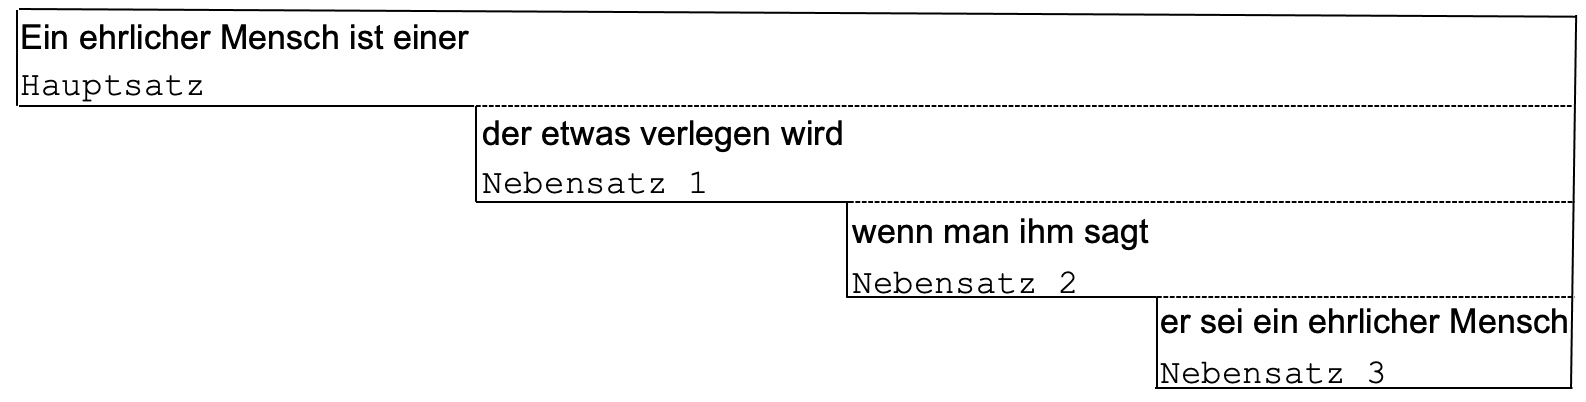
\includegraphics[width=12cm]{figures/Satzbild_Frisch.jpeg}
    %% Abbildung 



\noindent\resizebox{\textwidth}{!}{
	
	\begin{tabular}{ lll }
	
		\hline
		\multicolumn{1}{ | l}{} &&\multicolumn{1}{ l | }{\makecell[l]{stört den Wanderer \\ \small{\textcolor{gray}{Hauptsatz}}}}  \\ \cline{3-3} \sbdashline{1-2}
		
		\multicolumn{1}{ | l }{\makecell[l]{Dass die Leute den Wald verschmutzen \\ \small{\textcolor{gray}{Nebensatz 1}}}} & \multicolumn{1}{ l | }{} & \\ \cline{1-1} \sbdashline{2-2}
		
		& \multicolumn{1}{ | l | }{\makecell[l]{indem sie ihren Müll abladen \\ \small{\textcolor{gray}{Nebensatz 2}}}} & \\ \cline{2-2} 
		
	
	\end{tabular}
}





    \caption{Satzbild zu Satz (\ref{ex:NeSa_Gefüge})}
    \label{Abb:Satzbild}
\end{figure}
 
Der gesamte Satz ist ein Hauptsatz. Hierfür steht die obere durchgezogene Linie. Auf der Hauptsatzebene steht das Hauptsatzgerüst \textit{stört den Wanderer}. Dieser Teilsatz ist unterstrichen. Der Hauptsatz geht jedoch weiter, wofür die gestrichelte Linie steht. Die Nebensätze sind direkt und indirekt eingebettete Bestandteile des Hauptsatzes. Eine Hierarchieebene unter dem Hauptsatzgerüst steht das Nebensatzgerüst von Nebensatz 1 \textit{dass die Leute den Wald verschmutzen}. Der Nebensatz 2 \textit{indem sie ihren Müll abladen} ist ein eingebetteter Bestandteil von Nebensatz 1. Deshalb steht er wieder eine Ebene tiefer. Die gestrichelten Linien symbolisieren die jeweilige Einbettung in die höhere Ebene. Der Nebensatz 2 ist nicht direkt in den Hauptsatz eingebettet, sondern indirekt über Nebensatz 1.    

Bevor es um einzelne Satzglieder geht, ist ihre Abgrenzung von Attributen, die Teile von Satzgliedern sind, wesentlich. Denn \gqq{[d]ie Satzgliedanalyse}, so \citet[80]{Welke2007}, \gqq{steht und fällt mit der Unterscheidung} zwischen Satzgliedern und Attributen. Um diese geht es in dem folgenden Abschnitt~\ref{section:SatzgliederundAttribute}. Zuvor wollen wir jedoch, wie angekündigt, in dem folgenden Exkurs auf den Satzbegriff zurückkommen.

\begin{Exkurs}{Sätze und Nichtsätze?}\label{Exkurs:Satz_Nichtsatz}

Der Satzbegriff, mit dem wir im Rahmen der Satzgliedanalyse arbeiten, ist mindestens an das Vorhandensein eines Verbs als Prädikat gebunden. Er ist also formbezogen. Die von ihm abhängigen Ergänzungen erhalten ihre Form und Funktion erst in ihrer jeweiligen Beziehung zum Prädikat. Ohne Prädikat gibt es keine Satzgliedfunktionen wie Subjekt (vom Prädikat) oder Objekt (vom Prädikat). 

In der Einführung ins Kapitel~\ref{chapter:Feldermodell} haben wir die zentralen sprachlichen Handlungen aufgeführt, die wir mithilfe von Verberst- und Verbzweitsätzen vollziehen (vgl. \textit{Illokution} in Definition~\ref{Def_Illokution}). Auch bestimmte Verbletztsätze verfügen über illokutives Potenzial, dessen wir uns beim selbständigen Gebrauch bedienen: \textit{Dass du mir pünktlich kommst!} Nun gibt es aber auch Äußerungen, die wir wie Sätze gebrauchen, ohne dass sie ein Prädikat enthalten. So verstehen wir (\ref{ea:Landleben}) als Behauptung, (\ref{ex:jetzt_ins_Freiland?}) als Frage und (\ref{ex:jetzt_ins_Moma!}) als Aufforderung. Ebenso denke man an Ausrufe wie \textit{um Himmels willen} in (\ref{ex:himmels_Willen}) und sogenannte Satzäquivalente wie \textit{doch} in (\ref{ex:doch}).

\ea \label{ea:KME}
\ea \label{ea:Landleben} Landleben auf der Potsdamer Straße – mit Ziegen aus dem Öko-Dorf.\footnote{Berliner Zeitung, 19.09.2005.}
\ex \label{ex:jetzt_ins_Freiland?} Jetzt ins Freiland? Mit mir nicht.\footnote{Berliner Zeitung, 06.03.1998.}
\ex \label{ex:jetzt_ins_Moma!} Jetzt ins MoMa! Die Wartezeit beträgt weniger als 45 Minuten.\footnote{Berliner Zeitung, 08.07.2004.}
\ex \label{ex:himmels_Willen} Sie sind ein Fan? Um Himmels willen. Ich gehöre nicht zur Zielgruppe dieser Sendung.\footnote{Berliner Zeitung, 03.03.2003.}
\ex\label{ex:doch} Oder hat sich in der Zwischenzeit nichts geändert? Doch.\footnote{Berliner Zeitung, 29.04.2005.}
\z 
\z  

Vor unserem formbezogenen Hintergrund handelt es sich bei den Äußerungen in (\ref{ea:KME}) nicht um Sätze, sondern um \textit{kommunikative Minimaleinheiten}, wie \citet[86]{ZifHoffStr1997} solche Äußerungen bezeichnen: \gqq{Mit kommunikativen Minimaleinheiten können sprachliche Handlungen vollzogen werden. Der Satz hingegen ist im Rahmen dieser Grammatik eine formbezogen bestimmte Einheit. Sätze enthalten ein finites Verb [\ldots]}. 

\citet[320--321]{Hentschel_Weydt2021} machen darauf aufmerksam, dass auch Äußerungen ohne finites Verb bestimmten Stellungsregeln folgen müssen und dass solche im Rahmen des formbezogenen Ansatzes \textit{nicht-Sätze} in vielen Kontexten viel angemessener sind als die entsprechenden Äußerungen mit einem finiten Verb. Deshalb definieren sie den Satz nach dem Kriterium der syntaktischen Selbständigkeit. Hier lässt sich mit \citet[119]{Engel2009} kritisch nach der Bedeutung von Selbständigkeit fragen: Wie selbständig ist ein Satz, der nur in sehr bestimmten, pragmatisch definierten Situationen zulässig und verständlich ist? Aufgrund der Stellungsregularitäten, die \citet[44]{Musan2021_SGA} auf ein mitverstandenes, aber ausgelassenes Prädikat zurückführt (vgl. \textit{Koordinationsellipse} im Abschnitt~\ref{subsection:SatzgefügeSatzreihe}), bezeichnet sie auch prädikatslose Äußerungen wie in (\ref{ea:KME}) als Sätze. Aufgrund der hier angerissenen Definitionsprobleme gibt \citet[77]{Rothstein2023Syntax} die wohl weiteste Definition von Satz als \gqq{grammatisch vollständige Verbindung mehrerer Konstituenten (wobei sogenannte Einwortsätze, z. B. Ja!, aus nur einer Konstituente bestehen können).}  

Für \citet[70--71]{Welke2005Temp} liegt das Problem in der Definitionsmethode. Anstatt nach \textit{einem} Merkmal zu suchen, das alle Mitglieder einer Kategorie auszeichnet und von anderen Kategorien abgrenzt, plädiert er für eine prototypische Definition: Nicht allen Kategoriemitgliedern kommt dasselbe Merkmal als Invariante zu. Sie weisen verschiedene, über den Prototyp miteinander verbundene Merkmale auf. Ein prototypischer Satz verfügt demnach mindestens über ein finites Verb als Prädikat und über ein illokutives Potenzial. Weniger typische Sätze verfügen nur über eines der beiden, vom Prototyp abgeleiteten Merkmale. Viele Nebensätze verfügen nicht über ein illokutives Potential, aber über ein Prädikat. Auch Infinitive und Partizipien können als Prädikat fungieren, wenn auch nur mit eingeschränktem illokutivem Potenzial. Prädikatslose Äußerungen können als weniger typische Sätze über ein illokutives Potenzial verfügen.

Wesentlich ist die Einsicht, dass auch prädikatslose Äußerungen strukturiert und funktional sind. Hierauf weist besonders \citet[170]{Agel2017} hin, der den prädikatshaltigen Sätzen als Szenario-Ausdruck prädikatslose Nichtsätze als Impressio-Ausdruck komplementär gegenüberstellt: Es handelt sich um \gqq{zwei Grundtypen (einzelsprachlichen) darstellungsfunktionalen Agierens}. Bei Szenario-Ausdrücken bekommen die verbalen Ergänzungen -- anders als die autonom kodierenden Angaben (vgl. Abschnitt~\ref{subsubsection:TestINSP}) -- ihre Werte vom Prädikat zugewiesen. Bei Impressio-Ausdrücken müssen wir den nicht autonom kodierenden Formen, so \citet[170]{Agel2017}, \gqq{auf der Grundlage von satzhaften Analogieerfahrungen und Inferenzen auf der Basis der internen Formen und deren semantischen Beziehungen zueinander} semantische Werte zuweisen, ohne dass diese von einem Prädikat aus berechenbar wären.\footnote{Im Rahmen der grammatischen Textanalyse schlägt \citet[175--191]{Agel2017} eine sehr feine Binnendifferenzierung unter den Nichtsätzen vor, auf die wir nicht weiter eingehen.} Sehen wir uns diesbezüglich in (\ref{ea:Tadellöser}) prädikatslose Äußerungen auf den ersten Seiten des Romans \textit{Tadellöser und Wolff} von Walter Kempowski an. Der Protagonist erzählt den Umzug in eine neue Wohnung.

\ea \label{ea:Tadellöser}
\ea \label{ea:Tadellöser1} Morgens hatten wir noch in der alten Wohnung auf grauen Packerkisten gehockt und Kaffee getrunken (gehört das uns, was da drin ist?). Helle Felder auf den nachgedunkelten Tapeten.\footnote{Walter Kempowski: \textit{Tadellöser und Wolff}. München: Penguin 2016 [1979], S. 1.}
\ex \label{ex:Tadellöser2} Ich teilte mit meinem Bruder Robert das Zimmer. Sechs
Jahre älter als ich. Das blonde Haar stark gewellt, wie die Wogen des Sees Genezareth, in der Bilderbibel, auf denen Jesus wandelt.\footnote{Walter Kempowski: \textit{Tadellöser und Wolff}. München: Penguin 2016 [1979], S. 11.}
\ex \label{ex:Tadellöser3} Mein Vater kaufte sich ein neues Rad. Das alte, mit Dorn
zum Hintenaufsteigen, war verrostet. Dazu einen Kleppermantel, dessen Schöße hochknöpfbar waren.\footnote{Walter Kempowski: \textit{Tadellöser und Wolff}. München: Penguin 2016 [1979], S. 14.}
\z 
\z 

In (\ref{ea:Tadellöser1}) müssen wir eine formal nicht angewiesene Beziehung zwischen der Wortgruppe \textit{Helle Felder auf den nachgedunkelten Tapeten} und dem Vortext herstellen. Da wir diese Wortgruppe nicht direkt in den Vortext einbauen können, interpretieren wir sie als Objekt in einem bekannten und hier plausiblen Existenzausdruck: \textit{Es gab helle Felder auf den nachgedunkelten Tapeten}. Möglich und nicht weniger plausibel wäre auch die Interpretation als Subjekt einer Verortungskonstruktion, die durch die autonom kodierende Wortgruppe \textit{auf den nachgedunkelten Tapeten} motiviert ist: \textit{Helle Flecken befanden sich auf den nachgedunkelten Tapeten}.

In (\ref{ex:Tadellöser2}) interpretieren wir die Wortgruppe \textit{Sechs Jahre älter als ich} als eine Eigenschaft, die dem Bruder Robert zugeschrieben wird. Hierfür nutzen wir das eingeübte prädikative Muster mit dem Verb \textit{sein} und ergänzen den Bruder als Subjekt: \textit{Mein Bruder Robert war/ist sechs Jahre älter als ich}. Auch der nächsten Wortgruppe \textit{das blonde Haar stark gewellt, wie die Wogen des Sees Genezareth, in der Bilderbibel, auf denen Jesus wandelt} müssen wir zur Interpretation einen Wert zuweisen, den sie in Ermangelung eines Hauptprädikats formal nicht zugewiesen bekommt. Wir verstehen sie als Objekt zum Prädikat \textit{haben} oder \textit{tragen} und ergänzen wieder das dazugehörige Subjekt: \textit{Mein Bruder Robert hatte das blonde Haar stark gewellt \ldots} oder \textit{Mein Bruder Robert trug das blonde Haar stark gewellt \ldots}. Ebenso möglich wäre es, die formal nicht angewiesene Stellung der Wortgruppe analog zu dem vorherigen Fall im Rahmen einer Eigenschaftszuweisung zu verstehen: \textit{Sein blondes Haar war stark gewellt \ldots}. 

In (\ref{ex:Tadellöser3}) haben wir es bei \textit{Dazu einen Kleppermantel, dessen Schöße hochknöpfbar waren} mit einer NP im Akkusativ zu tun. Da es kein Prädikat gibt, können wir der Wortgruppe nicht den erwartbaren Wert Akkusativobjekt zuweisen. Wir orientieren uns am Vortext und interpretieren diese Wortgruppe als Akkusativobjekt zum Prädikat \textit{kaufte} im ersten Satz.   

In den Textpassagen in (\ref{ea:Tadellöser}) sind wir auf Formen gestoßen, deren syntaktische und semantische Funktion formal nicht durch ein übergeordnetes Prädikat bestimmt ist. Wir haben sie in Analogie zu uns bekannten Sätzen und im Rahmen der vorangehenden Sätze assoziativ interpretiert. Eben hierin liegt auch der Reiz solcher prädikatslosen Äußerungen gegenüber Szenario-Ausdrücken mit Prädikat. Der Leser bzw. die Leserin muss ohne formale Anweisung die Formen in mögliche (früher schon erfahrene) prädikative Strukturen und in den laufenden Text im Sinne syntaktisch-semantischer Werte einbetten. Beim Lesen entsteht aus formalen Reihungen, aus Erinnerungsfetzen und Eindrücken (Impressionen) etwas Zusammenhängendes.

\end{Exkurs}



\section{Attribute als Teile von Satzgliedern}\label{section:SatzgliederundAttribute}


Attribute\is{Attribut} hängen von nicht-verbalen Bezugswörtern als Köpfen ab und stehen somit nur in mittelbarer Beziehung zum Prädikat.\footnote{Diese weite Bestimmung des Attributbegriffs folgt \citet[110]{Elst_Habermann_SynAn}, \citet[502]{HelbigBuscha}, \citet[81]{Welke2007}, \citet[152]{OehlSeiler2013} und \citet[698]{Agel2017}. \citet[259]{Eisenberg2020_Satz} geht von einem engen Attributbegriff als Prototyp aus, erweitert ihn aber. \citet[351]{Schaefer2018_3Aufl} schränkt, wie das traditionell üblich war, den Attributbegriff auf Konstituenten der Nominalphrase ein. Einen Überblick zur Begriffsgeschichte geben \citet[307--309]{FuhrhopThierrof2005}, speziell zur jüngeren Abgrenzungsproblematik \citet[231--233]{Engel2011Attribut}.} Den Prototyp des Attributs bilden die im Abschnitt~\ref{section:NP} aufgezeigten Möglichkeiten, einen nominalen Kopf insbesondere\is{Attribut!Typen} durch Adjektivphrasen, NPs im Genitiv, durch PPs und Relativsätze auszubauen. Deshalb spricht man von Adjektivattributen (\ref{ea:Adjektivattribut}), Genitivattributen (\ref{ex:Genitivattribut}), Präpositionalattributen (\ref{ex:PPAttribut}) und Relativsatzattributen (\ref{ex:Relativsatzattribut}). 

\ea \label{ea:NAttribute}
\ea \label{ea:Adjektivattribut} Die \textit{große} Frau tanzt.
\ex \label{ex:Genitivattribut} Die Frau \textit{meines Bruders} tanzt.
\ex \label{ex:PPAttribut} Die Frau \textit{mit dem Hut} tanzt.
\ex \label{ex:Relativsatzattribut} Die Frau, \textit{die einen Hut trägt}, tanzt.
\z 
\z 

Durch Attribute wird diejenige Entität, die von einer NP bezeichnet wird, ihr Referent, genauer charakterisiert, oder die Menge der möglichen Referenten wird eingeschränkt. So wird in (\ref{ea:Adjektivattribut}) entweder die Person, die wir mit \textit{die Frau} bezeichnen, näher beschrieben oder aber, wenn mehrere Frauen in Frage kommen, klargestellt, um welche Frau es geht, hier um die große und nicht um die kleine.  

Attribute können nicht alleine im Vorfeld (vgl. Abschnitt~\ref{subsection:Vorfeld}) stehen. Sie können nur zusammen mit ihrem Kopf und der von diesem gebildeten Phrase im Vorfeld stehen, wenn diese Phrase ein Satzglied ist. Alleine sind sie nicht vorfeldfähig (\ref{ea:NAttributeTests}), zumindest nicht bei gleicher Bedeutung. Hierfür steht die Raute bei (\ref{ex:PPAttribut_pron}) im Vergleich zu (\ref{ex:PPAttribut}). 

\ea \label{ea:NAttributeTests}
\ea  [*] {\textit{Große} tanzt die Frau.}\label{ea:Adjektivattribut_top}
\ex [*] {\textit{Meines Bruders} tanzt die Frau.}\label{ex:Genitivattribut_erfragbar}
\ex [\#] {\textit{Mit dem Hut} tanzt die Frau.}\label{ex:PPAttribut_pron}
\ex [*] {\textit{Die einen Hut trägt,} tanzt die Frau.}\label{ex:Relsatz_VF}
\z 
\z 

In Bezug auf die Beispiele in (\ref{ea:NAttribute}) mag die Frage aufkommen, warum wir die Artikel nicht zu den Attributen zählen. Auch sie hängen vom Substantiv und nicht vom Verb ab.\footnote{\citet[235]{Engel2011Attribut} zählt aufgrund der Abhängigkeit vom Substantiv auch Artikel zu den Attributen. Die \citet[441, §722]{Duden2022} zählt nur die Possessivartikel wie \textit{sein} zu den Attributen, da diese Artikel und gleichzeitig possessive Attribute seien: \textit{das Haus von Paul}, \textit{Pauls Haus} und  \textit{sein Haus}. Für \citet[321--322]{FuhrhopThierrof2005} ist das wesentliche Argument gegen den Attributstatus von Artikeln, dass diese ausschließlich als Funktionsträger in Nominalphrasen vorkommen und dabei selbst nicht durch Attribute erweiterbar sind.} Wir zählen Artikel grundsätzlich nicht zu den Attributen. Artikel sind obligatorische funktionale Bestandteile von Nominalphrasen (vgl. Abschnitt~\ref{section:NP}). Sie zeigen deren grammatische Merkmale an und setzen die Bedeutung des Substantivs zu konkreten Individuen bzw. Entitäten in Beziehung (Determination). Attribute sind fakultativ und reichern die Bedeutung des Substantivs bzw. der Nominalphrase an (Modifikation). Funktional kann es durchaus zu Überschneidungen zwischen Artikeln und Attributen kommen.

Wir haben gesagt, dass Attribute nur zusammen mit ihrem Bezugswort im Vorfeld stehen können. Deshalb ist (\ref{ex:Relsatz_VF}) ungrammatisch. Allerdings erscheinen Relativsatzattribute häufig von ihrem im Mittelfeld (vgl. Abschnitt~\ref{subsection:Mittelfeld}) stehenden Bezugswort getrennt, indem sie wie in (\ref{ea:RelSatzNF}) im Nachfeld (vgl. Abschnitt~\ref{subsection:Nachfeld}) stehen.

\ea \label{ea:RelSatzNF} Er hat die Frau gegrüßt, die einen Hut trägt.
\z 


Auch bestimmte andere Attribute können getrennt von ihrem Bezugswort stehen. Entweder steht das Bezugswort wie in (\ref{ea:Wer_von_Split}) allein im Vorfeld und das Attribut steht im Mittelfeld oder das Attribut steht wie in (\ref{ex:PP_Attribut_Split}) allein im Vorfeld und das Bezugswort steht im Mittelfeld.\footnote{Bei den Stellungen zwischen Kopf und \textit{von}-Attribut in (\ref{ea:Attribut_Split}) handelt es sich um eine Element-Menge-Trennung. Andere sogenannte Splitkonstruktionen bildet man mit \textit{was für}, \textit{w- alles}, \textit{w- an} und \textit{w-} mit substantiviertem Adjektiv: \textit{Was hat er für ein Problem?}; \textit{Wer hat alles zugestimmt?}; \textit{Was gibt es noch an Problemen?}; \textit{Was gibt es Neues?} Cf. \citet[145--146]{Pafel1995}.}

\largerpage
\ea \label{ea:Attribut_Split}
\ea \label{ea:Wer_von_Split} Wer hat \textit{von den Abgeordneten} gegen den Antrag gestimmt?
\ex \label{ex:PP_Attribut_Split} \textit{Von den Abgeordneten} hat eine Mehrheit gegen den Antrag gestimmt.
\z 
\z   

Dennoch handelt es sich bei \textit{von den Abgeordneten} in (\ref{ea:Wer_von_Split}) um ein Attribut von \textit{wer} und in (\ref{ex:PP_Attribut_Split}) um ein Attribut von \textit{Mehrheit}. Das Attribut schränkt die Menge der unter \textit{wer} bzw. \textit{eine Mehrheit} fallenden Personen ein. Das Attribut steht nicht in direkter Beziehung zum Prädikat: *\textit{Von den Abgeordneten hat gegen den Antrag gestimmt}. In beiden Fällen können das Bezugswort und das Attribut zusammen das Vorfeld besetzen (\ref{ea:Attribut_kein_Split}).

\ea \label{ea:Attribut_kein_Split}
\ea \label{ea:Wer_von_PP} Wer \textit{von den Abgeordneten} hat gegen den Antrag gestimmt?
\ex \label{ex:Mehrheit_von_PP} Eine Mehrheit \textit{von den Abgeordneten} hat gegen den Antrag gestimmt.
\z 
\z   


\begin{Definition}{Attribut}
    
\noindent Attribute sind Wörter oder Wortgruppen eines Satzes, die keine direkte Beziehung zum Prädikat haben und die folglich keine Satzglieder sind. Attribute sind fakultative Bestandteile von Satzgliedern. Der Prototyp hängt vom Kopf einer NP ab und beschreibt deren Referenten näher oder grenzt den Referenzbereich ein.    
\end{Definition}




Als besondere\is{Attribut} Attribute betrachten wir die im Exkurs~\ref{subsection:Apposition} diskutierten lockeren (\ref{ea:Attr_lockere_Apposition}) und engen Appositionen (\ref{ex:Attr_engeApposition}). Hierzu gehören auch die Stoff- bzw. Inhaltsangaben als Attribut zu Mengen- und Maßbezeichnungen (\ref{ex:Maß_Inhalt}). 

\ea \label{ea:NAttribut_Apposition}
\ea \label{ea:Attr_lockere_Apposition} Berlin, \textit{die Bundeshauptstadt}, ist Deutschlands größte Stadt.
\ex \label{ex:Attr_engeApposition} Die Bundeshauptstadt \textit{Berlin} ist Deutschlands größte Stadt.
\ex \label{ex:Maß_Inhalt} Zwei Flaschen \textit{Saft} sind noch da.
\z 
\z 

Da wir einen weiten\is{Attribut} Attributbegriff ansetzen, sprechen wir auch beim Ausbau von APs (\ref{ea:A_Attribut}) und PPs (\ref{ex:P_Attribut}) von Attributen. 

\ea \label{ea:XAttribute}
\ea \label{ea:A_Attribut} Die \textit{auf ihren Enkel} stolze Oma lacht.
\ex \label{ex:P_Attribut} Sie traf ihn \textit{kurz} vor Mitternacht.
\z 
\z 

Die PP \textit{auf ihren Enkel} in (\ref{ea:A_Attribut}) ist eine Ergänzung des Adjektivs \textit{stolze}. Auf der Ebene des Satzes handelt es sich bei \textit{auf ihren Enkel} um ein Attribut von \textit{stolze}. Beide zusammen sind als AP Attribut zu \textit{Oma}.\footnote{\citet[68]{Musan2021_SGA} bezeichnet auch die Ergänzungen von Adjektiven als Objekte. Die PP \textit{auf ihren Enkel} in (\ref{ea:A_Attribut}) wäre demzufolge ein Präpositionalobjekt zu \textit{stolze}. Wir reservieren den Objektbegriff für die Ebene der Satzglieder. Will man differenzieren zwischen valenziell verankerten Attributen und frei hinzufügbaren, so kann man wie \citet[493]{HelbigBuscha} von valenzbedingten und valenzunabhängigen Attributen sprechen.} Die ganze NP \textit{die auf ihren Enkel stolze Oma} ist Subjekt von \textit{lacht}. In (\ref{ex:P_Attribut}) ist \textit{kurz} ein Adjektivattribut der PP \textit{vor Mitternacht}. Beide zusammen bilden als komplexe PP \textit{kurz vor Mitternacht} ein Satzglied, das als temporales Adverbial fungiert.  

Am Beispiel\is{Attribut!komplex} der NP (vgl. Abschnitt~\ref{section:NP}) und der AP (vgl. Abschnitt~\ref{section:AP}) haben wir Folgendes gesehen: Mehr als ein Attribut kann sich auf einen Kopf beziehen. Das hat Auswirkungen auf die Kommasetzung (\textit{kluge, unterhaltsame Bücher} versus \textit{spannende französische Bücher}). Adjektivattribute können also sehr komplex sein, da sie intern wiederum Phrasen bilden. Eine besondere Komplexität von Attributen kann dadurch entstehen, wenn wir VPs wie \textit{ein Haus bauen} nominalisieren\is{Substantivierung}, also in eine NP wie \textit{der Bau eines Hauses} umwandeln.

In Kapitel \ref{chap:Konstituenz} haben wir gezeigt, dass der Ausbau des Verbkopfes zum Satz analog beschreibbar ist wie der Ausbau nominaler Köpfe zur NP. Mit dem\is{Attribut} Attributbegriff trennen wir beide Ausbau-Ebenen.\footnote{Viele Grammatikmodelle basieren auf der grundlegenden Unterscheidung zwischen Köpfen auf der einen Seite und Ergänzungen (Argumenten) sowie Angaben (Adjunkten) auf der anderen Seite. Ein Äquivalent zum Attributbegriff gibt es nicht.} Für den Attributbegriff und damit die Trennung der verbalen von allen anderen Ebenen sprechen formale und funktionale Gründe. \citet[46]{Eichinger1995} schreibt, dass es sich bei verbaler und nominaler Ebene um \gqq{funktionale Kategorisierungsstufen eigener Art} handele. \citet[254]{Welke2011} hält die substantivische und verbale Konstruktion für \gqq{grundverschieden}.

In\is{Satzglied!versus Attribut} der verbalen Konstruktion, also auf Ebene der Satzglieder, spielen NPs im Nominativ, im Akkusativ und im Dativ eine primäre Rolle für die Kodierung von Subjekt, Akkusativobjekt und Dativobjekt.\footnote{Im Bereich der verbalen Ergänzungen haben wir den Genitiv in Abschnitt~\ref{subsubsection:TestFOSP} als Relikt beschrieben.} Diese sättigen die Valenzanforderungen des Prädikats. Das Prädikat weist den vom Subjekt und von den Objekten Bezeichneten Rollen zu, was in Abschnitt~\ref{subsubsection:TestINSP} als\is{Prädikation} Prädikation beschrieben wurde. Auf dieser Grundlage bilden wir Sätze. Mit Sätzen handeln wir, indem wir \zB etwas aussagen, befehlen oder fragen. 

In der nominalen Konstruktion, also auf\is{Attribut!komplex} Attributebene, spielen Adjektivattribute und NPs im Genitiv die zentrale Rolle. Diese sättigen typischerweise keine valenziellen Forderungen. Daher zeichnet sich die nominale Attribution (im Vergleich zum Verbalbereich) durch große Variation aus.\footnote{Cf. \citet[318]{FuhrhopThierrof2005}.} Originäre (nicht vom Verb oder Adjektiv abgeleitete) Nomen prädizieren typischerweise nicht über den Attributen. Mit NPs allein treffen wir keine expliziten Aussagen, erteilen keine expliziten Befehle und stellen keine expliziten Fragen. Hierzu muss die NP Teil einer finiten VP werden. Durch Attribute erweiterte NPs sind als dichte Informationsverpackungen ein Merkmal der Bildungssprache.\footnote{Seit dem 16. Jahrhundert wird die NP durch Attribution immer komplexer. Das führt letztlich zur Entwicklung des für die Bildungssprache typischen Nominalstils. Cf. \citet[36--38]{Admoni1973}, \citet[6]{CziczaHenningetal2012}.} Ihre korrekte Bildung und ihr Verständnis setzen voraus, den Kopf als Bezugswort zu erkennen und die Bedeutungen der Attribute schrittweise auf das vom Bezugswort Bezeichnete zu übertragen. Wir illustrieren dies anhand der eingeklammerten komplexen NP in (\ref{ea:komplexeNPAttribut}), die wir in (\ref{ex:expl1}), (\ref{ex:expl2}) und (\ref{ex:expl3}) in explizite Prädikationen überführen. Das Präpositionalattribut \textit{in einer demokratischen Gesellschaft} kann auch wie in (\ref{ex:expl4}) als Attribut auf den nominalen Kern \textit{Grundlage} bezogen werden.  

\ea \label{ea:Attributbeispiel}
\ea \label{ea:komplexeNPAttribut} Sie (die Medienbildung, M.F.) ist [...] eine essentielle Voraussetzung für Ausbildungs- und Studierfähigkeit und [Grundlage lebenslangen Lernens in einer demokratischen Gesellschaft].\footnote{Senatsverwaltung für Bildung, Jugend und Familie: Rahmenlehrplan 1--10 kompakt. Themen und Inhalte des Berliner Unterrichts im Überblick. 2017. \url{https://www.berlin.de/sen/bildung/unterricht/faecher-rahmenlehrplaene/rahmenlehrplaene/} (08.05.19).}
\ex \label{ex:expl1} Die Grundlage betrifft das Lernen.
\ex \label{ex:expl2} Das Lernen geschieht lebenslang.
\ex \label{ex:expl3} Das lebenslange Lernen findet in einer demokratischen Gesellschaft statt.
\ex \label{ex:expl4} Die Grundlage betrifft das lebenslange Lernen und liegt in einer demokratischen Gesellschaft.
\z 
\z 

Aber es gibt auch Gemeinsamkeiten zwischen der Ebene der\is{Satzglied!versus Attribut} Satzglieder und der\is{Attribut!versus Satzglied} Attribute. Eine Gemeinsamkeit betrifft die Abhängigkeitsrelation. Die Satzglieder hängen vom Prädikat ab und die Attribute von einem nominalen Kopf. Wenn wir im Bild der Matroschka bleiben, dann sind die Attribute kleinere Matroschkas, die in den größeren Satzglied-Matroschkas stecken. Formal können sowohl Satzglieder als auch Attribute durch PPs realisiert werden, wie einführend anhand der doppeldeutigen Überschrift \textit{Polizei jagt Verbrecher mit Oldtimer} illustriert wurde. Analog dazu können wir die kursiv gedruckte PP \textit{durch die Polizei} in (\ref{ea:durchPolizei}) als Satzglied\is{Satzglied!versus Attribut} oder als Attribut\is{Attribut!versus Satzglied} interpretieren.

\ea \label{ea:durchPolizei} Dieser Bereich wird zur Verhütung von Straftaten \textit{durch die Polizei} videoüberwacht.\footnote{\url{https://de.wikipedia.org/wiki/Mehrdeutigkeit} (02.04.18).} 
\z

Dem\is{Ambiguität!syntaktisch} primären Verständnis zufolge ist die PP als Satzglied direkt dem Prädikat untergeordnet: \textit{durch die Polizei videoüberwacht werden}. Sie besteht die in Kapitel \ref{chap:Konstituenz} vorgestellten Satzgliedtests. Sie ist durch ein Pronomen erfragbar (\ref{ea:durchdiePolizeiErfragbar}) und voranstellbar (\ref{ex:durchdiePolizeiVoranstellbar}). 

\ea \label{ea:SGTestdurchdiePolizei}
\ea \label{ea:durchdiePolizeiErfragbar} \textit{Durch wen} wird dieser Bereich zur Verhütung von Straftaten videoüberwacht?
\ex \label{ex:durchdiePolizeiVoranstellbar} \textit{Durch die Polizei} wird dieser Bereich zur Verhütung von Straftaten videoüberwacht. 
\z 
\z 

Möglich (wenn auch unwahrscheinlich) ist jedoch auch die Einbettung der PP unter \textit{Straftaten}, ihr Gebrauch also als Attribut in \textit{Straftaten durch die Polizei} mit der Bedeutung \gq{Straftaten, die durch die Polizei verübt werden}. In diesem Fall besteht die PP \textit{durch die Polizei} nicht die Satzgliedtests. Sie ist nicht alleine erfragbar und voranstellbar nur innerhalb des Satzglieds, dessen Teil sie ist  (\ref{ea:durchdiePolizeiAttribut}).

\ea \label{ea:durchdiePolizeiAttribut} \textit{Zur Verhütung von Straftaten durch die Polizei} wird dieser Bereich videoüberwacht.
\z 

Trotz unterschiedlicher Einbettung, einmal als\is{Satzglied!versus Attribut} Satzglied und einmal als\is{Attribut!versus Satzglied} Attribut, drückt die PP auf ähnliche Weise die verursachende Entität aus. 

Auch Adverbien können neben ihrem primären Gebrauch als Satzglied (\ref{ea:AdvSG}) postnominal als Attribut wie in (\ref{ex:AdvAttribut}) gebraucht werden. 

\ea \label{ea:AdvAttributSatzglied}
\ea \label{ea:AdvSG} Der Film lief \textit{gestern}.
\ex \label{ex:AdvAttribut} Der Film \textit{gestern} hat viele begeistert.
\z 
\z 

Ein\is{Satzglied!zum Attribut} und\is{Attribut!aus Satzglied} derselben Form wie der PP in (\ref{ea:durchPolizei}) oder der Adverbphrase in (\ref{ea:AdvAttributSatzglied}) kommt je nach Bezugsgröße eine andere syntaktische Funktion zu. Die Funktion eines sprachlichen Ausdrucks ist nur in Beziehung zu einem anderen Ausdruck zu bestimmen.    

\citet[35, 55]{Agel2017} bezeichnet die Identität auf verschiedenen Funktionsebenen als \gqq{Recycling} und schreibt: \gqq{Analoge semantische Werte [...] werden vertikal -- hierarchisch -- durch die funktionalen Ebenen grammatisch \gq{durchgereicht}}. Hierbei handelt es sich, so \citet[751]{Agel2017}, um \gqq{ein elementares \textit{funktionales} Merkmal des grammatischen Systems}. Neues wird weitgehend analog zu Bestehendem (und daher ökonomisch) nachgebildet.\footnote{Cf. \citet[295]{Langacker1991}.} Lokale und temporale Attribute wie \textit{dort} und \textit{gestern} in \textit{der Baum dort} und \textit{der Film gestern} sind durch Analogie zur Adverbialebene motiviert, wie in \textit{der Baum steht dort} und \textit{der Film lief gestern}. Andere Attribute wie \textit{auf gutes Wetter} in \textit{die Hoffnung auf gutes Wetter} sind durch Analogie zur Objektebene motiviert, wie in \textit{sie hoffen auf gutes Wetter}.

Dieses \textit{Recycling} zeigt sich besonders bei der Ableitung von\is{Nominalisierung} Nomen aus Verben (deverbale Nomen). Da der Nominalstil typisch für die Schul- und Bildungssprache\footnote{Cf. \citet[489--490]{GogolinDuarte2016}.} ist, gehen wir etwas genauer darauf ein. Wenn das Verb eine Präposition regiert wie \textit{auf etwas hoffen} (\ref{ea:hoffenauf}), so erbt das abgeleitete Nomen \textit{Hoffnung} diese Präposition (\ref{ex:Hoffnungauf}). Die Nominativ-NP in Subjektfunktion kann bei Nominalisierung als Genitiv-NP, bei Eigennamen wie \textit{Paul} in (\ref{ea:hoffenauf}) postnominal, ausgedrückt werden.

\ea \label{ea:Nominalisierung}
\ea \label{ea:hoffenauf} Paul hofft \textit{auf gutes Wetter}.
\ex \label{ex:Hoffnungauf} Pauls Hoffnung \textit{auf gutes Wetter}
\z 
\z 

Aus dem Präpositionalobjekt in (\ref{ea:hoffenauf}) ist in (\ref{ex:Hoffnungauf}) ein Präpositionalattribut\is{Attribut!versus Satzglied} geworden und aus dem Nominativsubjekt ein Genitivattribut.  Während in (\ref{ea:hoffenauf}) explizit eine Aussage gemacht wird, ist dies in (\ref{ex:Hoffnungauf}) nicht, oder nur implizit der Fall. Aus dem Verb ist ein Nomen geworden. Die aus dem Nomen gebildete NP kann als Satzglied einem anderen Prädikat (\ref{ea:NPalsneuesObjekt}) oder als Attribut einem Nomen (\ref{ex:NPalsAttribut}) untergeordnet werden. So können wir viele Informationen kompakt auf der Nominalebene unterbringen. 

\ea \label{ea:Nominalisierungsdichte}
\ea \label{ea:NPalsneuesObjekt} Anna spottet über \textit{Pauls Hoffnung auf gutes Wetter}.
\ex \label{ex:NPalsAttribut} \textit{Annas Spott über Pauls Hoffnung auf gutes Wetter} ist allen bekannt.
\z 
\z 

Analog zur Umfunktionierung der PP in (\ref{ea:Nominalisierungsdichte}) können auch Nebensätze von Satzgliedern (\ref{ea:NeSaObj}) zu\is{Attribut!Nebensatz} Attributen (\ref{ea:NeSaAttr}) umfunktioniert werden. 

\ea \label{ea:NeSaAttrSG}
\ea \label{ea:NeSaObj} Paul hofft, \textit{dass gutes Wetter wird}.
\ex \label{ea:NeSaAttr} Pauls Hoffnung, \textit{dass gutes Wetter wird}
\z 
\z 

Das\is{Satzglied!Recycling} Gleiche gilt für Infinitivgruppen: In (\ref{ea:InfObj}) ist \textit{Anna wiederzusehen} ein Satzglied, in (\ref{ex:InfAttr}) hingegen ein Attribut.

\ea \label{ea:InfAttrSG}
\ea \label{ea:InfObj} Paul hofft, \textit{Anna wiederzusehen}.
\ex \label{ex:InfAttr} Pauls Hoffnung \textit{Anna wiederzusehen}
\z 
\z 


Wenn\is{Nominalisierung} Verben über ein Akkusativobjekt verfügen wie \textit{etwas beantworten}, dann wird dieses bevorzugt als Genitivattribut an das deverbale Nomen vererbt. Das ist insbesondere bei Handlungsverben (vgl. Abschnitt~\ref{subsection:Verbklassen}) der Fall, da das Geschehen auf die Veränderung oder das Hervorbringen der Entität abzielt, die durch das Akkusativobjekt bezeichnet wird. Wenn die Subjekt-NP ein Eigenname ist wie \textit{Paul} in (\ref{ea:VAkkobj}), kann dieser als pränominales Genitivattribut in der NP ausgedrückt werden (\ref{ex:NGenAttr}) oder postnominal mittels einer PP mit \textit{durch} wie in (\ref{ex:durchPP}). 

\ea \label{ea:NominalisierungAkkObj}
\ea \label{ea:VAkkobj} Paul beantwortet die Frage.
\ex \label{ex:NGenAttr} Pauls Beantwortung der Frage
\ex \label{ex:durchPP} die Beantwortung der Frage durch Paul
\z 
\z 

Das Substantiv \textit{Beantwortung} ist der Name für einen Vorgang. Dieser Vorgang lässt sich umschreiben als \gq{etwas wird beantwortet}. Zu jener Vorgangslesart passt es, dass das ursprüngliche Akkusativobjekt nun als Genitivattribut in der NP ausgedrückt wird. Als Genitivattribut verstehen wir \textit{der Frage} nicht als Akkusativobjekt von \textit{beantworten}, sondern als Subjekt des Vorgangsausdrucks \textit{die Frage wird beantwortet}.\footnote{Cf. \citet[48]{Eichinger1995}. \citet[250--313]{Welke2011} analysiert Nominalisierungen ausführlich, insbesondere die Faktoren, die die nominale Lesart wieder zurück in die verbale überführen.}  

Eine ähnliche\is{Satzglied!Recycling} Art von Recycling findet statt, wenn wir ein verbales Partizip als Adjektivattribut eines Nomens verwenden. In (\ref{ex:Partizipialattribut1}) wird das Partizip I \textit{bauende} attributiv gebraucht, in (\ref{ex:Partizipialattribut2}) das Partizip II \textit{gebaute}.  

\ea \label{ea:Partizipienableitung}
\ea \label{ea:Verb} Paul baut für Anna einen Schneemann.
\ex \label{ex:Partizipialattribut1} der für Anna einen Schneemann bauende Paul
\ex \label{ex:Partizipialattribut2} der von Paul für Anna gebaute Schneemann
\z 
\z 

Im Satz\is{Partizip I!attributiv} (\ref{ea:Verb}) wird das Verb \textit{baut} als Prädikat und \textit{Paul} als dessen Subjekt, \textit{einen Schneemann} als Objekt und \textit{für Anna} als Adverbial gebraucht. Mit dem attributiven Gebrauch der Partizipien werden aus bestimmten Satzgliedern Attribute. Das Partizip I (\ref{ex:Partizipialattribut1}) kann bis auf das Subjekt die Valenz des Verbs übernehmen. Aus dem Akkusativobjekt \textit{einen Schneemann} in (\ref{ea:Verb}) wird ein Attribut im Akkusativ (\ref{ex:Partizipialattribut1}). Auch das Adverbial \textit{für Anna} wird direkt als Attribut in die adjektivische Konstruktion übernommen. Das Partizip I drückt die Fortdauer des vom Verb bedeuteten Geschehens aus. Attributiv überträgt es diese Bedeutung als Eigenschaft auf das ursprüngliche Subjekt.

Das Partizip II\is{Partizip II!attributiv} (\ref{ex:Partizipialattribut2}) transitiver telischer Verben (vgl. Abschnitt~\ref{subsection:Verbklassen}) drückt den Nachzustand aus, welchen das Verb impliziert. Wenn \textit{ein Schneemann gebaut wird}, dann impliziert das, dass es als Nachzustand einen \textit{gebauten Schneemann} gibt.\footnote{Zur Bildung und zu Restriktionen des attributiven Gebrauchs von Partizipien vgl. Abschnitt~\ref{subsubsection:MorphKonv}.} 

Das Partizip II wird als\is{Partizip II!attributiv} Attribut mit seiner Nachzustandslesart auf das ursprüngliche verbale Akkusativobjekt übertragen. Das ursprüngliche Subjekt des Verbs \textit{Paul} wird als PP-Attribut an das adjektivische Partizip II vererbt. Das Adverbial \textit{für Anna} wird wie beim Partizip I ohne formale Veränderung als Attribut übernommen. Auch telische intransitive Verben wie \textit{verblühen} implizieren einen Nachzustand. Dieser kann attributiv durch das Partizip II auf den ursprünglichen Vorgangsträger wie \textit{die Blume} in \textit{die Blume verblüht} übertragen werden: \textit{die verblühte Blume}.

Die\is{Attribut!komplex} auf diese Weise komplex gebauten NPs beinhalten nicht mehr die Satzaussage aus (\ref{ea:Verb}) als Behauptung, sondern setzen diese voraus. Die durch Attribution komplexen NPs können nun wieder als Satzglied anderer Prädikate dienen, so in (\ref{ea:PartAttrNPObj}) als Objekt und in (\ref{ex:ea:PartAttrNPSubjekt}) als Subjekt, wodurch eine hohe Informationsdichte auf der Ebene eines Satzes erreicht wird.

\ea \label{ea:PartAttrNP}
\ea \label{ea:PartAttrNPObj} Ich sehe den für Anna einen Schneemann bauenden Paul.
\ex \label{ex:ea:PartAttrNPSubjekt} Der von Paul für Anna gebaute Schneemann gefällt allen.
\z 
\z 



\section{Exemplarische Analyse}\label{section:exemplAnalyse}

Bevor es um einzelne Satzglieder geht, führen wir anhand des folgenden Satzes in (\ref{ea:EisenbergSatz}) eine exemplarische Satzanalyse durch. Die Ergebnisse stellen wir im Tabellenformat dar.

\ea \label{ea:EisenbergSatz} Wir verfügen heute über riesige elektronische Korpora, an denen wir genau sehen können, an welchen Punkten die Journalisten ihren Sprachgebrauch verändert haben.\footnote{Eisenberg, Peter: \textit{Die deutsche Sprache war noch nie so gut in Form wie heute.} Rundfunkinterview mit Dagmar Giersberg. In: Online-Material zum Themenheft Zentralabitur: Deutsche Sprache der Gegenwart. Leipzig: Klett 2009, 7--8. \url{https://www2.klett.de/sixcms/media.php/229/347493_0004.pdf} (03.06.2026).} 
\z 

Der erste Analyseschritt besteht darin, das Prädikat des Hauptsatzes zu finden. Das finite Verb \textit{verfügen} steht an zweiter Stelle und bildet das Prädikat des Hauptsatzes. Das Hauptsatzgerüst besteht aus \textit{wir verfügen heute über riesige elektronische Korpora}. Die beiden Nebensätze sind in den Hauptsatz eingebettet. Wir erkennen sie an der Verbendstellung: \textit{an denen wir genau sehen können} und \textit{an welchen Punkten die Journalisten ihren Sprachgebrauch verändert haben}.

Im zweiten Schritt ermitteln wir, worauf sich die\is{Nebensatz!Einbettung} Nebensätze beziehen bzw. wovon sie abhängen. Der erste Nebensatz bezieht sich auf die NP \textit{riesige elektronische Korpora}. Mit anderen Worten ist er in diese NP des Hauptsatzes eingebettet. Der zweite Nebensatz bezieht sich auf den ersten Nebensatz. Er drückt aus, was man sehen kann. Der zweite ist in den ersten Nebensatz eingebettet. Die Einbettungsebenen stellen wir als Satzbild\is{Satzbild} in Abbildung~\ref{Abb:Satzbild_Korpora} dar.

\begin{figure}
    \centering
    %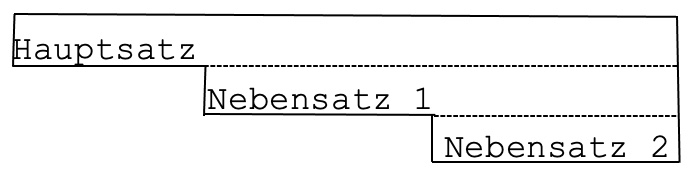
\includegraphics[width=7cm]{figures/Satzbild_Korpora.jpeg}
    %% Abbildung 


\centering{
	\noindent\resizebox{\textwidth}{!}{
		
		\begin{tabular}{ p{4cm} p{4cm} p{4cm} | }
			
			\hline 
			\multicolumn{1}{ | l }{\makecell[l]{\small\textcolor{gray}{Hauptsatz}}} && \\ \cline{1-1} \sbdashline{2-3}
			
			& \multicolumn{1}{ | l }{\makecell[l]{\small\textcolor{gray}{Nebensatz 1}}} &  \\ \cline{2-2} \sbdashline{3-3}
			
			& & \multicolumn{1}{ | l | }{\makecell[l]{\small\textcolor{gray}{Nebensatz 2}}}  \\ \cline{3-3}
			
		\end{tabular}
	}
}




    \caption{Satzbild zu (\ref{ea:EisenbergSatz})}
    \label{Abb:Satzbild_Korpora}
\end{figure}

Die Satzgliedanalyse beginnt auf der Hauptsatzebene. Zuerst muss das Hauptprädikat als hierarchisch oberste Einheit bestimmt werden. In unserem Satz ist \textit{verfügen} das Prädikat in der Lesart von \gq{etwas besitzen und verwenden können}. Nun bestimmen wir die Valenz des Prädikats. Es ist zweiwertig. Die erste Ergänzung wird durch die Nominativ-NP \textit{wir} in Subjektfunktion realisiert. Die zweite Ergänzung wird als PP mit \textit{über} in Funktion eines Präpositionalobjekts ausgedrückt. Wir haben festgestellt, dass der erste Nebensatz in die NP \textit{riesige elektronische Korpora} eingebettet ist. Diese wiederum ist Teil der PP, also: \textit{über riesige elektronische Korpora, an denen wir genau sehen können}. Den zweiten Nebensatz haben wir als Teil des ersten Nebensatzes bestimmt. Die PP ist also äußerst komplex. Mit beiden Nebensätzen zusammen fungiert sie auf der Hauptsatzebene als Präpositionalobjekt des Prädikats \textit{verfügen}. 

Hierfür sprechen auch die Satzgliedtests: Die komplexe PP ist auf oberster Ebene als Ganze pronominalisierbar (\ref{ea:PPdarüber}), erfragbar (\ref{ex:PPworüber}) und voranstellbar (\ref{ex:PPvorangestellt}).

\ea \label{ea:SGTests}
\ea \label{ea:PPdarüber} Wir verfügen heute [darüber].
\ex \label{ex:PPworüber} [Worüber] verfügen wir heute?
\ex \label{ex:PPvorangestellt} [Über riesige elektronische Korpora, an denen wir genau sehen können, an welchen Punkten die Journalisten ihren Schreibgebrauch verändert haben], verfügen wir heute.
\z 
\z 

Neben den primären Satzgliedern Subjekt und Präpositionalobjekt bezieht sich die Adverbphrase \textit{heute} ebenfalls direkt auf die Hauptsatzebene und ist daher als Adverbial das dritte Satzglied des Hauptsatzes. 

Die Analyse\is{Satzgliedanalyse im Tabellenformat} des Hauptsatzes ausgehend vom Hauptprädikat wird in der ersten Spalte der Tabelle~\ref{tab:SGATabelle} festgehalten.\footnote{Möglich wäre es auch, wie \citet{Welke2007} die Ebene des Gesamtsatzes in der letzten Spalte zu analysieren quasi als Endprodukt des Strukturaufbaus. Wir gehen umgekehrt vor und stellen wie \citet[80--81]{Musan2021_SGA} die Zerlegung der Gesamtstruktur in den Vordergrund.} Zwar braucht diese Art der (vertikalen) Darstellung in einer Tabelle mehr Platz als die gewöhnliche horizontale Schreibweise. Aber sie bietet zwei Vorteile, die für eine syntaktische Analyse wesentlich sind: Sie ist übersichtlich und sie erlaubt es, die Einbettung durch die Wahl der jeweiligen Spalte darzustellen. Die hierfür benötigte Anzahl der Spalten entspricht der Anzahl der Ebenen im Satzbild. Wenn das Satzbild in Abbildung~\ref{Abb:Satzbild_Korpora} um 90 Grad nach links gedreht wird, dann entsprechen die drei Ebenen den drei Tabellenspalten in der Tabelle~\ref{tab:SGATabelle}.  

\begin{table}
  \centering
  \begin{tabular}{l|l|l|l}
    %\lsptoprule
      & Hauptsatz & 1. Nebensatzebene & 2. Nebensatzebene\\
    \hline
    \textit{Wir} & Subjekt & & \\ \cline{2-2}
    \textit{verfügen} & Prädikat & & \\ \cline{2-2}
    \textit{heute} & Adverbial & & \\ \cline{2-2}
    \textit{über} & \multirow{19}{*}{Präpositional-} & &\\ 
    \textit{riesige} & \multirow{19}{*}{objekt}  & &\\ 
    \textit{elektronische} & & &\\ 
    \textit{Korpora,} & & &\\ \cline{3-3}
    \textit{an} & & \multirow{2}{*}{Adverbial} &\\
    \textit{denen} & & &\\  \cline{3-3}  
    \textit{wir} & & Subjekt &\\  \cline{3-3} 
    \textit{genau} &  & Adverbial & \\ \cline{3-3}  
    \textit{sehen} & & \multirow{2}{*}{Prädikat} & \\   
    \textit{können,} & & &\\ \cline{3-4} 
    \textit{an} & & \multirow{9}{*}{Satzobjekt} & \multirow{3}{*}{Adverbial} \\ 
    \textit{welchen} & & & \\ 
    \textit{Punkten} & & &\\ \cline{4-4}
    \textit{die} & & &\multirow{2}{*}{Subjekt} \\ 
    \textit{Journalisten} & & \\ \cline{4-4}
    \textit{ihren} & & & \multirow{2}{*}{Akkusativobjekt}\\ 
    \textit{Sprachgebrauch} & &\\ \cline{4-4} 
    \textit{verändert} & & & \multirow{2}{*}{Prädikat}\\ 
    \textit{haben.} & & &\\
    \hline
    %\lspbottomrule
  \end{tabular}
  \caption{Satzgliedanalyse im Tabellenformat}
  \label{tab:SGATabelle}
\end{table}

Erst in weiteren Tabellenspalten analysieren wir den internen Aufbau des komplexen Präpositionalobjekts. So wie kleinere Kisten aus größeren Kisten zum Vorschein kommen können, so gehen wir mit dem Instrumentarium der Satzgliedanalyse schrittweise in die vom Haupträdikat weiter entfernten, von Nebenprädikaten abhängigen (tiefer eingebetteten) Satzglieder. Die bereits auf der obersten Ebene (linke Spalte) analysierten Satzglieder sind \gq{abgearbeitet}. Die Felder in den weiteren Tabellenspalten bleiben leer.

Direkten\is{Nebensatz!Einbettung} Bezug zur Hauptsatzebene hat der erste Nebensatz. Denn er ist Teil des Präpositionalobjekts. Diese Nähe erfassen wir in der Tabelle dadurch, dass wir den ersten Nebensatz in der zweiten Spalte analysieren. Dazu gehen wir wieder vom Prädikat aus. Dieses steht am Ende und lautet \textit{sehen können}. Es ist zweiwertig. Die erste Ergänzung wird durch die Nominativ-NP \textit{wir} in Subjektfunktion ausgedrückt und die zweite Ergänzung, das Gesehene, durch den zweiten Nebensatz in Objektfunktion, daher Satzobjekt. Dessen interne Struktur spielt auf der zweiten Ebene (in der zweiten Spalte) keine Rolle. Neben Subjekt und Objekt gibt es zwei Adverbiale, nämlich das Lokaladverbial \textit{an denen} und das Modaladverbial \textit{genau}. Wenn wir aus dem ersten (einbettenden) Nebensatz einen Hauptsatz bilden, können wir insbesondere die Voranstellbarkeit der fraglichen Satzglieder testen.

\ea \label{ea:NeSaSatzglied}
\ea \label{ea:PPTop} [An ihnen] können wir genau sehen, an welchen Punkten die Journalisten ihren Sprachgebrauch in den letzten Jahren verändert haben.
\ex \label{ex:SubjTop} [Wir] können an ihnen genau sehen, an welchen Punkten die Journalisten ihren Sprachgebrauch in den letzten Jahren verändert haben.
\ex \label{ex:AdvTop} [Genau] können wir an ihnen sehen, an welchen Punkten die Journalisten ihren Sprachgebrauch in den letzten Jahren verändert haben.
\ex \label{ex:NeSaTop} [An welchen Punkten die Journalisten ihren Sprachgebrauch in den letzten Jahren verändert haben], können wir an ihnen genau sehen.
\z 
\z 

Erst\is{Nebensatz!Einbettung} auf der letzten (dem Hauptprädikat und damit Hauptsatz) entferntesten Ebene wird die interne Struktur des zweiten Nebensatzes analysiert. Da er sich auf den ersten Nebensatz bezieht, den wir in der zweiten Spalte analysiert haben, müssen wir seine Glieder in der dritten Spalte (2. Nebensatzebene) bestimmen. Auch hier beginnen wir wieder mit dem Prädikat \textit{verändert haben}. Es ist zweiwertig. Die erste Ergänzung wird durch die Nominativ-NP \textit{die Journalisten} mit Subjektfunktion realisiert, die zweite durch die Akkusativ-NP \textit{ihren Sprachgebrauch} mit Objektfunktion. Die PP \textit{an welchen Punkten} ist als Adverbial hinzugefügt. Es handelt sich im weiteren Sinne um eine Bestimmung des Ortes.   


Damit ist der Satz (\ref{ea:EisenbergSatz}) schrittweise in seine Glieder zerlegt, ebenenspezifisch vom Haupt- zu den Nebenprädikaten. Um komplexe Sätze geht es im Abschnitt~\ref{section:komplexeSätze}. 

Nach der Satzgliedanalyse bestimmen wir die Attribute und ihre Köpfe (Bezugswörter) außerhalb der Tabelle.\footnote{\citet[1, 125]{Welke2007} kennzeichnet Attribute innerhalb der Tabelle durch Pfeile, die auf das Bezugswort gerichtet sind. \citet[68]{Musan2021_SGA} kennzeichnet Attributbeziehungen auch innerhalb der Tabelle durch Boxen innerhalb der Satzglieder. Wir unterscheiden strikt zwischen Satzgliedstrukturen innerhalb der Tabelle und Attributbeziehungen außerhalb.} Auch hier gehen wir ebenenspezifisch (nach Spalten) vor. Auf der ersten Ebene ist die NP innerhalb des Präpositionalobjektes komplex. Zuerst bezieht sich das Adjektivattribut \textit{elektronische} auf den nominalen Kopf \textit{Korpora}. Auf diesen Komplex bezieht sich im nächsten Schritt das Adjektivattribut \textit{riesige}. Der so gebildete nominale Komplex \textit{riesige elektronische Korpora} wird weiter bestimmt durch das Nebensatzattribut \textit{an denen wir genau sehen können, an welchen Punkten die Journalisten ihren Sprachgebrauch verändert haben}. Die Reihenfolge, in der sich die Attribute auf den Kopf beziehen, wird formal nicht angezeigt. Dies geschieht primär nach semantischen Gesichtspunkten. Auf der ersten Nebensatzebene gibt es keine Attribute. Auf der zweiten Nebensatzebene kann der Possessivartikel \textit{ihren} auch als Attribut zum nominalen Kopf \textit{Sprachgebrauch} bestimmt werden. Dann hat er eine Doppelfunktion: als Artikel ist er grammatischer Bestandteil der NP (vgl. Abschnitt~\ref{section:NP}) und semantisch wird er als Merkmal auf das vom Nomen Bezeichnete übertragen.     


\section{Prädikat}\label{subsection:komplexe Prädikate I}

Das Verb bzw. der Verbkomplex bildet aufgrund seiner Valenz das strukturelle Zentrum des Satzes. Die Funktion, auf Satzebene Leerstellen für Ergänzungen zu eröffnen, bezeichnet man in der Satzgliedanalyse als Prädikat. Eine Wortgruppe ist nur dann ein Satzglied, wenn sie eine direkte Beziehung zum Prädikat hat, sei es als valenzsättigender Ausdruck (Ergänzung) oder als zusätzlicher spezifizierender oder kommentierender Ausdruck. \citet[203]{Christ2017} beschreibt das Prädikat mit dem Bild eines Marionettenspielers, \gqq{der die Satzglieder in der Hand hält}. 

Allerdings lehnt \citet[195--199]{Christ2017} den Prädikatsbegriff als solchen für die Schule ab und spricht nur vom Verb bzw. vom Verbkomplex. Wir halten erstens die terminologische Unterscheidung zwischen Wortart (Verb) und Funktion (Prädikat) für sinnvoll. Zweitens ist zu berücksichtigen, dass Prädikate auch nicht-verbale Bestandteile enthalten können, \zB sogenannte Verbpartikeln wie \textit{an} in \textit{Er ruft sie morgen an} (vgl. Abschnitt~\ref{subsection:VPartikeln}), inkorporierte Substantive wie \textit{Karten} in \textit{Sie spielt Karten} oder Präpositionalphrasen wie \textit{in Brand} in \textit{Er setzt das Haus in Brand} (vgl. Abschnitt~\ref{subsection:IdiomeNVGFVG}).
 
Durch die Spitzenstellung ist das Prädikat\is{Prädikat} kein Satzglied unter anderen Satzgliedern, sondern aufgrund seiner Valenz, und damit seiner Rektion und seiner prädikativen Kraft, das konstituierende Zentrum des Satzes.\footnote{\citet[71]{Boettcher2009EinfSatz}, \citet[195--204]{Christ2017} und \citet[44]{PittnerBerman2021} zählen das Prädikat (bzw. das Verb) nicht zu den Satzgliedern, da es sich bezüglich der Tests anders als die übrigen Satzglieder verhält: es ist nicht verschiebbar, nicht erfragbar und auch nicht pronominalisierbar. Für \citet[34, 38]{Elst_Habermann_SynAn} nimmt das Prädikat die regierende Spitzenstellung im Satz ein. Als Satzglied bezeichnen sie wie auch \citet[35]{Woellstein_Heilmann_Vikner_2006} und \citet[146]{OehlSeiler2013} nur die Wörter und Wortgruppen, die unmittelbar vom Prädikat abhängen. \citet[45]{Agel2017} zählt das Prädikat zu den Satzgliedern, stellt es jedoch an deren Spitze. Er verortet es in einer konzentrischen Kreisdarstellung der Satzglieder im Zentrum.}

In der\is{Prädikat!mehrteilig} Satzgliedanalyse geht es nicht um die internen Rektionsverhältnisse innerhalb eines komplexen Prädikats (vgl. Abschnitt~\ref{section:RegierteVerben}). Es geht einfach darum, zu erkennen, welche Teile zum Prädikat gehören bzw. das Prädikat bilden. 

\begin{Definition}{Prädikat}
    
\noindent Als Prädikat wird die Funktion des Verbs oder Verbalkomplexes (auch mit nicht verbalen Bestandteilen) bezeichnet, Leerstellen zu eröffnen, deren Sättigung zu minimal vollständigen Sätzen führt. Das Prädikat ist das satzbildende Zentrum.    
\end{Definition}

Die Position des Prädikats bzw. seiner Bestandteile im Satz haben wir in Kapitel \ref{chapter:Feldermodell} mithilfe des Feldermodells (LSK, RSK) beschrieben. Bei der Analyse im\is{Satzgliedanalyse im Tabellenformat} Tabellenformat bezeichnen wir sowohl den finiten Prädikatsteil als auch den infiniten als Prädikat. Dies zeigen wir in Tabelle~\ref{tab:komplPrädikate}.

\begin{table}
  \centering
  \begin{tabular}{l|l}
   % \lsptoprule
      & Hauptsatz \\
    \hline
    \textit{Anna} & Subjekt  \\ \cline{2-2}
    \textit{wird} & Prädikat  \\ \cline{2-2}
    \textit{das} & \multirow{2}{*}{Akkusativobjekt} \\ 
    \textit{Buch} &  \\ \cline{2-2}  
    \textit{gelesen} &  \multirow{3}{*}{Prädikat} \\  
    \textit{haben} &  \\
    \textit{müssen.} &  \\ 
    \hline 
   % \lspbottomrule
  \end{tabular}
  \caption{Komplexe Prädikate im Tabellenformat}
  \label{tab:komplPrädikate}
\end{table}

Prädikate sind das strukturelle und semantische Zentrum von Sätzen. Sie weisen ihren Ergänzungen eine bestimmte Form zu und den von ihnen bezeichneten Entitäten Rollen in einem Szenario, was wir in Abschnitt~\ref{section:KonzeptVerbvalenz} als Prädikation (vgl. Definition~\ref{Def_Prädikation}) bezeichnet haben. Als Szenariotypen haben wir Handlungen, Tätigkeiten, Vorgänge und Zustände (vgl. Abschnitt~\ref{subsection:Verbklassen}) unterschieden.


\section{Satzglieder}\label{section:Satzglieder}

Als Satzglied\is{Satzglied} bezeichnet man ein Wort oder eine Wortgruppe, die als unmittelbare Konstituente des Satzes eine direkte Beziehung zum Prädikat hat. In diesem Sinne beschreibt \citet[80]{Engel2009} die Satzglieder als \gqq{Satelliten} des Prädikats. 

Primär geht es um die Satzglieder, die das Prädikat aufgrund seiner Valenz (vgl. Kapitel~\ref{chapter:Valenz}) fordert: das Subjekt (vgl. Abschnitt~\ref{subsection:Subjekt}) und die Objekte: Das Akkusativobjekt (vgl. Abschnitt~\ref{subsection:Akkusativobj}), das Dativobjekt (vgl. Abschnitt~\ref{subsection:Datobj}), relikthaft das Genitivobjekt (vgl. Abschnitt~\ref{subsection:Genitivobjekt}) und das Präpositionalobjekt (vgl. Abschnitt~\ref{subsection:Pobj}). In einer erweiterten Version nach \citet[1]{Welke2007} zählen wir auch das \textit{Direktivum} (vgl. Abschnitt~\ref{subsection:Direktivum}) dazu. Sie bilden zusammen mit dem Prädikat das Grundgerüst von Sätzen. Deshalb bezeichnet man sie seit \citet[92--93]{Helbig1978sekSG} auch als \textit{primäre} Satzglieder. \citet[47]{Agel2017} nennt sie \textit{statische} Satzglieder. In Abschnitt~\ref{subsection:Valenzdynamik} sind wir auf die Erhöhung der Grundvalenz als Valenzdynamik eingegangen. Diese führt zu \textit{dynamischen} Satzgliedern, auf die wir in jedem Abschnitt verweisen.

Auf die wenigen Verben, die wie \textit{geruhen} ausschließlich satzwertige Ergänzungen (Verbativergänzungen) zu sich nehmen, haben wir in Abschnitt~\ref{section:KonzeptVerbvalenz} hingewiesen. Auf ihre Thematisierung als Verbativobjekte in der Satzanalyse verzichten wir.  
      

Zu den Satzgliedern zählen auch die spezifizierenden Erweiterungen des Verbszenarios durch Angaben (vgl. Abschnitt~\ref{subsection:EvsA}). Sie beziehen sich auf das Prädikat oder den Satz, ohne in der Verbvalenz verankert zu sein. Diese Funktion bezeichnet man als Adverbial (vgl. Abschnitt~\ref{subsection:Adverbial}). Eine Untergruppe bilden die kommentierenden Angaben wie \textit{leider}, die wir als Kommentaradverbiale (vgl. Abschnitt~\ref{subsubsection:Kommentaradverbial}) bestimmen. Da Adverbiale nicht durch die Valenz des Prädikats zum Grundgerüst des Satzes gehören, sondern dieses ausbauen, bezeichnet man sie als \textit{sekundäre} Satzglieder.  

\begin{Definition}{Satzglieder: primäre und sekundäre}
    
\noindent Satzglieder sind Konstituenten (ein Wort oder eine Wortgruppe), die in direkter Beziehung zum Prädikat stehen. Ihr jeweiliger Bezug zum Prädikat oder Satz wird durch Satzgliedfunktionen erfasst. Primäre Satzglieder sättigen Leerstellen der Valenz des Prädikats. Sekundäre Satzglieder sättigen keine Valenzanforderungen des Prädikats.      
\end{Definition}


In Abschnitt~\ref{subsection:freiePräd} geht es um \textit{freie Prädikative} als besondere sekundäre Satzglieder. 

Satzglieder\is{Satzglied} bilden die unmittelbaren Konstituenten von Sätzen. Die Tests zu ihrer Ermittlung haben wir in Kapitel \ref{chap:Konstituenz} vorgestellt: Satzglieder können wir ersetzen, insbesondere durch Pro-Formen und Fragewörter, sie sind innerhalb des Mittelfelds umstellbar und können allein das Vorfeld besetzen. 



\subsection{Subjekt}\label{subsection:Subjekt}

Als\is{Subjekt} Subjekt bezeichnet man die Funktion einer NP im Nominativ oder eines Äquivalents, das die erste verbale Ergänzung realisiert. Das Subjekt korrespondiert formal als einziges Satzglied mit dem finiten Teil des Prädikats.\footnote{Aus anderer Perspektive könnte man auch wie \citet[95, 126]{Tesniere1980deutsch} sagen, dass das Subjekt zweigliedrig ist, da es als NP \textit{und} in der Verbendung ausgedrückt wird. Bei der Verbindung handelt es sich historisch um eigenständige Subjektpronomen, die vom Verb \gqq{einverleibt} wurden. Insofern beruht die formale Korrespondenz auf Inkorporation des Subjekts und zusätzlicher Subjektrealisierung auf syntaktischer Ebene. Zur (sprachvergleichenden) Vertiefung empfehlen wir \citet{Agel1995}.} 

Handelt es\is{Subjekt-Finitum-Kongruenz} sich beim Subjekt um Personalpronomen, so kongruiert die Verbform in Person und Numerus mit dem Subjekt. In (\ref{ea:PersPrnKorrespondenz}) kongruiert die Endung des Verbs einmal mit der ersten Person Singular \textit{ich} und einmal mit der ersten Person Plural \textit{wir}. 

\ea \label{ea:PersPrnKorrespondenz} ich geh-e, wir geh-en 
\z 

Handelt es sich um eine substantivische NP wie in (\ref{ea:SubstKorrespondenz}), dann kongruiert der finite Teil des Prädikats nur mit dem Numerus der NP. Da Substantive nicht über die Kategorie Person verfügen, wird als Grundregel beim Verb die Form der dritten Person gewählt. Deshalb schlägt \citet[312]{Eisenberg2020_Satz} anstelle des Kongruenz- den \textit{Korrespondenz}-Begriff vor. Die Korrespondenz zwischen dem Nomen und der Verbendung der dritten Person ist motiviert, da entsprechende Nomen durch Pronomen der dritten Person Singular oder Plural ersetzt werden können (\ref{ex:3PersKorrespondenz}). 

\ea \label{ea:SubjPrädkorrespondenz}
\ea \label{ea:SubstKorrespondenz} der Mann geh-t, die Männer geh-en
\ex \label{ex:3PersKorrespondenz} er geh-t, sie geh-en
\z 
\z 

Außer NPs im Nominativ (\ref{ea:NomNPSubjekt}) werden auch äquivalente\is{Subjekt!Satzsubjekt} Nebensätze (\ref{ex:NeSaSubjekt}) oder nebensatzähnliche Infinitivgruppen (\ref{ex:InfSubj}) als Subjekt gebraucht. Das finite Verb steht bei einem oder mehreren koordinierten Nebensätzen (\ref{ex:2NeSaSubjekte}) grundsätzlich in der dritten Person Singular.  

\ea \label{ea:Subjektäquivalente}
\ea \label{ea:NomNPSubjekt} \textit{Dein Besuch} freut mich.
\ex \label{ex:NeSaSubjekt} \textit{Dass du mich besuchst}, freut mich.
\ex \label{ex:InfSubj} \textit{Dich zu sehen}, freut mich.
\ex \label{ex:2NeSaSubjekte} \textit{Dich zu sehen und mit dir zu sprechen}, freut (*freuen) mich.    
\z 
\z 

Diese Äquivalente sind typisch für Verben wie \textit{freuen} oder \textit{schmerzen}, die psychische und physische Vorgänge oder Zustände ausdrücken. Die durch die Nebensätze bezeichneten Ereignisse lösen physische und psychische Vorgänge oder Zustände aus oder beinhalten sie.  

In\is{Subjekt!Satzsubjekt} der Satzanalyse im Tabellenformat wird im Falle von Nebensätzen und nebensatzähnlichen Konstruktionen die interne Struktur des Nebensatzes auf einer tieferen Analyse-Ebene in Form einer weiteren Spalte aufgelöst. Dies wird in Tabelle~\ref{tab:SubjNS} gezeigt.\footnote{Subjunktionen wie \textit{dass} können in der Satzgliedanalyse nicht bestimmt werden, weil sie keine Satzglieder, aber auch keine Attribute sind. Deshalb wird in der Ebene, auf der durch sie eingeleitete Nebensätze analysiert werden, ein Strich gesetzt.} 


\begin{table}
  \centering
  \begin{tabular}{l|l|l}
   % \lsptoprule
      & Hauptsatz & 1. Nebensatzebene \\
    \hline
    \textit{Dass} & \multirow{4}{*}{Subjekt} & -- \\ \cline{3-3}
    \textit{du} & & Subjekt \\ \cline{3-3}
    \textit{mich} & & Akkusativobjekt \\ \cline{3-3}
    \textit{besuchst,} & & Prädikat  \\ \cline{2-3}
    \textit{freut} & Prädikat &  \\ \cline{2-2} 
    \textit{mich.} & Akkusativobjekt &  \\  
    \hline 
   % \lspbottomrule
  \end{tabular}
  \caption{Auflösung des Subjekt-Nebensatzes}
  \label{tab:SubjNS}
\end{table}

Als Realisierung der ersten verbalen Ergänzung bezeichnet das Subjekt in Abhängigkeit von der Verbbedeutung (vgl. Abschnitt~\ref{subsection:Verbklassen}) den Träger einer Handlung (\ref{ea:Handlungsträger}), einer Tätigkeit (\ref{ex:Tätigkeitsträger}), eines Vorgangs (\ref{ex:Vorgangsträger}) oder eines Zustands (\ref{ex:Zustandsträger}).

\ea \label{ea:Subjektrollen}
\ea \label{ea:Handlungsträger} \textit{Der Bauer} pflügt seinen Acker.
\ex \label{ex:Tätigkeitsträger} \textit{Sie} arbeitet.
\ex \label{ex:Vorgangsträger} \textit{Der alte Mann} zittert.
\ex \label{ex:Zustandsträger} \textit{Wer} sitzt im Garten?
\z 
\z 

Typischerweise handelt es sich beim Subjekt um den Ausdruck der ersten verbalen Ergänzung, also um den im Verb angelegten Ausgangspunkt eines Szenarios. Diesen bezeichnet \citet[139]{Erben1980} als \gqq{Ansatzstelle}. Es geht um die valenzielle Anlage einer Ereignisdarstellung als schrittweise In-Blick-Nahme einer Szene.\footnote{Explizit entwickelt \citet[211--212]{Welke1988}, \citet[111]{Welke2005} auf der Grundlage der kognitiven Grammatik nach \citet{Langacker1987} ein perspektivisches Rollenkonzept. Auch \citet[308--309]{Eisenberg2020_Satz} geht von perspektivischer Ausgezeichnetheit und daraus folgenden prototypischen Subjekteigenschaften aus.} Bei aktivischen finiten Verbformen realisiert das Subjekt normalerweise die erste und das Objekt die zweite und/oder dritte Ergänzung. Diese angelegte Reihenfolge (Perspektive) kann durch einfache Umstellungen (\textit{ihn habe ich gesehen} statt \textit{ich habe ihn gesehen}) sowie kategorial \zB durch das Passiv (\textit{er wurde gesehen}) geändert werden.\footnote{Wenn aufgrund uneindeutiger oder fehlender Kasusmarkierung unklar ist, welches Satzglied Subjekt und welches Objekt ist, dann verstehen wir das zuerst realisierte Satzglied als Subjekt und die folgenden als Objekt (\textit{Paul liebt Anna}). Rein grammatisch ist unklar, \textit{wer} \textit{wen} liebt. Grammatisch klar ist aber, dass, wenn eine NP als Subjekt interpretiert wird, die andere dann als Objekt verstanden werden muss.} Auf die Veränderung der angelegten Perspektive durch das Passiv kommen wir im Abschnitt~\ref{subsection:Passiv} zurück.

Aus der Realisierung der ersten (perspektivisch ausgezeichneten) Ergänzung durch das Subjekt können typische, aber nicht notwendige Eigenschaften folgen. Da wir mit indoeuropäischen Sprachen Ereignisse so weit wie möglich aus Handlungsperspektive darstellen (vgl. Abschnitt~\ref{subsection:Verbklassen}) bezeichnen die Subjekt-NPs häufig belebte, handelnde oder verantwortliche Entitäten. In der Kommunikation nutzen wir, nach Auszählung einer Stichprobe durch \citet[44]{Engel1972}, in ca. 60\% das Subjekt tatsächlich als zuerst realisierte Ergänzung, das heißt als Anknüpfungs- bzw. Ansatzpunkt, unter dem der Rezipient neue Informationen verbuchen kann.\footnote{Hier geht es um die Stellung des Subjekts vor anderen valenzgeforderten Satzgliedern. Das muss nicht die Stellung im Vorfeld (vgl. Abschnitt~\ref{subsection:Vorfeld}) sein. Auch im Mittelfeld steht typischerweise das Subjekt vor den Objekten (\ref{ea:Subj_1_MF}). Das gilt für Verbletzt- (\ref{ex:Subj_Vend}) und für Verberstsätze (\ref{ex:Subj_Verst}). 

\ea \label{ea:Subj_1_MF} Morgen pflügt \textit{der Bauer} den Acker.
\ex \label{ex:Subj_Vend} dass \textit{der Bauer} morgen den Acker pflügt
\ex \label{ex:Subj_Verst} Pflügt \textit{der Bauer} morgen den Acker? 
\z

In Abschnitt~\ref{subsection:Vorfeld} haben wir gezeigt, dass viele andere Stellungen im Mittelfeld möglich sind. Um Stellungspräferenzen ging es in Exkurs~\ref{Exkurs:Stellung_MF}.}


\begin{Definition}{Subjekt}
    
\noindent \noindent Das Subjekt\is{Subjekt} ist eine NP im Nominativ oder ein äquivalenter satzförmiger Ausdruck, der typischerweise die erste in der Valenz des Prädikats angelegte Leerstelle sättigt. Das Subjekt kongruiert mit dem finiten Verb des Prädikats im Numerus und bei Pronomen auch in der Person.   
\end{Definition}


Witterungsverben wie\is{Subjekt!formales} \textit{regnen} oder \textit{stürmen} verfügen nur über das syntaktische Subjekt\is{es@\textit{es}!formales Subjekt} \textit{es}. Dem Subjekt wird durch das Prädikat keine semantische Rolle zugewiesen (es gibt keine \gq{regnende} Entität). Ausdrücke wie (\ref{ea:es regnet}) verweisen auf ein entsprechendes Geschehen.

\ea \label{ea:es regnet} Es regnet/stürmt/schneit/gewittert \ldots{} 
\z 

Ausgehend von der Grundvalenz aktivischer finiter Verben ist im Deutschen der Ausdruck des Subjekts als Satzglied obligatorisch. Hierin liegt ein Unterschied zu sogenannten \textit{pro-drop}-Sprachen (pronoun dropping) wie \zB dem Spanischen, wo das Subjektpronomen nicht als Satzglied, sondern allein durch die Verbflexion realisiert werden kann. So entspricht dem deutschen Satz \textit{ich liebe dich} auf Spanisch \textit{te amo}, oberflächlich wörtlich also \textit{dich liebe}. Das Subjekt fehlt aber nicht, sondern es ist in der Flexionsform der ersten Person Singular Präsens Indikativ Aktiv \textit{amo} durch -\textit{o} ausgedrückt. Das wird in (\ref{ea:SpanischProDrop}) dargestellt.

\ea \label{ea:SpanischProDrop}
\gll Te am-o. \\
     2SG.AKK lieb-1SG.PRS.IND.AKT\\
 \glt ‘Ich liebe dich.’    
\z 

Ähnlich implizit\is{Subjektlosigkeit} ist das Subjekt in der Standardschriftlichkeit\footnote{In der Umgangssprache ist der sogenannte Telegrammstil wie \textit{Komme später} in einer SMS oder \textit{Erinner' mich nich}(\textit{t}) im Dialog durchaus üblich.} nur beim Imperativ der 2. Person Singular (\ref{ea:Imp2PSgl}) und Plural (\ref{ex:Imp2PPl}), also bezüglich des Adressaten. Dieser ist in der Kommunikationssituation präsent. Seine formale Kennzeichnung findet nicht syntaktisch, sondern morphologisch in der Verbform statt.

\ea \label{ea:Imperativ2P}
\ea \label{ea:Imp2PSgl} Komm!
\ex \label{ex:Imp2PPl} Kommt!
\z 
\z 

Subjektlose Sätze sind im sogenannten unpersönlichen Passiv wie in (\ref{ea:OhneSubjektPassiv}) zu finden. Hierum wird es in Abschnitt~\ref{subsection:Passiv} gehen. 

\ea \label{ea:OhneSubjektPassiv}
\ea \label{ea:UnpPassiv} In der Kirche wird gebetet und gesungen.
\ex \label{ex:UnpPassivImp} Jetzt wird aber geschlafen!
\z 
\z 


In den Abschnitten~\ref{subsubsection:TestFOSP} und \ref{section:VP} wurde auf infinite VPs wie \textit{ein Lied singen} hingewiesen. Sie haben kein syntaktisches Subjekt. Dennoch verstehen wir es über das Subjekt (\textit{Anna versucht zu schlafen}) oder über das Objekt (\textit{Anna bittet Paul, ihr zu helfen}) des übergeordneten Satzes mit. 

Auf\is{Subjektlosigkeit} archaische Valenzen ohne Nominativ-NP haben wir in Abschnitt~\ref{subsubsection:TestFOSP} hingewiesen. Es gibt wenige Verben, deren erste Ergänzung im Akkusativ (\ref{ea:michfriert}) oder im Dativ (\ref{ex:mir graut}) ausgedrückt wird. 

\ea \label{ea:KeinSubjekt}
\ea \label{ea:michfriert} Mich friert. (versus: Ich friere)
\ex \label{ex:mir graut} Mir/Mich gruselt vor der Prüfung. (versus: Ich grusle mich vor der Prüfung)
\z 
\z 

In diesen Sätzen gibt es kein grammatisches Subjekt.\footnote{In Anlehnung an \citet[124]{Paul1880} wird hier auch von einem \textit{psychologischen} im Gegensatz zum grammatischen Subjekt gesprochen. Dabei handelt es sich um die typischerweise zuerst realisierte Ergänzung als Ansatzpunkt der Ereignisdarstellung.}


\subsection{Akkusativobjekt}\label{subsection:Akkusativobj}

Durch Objekte werden die weiteren Ergänzungen des Verbs realisiert. Der Prototyp des Objekts ist im Deutschen eine NP im Akkusativ, das\is{Akkusativobjekt} Akkusativobjekt. Die von diesem bezeichnete Entität, die typischerweise der Zielpunkt des Szenarios ist, steht dem Referenten des Subjekts als Ausgangspunkt gegenüber. Anstelle der jeweiligen Referenten sprechen wir im Folgenden verkürzt auch einfach vom Subjekt und Objekt.  

Verben mit Akkusativobjekt nennt man\is{Verbklassen!transitiv} \textit{transitiv}. Die Handlung des Subjekts geht direkt auf das Objekt über (lat. \textit{transire}). Deshalb bezeichnet man das Akkusativobjekt auch als \textit{direktes Objekt}. Die grundsätzliche semantische Leistung ist die Kodierung eines Szenariobeteiligten als \textit{Handlungsgegenstand} oder \textit{Patiens} (vgl. Abschnitt~\ref{subsection:Verbklassen}).
 
Die Funktion des Akkusativobjekts können auch äquivalente\is{Akkusativobjekt!Satzobjekt} Nebensätze (\ref{ea:dassObjektsatz}) und Infinitivgruppen (\ref{ex:InfObj}) übernehmen.

\ea \label{ea:AkkobjÄquivalente}
\ea \label{ea:dassObjektsatz} Er sagt, \textit{dass er später kommt}.
\ex \label{ex:InfObj} Er sagt, \textit{später zu kommen}.
\z 
\z 

Dies ist insbesondere bei den Verben des Sagens sowie bei den Verben des Fühlens und Denkens der Fall. Aufgrund ihrer Bedeutung bezieht sich die zweite Ergänzung häufig auf Aussagen und Sachverhalte, die wir durch Sätze beschreiben. Bei diesen Verben kann anstelle eines \textit{dass}-Nebensatzes (\ref{ea:dassObjektsatz}) auch ein abhängiger Verbzweitsatz gebraucht werden (\ref{ea:Verbzweitsatz}), der die Funktion des erwartbaren Akkusativobjekts erfüllt. In Abschnitt~\ref{subsection:FormFktNeSa} kommen wir unter dem Stichwort \textit{verkappter Nebensatz} auf uneingeleitete Nebensätze zurück. 

\ea \label{ea:Verbzweitsatz} Er sagt, \textit{er komme später}.
\z 

Bei den Verben des Fragens, Sagens und (Nicht-)Wissens sowie des Wahrnehmens können die\is{Akkusativobjekt!Satzobjekt} Satzobjekte auch durch \textit{ob} (\ref{ea:obSatz}) oder durch sogenannte W-Fragewörter (\ref{ex:wSatz}) eingeleitet werden.  

\ea \label{ea:andereObjeksätz}
\ea \label{ea:obSatz} Er fragt/weiß (nicht), \textit{ob er helfen soll}.
\ex \label{ex:wSatz} Er sagt, \textit{wann/womit/wobei er helfen wolle}.
\z 
\z 

Diese Nebensätze in Objektfunktion verhalten sich syntaktisch wie Akkusativobjekte, die durch eine NP realisiert werden. Sie sind voranstellbar wie in (\ref{ea:Objsatzvoranstellbar}), pronominalisierbar wie in (\ref{ex:Objsatzpronominalsierbar}), also auch durch ein Fragepronomen erfragbar wie in (\ref{ex:Objsatzerfragbar}).

\ea \label{ea:ObjektsatzwieNP}
\ea \label{ea:Objsatzvoranstellbar} \textit{Ob er helfen soll}, fragt er.
\ex \label{ex:Objsatzpronominalsierbar} Er fragt \textit{das}.
\ex \label{ex:Objsatzerfragbar} \textit{Was} fragt er?
\z 
\z 

So wie wir bei Nebensätzen in Subjektfunktion die interne Struktur in einer tieferen Ebene (weitere Tabellenspalte) analysiert haben, so gehen wir auch bei\is{Akkusativobjekt!Satzobjekt} Satzobjekten vor. Wir könnten sie aufgrund der Äquivalenz mit entsprechenden NPs im Akkusativ als Akkusativobjekt bezeichnen. Da Sätze aber keinen Kasuswert tragen, bezeichnen wir sie als Satzobjekt. Das Format wird in Tabelle~\ref{tab:ObjNS} gezeigt.

\begin{table}
  \centering
  \begin{tabular}{l|l|l}
   % \lsptoprule
     & Hauptsatz & 1. Nebensatzebene \\
    \hline
    \textit{Ob} & \multirow{4}{*}{Satzobjekt} & -- \\ \cline{3-3}
    \textit{er} & & Subjekt \\ \cline{3-3}
    \textit{helfen} & & \multirow{2}{*}{Prädikat} \\ 
    \textit{soll,} & &  \\ \cline{2-3}
    \textit{fragt} & Prädikat &  \\ \cline{2-2} 
    \textit{er.} & Subjekt &  \\  
    \hline 
   % \lspbottomrule
  \end{tabular}
  \caption{Auflösung des Objekt-Nebensatzes}
  \label{tab:ObjNS}
\end{table}



\begin{Definition}{Akkusativobjekt}
    
\noindent Das Akkusativobjekt ist eine NP im Akkusativ oder ein äquivalenter satzförmiger Ausdruck, der typischerweise die zweite oder dritte in der Valenz des Prädikats angelegte Leerstelle sättigt.  
\end{Definition}


Nicht alle Sätze mit Subjekt und Akkusativobjekt beschreiben Handlungen, bei denen das vom Objekt Bezeichnete verändert oder hervorgebracht wird. Von diesem Modell gibt es Abwandlungen. So kann auch die Lage des vom Objekt Bezeichneten verändert werden wie in (\ref{ea:Bewegen}). Oder es wird reine Zielgerichtetheit auf das Objekt (statt dessen Veränderung) wie bei einer ganzen Gruppe von Verben mit der Partikel \textit{an-} ausgedrückt (\ref{ex:anlächeln}). 

\largerpage
\ea \label{ea:Veränderung}
\ea \label{ea:Bewegen} Paul verrückt \textit{den Schrank}.
\ex \label{ex:anlächeln} Sie lächelt \textit{ihn} an. 
\z 
\z 

Die dominierende Handlungsperspektive vom tätigen Subjekt zum behandelten Akkusativobjekt\is{Passiv!mit \textit{werden}} wie in (\ref{ea:Veränderung}) kann grammatisch durch das sogenannte \textit{werden}-Passiv (vgl. Abschnitt~\ref{subsection:Passiv}) wie in (\ref{ea:werden-Passiv}) aufgehoben werden.

\ea \label{ea:werden-Passiv}
\ea \label{ea:verrücktwerden} Der Schrank wird verrückt.
\ex \label{ex:angelächeltwerden} Er wird angelächelt.
\z 
\z 


Im weiteren Sinne fällt unter dieses Darstellungsmodell auch der Ausdruck von Empfindungen. So kann der Stimulus (\textit{deine Nachricht}) in (\ref{ea:etwasfreutmich}) als Freude auslösende Entität als Subjekt und der emotional Betroffene (\textit{mich}) als Objekt ausgedrückt werden. Szenarios dieser Art interpretieren wir als Vorgang, wofür die fehlende Passivierbarkeit (vgl. Abschnitt~\ref{subsection:Passiv}) spricht.

\ea \label{ea:PSYCH}
\ea [] {Deine Nachricht freut \textit{mich}.}\label{ea:etwasfreutmich}
\ex [*] {Ich werde (von deiner Nachricht) gefreut.}\label{ex:*gefreutPassiv}
\z 
\z 

Sprachlich setzen wir aber auch Gefühlsträger als Handelnde in Perspektive und das, worauf sich die Emotion richtet, als Zielgröße im Akkusativ (\ref{ea:ichliebedich}).

\ea \label{ea:ichliebedich} Ich liebe \textit{dich}.
\z 

Die Grenze zwischen Zuständen und Vorgängen ist hier \gqq{unscharf}, wie \citet[144]{Welke2019} schreibt. \citet[252--254]{HopperThompson1980} zeigen, dass mit grammatisch\is{Verbklassen!transitiv} transitiven Verben Sätze gebildet werden, die einen unterschiedlichen Grad an Transitivität (Einwirken des vom Subjekt Bezeichneten auf das vom Objekt Bezeichnete) aufweisen. Äußerst schwach transitiv sind Besitzausdrücke wie in (\ref{ea:Besitz}) oder kognitive Zustände wie in (\ref{ex:PsychZustand}).\footnote{Neben der Semantik der Verben spielt auch die Art der Objektrealisierung eine wesentliche Rolle. Objektausdrücke, die etwas Individuelles bezeichnen wie \textit{einen Baum pflanzen}, führen zu stärkerer Transitivität als indefinite Objektausdrücke im Plural wie \textit{Bäume pflanzen}.}

\ea \label{ea:schwachtransitiv}
\ea \label{ea:Besitz} Anna hat \textit{ein Geheimnis}.
\ex \label{ex:PsychZustand} Paul weiß \textit{das}.
\z 
\z 


Neben der zweigliedrigen Konstellation mit Subjekt und Akkusativobjekt gibt es viele Sätze, in denen ein Akkusativobjekt zusammen mit einem Direktivum (\textit{Ich stelle die Blumen auf den Tisch}) oder mit einem Dativobjekt (\textit{Ich schenke dir einen Blumenstrauß}) vorkommt. Um Dativobjekte geht es in Abschnitt~\ref{subsection:Datobj} und um Direktiva in Abschnitt~\ref{subsection:Direktivum}.

Selten sind heute sogenannte \textit{doppelte} Akkusative, also Verben, die aufgrund ihrer Valenz zwei\is{Akkusativobjekt!doppelt} Objekte im Akkusativ fordern wie in (\ref{ea:lehrendoppAkk}). 

\ea \label{ea:lehrendoppAkk} Eine alte Frau lehrte \textit{ihn} \textit{den Gebrauch der Halszither, die dreizehn Saiten hat}.\footnote{St. Galler Tagblatt, 10.10.1997.}
\z 


In (\ref{ea:lehrendoppAkk}) regiert \textit{lehren} den sogenannten doppelten Akkusativ: \textit{jemand lehrt jemanden etwas}, genauso bei \textit{abfragen}: \textit{jemand fragt jemanden etwas ab} oder bei \textit{kosten}: \textit{etwas kostet jemanden etwas}. 

Seit dem Mittelhochdeutschen besteht hier allerdings die Tendenz, das Objekt, das eine Person bezeichnet, im Dativ auszudrücken (\ref{ea:lehrenDatAkk}), analog zu den Verben, welche den Dativ und den Akkusativ regieren (\ref{ex:beibringen}).\footnote{Diese Tendenz war nach \citet[254]{Paul1919} im 18. Jahrhundert besonders stark und wurde erst später wieder zurückgedrängt. Bildungsbürgerlich gilt dies jedoch als schlechter Ausdruck oder gar als Fehler. Interessant ist hier die einflussreiche Schulgrammatik von \citet[417]{Adelung1782}, der den Dativ aus Analogiegründen vorzieht (!). Hierfür spricht auch, dass beim Passiv das ursprüngliche Akkusativobjekt (\textit{Sein Vater lehrte ihn Mathematik}) nicht zum Subjekt wird (*\textit{Er wird Mathematik gelehrt}), sondern im Dativ ausgedrückt wird (\textit{Ihm wird Mathematik gelehrt}).}

\ea \label{ea:Dat_statt_Doppelakkusativ}
\ea \label{ea:lehrenDatAkk} Godfrey lehrt \textit{ihm} den Umgang mit den modernen Werkzeugen und Waffen.\footnote{Die Schule der Robinsons. In: Wikipedia \url{https://de.wikipedia.org/wiki/Die_Schule_der_Robinsons} (02.10.25).}
\ex \label{ex:beibringen} Er brachte \textit{ihm} den Umgang mit modernen Werkzeugen und Waffen bei.
\z 
\z 

Neben den valenziell geforderten Akkusativobjekten gibt es auch\is{Akkusativobjekt!dynamisch} dynamische Akkusativobjekte (vgl. Abschnitt~\ref{subsection:Valenzdynamik}). Es handelt sich \zB um sogenannte \textit{kognate Objekte} wie in (\ref{ea:KOBelege}). 

\ea \label{ea:KOBelege} Beverly zischte ihr Echsenzischen, Patrick kreischte sein Affenkreischen und Dennis der Hahn gackerte sein Hahnengackern.\footnote{Der Beleg stammt aus \citet[361]{Felfe2018}, der Strukturen mit kognaten Objekten ausführlich beschreibt.}
\z 

Ihr nominaler Kopf ist morphologisch vom Verb abgeleitet (\textit{zischen, das Zischen}) und typischerweise durch Attribute modifiziert (\textit{ein lautes Zischen zischen}) oder via Komposition (\textit{ein Echsenzischen zischen}) näher bestimmt. Als Prädikat kommen hauptsächlich Verben in Frage, deren Bedeutung eine Art Output oder Emission impliziert. Durch die Gesamtkonstruktion wird das Hervorbringen des kognaten Objekts ausgedrückt.

Ebenso kommen\is{Akkusativobjekt!dynamisch} dynamische Akkusativobjekte zusammen mit APs vor, die als Objektsprädikative (vgl. Abschnitt~\ref{subsection:SP und OP}) den Zustand des Akkusativobjekts als Resultat der Handlung beschreiben. Daher spricht man auch von \textit{Resultativkonstruktionen}. Sie sind mit allen agentiven Verben möglich, die auch intransitiv gebraucht werden können. Durch die Gesamtkonstruktion drücken wir aus, dass die Tätigkeit des Subjekts wie in (\ref{ea:RSKBeleg}) \textit{der Hund Hakon hatte gebellt} zu dem Zustand (\textit{wach}) des Akkusativobjekts (\textit{seine Besitzer}) führt.

\ea \label{ea:RSKBeleg} Der Hund Hakon hatte seine Besitzer wach gebellt, als deren Haus im schleswig-holsteinischen Pansdorf brannte.\footnote{die tageszeitung, 28.01.2005. Bei weiterem Interesse an Resultativkonstruktionen verweisen wir auf \citet{Felfe2012}.}
\z 

Sehr ähnlich sehen\is{Akkusativobjekt!dynamisch} kausative Bewegungskonstruktionen aus. Anstelle der AP steht eine direktionale PP, deren syntaktische Funktion wir in Abschnitt~\ref{subsection:Direktivum} als \textit{Direktivum} bezeichnen. Auch in dieser Konstruktion gibt es ein dynamisches Akkusativobjekt. Wie in (\ref{ea:kausBewBeleg}) wird dieses (\textit{ihn}) durch die Tätigkeit des Subjektes (\textit{die Besucherinnen und Besucher im Metropol klatschten}) an den von der PP bezeichneten Ort (\textit{auf die Bühne}) bewegt.

\ea \label{ea:kausBewBeleg} Die Besucherinnen und Besucher im «Metropol» klatschten ihn voller Begeisterung noch mehrmals auf die Bühne.\footnote{St. Galler Tagblatt, 31.10.2015.} 
\z 

In der Satzanalyse werden diese dynamischen Ergänzungen (\textit{den Star auf die Bühne klatschen}) genauso wie ursprünglich valenziell geforderte (\textit{den Roman lesen}) als Akkusativobjekt bezeichnet. Beide werden, wenn es sich um agentive Verben handelt, im \textit{werden}-Passiv (vgl. Abschnitt~\ref{subsection:Passiv}) als Vorgangsträger im Nominativ, also als Subjekt ausgedrückt.

\ea \label{ea:AkkobjPass}
\ea \label{ea:Romanwirdgelesen} Der Roman wird gelesen.
\ex \label{ex:StaraufBühnegeklatscht} Der Star wird auf die Bühne geklatscht.
\z 
\z 

Bevor es im folgenden Abschnitt~\ref{subsection:Datobj} um Dativobjekte geht, sei vor NPs im Akkusativ \gq{gewarnt}, die untypischerweise keine\is{adverbialer Akkusativ} Objekte sind, sondern Adverbiale \zB zum Ausdruck der Zeitdauer (\textit{den ganzen Tag schlafen}). Auf diese gehen wir kurz in dem folgenden Exkurs~\ref{Exkurs:adverbialerAkkusativ} ein.  


\newpage
\begin{Exkurs}{Adverbialer Akkusativ}\label{Exkurs:adverbialerAkkusativ}

Bestimmte NPs im Akkusativ können die Funktion eines Adverbials haben. Es handelt sich um temporale (Dauer) und lokale (Wegerstreckung) Adverbiale. In den Beispielsätzen (\ref{ea:advAkk}) kennzeichnen wir sie durch runde Klammern. Dass der adverbiale Akkusativ nicht valenzgefordert ist, wird besonders deutlich, wenn er neben einem Akkusativobjekt (kursiv gedruckt) gebraucht wird. 

\ea \label{ea:advAkk}
\ea \label{ea:tempAkk} Sie hat \textit{ihren Opa} (den ganzen Tag) genervt.
\ex \label{ex:lokAkk} Sie hat \textit{ihren Opa} (den ganzen Weg) genervt.
\z
\z 

Vermutlich haben sich diese Akkusativ-NPs von Verben wie \textit{dauern} in (\ref{ea:denTagdauern}) und \textit{gehen} in (\ref{ex:denWeggehen}) verselbstständigt, die sie valenziell fordern.\footnote{Cf. \citet[350]{Rostila2007}.} 

\ea \label{ea:AkkobjwirdadvAkk}
\ea \label{ea:denTagdauern} Die Besprechung dauert \textit{den ganzen Tag}. 
\ex \label{ex:denWeggehen} Anna geht \textit{den ganzen Weg} alleine.
\z 
\z 

Bei diesen Verben handelt es sich um einen Übergangsbereich zwischen Akkusativobjekten und adverbialem Akkusativ.\footnote{Zur Diskussion empfehlen wir \citet[58--61]{Bausewein1990}, \citet[31--33]{Duerscheid1999} und \citet[147--149]{Welke2019}.} 

Das Gleiche gilt für den sogenannten Maßakkusativ in (\ref{ea:Maßakkusativ}).

\ea \label{ea:Maßakkusativ}
\ea \label{ea:wiegen} Ein Sack Zement wiegt \textit{einen Zentner}.
\ex \label{ex:kosten} Ein Los kostet \textit{einen Euro}.
\ex \label{ex:betragen} Die Probezeit beträgt \textit{einen Monat.}
\z 
\z 

Diese NPs im Akkusativ sind wie Objekte durch das Fragepronomen \textit{was}, aber auch wie Adverbiale durch \textit{wieviel} erfragbar. Da es sich um Zustandsausdrücke handelt, sind sie nicht passivierbar (*\textit{Ein Euro wird gekostet}). Sie können auch nicht pronominalisiert werden (*\textit{Ein Sack Zement wiegt ihn}). Aus valenzieller Sicht und der Tatsache, dass diese NPs im Akkusativ nicht weglassbar sind, bestimmen wir sie als Objekte im Übergangsbereich zu Adverbialen. 

\end{Exkurs}


\subsection{Dativobjekt}\label{subsection:Datobj}

Dativobjekte\is{Dativobjekt} sind Satzglieder, die durch eine vom Verb regierte NP im Dativ ausgedrückt werden. 

Die grundsätzliche semantische Leistung ist die Kodierung eines Szenariobeteiligten als \textit{Betroffener}. Dieser ist vom Geschehen selbst betroffen (\textit{der Kopf tut mir weh}), von der Veränderung eines anderen Beteiligten (\textit{er putzt ihr die Küche}) oder vom Hervorbringen eines anderen Beteiligten (\textit{er bäckt ihr einen Kuchen}). Die Art der Betroffenheit wird je nach Verb und Satz als Empfänger (Rezipient) (\ref{ea:Rez}), Nutznießer (Benefaktiv) (\ref{ex:Ben}), Geschädigter (Malefaktiv) (\ref{ex:Mal}) und/oder Besitzer (Possessor) (\ref{ex:Poss}) und/oder Empfindungsträger (Experiencer) (\ref{ex:Exp}) interpretiert.\footnote{Wir beziehen uns auf die Makrorolle des Dativs als Betroffener von \citet[285, 321]{Wegener1985}, ebenso bei \citet[35, 244]{Ogawa2003} und \citet[502]{Agel2017}. \citet[157]{Welke2019} bestimmt als prototypisches Merkmal dieser Rolle \gqq{Zuwendung zu einer Person}.} 

\ea \label{ea:DativInterpreation}
\ea \label{ea:Rez} Sie schenkt \textit{dem Jungen} einen Ball.
\ex \label{ex:Ben} Der berühmte Maler bemalt \textit{ihr} den Tisch.\footnote{Dieses und das Beispiel (\ref{ex:Mal}) stammen aus \citet[100]{Wegener1985}. Sie zeigt damit, dass die jeweilige Interpretation als Nutznießer oder Geschädigter außersprachlicher und nicht grammatischer Natur ist.}
\ex \label{ex:Mal} Der kleine Junge bemalt \textit{ihr} den Tisch.
\ex \label{ex:Poss} Sie klopft \textit{ihrem Freund} auf die Schulter.
\ex \label{ex:Exp} Sie hat \textit{ihm} wehgetan.
\z 
\z 

Die Dativ-Rolle ist mit ihren verschiedenen abgeleiteten Lesarten für Menschen bzw. Lebewesen prädestiniert, die von einem Ereignis betroffen sind.\footnote{Eine Übersicht zu den verschiedenen Deutungen der Dativ-Rolle gibt \citet[272--285]{Wegener1985}.} 

Bei wenigen Verben ist ein Nebensatz anstelle einer\is{Dativobjekt!Satzobjekt} Dativ-NP möglich. Nach \citet[419]{Wegener2013} handelt es sich um Verben des Reagierens auf Meinungen oder Äußerungen wie \textit{zustimmen}, \textit{widersprechen} oder \textit{beipflichten} sowie um intensive Wahrnehmungsverben wie \textit{zusehen} oder \textit{zuhören}. Wie in (\ref{ea:DatNeSa}) sättigt der Nebensatz \textit{dass eine freie Marktwirtschaft mit hohen Sozialstandards einhergehen solle} die in Klammern durch \textit{dem} vorweggenommene Leerstelle des Verbs \textit{zustimmen}.

\ea \label{ea:DatNeSa} 82 Prozent stimmten (dem) zu, dass eine freie Marktwirtschaft mit hohen Sozialstandards einhergehen solle.\footnote{Die Presse, 23.12.2016.} 
\z 

Der Nebensatz sättigt die Stelle für ein Dativobjekt von \textit{stimmten zu}. Es handelt sich um ein Satzobjekt. Eine Ebene tiefer wird dessen interne Struktur wieder ausgehend vom Prädikat \textit{einhergehen solle} analysiert. Das zeigen wir in der Tabelle~\ref{tab:DatObjNS}. 


\begin{table}
  \centering
  \begin{tabular}{l|l|l}
    %\lsptoprule
     & Hauptsatz & 1. Nebensatzebene \\
    \hline
    \textit{82} & \multirow{2}{*}{Subjekt} & \\
    \textit{Prozent} & &  \\ \cline{2-2}
    \textit{stimmten} & \multirow{2}{*}{Prädikat} \\ 
    \textit{zu,} & &  \\ \cline{2-3}
    \textit{dass} & \multirow{8}{*}{Satzobjekt} & -- \\ \cline{3-3} 
    \textit{eine} & & \multirow{3}{*}{Subjekt}  \\ 
    \textit{freie} & & \\ 
    \textit{Marktwirtschaft} & & \\ \cline{3-3}
    \textit{mit} & & \multirow{3}{*}{Präpositionalobjekt} \\ 
    \textit{hohen} & & \\
    \textit{Sozialstandards} & & \\ \cline{3-3}
    \textit{einhergehen} & & \multirow{2}{*}{Prädikat} \\ 
    \textit{solle.} & & \\
    \hline 
   % \lspbottomrule
  \end{tabular}
  \caption{Auflösung des Dativobjekt-Nebensatzes}
  \label{tab:DatObjNS}
\end{table}


\begin{Definition}{Dativobjekt}
    
\noindent Das Dativobjekt ist eine NP im Dativ, selten ein äquivalenter satzförmiger Ausdruck, der typischerweise die zweite oder dritte in der Valenz des Prädikats angelegte Leerstelle sättigt.  
\end{Definition}



Prädikate mit einem typischen Dativobjekt beschreiben Handlungen des Gebens oder Nehmens wie \textit{schenken}, \textit{geben}, \textit{stehlen}, \textit{kaufen} sowie deren metaphorische Abwandlung bei kommunikativen Verben (Informationsgabe) wie \textit{erzählen}, \textit{antworten}, \textit{versprechen}. Bei diesen Verben verstehen wir das Dativobjekt als Empfänger (positiv wie negativ) des vom Akkusativobjekt Bezeichneten. Bei \textit{stehlen} wird erst im Kontext klar, ob die bezeichnete Person etwas bekommt oder ob es ihr entwendet wird: \textit{sie stahl ihm den Ring} -- \gq{für ihn} versus \gq{von seinem Finger}. 

Häufig ist das Vorkommen des Dativobjekts an das Vorkommen des Akkusativobjekts gebunden (\ref{ea:DatAkk}). Deshalb ist der Satz in (\ref{ex:*schickenDat}) ungrammatisch. Eine ähnliche Vorkommensbindung des Dativobjektes gibt es in Bezug auf Zielergänzungen (\ref{ex:DatPP}). Ohne die PP \textit{ins Gesicht} ist der Satz ungrammatisch (\ref{ex:*lächelnDat}).  

\ea \label{ea:DatAkk}
\ea [] {Er schickt seiner Oma einen Brief.}\label{ea:schickenDatAkk}
\ex [*] {Er schickt seiner Oma.}\label{ex:*schickenDat}
\ex [] {Er lächelt ihr ins Gesicht.}\label{ex:DatPP}
\ex [*] {Er lächelt ihr.}\label{ex:*lächelnDat}
\z 
\z 

Scheinbar hängt der Dativ nicht wie der Akkusativ direkt von diesen Verben ab, sondern erst vermittelt durch das Akkusativobjekt (\ref{ea:schickenDatAkk}) oder die Zielergänzung \textit{ins Gesicht} (\ref{ex:DatPP}). 
Aufgrund dieser indirekten Abhängigkeit bezeichnet man das Dativobjekt auch als \textit{indirektes} Objekt. 

Diese Dativobjekte werden beim sogenannten \textit{bekommen}-Passiv\is{Passiv!mit \textit{bekommen}} (vgl. Abschnitt~\ref{subsection:Passiv}) zu Subjekten. Aus dem aktivischen Prädikat \textit{schickt} in (\ref{ea:Aktiv}) wird das passivische Prädikat \textit{bekommt geschickt} in (\ref{ex:b-Passiv}) und aus dem Dativobjekt \textit{seiner Oma} in (\ref{ea:Aktiv}) wird das Subjekt \textit{seine Oma} in (\ref{ex:b-Passiv}).

\ea \label{ea:bekommenPassiv}
\ea \label{ea:Aktiv} Er schickt \textit{seiner Oma} einen Brief.
\ex \label{ex:b-Passiv} \textit{Seine Oma} bekommt einen Brief geschickt.
\z 
\z 

Neben den bisher beschriebenen dreiwertigen Verben mit Dativobjekt gibt es auch zweiwertige Verben, die ein Dativobjekt fordern: \zB \textit{danken}, \textit{gratulieren}, \textit{drohen} und \textit{helfen}. Sie drücken Tätigkeiten aus, durch welche sich jemand dem Referenten des Dativobjekts zuwendet. Dieser ist von der Tätigkeit insofern betroffen, als er eben Dank, eine Gratulation, eine Drohung oder Hilfe bekommt. 

Dativobjekte zur Kodierung eines Betroffenen gibt es auch bei Vorgangs- und Zustandsverben wie \textit{schaden}, \textit{nützen}, \textit{geschehen}, \textit{gelingen}, \textit{gefallen} oder \textit{passen}. 

Vom heutigen Standpunkt aus ist der Dativ bei zweiwertigen nicht vorhersagbar. Aus fremdsprachlicher Perspektive müssen zweiwertige Verben mit Dativobjekt als solche gelernt werden.

Bei einigen Verben gibt es eine Alternanz zwischen Dativ (\textit{das schmerzt mir}) und Akkusativ (\textit{das schmerzt mich}).\footnote{\citet[382--391]{Paul1919} gibt unter §257 eine Übersicht über Verben, die ursprünglich den Akkusativ und später auch den Dativ regierten, sowie umgekehrt unter §258.}   

Relativ vorhersagbar ist ein Dativobjekt bei manchen Partikelverben (vgl. Abschnitt~\ref{section:Vpt Bildung}). Es handelt sich insbesondere um Partikelverben mit \textit{zu} wie bei \textit{jemand sieht jemandem zu}, \textit{vor} wie bei \textit{jemand liest jemandem vor} und \textit{nach} wie bei \textit{jemand plappert jemandem nach}. Je ungewöhnlicher die so gebildeten Verben sind, umso eher handelt es sich wie bei \textit{zuhupen} in (\ref{ea:dynDatPrädObj}) um dynamische Prädikate und damit um dynamische Dativobjekte.

\ea \label{ea:dynDatPrädObj} Aber als er nun über die Strasse sprintet, hupt \textit{ihm} ein russischer Automobilist aufmunternd zu.\footnote{Neue Zürcher Zeitung, 19.08.2013.} 
\z 


Es gibt\is{Dativobjekt!dynamisch} NPs im Dativ, die sich wie Dativobjekte verhalten, aber keine ursprüngliche Valenzstelle des Verbs sättigen (\ref{ea:dynamischeDativobjekte}). Denn sicher regieren weder \textit{reparieren} noch \textit{klopfen} durch ihre Grundvalenz eine Ergänzung im Dativ.  

\ea \label{ea:dynamischeDativobjekte}
\ea \label{ea:reaprierenDAT} Paul repariert \textit{dem Kind} das Fahrrad.
\ex \label{ex:klopfenPERTDAT} Paul klopft \textit{seinem Freund} auf die Schulter.
\z 
\z 

Häufig nennt man die Dative in (\ref{ea:dynamischeDativobjekte}) \textit{freie Dative}. Warum wir sie als Dativobjekte bestimmen und wie wir sie von anderen sogenannten freien Dativen (Dativus iudicantis/Dativus ethicus) abgrenzen, darum geht es in dem folgenden Exkurs \ref{Exkurs:freie Dative}. 

\begin{Exkurs}{Freie Dative?}\label{Exkurs:freie Dative}
    
Traditionell spricht man beim Dativ in (\ref{ea:reaprierenDAT}) vom \textit{Dativus commodi}, dem sogenannten Nutznießer-Dativ und in (\ref{ex:klopfenPERTDAT}) vom \textit{Pertinenzdativ} (Lebewesen als Körperteilträger). Diese Dative bezeichnet man auch als \textit{freie Dative}.\footnote{\citet[263--265]{HelbigBuscha} bezeichnen den nicht valenziell gebundenen Dativ als \textit{sekundäres Satzglied}.} Frei bedeutet nicht vom Prädikat regiert. Allerdings sprechen formale und semantische Gründe dafür, dass es sich hier um dynamische Dativobjekte, also regelhaft hinzugefügte Dativobjekte handelt. Erstens lassen sich diese Dative nur bei bestimmten Verben bzw. Verbklassen hinzufügen. Sie sind also subklassenspezifisch (vgl. Abschnitt~\ref{subsubsection:TestFOSP}), sie lassen sich nicht bei jedem Verb hinzufügen (\ref{ea:DatSubklass}). Zweitens kodieren sie ebenso die Rolle eines Betroffenen wie traditionelle Dativobjekte. Hierfür spricht, wie \citet[925--926]{MuellerUnifying} zeigt, die Koordinierbarkeit eines Verbs mit traditionellem Dativobjekt mit einem Verb, dessen Valenz um ein Dativobjekt erhöht wurde (\ref{ex:DatVKoord}).\footnote{Denn nur Konstituenten mit kompatiblen syntaktischen Eigenschaften sind koordinierbar.} Drittens erlauben Verben mit freiem Dativ genauso wie Verben mit traditionellem Dativobjekt die Bildung des sogenannten \textit{bekommen}-Passiv (vgl. Abschnitt~\ref{subsection:Passiv}). Das Dativobjekt der Aktivstruktur (Betroffener) wird wie in (\ref{ex:frDatbekommenP}) das Subjekt der Passivstruktur (Vorgangsträger).\footnote{Beleg (\ref{ex:DatVKoord}) aus Die Presse, 24.06.09. Beleg (\ref{ex:frDatbekommenP}) aus Rhein-Zeitung, 04.10.1996.}

\ea \label{ea:freierDativ}
\ea [*] {Ich weiß/schlafe/arbeite dir.}\label{ea:DatSubklass}
\ex [] {Die er -- seinem Alter entsprechend -- auch gleich damit bezirzte, dass er \textit{ihr} auf den Schoß kletterte und [\ldots{}] einen Kuß gab.}\label{ex:DatVKoord}
\ex [] {Wir müßten für diese Leistung gewaltig in den Hintern getreten bekommen.}\label{ex:frDatbekommenP} 
\z 
\z 

In (\ref{ex:DatVKoord}) stehen die eckigen Klammern für das durch Koordination ausgelassene Dativobjekt \textit{ihr}. Das aktivische Pendant zu (\ref{ex:frDatbekommenP}) könnte lauten: \textit{Man müsste uns für diese Leistung gewaltig in den Hintern treten}.  


Im Unterschied zu den bisher aufgeführten dynamischen Dativobjekten zählen wir nur den Standpunktdativ\is{Dativus Iudicantis} (\textit{Dativus iudicantis}) wie in (\ref{ea:iudicantis}) zu den sogenannten freien Dativen.  

\ea \label{ea:iudicantis}
\ea \label{ea:mirzuviel} Paul arbeitet \textit{seinem Chef} zu langsam.
\ex \label{ex:mirgutgenug} Paul arbeitet \textit{seinem Chef} schnell genug.
\z 
\z 

Bei den Dativ-NPs in (\ref{ea:iudicantis}) handelt es sich um Satzglieder, aber nicht um dynamische Dativobjekte. Denn die mit der Dativ-NP bezeichnete Person spielt innerhalb des vom Prädikat ausgedrückten Szenarios keine Rolle. Sie bewertet es bezüglich einer Norm von außen. Deshalb werden wir den Standpunktdativ in Abschnitt~\ref{subsection:Adverbial} als \textit{Kommentaradverbial} bestimmen. Er hängt nicht vom Verb ab, sondern vom modifizierten Adjektiv (\ref{ea:Iudicantis_Abhängigkeit}).

\ea \label{ea:Iudicantis_Abhängigkeit}
\ea  [*] {Paul arbeitet seinem Chef langsam.}\label{ea:*Iudicantis_V}
\ex  [*] {Paul arbeitet seinem Chef schnell.}\label{ex:*Iudicantis_Adv}
\z 
\z 

Durch die Gradpartikeln \textit{zu} oder \textit{genug} wird das Überschreiten oder Erfüllen der Norm ausgedrückt, die durch die Person im Dativ gesetzt wird.

Der folgende Dativtyp\is{Dativus ethicus} spielt auf der Ebene der Satzglieder keine Rolle. Folglich handelt es sich weder um ein Dativobjekt noch um ein Adverbial. Es geht um die kursiv gedruckten Pronomen im Dativ in Ausrufen (\ref{ea:Ausruf}) und Aufforderungen (\ref{ex:Aufforderung}). 

\ea \label{ea:Ethicus}
\ea \label{ea:Ausruf} Stolz präsentiert die Dreijährige ihre mit einem Stempelstift verschönerten Arme und Beine. Ihre Mutter quittiert das mit einem \gqq{Na, du bist \textit{mir} ja ein Scherzkeks!}\footnote{Berliner Morgenpost, 20.06.2015, S. 3.}
\ex \label{ex:Aufforderung} \gqq{Bursche, dass du \textit{mir} ja einen rechten Beruf lernst!} So tönte Paul Cartiers Vater Ende der 30er-Jahre [...]\footnote{Tages-Anzeiger, 25.06.2009, S. 46.}
\z 
\z 

Typischerweise handelt es sich wie in den Belegen (\ref{ea:Ethicus}) um das Pronomen der ersten Person Singular in Dialogsituationen. Der Sprecher nimmt nicht im Sinne eines Beteiligten an dem vom Verb ausgedrückten Szenario teil (vgl. Abschnitt~\ref{subsubsection:TestBET}). Er positioniert sich gegenüber dem in dem Satz geäußerten Sachverhalt als Anteilnehmender oder Betroffener. Die semantische Verwandtschaft mit Dativobjekten ist unverkennbar. So kann dieser Dativ in (\ref{ea:Ausruf}) als \textit{für mich} umschrieben werden oder \textit{in meinen Augen}. Bei Aufforderungssätzen wie (\ref{ex:Aufforderung}) kann das Dativpronomen mit \textit{mir zuliebe} umschrieben werden.\footnote{Cf. \citet[53]{Wegener1985}. Zur Vertiefung empfehlen wir \citet[124--155]{Ogawa2003}.} 

Diesen Dativ bezeichnet man als\is{Dativus ethicus} \textit{ethischen} Dativ oder lateinisch als \textit{Dativus ethicus}. Da er kein Satzglied ist, kann er auch nicht durch ein Substantiv ersetzt werden (*\textit{Na, du bist der Mutter ja ein Scherzkeks}!). Er ist nicht erfragbar (*\textit{Wem bist du ein Scherzkeks}?), nicht betonbar und kann nicht im Vorfeld stehen (*\textit{Mir bist du ja ein Scherzkeks}!). Seine Funktion kann mit Abtönungspartikeln (vgl. Abschnitt~\ref{subsection:Partikeln}) wie \textit{ja} in beiden Sätzen (\ref{ea:Ethicus}) verglichen werden. Diese Partikeln können zusammen mit dem Ethicus wie in den Belegen aber auch ohne ihn gebraucht werden: \textit{Na, du bist ja ein Scherzkeks.}/\textit{Dass du ja einen rechten Beruf lernst}. Die Satzgliedanalyse kann weder Partikeln noch den Ethicus analysieren. Da es keine Satzglieder sind, wird in der Analyse-Tabelle ein Strich gemacht.

\end{Exkurs}

\subsection{Genitivobjekt}\label{subsection:Genitivobjekt}
    
Genitivobjekte\is{Genitivobjekt} sind Relikte. Denn nur noch wenige Verben regieren den Genitiv. Teilweise hat sich die Genitivrektion neben neueren Rektionen als Variante erhalten. Man vergleiche in (\ref{ea:sich_erinnnern_Gen_an}) und (\ref{ea:spotten_Gen_über}) die (a)-Varianten mit Genitivobjekt mit den gängigeren (b)-Varianten mit Präpositionalobjekt.

\largerpage
\ea\label{ea:sich_erinnnern_Gen_an}
\ea \label{ea:sich_erinnern_Gen} Sie erinnert sich \textit{ihrer Kindheit}.
\ex \label{ex:sich_erinnern_an} Sie erinnert sich \textit{an ihre Kindheit}.
\z 
\z 

\ea\label{ea:spotten_Gen_über}
\ea \label{ea:spotten_Gen} Sie spotten \textit{des Teufels}.
\ex \label{ex:spotten_über} Sie spotten \textit{über den Teufel}.
\z 
\z 

Häufiger gebraucht man den Genitiv noch in festen Wendungen wie in (\ref{ea:spottet_jeder_Beschreibung}) und (\ref{ex:sich_erfreuen_bester}), wobei die Stelle des Genitivobjekts nur selten wie in (\ref{ex:sich_erfreunen_des_Grüns}) flexibel besetzt wird. Stattdessen nutzt man den präpositionalen Ausdruck mit \textit{sich freuen} wie in (\ref{ex:sich_erfreuen_über_das_Grün}). 

\ea \label{ea:GenObj_wendung}
\ea \label{ea:spottet_jeder_Beschreibung} Das spottet \textit{jeder Beschreibung}.
\ex \label{ex:sich_erfreuen_bester} Sie erfreuen sich \textit{bester Gesundheit}.
\ex \label{ex:sich_erfreunen_des_Grüns} Sie erfreuen sich \textit{des vielen Grüns und des eigenen Gartens}.\footnote{Mannheimer Morgen, 24.03.2018.} 
\ex \label{ex:sich_erfreuen_über_das_Grün} Sie freuen sich \textit{über das viele Grün und den eigenen Garten}.
\z 
\z 

Neben den heute gängigen alternativen Präpositionalobjekten ist auch der Akkusativ an die Stelle des Genitivs getreten: statt \textit{er genoss des köstlichen Mahls} heißt es heute \textit{er genoss das köstliche Mahl.} 

\citet[71--74]{Wurzel1994} erklärt den Rückgang des Genitivobjekts als Abbau eines markierten, weil seltenen Valenztyps. Neben lautlichen Ursachen war eine Voraussetzung für diesen Abbau, dass der Genitiv als Objektkasus seine eigene semantische Leistung verloren hat. Einerseits kennzeichnete der Genitiv anstelle des Akkusativs, dass das Objekt nur teilweise von der Verbhandlung betroffen ist (partiell: so wie heute \textit{ich esse Brot} in der Bedeutung \gq{von dem Brot} statt \textit{ich esse das Brot auf}). Andererseits signalisierte der Genitiv, dass eine Handlung noch nicht abgeschlossen ist (aspektuell: so wie heute \textit{ich denke an einem Problem herum} im Gegensatz zu \textit{ich habe über das Problem nachgedacht}).\footnote{Bei Interesse empfehlen wir \citet{Donhauser1998} und \citet{Habermann2007} zur Vertiefung. \citet[93--95]{Habermann2007} weist zudem auf eine informationsstrukturelle Arbeitsteilung zwischen Akkusativ und Genitiv hin.} Neben dem Verlust dieser eigenen semantischen Leistung dürfte die formale Genitivbeschränkung ein Grund für seinen Abbau sein: Man kann sagen \textit{sie bedarf sein-er Hilfe} oder \textit{er bedarf weis-er Ratschläge}, aber nicht *\textit{sie bedarf Hilfe} oder *\textit{er bedarf Ratschläge}, was im Akkusativ problemlos möglich ist: \textit{sie braucht Hilfe} und \textit{er braucht Ratschläge}. Um die dahinterstehenden Beschränkungen beim Genitiv geht es in Abschnitt~\ref{subsubsection:st_sw_SFL}. 

Allerdings hält sich der Genitiv als Objektkasus neben dem Akkusativ bei Verben der juristischen Fachsprache: \textit{jdn. einer Sache anklagen, beschuldigen, bezichtigen, überführen,  verdächtigen, zeihen}. Diesen Genitiv bezeichnet man sogar als \textit{Genitivus criminis}.\footnote{Cf. \citet[508, §844]{Duden2022}.} Sein Erhalt dürfte daran liegen, dass die juristische Fachsprache sehr traditionsgebunden und prestigeträchtig ist und dass dem Genitiv hier eine semantische Leistung zukommt, nämlich die Kennzeichnung einer kriminellen Tat, die juristische Folgen hat.\footnote{\citet[78]{Agel2008Fehler} verweist auf eine Korpusstudie von \citet{diegel2007}, die zeigt, dass die juristischen Verben auch in der überregionalen Presse zu 50\% eine Genitivergänzung haben, zu 81\%, wenn man alternative Objektsätze mitzählt. Nur bei \textit{anklagen} überwiegt der alternative Ausdruck mit der Präposition \textit{wegen}.}

Bis auf die geschlossene Gruppe der juristischen Verben liegt die zentrale Funktion des Genitivs im Bereich der Attributmarkierung (vgl. Abschnitt~\ref{section:SatzgliederundAttribute}). 


\subsection{Direktivum}\label{subsection:Direktivum}

Mit \citet[1]{Welke2007} nehmen wir das\is{Direktivum} Direktivum als \gqq{weiteres Satzglied [\ldots{}] in den Kanon} auf. Hierbei handelt es sich um valenziell geforderte Richtungs- (\ref{ea:Ziel}), Weg- (\ref{ex:Weg}) oder Herkunftsergänzungen (\ref{ex:Herkunft}) von Bewegungsverben (vgl. Abschnitt~\ref{subsection:Verbklassen}). Diese werden durch PPs oder alternativ durch direktionale Adverbien wie \textit{dorthin} oder \textit{daher} realisiert. Analog zu den Bewegungsverben werden auch Verben, die eine zielgerichtete Tätigkeit ausdrücken, mit einem Direktivum gebraucht (\ref{ex:DIR_TO}). 

\ea \label{ea:Direktiva}
\ea \label{ea:Ziel} Anna fährt \textit{an die Ostsee}/\textit{dorthin}.
\ex \label{ex:Weg} Anna segelt \textit{durch die Ostsee}.
\ex \label{ex:Herkunft} Anna kommt \textit{von der Ostsee}/\textit{daher}.  
\ex \label{ex:DIR_TO} Anna lächelt/ruft/sieht \textit{in die Menge}.
\z 
\z 


Direktiva zeichnen sich formal dadurch aus, dass die Wahl der Präposition nicht vom Verb vorgegeben wird. Sie werden in Abhängigkeit vom jeweiligen Ziel, Weg oder der Herkunft gewählt: \textit{in}/\textit{hinter}/\textit{neben den Schuppen laufen}. Allerdings wird bei den sogenannten Wechselpräpositionen (vgl. Abschnitt~\ref{subsection:Präposition}) die Kasusrektion der Präposition durch das Bewegungsverb auf den Akkusativ (\ref{ea:DirAkk}) festgelegt. Hingegen werden Ortsangaben, die bei den meisten Verben nicht valenziell angelegt sind, durch Wechselpräpositionen mit Dativrektion ausgedrückt (\ref{ex:LocDat}). Hier handelt es sich nicht um Direktiva, sondern um Adverbiale, da sie nicht valenziell gefordert bzw. nicht verbspezifisch sind.

\ea \label{ea:DirAkkLocDat}
\ea \label{ea:DirAkk} Anna läuft \textit{in die Turnhalle}.
\ex \label{ex:LocDat} Anna läuft \textit{in der Turnhalle}.
\z 
\z 

In der traditionellen Grammatik gibt es keine Direktiva. Sie werden wie in der \citet[516, §863]{Duden2022} zu den Adverbialen gezählt.\footnote{Eine interessante Ausnahme stellt Beckers \textit{Ausführliche deutsche Grammatik als Kommentar der Schulgrammatik} dar. \citet[112--113]{Becker1837} klassifiziert die Direktiva durch Verbspezifik genauso wie traditionelle Objekte und grenzt sie damit von den verbferneren (nicht ergänzenden) Adverbialen ab.} Damit erfasst man jedoch die Verb- und Formspezifik der Direktiva gegenüber den positionsangebenden Lokaladverbialen nicht. Ihnen ist nur gemeinsam, dass entsprechende PPs autonom einen Ort oder eine Richtung ausdrücken und dass wir sie durch Adverbien wie \textit{dorthin} oder \textit{dort} ersetzen können.

Auch Direktiva können wie in (\ref{ea:Direktivum_Satzwertig}) durch Nebensätze realisiert werden. 

\ea\label{ea:Direktivum_Satzwertig} Du fährst, \textit{wohin du siehst.}\footnote{die tageszeitung, 09.10.2002.}
\z  

In diesem Fall ist der Nebensatz \textit{wohin du siehst} das Direktivum des Prädikats \textit{fährst}. Auf der Nebensatzebene lösen wir die interne Satzgliedstruktur des Nebensatzes auf. Diese ergibt sich aus der Stellung der Satzglieder zum Prädikat \textit{siehst}. Wir zeigen die ebenenspezifische Satzgliedstruktur in der Tabelle~\ref{tab:DirektivumNS}.

\begin{table}
  \centering
  \begin{tabular}{l|l|l}
    %\lsptoprule
     & Hauptsatz & 1. Nebensatzebene \\
    \hline
    \textit{Du} & Subjekt & \\ \cline{2-2}
    \textit{fährst,} & Prädikat & \\ \cline{2-3} 
     \textit{wohin} & \multirow{3}{*}{Direktivum} & Direktivum \\ \cline{3-3}
    \textit{du} &  & Subjekt \\ \cline{3-3} 
    \textit{siehst.} & & Prädikat \\ 
    \hline
   % \lspbottomrule
  \end{tabular}
  \caption{Auflösung des Direktivum-Nebensatzes}
  \label{tab:DirektivumNS}
\end{table}
  
\begin{Definition}{Direktivum}
    
\noindent Das Direktivum ist eine direktionale PP, ein äquivalentes Adverb oder ein satzförmiger Ausdruck, der die zweite oder dritte in der Valenz des Prädikats angelegte Leerstelle für eine Richtung sättigt. 
\end{Definition}


Neben den Verben der Fortbewegung regieren auch die sogenannten kausativen Positionsverben wie \textit{legen}, \textit{stellen}, \textit{setzen} und \textit{hängen} eine Richtungsrelation, also ein Direktivum als dritte Ergänzung (\ref{ea:kausPosV}). Mit kausativen Positionsverben drücken wir die Verursachung eines Positionswechsels aus.  Dessen Resultat drücken wir durch die Positionsverben \textit{liegen}, \textit{stehen}, \textit{sitzen} und \textit{hängen} aus (\ref{ex:PosV}).

\ea \label{ea:kaus_Pos_V}
\ea\label{ea:kausPosV} Paul stellt den Kaffee \textit{auf den Tisch}.
\ex \label{ex:PosV} Der Kaffee steht \textit{auf dem Tisch}.
\z 
\z 

Bei \textit{auf den Tisch} in (\ref{ea:kausPosV}) handelt es sich um ein Direktivum. Bei \textit{auf dem Tisch} in (\ref{ex:PosV}) nicht. Denn diese PP drückt keine Richtung, sondern einen Ort aus. Die lokale PP mit einer NP im Dativ sieht aus wie ein Adverbial. Wir kommen in Abschnitt~\ref{subsection:Adverbial} darauf zurück.

In Bezug auf\is{Direktivum!dynamisch} dynamische Akkusativobjekte in Abschnitt~\ref{subsection:Akkusativobj} sind wir bereits kurz auf dynamische Direktiva wie \textit{jemanden auf die Bühne klatschen} eingegangen. Bestimmte Verben können abweichend von ihrer Grundvalenz so gebraucht werden, als wären sie kausative Bewegungsverben. Damit geht die Dynamisierung ihrer Ergänzungen einher. Am Ende beziehen sich das dynamische Akkusativobjekt und das dynamische Direktivum genauso auf das Prädikat wie bei kausativen Bewegungsverben. 

Das Gleiche ist insbesondere bei Geräuschverben wie \textit{rauschen} der Fall, die mit einem dynamischen Direktivum wie Verben der Fortbewegung gebraucht werden können (\ref{ea:GeräuschBew}).\footnote{Bei Interesse empfehlen wir eine empirische Untersuchung zum Gebrauch von Geräusch- als Bewegungsverben von \citet{Engelberg2009} und eine andere Interpretation der Daten von \citet[239--243]{Welke2019}.}

\ea \label{ea:GeräuschBew} Ein nachfolgendes Auto konnte nach Auskunft der Autobahnpolizei nicht mehr bremsen und rauschte \textit{in den Kastenwagen}.\footnote{Mannheimer Morgen, 06.01.2005.} 
\z 

Auch hier führt der zu Bewegungsverben analoge Gebrauch zu einer Art Kopie der syntaktischen Struktur.


\subsection{Präpositionalobjekt}\label{subsection:Pobj}

Bei\is{Präpositionalobjekt} Präpositionalobjekten handelt es sich um Ergänzungen des Verbs, die wie in (\ref{ea:wartenaufSommer}) durch eine PP realisiert werden. Das Verb regiert die entsprechende Präposition und den von ihr geforderten Kasus.

\ea \label{ea:wartenaufSommer} Anna wartet \textit{auf den Sommer}.
\z 

Der Begriff Präpositionalobjekt ist eine Verkürzung. Korrekt müsste es heißen, dass \textit{auf den Sommer} in (\ref{ea:wartenaufSommer}) ein \textit{auf}+Akkusativ-Präpositionalobjekt ist. Denn wir sprechen auch nicht von Kasusobjekten, sondern von Akkusativ- und Dativobjekten.

Präpositionalobjekte sind weitgehend in Analogie zu Direktiva und zu präpositionalen Adverbialen (vgl. Abschnitt~\ref{subsection:Adverbial}) entstanden. Die ursprüngliche direktive Bedeutung (\ref{ea:steigen_auf}) ist dabei meist verblasst (\ref{ex:wartenauf}). 

\ea \label{ea:Direktiv_Pobj}
\ea \label{ea:steigen_auf} Anna steigt \textit{auf den Berg}.
\ex \label{ex:wartenauf} Anna wartet \textit{auf den Sommer}.
\z 
\z 

Die metaphorische Ableitung ist jedoch noch zugänglich. So wie der zu besteigende Berg in (\ref{ea:steigen_auf}) ein Ziel in der Ferne ist, so liegt auch das, worauf man wartet, in der Ferne, nämlich in der Zukunft (\ref{ex:wartenauf}).\footnote{Cf. \citet[1368]{ZifHoffStr1997} und \citet[12]{Duerscheid1999}.} Ähnlich sieht das Verhältnis zwischen adverbialer \textit{mit}-PP in (\ref{ea:comitativ_mit}) und dem \textit{mit}-Präpositionalobjekt in (\ref{ex:mitPobj}) aus.\footnote{Das Beispiel stammt von \citet[175]{Welke2019}.}

\ea \label{ea:AdverbPP_Pobj}
\ea \label{ea:comitativ_mit} Paul geht \textit{mit Anna} ins Kino.
\ex \label{ex:mitPobj} Paul geht \textit{mit Anna}. (\gq{sie sind ein Paar})
\z 
\z 

Die eigentliche Bedeutung \gq{Anna ist dabei} in (\ref{ea:comitativ_mit}) ist in (\ref{ex:mitPobj}) verblasst. Die metaphorische Übertragung ist jedoch immer noch durchsichtig.

Jene Durchsichtigkeit bezeichnet \citet[177]{Welke2019} als \gqq{semantische Stütze}, die auch in Lehrbüchern und im Unterricht genutzt werden sollte. Denn bestimmte Präpositionalobjekte bilden semantische Nischen, das heißt ähnliche Bedeutungen wie \textit{auf} mit Akkusativ zur Kennzeichnung von Zukünftigem (prospektiv) in (\ref{ea:auf_PO_Nische}), \textit{von} als Metapher der ursprünglichen direktiven Herkunft (\ref{ex:von_PO_Nische}) und \textit{über}, bei dem die direktive Bedeutung \gq{etwas bewegt oder erstreckt sich parallel zu einer Oberfläche} als Metapher zum Thema, über das man sich verbal oder mental erstreckt, verblasst (\ref{ex:über_PP_Nische}). 

\ea \label{ea:PobNischen}
\ea \label{ea:auf_PO_Nische} auf: warten, hoffen, sich freuen, sparen, sich vorbereiten, \ldots{}
\ex \label{ex:von_PO_Nische} von: sich erholen, jdn. abhalten, sich/jdn. befreien, \ldots{}
\ex \label{ex:über_PP_Nische} über: sprechen, schimpfen, nachdenken, grübeln, \ldots{} 
\z 
\z 
 
Präpositionalobjekte unterscheiden sich von Direktiva in zwei wesentlichen Eigenschaften: Erstens wird die Präposition (und bei den Wechselpräpositionen der von ihnen regierte Kasus) strikt durch das Verb festgelegt. Deshalb sagt man, dass \textit{warten} die Präposition \textit{auf} mit Akkusativ regiert. Der strikte Präpositionsbezug zeigt sich bei der Erfragung entsprechender Objekte. Die Präposition muss nämlich in der Frage vorkommen: bei \textit{warten} fragen wir mit \textit{auf wen} oder \textit{worauf} bei \textit{sprechen} aber mit \textit{über wen} bzw. \textit{worüber}. Direktiva werden unabhängig von der jeweiligen Präposition mit \textit{wohin} oder \textit{woher} erfragt. 

Sind verschiedene Präpositionen möglich wie bei \textit{sich auf etwas freuen} im Gegensatz zu \textit{sich über etwas freuen}, dann handelt es sich um zwei verschiedene Grundvalenzen zum Ausdruck verschiedener Szenarien. Mit \textit{auf} visieren wir analog zu \textit{auf etwas warten} etwas Zukünftiges an, mit \textit{über} nehmen wir ein gegebenes oder allgemeines Thema in den Blick. 

Der zweite Unterschied zwischen Direktiva und Präpositionalobjekten betrifft die Bedeutung. Bei Direktiva verstehen wir die Präpositionen in ihrer ursprünglichen räumlichen Bedeutung: \textit{in die Schule gehen}, \textit{auf den Baum klettern}, \textit{an die Wand werfen}, \ldots{} Bei Präpositionalobjekten ist die ursprüngliche Bedeutung häufig viel abstrakter und teilweise verblasst: \textit{in etwas investieren}, \textit{auf etwas hoffen}, \textit{an etwas glauben}, \ldots{}  

Der Unterschied zu den Adverbialen besteht darin, dass Präpositionalobjekte nicht beliebig zu einem Verb hinzugefügt werden können, sondern an die Valenz bestimmter Verben gebunden sind. So regiert \textit{warten} die Präposition \textit{auf} mit Akkusativ, nicht \textit{an}, \textit{unter}, \textit{über} oder \textit{neben} (\ref{ea:warten *an}). Bei Adverbialen zum Ausdruck des Ortes sind die Präpositionen frei wählbar, da sie nicht verbspezifisch sind (\ref{ex:wartenLocAdv}). Dies spiegelt sich, ähnlich wie bei den Direktiva, in ihrer Erfragbarkeit wider. Präpositionalobjekte werden mit der jeweiligen Präposition erfragt (\ref{ex:worauf_warten}), Adverbiale nicht (\ref{ex:wo_warten}).

\ea \label{ea:PobjvsAdv}
\ea \label{ea:warten *an} Anna wartet auf (*an/unter/über/neben) den Sommer.
\ex \label{ex:wartenLocAdv} Anna wartet auf/neben/an dem Bahnhof.
\ex \label{ex:worauf_warten} Worauf/auf wen wartet Anna?
\ex \label{ex:wo_warten} Wo/wann/warum wartet Anna?
\z 
\z


Die wesentliche Eigenschaft von Präpositionalobjekten ist es, dass die von ihnen bezeichnete Entität notwendig an dem vom Verb ausgedrückten Szenario beteiligt ist. Das sind Adverbiale nicht, um die es im nächsten Abschnitt geht.

In Abhängigkeit vom Prädikat kann die Stelle des\is{Präpositionalobjekt!Satzobjekt} Präpositionalobjekts auch durch einen Nebensatz besetzt werden, nämlich dann, wenn es um ein Geschehen oder eine Situation geht. Das ist in (\ref{ea:wartendass}) der Fall. 

\ea \label{ea:wartendass} Wir dürfen nicht warten, \textit{dass die uns überholen}.\footnote{Braunschweiger Zeitung, 18.05.2007.}
\z 

Wir bestimmen den Nebensatz als Satzobjekt zum Hauptprädikat \textit{warten} in der ersten Spalte. Eine Ebene tiefer analysieren wir, wie in der Tabelle~\ref{tab:PobjNS} dargestellt, die interne Struktur. Da \textit{nicht} weder Satzglied noch Attribut ist, kann es nicht bestimmt werden. 

\begin{table}
  \centering
  \begin{tabular}{l|l|l}
   % \lsptoprule
      & Hauptsatz & 1. Nebensatzebene \\
    \hline
    \textit{Wir} & Subjekt & \\ \cline{2-2}
    \textit{dürfen} & Prädikat \\ \cline{2-2}
    \textit{nicht} & --  \\ \cline{2-2} 
    \textit{warten,} & Prädikat &  \\ \cline{2-3}
    \textit{dass} & \multirow{4}{*}{Satzobjekt} & --  \\ \cline{3-3} 
    \textit{die} & & Subjekt  \\ \cline{3-3} 
    \textit{uns} & & Akkusativobjekt \\ \cline{3-3}
    \textit{überholen.} & & Prädikat \\ 
    \hline 
    %\lspbottomrule
  \end{tabular}
  \caption{Auflösung des Päpositinalobjekt-Nebensatzes}
  \label{tab:PobjNS}
\end{table}


\begin{Definition}{Präpositionalobjekt}
    
\noindent Das Präpositionalobjekt ist eine nicht lokale und nicht direktionale PP oder ein äquivalenter satzförmiger Ausdruck, der eine zweite oder dritte in der Valenz des Prädikats angelegte Leerstelle sättigt. Das Prädikat regiert die Präposition und den von ihr regierten Kasus.   
\end{Definition}



Abschließend sei auf dynamische\is{Präpositionalobjekt!dynamisch} Präpositionalobjekte hingewiesen. Neben den strikt vom Prädikat regierten Präpositionen können sich \textit{produktive Nischen} bilden. In diesen Nischen gebrauchen wir, wie \citet[104]{Rostila2014} und \citet[162, 178--180]{Hoellein2019} zeigen, bestehende Präpositionalobjekte auch mit Verben, die diese Präpositionalobjekte nicht im Sinne der Grundvalenz regieren.\footnote{\citet[104--105]{Rostila2014} weist auch auf eine abgeleitete direktionale Zielbedeutung von \textit{auf} hin: \textit{abzielen auf}, \textit{angelegt sein auf}, \textit{aussein auf}. Diese findet sich deutlich bei dynamischen Prädikaten wie \textit{auf etwas hin-leben/-arbeiten/-sparen.}} So regieren die Verben \textit{warten}, \textit{spekulieren} und \textit{hoffen} die Präposition \textit{auf} mit Akkusativ zum Ausdruck von etwas Zukünftigem. Diese etablierte Struktur kann von diesen Verben abstrahiert und auf andere Verben wie \textit{trainieren} (\ref{ea:trainierenauf}) oder \textit{lernen} (\ref{ex:aufPrüngenlernen}) übertragen werden. Durch diese dynamischen Präpositionalobjekte drücken wir das Anvisieren von etwas Zukünftigem aus. 

\ea \label{ea:Prospektum}
\ea \label{ea:trainierenauf} Aktuell ist mit Ramona Haslebacher eine Kreuzlinger Kanutin im Nationalkader des Schweizerischen Kanuverbandes und trainiert \textit{auf Olympia}!\footnote{Der Beleg stammt aus \citet[180]{Hoellein2019}.}
\ex \label{ex:aufPrüngenlernen} Da habe ich zwar \textit{auf die Prüfungen} gelernt, den Stoff aber nicht wiederholt.\footnote{Süddeutsche Zeitung, 17.10.2017.}
\z 
\z 


\subsection{Adverbial}\label{subsection:Adverbial}

Adverbiale (im Singular \textit{Adverbial}) sind Wörter und Wortgruppen, die keine valenziellen Leerstellen des Prädikats sättigen. Die von Adverbialen bezeichneten Entitäten sind nicht notwendig an dem vom Prädikat und seinen Ergänzungen ausgedrückten Szenario beteiligt. Adverbiale spezifizieren die Bedeutung des Prädikats oder des Satzes. Deshalb kann man zwischen Adverbialen mit Prädikatsbezug und Adverbialen mit Satzbezug unterscheiden. 

Adverbiale mit\is{Adverbial!Satzbezug} Satzbezug wie \textit{gestern} in (\ref{ea:gesternSatzADV}) lassen sich wie in (\ref{ex:TestSatzADV}) aus dem Satz mit der Formel \textit{es war} Adverbial \textit{der Fall, dass\ldots{}} auslagern. Außerdem kann die Negationspartikel \textit{nicht} vor (\ref{ex:nicht gestern}) und nach einem Satzadverbial (\ref{ex:gestern nicht}) stehen.

\ea \label{ea:Satzadverbial}
\ea \label{ea:gesternSatzADV} Anna hat \textit{gestern} gearbeitet.
\ex \label{ex:TestSatzADV} Es war \textit{gestern} der Fall, dass Anna gearbeitet hat.
\ex \label{ex:nicht gestern} Anna hat nicht \textit{gestern} gearbeitet.
\ex \label{ex:gestern nicht} Anna hat \textit{gestern} nicht gearbeitet.
\z 
\z 

Dies ist\is{Adverbial!Prädikatsbezug} bei modalen Adverbialen mit Prädikatsbezug wie \textit{gerne} in (\ref{ea:gerneVerbAdv}) nicht möglich. Sie beziehen sich nur auf das Prädikat und sind nicht durch den Test auslagerbar, was (\ref{ex:TestVerbADV}) zeigt. Die Negationspartikel \textit{nicht} kann nur vor einem Prädikatsadverbial stehen, aber nicht (oder nur sehr eingeschränkt) dahinter.

\largerpage[-1]
\ea \label{ea:VerbADV}
\ea [] {Anna arbeitet \textit{gerne}.}\label{ea:gerneVerbAdv}
\ex [*] {Es ist \textit{gerne} der Fall, dass Anna arbeitet.}\label{ex:TestVerbADV}
\ex [] {Anna arbeitet nicht \textit{gerne}.}\label{ex:nicht gerne}
\ex [*] {Anna arbeitet \textit{gerne} nicht.}\label{ex:gerne nicht}
\z 
\z


Adverbiale bekommen keine semantische Rolle vom Prädikat. Sie kodieren ihren Bedeutungsbeitrag autonom (vgl. Abschnitt~\ref{subsubsection:TestINSP}). Ihre Form ist nicht vom Prädikat regiert (vgl. Abschnitt~\ref{subsubsection:TestFOSP}). Sie bestehen aber genauso wie die valenziell angelegten Satzglieder (Subjekt, Objekt und dessen Unterformen Präpositionalobjekt, Direktivum) die in Abschnitt~\ref{section:Satzglieder} vorgestellten Tests für den Satzgliedstatus (vgl. Kapitel~\ref{chap:Konstituenz}). 

Adverbiale werden durch Adverbphrasen (\ref{ea:AdvAdvP}), adverbial gebrauchte Adjektivphrasen (\ref{ex:AdvAP}) und Präpositionalphrasen (\ref{ex:AdvPP}) ausgedrückt.  

\ea \label{ea:originäre AdverbialXP}
\ea \label{ea:AdvAdvP} Anna arbeitet \textit{heute}.
\ex \label{ex:AdvAP} Anna arbeitet \textit{sorgfältig}.
\ex \label{ex:AdvPP} Anna arbeitet \textit{mit großer Sorgfalt}.
\z 
\z 

Der Begriff \textit{Adverbial} ist strikt zu trennen vom Begriff \textit{Adverb}. Mit dem Begriff Adverb wird eine Wortart klassifiziert (vgl. Abschnitt~\ref{subsection:Adverb}), mit dem Begriff Adverbial eine Funktion.

In Abschnitt~\ref{subsection:Akkusativobj} haben wir\is{adverbialer Akkusativ} adverbiale NPs im Akkusativ wie in (\ref{ea:advAkkusativ}) angesprochen. Adverbial werden auch erstarrte NPs im Genitiv (\ref{ex:advGenitiv}) gebraucht.

\ea \label{ea:advKasus}
\ea \label{ea:advAkkusativ} Anna hat \textit{den ganzen Tag} gearbeitet.
\ex \label{ex:advGenitiv} Anna arbeitet \textit{frohen Mutes}. 
\z 
\z 

Adverbiale werden ebenfalls durch Nebensätze\is{Adverbial!adverbialer Nebensatz} wie in (\ref{ea:AdvNeSa}) und durch Infinitivgruppen wie in (\ref{ex:AdvInf}) ausgedrückt. 

\ea \label{ea:AdvSatz}
\ea \label{ea:AdvNeSa} Anna arbeitet, \textit{wenn andere noch schlafen.}
\ex \label{ex:AdvInf} Anna arbeitet, \textit{um ihren Lebensunterhalt zu verdienen}.
\z  
\z 

Nebensätze in der Funktion von Adverbialen drücken selbst Szenarios aus. Sie werden durch Subjunktionen (vgl. Abschnitt~\ref{subsubsection:Subjunktion}) wie \textit{weil}, \textit{obwohl}, \textit{bevor} usw. eingeleitet. Die so ausgedrückten Szenarien stehen in einem ganz bestimmten Verhältnis zu dem Szenario, das der sie einbettende Satz ausdrückt. Ihre interne Struktur analysieren wir auf einer tieferen Ebene, was in Tabelle~\ref{tab:AdvNS} gezeigt wird. Da die Subjunktion weder Satzglied noch Attribut ist, kann sie nicht analysiert werden, weshalb wir in der Analyse-Tabelle einen Strich setzen.


\begin{table}
  \centering
  \begin{tabular}{l|l|l}
    %\lsptoprule
     &  Hauptsatz & 1. Nebensatzebene \\
    \hline
    \textit{Anna} & Subjekt & \\ \cline{2-2}
    \textit{arbeitet,} & Prädikat \\ \cline{2-3}
    \textit{wenn} & \multirow{4}{*}{Adverbial} & -- \\ \cline{3-3}
    \textit{andere} & \multirow{3}{*} & Subjekt  \\ \cline{3-3}
    \textit{noch} & & Adverbial  \\ \cline{3-3} 
    \textit{schlafen.} & & Prädikat  \\ 
    \hline 
    %\lspbottomrule
  \end{tabular}
  \caption{Auflösung des Adverbial-Nebensatzes}
  \label{tab:AdvNS}
\end{table}
\newpage

\begin{Definition}{Adverbial}
    
\noindent Das Adverbial ist ein Satzglied, das keine in der Valenz des Prädikats angelegte Leerstelle sättigt. Adverbiale sind nicht vom Prädikat regierte, autonom kodierende Adverb-, Adjektiv- und Präpositionalphrasen sowie Nebensätze und selten Nominalphrasen. Sie spezifizieren die Prädikats- oder Satzbedeutung näher.    
\end{Definition}



Abgesehen von der formalen Differenzierung klassifiziert man die Adverbiale nach ihrer semantischen Leistung. Die \citet[516--519]{Duden2022} unterscheidet die folgenden Klassen, die wir mit einigen Einschränkungen übernehmen. Jeder Klasse folgen Beispiele mit nicht-satzförmigen Adverbialen in den (a)-Beispielen und mit satzförmigen Adverbialen in den (b)-Beispielen.

\begin{itemize}

\item Lokaladverbial mit Satzbezug zur räumlichen Situierung eines Szenarios als Antwort auf eine Frage mit \textit{wo} (\ref{ea:Lokaladverbial}). Anders als die \citet[516, §863]{Duden2022} haben wir Richtungsergänzungen, also Antworten auf Fragen mit \textit{wohin} und \textit{woher}, als Direktiva und nicht als Adverbiale bestimmt (vgl. Abschnitt~\ref{subsection:Direktivum}). 

\ea \label{ea:Lokaladverbial}
\ea \label{ea:Lokadverbial1} Paul arbeitet \textit{im Wald}.
\ex \label{ex:Lokaladverbial2}Paul arbeitet, \textit{wo andere Urlaub machen}.
\z 
\z 

\item Temporaladverbial mit Satzbezug zur zeitlichen Situierung eines Szenarios als Antwort auf Fragen mit \textit{wann}, \textit{wie lange} (\ref{ea:Temporaladverbial1}), \textit{bis wann} (\ref{ex:Temporaladverbial2}), \textit{wie oft}. 

\newpage
\ea \label{ea:Temporaladverbial}
\ea \label{ea:Temporaladverbial1} Paul arbeitet \textit{den ganzen Tag}.
\ex \label{ex:Temporaladverbial2} Paul arbeitet, \textit{bis die Sonne untergeht}.
\z 
\z 

\item Modaladverbial mit Prädikatsbezug zur Beschreibung, \textit{wie} das vom Prädikat bezeichnete Geschehen abläuft. Dies betrifft sowohl die Art und Weise (\ref{ea:Modaladverbial}) als auch die Spezifikation eines Maßes (\textit{genug schlafen}) und einer Intensität (\textit{jemanden sehr lieben}). Anders als die \citet[517, §864]{Duden2022} differenzieren wir nicht zwischen instrumentalen (\textit{mit dem Hammer arbeiten}) und komitativen (\textit{mit Paul arbeiten}) Adverbialen. Es handelt sich um zwei Lesarten einer Grundbedeutung. Die Grundbedeutung von \textit{mit X} beschreibt \citet[118]{Coseriu1970} als \gqq{und X ist dabei}. Die Instrumentlesart verstehen wir modal. Die Begleitlesart ist wohl nur in einem sehr weiten Sinn modal. 

\ea \label{ea:Modaladverbial}
\ea \label{ea:Modaladverbial1} Paul arbeitet \textit{mit großer Sorgfalt}.
\ex \label{ex:Modaladverbial2} Paul arbeitet, \textit{ohne sich zu überanstrengen}.
\z 
\z 


\item Kausaladverbial im weitesten Sinne zur Angabe von Ursachen und Wirkungen: Kausaladverbiale im engeren Sinne zur Angabe eines Grundes (\textit{warum?}) wie in (\ref{ea:Kausaladverbialsätze}), Konditionaladverbiale zur Angabe einer Bedingung (\textit{unter welcher Bedingung?}) wie in (\ref{ea:Konditionaladverbialsätze}), Finaladverbiale zur Angabe eines Zwecks (\textit{wozu?}) wie in (\ref{ea:Finaladverbialsätze}) sowie Konzessivadverbiale zur Angabe von Einschränkungen wie in (\ref{ea:Konzessivadverbialsätze}) und Konsekutivadverbiale zur Angabe von Folgebeziehungen wie in (\ref{ea:Konsekutivadverbialsätze}).   

\ea \label{ea:Kausaladverbialsätze}
\ea \label{ea:Kausaladverbial} Paul arbeitet \textit{aus Freude}. 
\ex \label{ex:Kausaladverbial2} Paul arbeitet, \textit{weil er Geld braucht}. 
\z
\z 

\ea \label{ea:Konditionaladverbialsätze}
\ea \label{ea:Kausaladverbial3} Paul arbeitet \textit{nur bei gutem Wetter}.
\ex \label{ex:Kausaladverbial4} Paul arbeitet, \textit{wenn er Geld braucht}. 
\z 
\z 

\ea \label{ea:Finaladverbialsätze}
\ea \label{ea:Kausaladverbial5} Paul arbeitet \textit{zum Wohle anderer}.
\ex \label{ex:Kausaladverbial6} Paul arbeitet, \textit{um Geld zu verdienen}. 
\z 
\z 

\ea \label{ea:Konzessivadverbialsätze}
\ea \label{ea:Kausaladverbial7} Paul arbeitet \textit{trotz einer Erkältung}. 
\ex \label{ex:Kausaladverbial8} Paul arbeitet, \textit{obwohl er erkältet ist}. 
\z 
\z 

\newpage
\ea \label{ea:Konsekutivadverbialsätze}
\ea \label{ea:Kausaladverbial9} \textit{Infolge des Streiks} arbeitet Paul heute nicht.  
\ex \label{ex:Kausaladverbial0} Paul arbeitet heute nicht, \textit{sodass er ausschlafen kann}. 
\z 
\z 

\end{itemize}


Insbesondere Lokal- und Temporaladverbiale\is{Adverbial!lokal/temporal} weisen eine Besonderheit auf. Sie können attributiv aufeinander bezogen werden und gemeinsam das Vorfeld besetzen (\ref{ea:TempAttr}). 

\ea \label{ea:AdvAttr}
\ea \label{ea:TempAttr} \textit{Vor zehn Tagen in Bonn} haben Afghanistan und die internationale Gemeinschaft eine neue Partnerschaft besiegelt.\footnote{Protokoll der Sitzung des Parlaments Deutscher Bundestag am 15.12.2011, Plenarprotokoll, Berlin, 2011.}
\ex \label{ex:TempAdv} \textit{Vor zehn Tagen} haben Afghanistan und die internationale Gemeinschaft \textit{in Bonn} eine neue Partnerschaft besiegelt.
\z 
\z 

In (\ref{ex:TempAdv}) sind sowohl \textit{vor zehn Tagen} als auch \textit{in Bonn} jeweils ein Adverbial. In (\ref{ea:TempAttr}) wird \textit{in Bonn} attributiv auf \textit{vor zehn Tagen} bezogen, was durch die gemeinsame Vorfeldbesetzung deutlich wird. Es handelt sich um ein komplexes Temporaladverbial.


Bevor wir uns in Abschnitt~\ref{subsubsection:Kommentaradverbial} mit sogenannten Kommentaradverbialen beschäftigen, werden wir in dem kurzen Exkurs \ref{Exkurs:Ergänzung statt Adverbial} auf Wortgruppen eingehen, die zwar wie Adverbiale aussehen, deren Beziehung zum Prädikat jedoch eine andere ist.


\begin{Exkurs}{Ergänzung statt Adverbial}\label{Exkurs:Ergänzung statt Adverbial}

Bei einer überschaubaren Zahl von Prädikaten fungieren ansonsten adverbial gebrauchte Ausdrücke als Ergänzungen. Denn sie sättigen Valenzstellen der Prädikate. Es geht um Ortsergänzungen wie in (\ref{ea:wohnenAdvkompl}) und um Modalergänzungen wie in (\ref{ex:sichverhaltenAdvkompl}).\footnote{Eine Übersicht über diese Verben bieten \citet[391--392]{HeidolphFlaemigMotsch1981}.} 

\ea \label{ea:Adverbialkomplemente}
\ea \label{ea:wohnenAdvkompl} \textit{in Berlin} wohnen, sich \textit{in Rostock} befinden, \textit{am See} stehen, \textit{auf der Wiese} liegen, \textit{im Garten} sitzen, \ldots 
\ex \label{ex:sichverhaltenAdvkompl} sich \textit{gut} verhalten, sich \textit{schlecht} betragen, sich \textit{dumm} stellen, sich \textit{geschickt} anstellen, \textit{selbstsicher} auftreten, \ldots{}
\z 
\z 

Da\is{Situativergänzung} wir die Satzgliedanalyse valenziell begründen, bezeichnen wir diese Ergänzungen nicht als Adverbiale, sondern eben als Ergänzungen und sprechen in (\ref{ea:wohnenAdvkompl}) von einer Lokalergänzung, in (\ref{ex:sichverhaltenAdvkompl}) von einer Modalergänzung. In Anlehnung an \citet[1101]{ZifHoffStr1997} ist eine Zusammenfassung beider Typen unter dem Begriff der \textit{Situativergänzung} möglich.\footnote{Damit vermeiden wir Hybridbezeichnungen wie \textit{Adverbialkomplement} bei \citet[282]{Agel2017} oder \textit{adverbiale Ergänzung} wie in der \citet[485--486, §798]{Duden2022}. Denn wir binden den Adverbial- an den Angabenbegriff (vgl. Abschnitt~\ref{subsection:EvsA}). Die Besonderheit der Situativergänzungen liegt darin, dass sie formal nicht vom Prädikat regiert sind und autonom kodieren.}   

\end{Exkurs}


\subsection{Kommentaradverbial}\label{subsubsection:Kommentaradverbial}

\textit{Kommentaradverbiale} sind\is{Kommentaradverbial} eine besondere Klasse der satzbezogenen Adverbiale.\footnote{Die Bezeichnungen und Konzepte sind vielfältig. So schreiben \citet[687]{HeidolphFlaemigMotsch1981} von \textit{Modalwörtern}, die sie anders als \citet[430]{HelbigBuscha} der Wortart Adverb zurechnen. Den Begriff des Modalwortes lehnen wir ab, da Kommentaradverbiale nicht an eine Wortart gebunden sind (\textit{glücklicherweise}, \textit{zum Glück}). \citet[43]{Agel2017} behandelt sie als eigene Satzgliedklasse, nämlich als \textit{Kommentarglieder}, da sie anders als Adverbiale eine Außenperspektive auf das Szenario ausdrücken. \citet[65]{Boettcher2009EinfSatz} bezeichnet sie metaphorisch als \gqq{Spezialisten} und grenzt sie von den prädikatsbezogenen Adverbialen, den \gqq{Sachbearbeitern} ab. Wir bezeichnen sie als \textit{Kommentaradverbial}. Denn unter \textit{Adverbial} verstehen wir alle nicht valenzsättigenden Satzglieder. Unsere Einordnung weicht jedoch von dem Vorschlag des \textit{Gießener Kreises} für eine revidierte schulgrammatische Terminologie ab. Denn dort werden auch Partikeln und der ethische Dativ (vgl. Exkurs \ref{Exkurs:freie Dative}) als \textit{Kommentarglied} klassifiziert. Das würde eine Auflösung des Satz\textit{glied}begriffs bedeuten, da Partikeln und der ethische Dativ gerade keine Satzglieder sind. Zur detaillierten Kritik an diesem Vorschlag verweisen wir auf \citet{Pittner2014}.}Kommentaradverbiale beziehen sich nicht auf das Prädikat, sondern auf den gesamten Satz bzw. die durch ihn gemachte Aussage. Anders als andere Adverbiale mit Satzbezug dienen sie nicht der Situierung oder Spezifizierung eines Szenarios. Mit ihnen kommentieren Sprecher die Geltung der Aussage wie in (\ref{ea:K-Geltung}) oder sie kommentieren diese emotional wie in (\ref{ex:K-Emotion}). Wie in (\ref{ex:K-Subjektbewertung}) kann es sich auch um einen bewertenden Kommentar über das Subjekt in Bezug auf das Szenario handeln. 

\ea \label{ea:Kommentaradverbial}
\ea \label{ea:K-Geltung} \textit{Vielleicht}/\textit{Hoffentlich}/{Bestimmt} kommen die Störche im nächsten Jahr wieder.
\ex \label{ex:K-Emotion} \textit{Leider}/\textit{Bedauerlicherweise} gibt es immer weniger handwerkliche Bäckereien.
\ex \label{ex:K-Subjektbewertung} \textit{Klugerweise} hält sich der Vorgänger aus der Wahl des Nachfolgers heraus.
\z 
\z 

Wie andere Satzadverbiale können wir geltungs- (\ref{ea:K-Geltung}) und emotionsbezogene Kommentaradverbiale (\ref{ex:K-Emotion}) in einen Hauptsatz umformen (\ref{ea:Kommentarmatrix}), der den ursprünglichen Haupt- als Nebensatz in sich einbettet. Denn Kommentaradverbiale prädizieren über die gesamte Aussage. 

\ea \label{ea:Kommentarmatrix}
\ea \label{ea:es ist vielleicht so} Es ist vielleicht/hoffentlich/bestimmt so, dass die Störche das nächste Jahr wiederkommen.
\ex \label{ex:es ist leider so} Es ist leider/bedauerlicherweise so, dass es immer weniger handwerkliche Bäckereien gibt.
\z 
\z 

\begin{Definition}{Kommentaradverbial}
    
\noindent Das Kommentaradverbial ist ein Satzglied, das keine in der Valenz des Prädikats angelegte Leerstelle sättigt. Kommentaradverbiale sind nicht vom Prädikat regierte, autonom kodierende Adverbphrasen, Präpositionalphrasen oder Nebensätze. Mit ihnen drücken Sprecher ihre Einstellung zur Satzaussage emotional oder bezüglich ihrer Geltung aus. 
\end{Definition}



Zu den Kommentaradverbialen, die sich auf die Geltung eines Geschehens beziehen, gehören auch die Negationsadverbien \textit{nie}(\textit{mals}) und \textit{nirgends}.\footnote{Anders als \citet[243]{Eisenberg2020_Satz} zählen wir \textit{nicht} nicht dazu. Denn es besteht nicht die Satzgliedtests.}  

Da sich Kommentaradverbiale auf den Satz und nicht nur auf das Prädikat beziehen, sind sie auf Entscheidungsfragen alleine antwortfähig (\ref{ea:Antwort hoffentlich/leider/bestimmt}) bis (\ref{ex:Antwort klugerweise}). Prädikatsbezogene Modaladverbiale wie \textit{schnell} in (\ref{ex: Antwort *Modaladverbial}) sind nicht antwortfähig. 

\ea \label{ea:Kg-antwortfähig}
\ea \label{ea:Antwort hoffentlich/leider/bestimmt} Kommen die Störche im nächsten Jahr wieder? -- Hoffentlich/Vielleicht/Bestimmt (ist das so).
\ex \label{ex:Antwort leider} Gibt es immer weniger handwerkliche Bäckereien? -- Leider/Bedauerlicherweise (ist das so).
\newpage
\ex \label{ex:Antwort klugerweise} Hat sich der Vorgänger aus der Wahl des Nachfolgers herausgehalten? -- Klugerweise (hat er das).
\ex \label{ex: Antwort *Modaladverbial} Arbeitet Anna? -- *\,Schnell (ist das so).
\z 
\z 

Kommentaradverbiale können, anders als andere Satzadverbiale, nicht erfragt werden (\ref{ea:*Erfragung}). Bei Adverbialen, die das Prädikat oder den Satz näher bestimmen, ist dies durch W-Fragen möglich (\ref{ex:Erfagung ModAdv}). Da sich Kommentaradverbiale von außen auf die Aussage beziehen, können sie sich zwar auf einen negierten Satz beziehen (\ref{ex:K-negSatz}), aber selbst nicht negiert werden (\ref{ex:*Negation}). Bei anderen Adverbialen ist das ohne Probleme möglich (\ref{ex:Negation ModAdv}).

\ea \label{ea:K-Erfragung/Negation}
\ea [] {Wie kommen die Störche im nächsten Jahr wieder? --  *\,Hoffentlich.}\label{ea:*Erfragung} 
\ex [] {Wann kommen die Störche wieder? -- Im nächsten Jahr.}\label{ex:Erfagung ModAdv}
\ex [] {Die Störche kommen leider nicht wieder.}\label{ex:K-negSatz}
\ex [*] {Die Störche kommen nicht leider wieder.}\label{ex:*Negation}
\ex [] {Die Störche kommen nicht im nächsten Jahr wieder.}\label{ex:Negation ModAdv} 
\z 
\z 

Als eine besondere Art von Kommentaradverbial bestimmen wir den bereits in Exkurs \ref{Exkurs:freie Dative} angesprochenen\is{Dativus iudicantis} Standpunktdativ (Dativus iudicantis) in (\ref{ea:iudicantis_Kadv}).

\ea \label{ea:iudicantis_Kadv}
\ea \label{ea:ihmzulangsam} Paul arbeitet \textit{seinem Chef} zu langsam.
\ex \label{ex:ihmschnellgenug} Paul arbeitet \textit{seinem Chef} schnell genug.
\z 
\z 

Die von der Dativ-NP bezeichnete Person ist nicht am Szenario beteiligt, sondern bewertet die Aussage bezüglich einer gesetzten Norm. Diese Bewertung drückt man durch ein mit \textit{genug} oder \textit{zu} modifiziertes Modaladverbial aus. Mit \textit{zu} (\ref{ea:ihmzulangsam}) wird das Überschreiten der gesetzten Norm ausgedrückt, mit \textit{genug} (\ref{ex:ihmschnellgenug}) ihr Erfüllen. 

Dieses dativische Kommentaradverbial ist aus zwei Gründen besonders: Erstens hängt es von dem mit \textit{zu} oder \textit{genug} modifizierten Adverbial ab. Zweitens wird das Geschehen nicht durch den Sprecher bewertet, sondern durch die normsetzende Person im Dativ. Auch dieses Kommentaradverbial lässt sich in einen Hauptsatz umformen, der den ursprünglichen Haupt- als Nebensatz einbettet (\ref{ea:Iudicantis_HS}). Aber im Unterschied zu den bisher besprochenen Kommentaradverbialen lässt es sich erfragen (\ref{ex:Iudicantis_Frage}).

\ea \label{ea:Iudicantis_HS_Frage}
\ea \label{ea:Iudicantis_HS} Sein Chef findet es zu langsam/schnell genug, wie Paul arbeitet.
\ex \label{ex:Iudicantis_Frage} \textit{Wem} arbeitet Paul zu langsam/schnell genug?
\z 
\z 


\subsection{Freies Prädikativ}\label{subsection:freiePräd}

Als\is{freies Prädikativ} freies Prädikativ (auch lat. \textit{Prädikativum}, Pl. \textit{Prädikativa}) bezeichnet man Satzglieder, die dem Subjekt (\ref{ea:frSubjP}) oder dem Objekt (\ref{ex:frObjP}) eine Eigenschaft zuweisen, die zur Zeit des Verbalgeschehens gilt.

\ea \label{ea:freiesPrädiaktiv}
\ea \label{ea:frSubjP} Anna trinkt den Kaffee \textit{müde}.
\ex \label{ex:frObjP} Anna trinkt den Kaffee \textit{heiß}.
\z 
\z 

In (\ref{ea:freiesPrädiaktiv}) prädiziert\is{Prädikation!sekundäre} \textit{trinkt} über der ersten Ergänzung \textit{Anna} sowie über der zweiten Ergänzung \textit{den Kaffee}. Dadurch ist Anna eine Trinkende und der Kaffee das Getrunkene. Unterhalb dieser primären Prädikation findet eine sekundäre Prädikation statt. Das freie Prädikativ \textit{müde} in (\ref{ea:frSubjP}) beziehen wir als Eigenschaft auf die trinkende Anna. Das freie Prädikativ \textit{heiß} in (\ref{ex:frObjP}) beziehen wir auf den Kaffee, der getrunken wird. Deshalb bezeichnet man freie Prädikative auch als \textit{sekundäre Prädikate}. Der Zusatz \textit{frei} bezieht sich darauf, dass diese Prädikative keine Valenzstellen sättigen, sondern frei hinzugefügt und daher auch weglassbar sind. Der Bezug auf das Subjekt oder Objekt wird ausgehend von unserem Weltwissen hergestellt. Grammatisch kodiert ist er nicht. 

Freie Prädikative\is{freies Prädikativ!Subjekt-/Objektbezug} haben eine direkte semantische Beziehung zum Subjekt oder zum Objekt \textit{und} eine direkte syntaktische sowie semantische Beziehung zum Prädikat, da die Eigenschaftszuweisung nur für die Zeit der Hauptprädikation zutrifft. Deshalb handelt es sich um Satzglieder und nicht um Attribute.\footnote{Die ebenfalls übliche Bezeichnung \textit{prädikatives Attribut} von \citet[142]{Paul1880} oder \textit{Subjektsattribut} und \textit{Objektsattribut} von \citet[44]{Woellstein_Heilmann_Vikner_2006} lehnen wir daher ab.} Da die Merkmalszuweisung der freien Prädikative an ihr Bezugswort nur zur Zeit des Verbalgeschehens gilt, müssen die Adjektive Eigenschaften ausdrücken, welche nicht dauerhaft bzw. veränderbar sind. Einfach gesagt, kann man einen Kaffee \textit{müde} oder \textit{heiß} trinken, weil es um temporäre, veränderbare Eigenschaften geht, die zur Zeit des Kaffeetrinkens gelten. Schwer verständlich wäre es, wenn jemand einen Kaffee \textit{erwachsen} oder \textit{flüssig} trinkt. Denn wer einmal \textit{erwachsen} ist, der bleibt es normalerweise und Kaffee als Getränk ist immer \textit{flüssig}.

Freie Prädikative\is{freies Prädikativ} werden durch Adjektivphrasen wie in (\ref{ea:freiesPrädiaktiv}), durch Partizipien (bzw. partizipiale VPs) wie in (\ref{ea:frPPart}) und durch PPs wie in (\ref{ex:frPPP}) ausgedrückt. 

\ea \label{ea:frPrädForm}
\ea \label{ea:frPPart} Anna stellt den Kaffee \textit{gähnend} auf den Tisch. 
\ex \label{ex:frPPP} Anna trinkt den Kaffee \textit{im Morgenmantel}.
\z 
\z 

\newpage
\begin{Definition}{Freies Prädikativ}
    
\noindent Das freie Prädikativ ist ein Satzglied, das keine in der Valenz des Prädikats angelegte Leerstelle sättigt. Freie Prädikative sind nicht vom Prädikat regierte, autonom kodierende Adjektivphrasen, partizipiale Verbalphrasen und Präpositionalphrasen. Sie weisen dem Subjekt- oder Objektreferenten eine Eigenschaft zu, die zur Zeit der Hauptprädikation gilt. 
\end{Definition}


Besonders ist der Gebrauch\is{als@\textit{als}-Prädikativ} von Substantiven als freies Prädikativ. Denn normalerweise vermitteln sie Zeitstabilität. \citet[565--566]{Agel2017} zeigt, dass Substantive zusammen mit \textit{als} tauglich für die Funktion als freies Prädikativ werden. Denn zusammen mit \textit{als} dienen sie zum Ausdruck einer Rolle unter anderen möglichen Rollen wie in (\ref{ea:alsMinisterin}).

\ea \label{ea:alsMinisterin} Als Ministerin hat Schavan jedenfalls viele lobenswerte Initiativen angestoßen.\footnote{Cicero, 09.11.17.}
\z 

Es geht darum, dass Schavan in ihrer Rolle als Ministerin, nicht in alternativen Rollen als Mutter, als Tante oder als Nachbarin Initiativen angestoßen hat. Das freie \textit{als}-Prädikativ ist von \textit{als}-Attributen wie in \textit{in ihrer Rolle als Ministerin} sowie von valenzgeforderten \textit{als}-Prädikativen (\textit{sie gilt als klug}) abzugrenzen. Um letztere geht es in Abschnitt~\ref{subsection:SP und OP}. 

In Abgrenzung zum Adverbial lässt sich das Prädikativ zusammen mit dem Verb \textit{sein} in einen eigenständigen Satz umformen, der für die Dauer des prädizierten Geschehens gültig ist. Dies lässt sich durch die folgenden Paraphrasen in (\ref{ea:TestfreiesPrädiaktiv}) zeigen.

\ea \label{ea:TestfreiesPrädiaktiv}
\ea \label{ea:Subj_zu_diesem_Zeitpunkt_sein} Anna war müde, als sie den Kaffee trank. 
\ex \label{ex:Obj_zu_diesem_Zeitpunkt_sein} Der Kaffee war heiß, als Anna ihn trank.
\ex \label{ex:alsX_zu_diesem_Zeitpunkt_sein} Schavan hat lobenswerte Initiativen angestoßen, als sie Ministerin war.
\z 
\z

Modaladverbiale wie \textit{schnell} in (\ref{ea:Advschnell}) können nicht innerhalb einer eigenen Satzstruktur paraphrasiert werden (\ref{ex:*zu_diesem_Zeitpunkt}), was durch die vorangestellte Raute gekennzeichnet wird. Denn Modaladverbiale beziehen sich nur auf das Prädikat und nicht auf eine der Ergänzungen. Deshalb ist eine Paraphrase mit \textit{das geschah} möglich (\ref{ex:geschah_AVB}).

\ea \label{ea:frPvsAdv}
\ea [] {Anna trank den Kaffee \textit{schnell}.}\label{ea:Advschnell}
\ex [\#] {Anna war schnell, als sie den Kaffee trank.}\label{ex:*zu_diesem_Zeitpunkt}
\ex [] {Anna trank den Kaffee. Das geschah schnell.}\label{ex:geschah_AVB}
\z 
\z 

Wir haben dem Satz (\ref{ex:*zu_diesem_Zeitpunkt}) eine Raute vorangestellt, weil er, im Gegensatz zu (\ref{ex:geschah_AVB}), keine gültige Umschreibung für (\ref{ea:Advschnell}) ist. 

Im Mittelfeld steht das freie Prädikativ nach seinem Bezugswort. Deshalb kann sich, wie \citet[266]{Mueller2008} zeigt, \textit{ungewaschen} in (\ref{ea:SubjObjungewaschen}) sowohl auf das Subjekt (\textit{er ist ungewaschen}) als auch auf das Objekt (\textit{die Äpfel sind ungewaschen}) beziehen. In (\ref{ex:Subjungewaschen}) stehen \textit{die Äpfel} nach \textit{ungewaschen}, weshalb nur der Bezug auf das vorangehende Subjekt möglich ist.   

\ea \label{ea:frPungewaschen}
\ea \label{ea:SubjObjungewaschen} Gestern hat er die Äpfel \textit{ungewaschen} gegessen.
\ex \label{ex:Subjungewaschen} Gestern hat er \textit{ungewaschen} die Äpfel gegessen.
\z 
\z 

Hierin besteht ein weiterer Unterschied zu Modaladverbialen. Diese können wie \textit{gerne} in (\ref{ea:Adv_Akk_Stellung}) vor oder wie in (\ref{ex:Akk_Adv_Stellung}) nach dem Akkusativobjekt stehen. Das freie Objektsprädikativ muss, wie gerade angemerkt, nach dem Objekt (\ref{ex:Akk_frP_Stellung}) stehen. Ansonsten wäre -- ohne speziellen Kontrast -- nur der Bezug auf das Subjekt \textit{Anna} möglich (\ref{ex:*frP_Akk_Stellung}).

\ea \label{ea:frP_Adv_Stellung}
\ea Normalerweise isst Anna \textit{gerne} Äpfel.\label{ea:Adv_Akk_Stellung}
\ex Normalerweise isst Anna Äpfel \textit{gerne}. \label{ex:Akk_Adv_Stellung}
\ex  Normalerweise isst Anna Äpfel \textit{ungewaschen}.\label{ex:Akk_frP_Stellung}
\ex Normalerweise isst Anna \textit{ungewaschen} Äpfel.\label{ex:*frP_Akk_Stellung} 
\z 
\z 

Es gibt Fälle, in denen Ausdrücke entweder als Adverbial oder als freies Prädikativ interpretierbar sind. Dies gilt insbesondere für Adjektive, die psychische Zustände ausdrücken wie \textit{traurig}, \textit{nervös} oder \textit{glücklich}. Wenn \textit{jemand traurig nach Hause geht} wie in (\ref{ea:traurig_gehen}), dann können wir \textit{traurig} als freies Prädikativ (\ref{ex:traurig_frP}) oder als Adverbial (\ref{ex:traurig_Adv}) verstehen.\footnote{Die Sätze sind in Anlehnung an \citet[77]{Schaefer13} formuliert.}  

\ea \label{ea:AdvUNDfrP}
\ea \label{ea:traurig_gehen} Anna ging \textit{traurig} nach Hause.
\ex \label{ex:traurig_frP} Anna war traurig, als sie nach Hause ging.
\ex \label{ex:traurig_Adv} Anna ging auf traurige Art und Weise nach Hause.
\z 
\z 

Die formale Seite hilft uns im Deutschen heute nicht mehr bei der Differenzierung. Im Englischen \zB sieht das anders aus. Wird ein Adjektiv wie \textit{sad} als freies Prädikativ gebraucht, dann bleibt es wie im Deutschen endungslos (\ref{ea:sadFRP}). Wird es hingegen adverbial gebraucht, so wird es formal durch \textit{-ly} als \textit{sadly} markiert (\ref{ex:sadlyADV}).

\ea \label{ea:AdvVSfrPenglisch}
\ea \label{ea:sadFRP} I was angry, went home \textit{sad} and had to lie down from the stress.\footnote{New York Daily News, 11.05.16.}
\ex \label{ex:sadlyADV} Tim was placed on a bale of wool and his owner went home \textit{sadly} as the little dog was his only companion.\footnote{Sunshine Coast Daily, 02.03.19.} 
\z 
\z 



\section{Zwischen Satzglied und Prädikatsteil}\label{subsection:Satzglied_Prädikat}

Im Folgenden geht es um Einheiten, die Teile komplexer Prädikate oder Satzglieder sein können. Teilweise ist die Abgrenzung unscharf. Denn aus Satzgliedern können sich Prädikatsteile entwickeln. Diese Entwicklung kann zur Folge haben, dass aus Attributen Satzglieder werden. In Abschnitt~\ref{subsection:SP und OP} werden wir uns mit Subjekts- und Objektsprädikativen beschäftigen. Um reflexive Verben und Konstruktionen geht es in Abschnitt~\ref{subsection:Reflexiva}. In Abschnitt~\ref{subsection:IdiomeNVGFVG} diskutieren wir den Status von Idiomen, Nominalisierungsverbgefügen und Funktionsverbgefügen.


\subsection{Subjekts- und Objektsprädikativ}\label{subsection:SP und OP}

Insbesondere die semantisch blassen Verben \textit{sein}, \textit{bleiben} und \textit{werden} verlangen neben einer ersten Ergänzung im Nominativ (Subjekt) nach einer zweiten in Form einer AP oder nach einer weiteren NP im Nominativ. Mit einer AP wird dem Subjekt eine Eigenschaft zugewiesen (\textit{wach sein}), mit einer weiteren NP im Nominativ wird das Subjekt einer Klasse zugeordnet (\textit{Lehrer sein}). Sprecherinnen und Sprecher behaupten das Bestehen einer Eigenschaft oder Klassenzugehörigkeit (\ref{ea:seinSP}), deren Weiterbestehen (\ref{ex:bleibenSP}) oder aber deren Eintreten (\ref{ex:werdenSP}).

\ea \label{ea:SP}
\ea \label{ea:seinSP} Anna ist \textit{Lehrerin}/\textit{wach}.
\ex \label{ex:bleibenSP} Anna bleibt \textit{Lehrerin}/\textit{wach}.
\ex \label{ex:werdenSP} Anna wird \textit{Lehrerin}/\textit{wach}.
\z 
\z 

Diese Verben bezeichnet man als\is{Kopulaverb} \textit{Kopulaverben}. Der Begriff Kopulaverb kann mit \textit{Verbindungsverb} übersetzt werden. \citet[72]{Musan2021_SGA} bezeichnet sie bildlich als \gqq{Kitt-Verben}. 

Kopulaverben verbinden den durch das Subjekt Bezeichneten mit der durch das Adjektiv ausgedrückten\is{Kopulaverb!Eigenschaftszuweisung} Eigenschaft oder der durch das Nomen bezeichneten Klasse. Hierin liegt ihre semantische Besonderheit. Typischerweise drücken Verben Handlungen, Tätigkeiten, Vorgänge und Zustände (vgl. Abschnitt~\ref{subsection:Verbklassen}) aus, aber keine Eigenschafts- oder Klassenzuweisungen.\footnote{\citet[183]{Welke2019} macht auf die fließenden Grenzen zwischen Eigenschafts- und Klassenzuweisungen  aufmerksam. Wenn jemand \textit{Katholik ist}, dann gehört er zur Klasse der Katholiken. Das impliziert bestimmte Eigenschaften, wie die, dass jemand dann \textit{katholisch ist}. \citet[362]{Agel2017} weist auch auf jene Übergänge hin, die einen Wortartenwechsel bedingen. So wird in \textit{schrott sein} das ursprüngliche Nomen \textit{Schrott} wie ein Adjektiv als Subjektsprädikativ gebraucht. Dieser Übergang bedingt die Kleinschreibung und Graduierbarkeit \textit{ganz schrott sein}.} 

Da die Adjektive und Nomen mit Hilfe der Kopula dem Subjektreferenten eine Eigenschaft oder Klasse zuweisen, prädizieren sie über dem Subjekt. Deshalb bezeichnet man sie als \textit{Subjektsprädikative}. 

Die Kopula trägt durch Finitheit die Person-, Numerus- und Tempusmerkmale. Das Subjektsprädikativ leistet den wesentlichen semantischen Beitrag. Subjektsprädikative bezeichnen keine Geschehensbeteiligten. Sie bekommen auch keine semantische Rolle von der Kopula zugewiesen, sondern werden durch sie zur direkten Prädikation im Sinne einer Behauptung befähigt. Diese Eigenschaften sprechen für die traditionelle Analyse von Subjektsprädikativen als Teile komplexer Prädikate.\footnote{Cf. \citet[249]{HeidolphFlaemigMotsch1981}, \citet[1107]{ZifHoffStr1997}, \citet[374--380]{Agel2017}.} 

Neben\is{Kopulaverb!Identitätszuweisung} der Klassen- und Eigenschaftszuweisung wird das Kopulaverb \textit{sein} auch wie in (\ref{ea:Kopula_Identiät}) zur Behauptung von Identität gebraucht.

\ea \label{ea:Kopula_Identiät} 
\ea \label{ea:Seghers_ist_Reiling} Joseph Ratzinger war Papst Benedikt.
\ex \label{ex:Berlin_ist_Hauptstadt} Berlin ist die Hauptstadt Deutschlands.
\z 
\z 

Beide NPs, \textit{Joseph Ratzinger} und \textit{Papst Benedikt} in (\ref{ea:Seghers_ist_Reiling}) sowie \textit{Berlin} und \textit{die Hauptstadt Deutschlands} in (\ref{ex:Berlin_ist_Hauptstadt}), verweisen auf die gleiche Person bzw. auf den gleichen Ort. Sie sind referenzidentisch. In solchen Fällen kann nicht klar entschieden werden, welche NP als Subjekt und welche als Subjektsprädikativ (auch \textit{Gleichsetzungsnominativ}) fungiert. Fest steht nur, dass jeweils nur eine NP als Subjekt und die andere als Subjektsprädikativ fungiert. In solchen Fällen kann die Voranstellung von \textit{Joseph Ratzinger} und \textit{Berlin} als Indiz für deren Subjektfunktion interpretiert werden. Lässt sich Person-Kongruenz mit dem Finitum ausmachen wie in (\ref{ea:bist_der}), so ist die kongruierende NP, also das Pronomen, das Subjekt. Bei (\ref{ex:ist_ein_Held}) ist das nicht so klar. 

\newpage
\ea \label{ea:Subjpräd_Subj}
\ea \label{ea:bist_der} Du bist (*ist) der Held.
\ex \label{ex:ist_ein_Held} Anna ist eine Heldin/die Siegerin.
\z 
\z 

Bei (\ref{ex:ist_ein_Held}) verstehen wir \textit{Anna} als Subjekt und \textit{eine Heldin} oder \textit{die Siegerin} als Subjektsprädikative. Im Zweifelsfall hilft der Test mit \textit{gelten als}. Denn in dieser Konstruktion wird das Subjektsprädikativ durch \textit{als} formal ausgezeichnet: \textit{Anna gilt als eine Heldin}/\textit{als die Siegerin}.

\begin{Definition}{Subjektsprädikativ}
    
\noindent Subjektsprädikative werden von Kopulaverben wie \textit{sein}, \textit{werden} und \textit{bleiben} gefordert. Subjektsprädikative werden typischerweise durch eine Adjektivphrase oder durch eine Nominalphrase im Nominativ ausgedrückt. Zusammen mit dem Kopulaverb bilden sie ein komplexes Prädikat. Mit diesem weisen Sprecher dem Subjektreferenten eine Eigenschaft oder Klassenzugehörigkeit zu.  
\end{Definition}


Aufgrund der valenziellen Verankerung, d.\,h. aufgrund der Zweistelligkeit der Kopulaverben sollten Subjektsprädikative als Satzglieder klassifiziert werden.\footnote{So bei \citet[264]{Erben1980}, \citet[91]{Eisenberg2020_Satz}, \citet[169]{Welke2007} und \citet[55]{Engel2014}. In der \citet[492, §808]{Duden2022} werden sie als Ergänzungen klassifiziert, die mit dem Prädikat eine Bedeutungseinheit bilden.} Dafür spricht unter anderem, dass sie vorangestellt werden können (\ref{ea:SP_VF}), was allerdings auch auf infinite Prädikatsteile zutrifft (\ref{ex:PT_VF}).

\ea \label{ea:SP_Umstellung}
\ea \label{ea:SP_VF} \textit{Wach}/\textit{Lehrerin} ist Anna.
\ex \label{ex:PT_VF} \textit{Unterrichtet} hat Anna viele Jahre.
\z 
\z 

Die Abgrenzungsproblematik zwischen Prädikatsteil und Satzglied zeigt sich, wenn ein als Subjektsprädikativ gebrauchtes Adjektiv  wie \textit{stolz} seine Valenz (\textit{auf etwas/jemanden}) mit einbringt (\ref{ea:stolz sein auf}).

\ea \label{ea:stolz sein auf} Anna ist \textit{auf ihre Oma} stolz.
\z 

Wenn wir das Subjektsprädikativ\is{Subjektsprädikativ!als Satzglied} als Satzglied bestimmen, dann müsste die PP als Teil dieses Satzglieds und folglich als Attribut innerhalb des Subjektprädikativs bestimmt werden. Originäre Präpositionalattribute stehen aber nach ihrem Bezugswort und nicht davor (vgl. Abschnitt~\ref{section:SatzgliederundAttribute}). Die Stellung in (\ref{ea:stolz sein auf}) spricht eher für typische Präpositionalobjekte. Wenn es sich bei \textit{auf ihre Oma} um ein Präpositionalobjekt (vgl. Abschnitt~\ref{subsection:Pobj}) handelt, dann sollte es alleine voranstellbar und erfragbar sein. Das ist wie in (\ref{SP_SG_Tests}) auch der Fall.

\ea \label{SP_SG_Tests}
\ea \label{ea:PP_VF_SP} \textit{Auf ihre Oma} ist Anna stolz.
\ex \label{ex:PP_Frage_SP} \textit{Auf wen} ist Anna stolz?
\z 
\z 

Wenn\is{Subjektsprädikativ!als Prädikatsteil} es sich bei der PP um ein Präpositionalobjekt handelt, dann kann es nur von dem komplexen Prädikat \textit{ist stolz} regiert werden. Denn das Kopulaverb alleine regiert nicht die Präposition \textit{auf}. Das Subjektsprädikativ \textit{stolz} wäre also ein infiniter Prädikatsteil. Als solcher ist es genauso zusammen mit dem Präpositionalobjekt voranstellbar (\ref{ea:auf_stolz_VF}) wie Präpositionalobjekte von Vollverben (\ref{ea:auf_geachtet_VF}).

\ea \label{ea:PP_SP_VF}
\ea \label{ea:auf_stolz_VF} \textit{Auf ihre Oma} stolz ist Anna.
\ex \label{ea:auf_geachtet_VF} \textit{Auf ihre Oma} gehört hat Anna immer.
\z 
\z 

Allerdings ist eine Voranstellung auch in umgekehrter Reihenfolge möglich: zuerst steht das Subjektsprädikativ und danach die PP wie in (\ref{ea:SP_PP_VF}).

\ea \label{ea:SP_PP_VF} \textit{Stolz auf ihre Oma} ist Anna.
\z 

Diese Stellung spricht für den Attributstatus der PP innerhalb des Subjektprädikativs als Satzglied. 

Zwischen dem Status des Subjekträdikativs als Satzglied und als Prädikatsteil scheint es Übergänge zu geben. Dass Subjektsprädikative tendenziell als Prädikatsteile integriert werden, zeigt sich bei Adjektiven, die wie \textit{treu} den Dativ oder wie \textit{leid} den Akkusativ regieren. Bei ihrem Gebrauch als Subjektsprädikativ verhalten sich die Dativ- und Akkusativ-NP wie typische Objekte (\ref{ea:Adj_Dat_Akk}).

\ea \label{ea:Adj_Dat_Akk}
\ea [] {Anna bleibt ihrer Idee treu./Anna wird den Streit leid.}\label{ea:der_Idee_treu} 
\ex [*] {Anna bleibt treu ihrer Idee./*\,Anna wird leid den Streit.}\label{ex:*treu_ihrer_Idee}
\ex [] {Ihrer Idee treu bleibt Anna./Den Streit leid wird Anna schnell.}\label{ex:Dat_treu_VF}
\ex [*] {Treu ihrer Idee bleibt Anna./*\,Leid den Streit wird Anna schnell.}\label{ex:*treu_Dat_VF}
\z 
\z 

Ein\is{Subjektsprädikativ!als Prädikatsteil} weiteres Argument für die Bestimmung des adjektivischen Subjektsprädikativs als Prädikatsteil ist die Tatsache, dass analog zum Tätigkeitsausdruck mit Vollverben (\ref{ea:danken für}) die Eigenschaftszuweisung durch Kopula und Subjektsprädikativ (\ref{ex:dankbar für}) ausgedrückt wird.

\newpage
\ea \label{ea:danken dankbar}
\ea \label{ea:danken für} Anna dankt ihrer Oma für die Hilfe.
\ex \label{ex:dankbar für} Anna ist ihrer Oma für die Hilfe dankbar.
\z 
\z 

In (\ref{ea:danken für}) bildet die einfache finite aktivische Verbform \textit{dankt} das Prädikat. Das Subjekt \textit{Anna}, das Dativobjekt \textit{ihrer Oma} und das Präpositionalobjekt \textit{für die Hilfe} hängen vom Prädikat ab. Anstelle des Vollverbs \textit{dankt} bilden die Kopula und das Subjektsprädikativ das komplexe Prädikat \textit{ist dankbar}. Von diesem hängen genauso wie vom Vollverb das Subjekt, das Dativobjekt und das Präpositionalobjekt ab. 

Wir\is{Subjektsprädikativ!als Prädikatsteil} analysieren Subjektsprädikative als Prädikatsteile. Wie andere Prädikatsteile auch hängen sie von den alleine nicht prädikatsfähigen Kopulaverben ab. 

Es ist das Subjektsprädikativ (und nicht das Kopulaverb), das
die Subjektwahl steuert. Hierauf weist \citet[90]{Eisenberg2020_Satz} am Beispiel der Sätze in (\ref{ea:SP Subjektwahl}) hin. Der Subjektsatz in (\ref{ea:Erfolg sein}) ist mit dem Prädikat \textit{ein Erfolg sein} möglich, nicht aber in (\ref{ex:Brief sein}) mit dem Prädikat \textit{ein Brief sein}. 

\ea \label{ea:SP Subjektwahl}
\ea [] {Dass sie schreibt, ist \textit{ein Erfolg}.}\label{ea:Erfolg sein}
\ex [*] {Dass sie schreibt, ist \textit{ein Brief}.}\label{ex:Brief sein} 
\z 
\z 

Wir sehen hierin ein weiteres Indiz für die Klassifizierung des Subjektprädikativs als Prädikatsteil.  

Der Kopulagebrauch\is{sein@\textit{sein}!als Kopula} mit Subjektsprädikativ ist von dem Gebrauch von \textit{sein} und \textit{werden} als\is{sein@\textit{sein}!als Hilfsverb} Hilfsverben (\ref{ea:sein HV}) und von \textit{sein} und \textit{bleiben} als\is{sein@\textit{sein}!als Vollverb} Vollverben mit der Bedeutung \gq{sich befinden} (\ref{ex:sein VV}) abzugrenzen. 

\ea \label{ea:Abgrenzung Kopula Aux VV}
\ea \label{ea:sein HV} Paul ist \textit{eingeschlafen}/wird \textit{einschlafen}.
\ex\label{ex:sein VV} Paul ist/bleibt \textit{in Berlin}/\textit{dort}.
\z 
\z 

In (\ref{ea:Abgrenzung Kopula Aux VV}) gibt es keine Subjektsprädikative (mehr). Bei \textit{eingeschlafen} und \textit{einschlafen} in (\ref{ea:sein HV}) handelt es sich um infinite Teile komplexer Prädikate zum Ausdruck des Perfekts bzw. des Futurs (vgl. Abschnitt~\ref{subsection:komplexe Prädikate I}). In (\ref{ex:sein VV}) handelt es sich bei \textit{in Berlin} und \textit{dort} um Situativergänzungen zu den Vollverben \textit{sein} und \textit{bleiben} in der Bedeutung von \gq{sich befinden}. 

Einen Grenzbereich stellt die Zuweisung von Eigenschaften dar (\ref{ea:geöffnet sein}), die als Resultatszustände eines vorangehenden Geschehens verstanden werden (\ref{ex:geöffnet werden}). Dies ist der Fall beim Partizip Perfekt \ua von Handlungsverben. 

\ea \label{ea:Resultatszustand}
\ea \label{ea:geöffnet sein} Die Tür ist \textit{geöffnet}.
\ex \label{ex:geöffnet werden} Die Tür ist \textit{geöffnet worden}.
\z 
\z 

Wir können den Resultatszustand \textit{geöffnet} als Eigenschaft interpretieren. In diesem Fall ist \textit{geöffnet} in (\ref{ea:geöffnet sein}) ein Subjektsprädikativ, analog zu \textit{offen} in \textit{die Tür ist offen}.

Wir können (\ref{ea:geöffnet sein}) aber auch als Kurzform von (\ref{ex:geöffnet werden}) verstehen. Bei \textit{ist geöffnet worden} handelt es sich nicht (mehr) um ein Subjektsprädikativ, sondern um ein komplexes Prädikat zum Ausdruck des Passivs (vgl. Abschnitt~\ref{subsection:Passiv}).  

Bei der Klassifizierung von \textit{geöffnet sein} (\ref{ea:geöffnet sein}) als Kopula-Konstruktion mit \textit{geöffnet} als Subjektsprädikativ schließen wir uns \citet[106]{Maienborn2007} an, die schreibt: \gqq{Das Zustandspassiv ist ein Spezialfall einer Kopula-Konstruktion mit adjektivischem Prädikativ. Wie bei allen anderen Kopula-Konstruktionen auch besteht sein semantischer Beitrag damit in der Zuschreibung einer Eigenschaft an den Subjektreferenten.}  

Wir können \textit{geöffnet} aber auch eher verbal als Ergebnis eines vergangenen Öffnen-Szenarios verstehen. Verstärkt wird die verbale Lesart, wenn Ergänzungen oder Angaben der aktivischen finiten Verbform an die Kopula-Konstruktion vererbt werden, so wie \textit{gewaltsam geöffnet sein} in dem folgenden Beleg (\ref{ea:geöffnet von}).\footnote{Es geht hier um den Konflikt zwischen den möglichen Lesarten des Partizips als Resultatszustand oder vergangenes Geschehen. Die Kopula-Konstruktion mit der Funktion der Eigenschaftszuweisung an das Subjekt verträgt sich relativ gut mit Resultatszuständen als Eigenschaften aber schlechter mit vergangenen Vorgängen. Für letztere wird der Begriff \textit{Zustandspassiv} \ua bei \citet[155]{HelbigBuscha} verwendet. Sie gehen davon aus, dass \textit{die Tür ist geöffnet} eine Reduktion von \textit{die Tür ist geöffnet worden} ist. Bei Interesse verweisen wir zur Diskussion auf \citet{Maienborn2007} und \citet{Welke2007Zustand}.} 

\ea \label{ea:geöffnet von} Der Kommissar kennt die Details der Diebestouren bestens: Sobald der Waggon \textit{gewaltsam geöffnet ist}, wie zwischen Solnhofen und Eichstätt, ruft der Mann an Bord per Handy die Komplizen mit ihren Lieferwagen und wirft die Zigarettenkisten aus dem Zug.\footnote{Donaukurier, 07.08.12.}
\z 

Auch im Falle der eher verbalen Lesart bestimmen wir das Partizip mit \citet[106]{Maienborn2007} als Subjektsprädikativ. Da Subjektsprädikative typischerweise durch Adjektive ausgedrückt werden, die Eigenschaften bedeuten, sind Partizipien mit Resultatslesart untypische Subjektsprädikative. Indiz hierfür sind kaum akzeptable Äußerungen wie ?\textit{Die Tür ist von Anna geöffnet} oder ?\textit{Die Tür ist gestern geöffnet}.  

Ein anderes Abgrenzungsproblem betrifft die Lesart als Resultatszustand (\ref{ea:Zustand zugefroren}) gegenüber der Vergangenheitslesart (\ref{ex:Perfekt zugefroren}). Die Beispiele sind \citet[116]{Welke2007Zustand} entnommen.

\newpage
\ea \label{ea:Perfekt Zustand}
\ea \label{ea:Zustand zugefroren} Der See ist dick \textit{zugefroren}.
\ex \label{ex:Perfekt zugefroren} Der See ist gestern \textit{zugefroren}.
\ex \label{ex:Perfekt_oder_zustand} Der See ist \textit{zugefroren}.
\z 
\z 

Die Lesart als Resultatszustand und damit als Subjektsprädikativ in (\ref{ea:Zustand zugefroren}) ist historisch die ursprüngliche. Sie wird durch das Attribut \textit{dick} gestützt, da es sich auf eine Qualität des Zustands bezieht. Es handelt sich klar um ein Subjektsprädikativ. Für diese Analyse spricht die Kombinierbarkeit mit \textit{seit} wie \textit{seit gestern ist der See dick zugefroren}. Das mit \textit{seit} eingeleitete Adverbial drückt aus, dass die Eigenschaft \textit{dick zugefroren zu sein} ab entsprechendem Zeitpunkt bis zum Zeitpunkt des Sprechens vorliegt.    

Allerdings wissen wir, dass das adjektivisch gebrauchte Partizip \textit{zugefroren} in (\ref{ea:Zustand zugefroren}) den Nachzustand eines \textit{Zufrieren}-Vorgangs ausdrückt. Aus der Tatsache, dass es sich um einen \textit{Nach}zustand handelt, folgern wir, dass der \textit{Zufrieren}-Vorgang bereits in der Vergangenheit stattgefunden hat. Diese Folgerung (Implikatur) ist in Form des Perfekts mit dem Hilfsverb \textit{sein} grammatikalisiert. Die Struktur aus finitem Hilfsverb und Partizip Perfekt verstehen wir als Ausdruck von Vergangenheit, ohne jedes Mal aus einem Nachzustand ein vorangegangenes und abgeschlossenes Geschehen zu implizieren. In (\ref{ex:Perfekt zugefroren}) hingegen ist durch das Temporaladverbial \textit{gestern} nur die Perfektlesart möglich. Ohne die Modifikatoren \textit{dick} in (\ref{ea:Zustand zugefroren}) und \textit{gestern} in (\ref{ex:Perfekt zugefroren}) bestehen beide Lesarten wie in (\ref{ex:Perfekt_oder_zustand}) nebeneinander. In der Satzgliedanalyse bestimmen wir \textit{dick zugefroren} in (\ref{ea:Zustand zugefroren}) als Subjektsprädikativ und \textit{zugefroren} in (\ref{ex:Perfekt zugefroren}) als infiniten Prädikatsteil.  

Analog zu\is{Subjektsprädikativ} den semantisch-syntaktischen Eigenschaften von Kopulaverb und Subjektsprädikativ analysieren wir auch die adjektivischen Ergänzungen von \textit{klingen} (\ref{ea:klingen}), \textit{schmecken} (\ref{ex:schmecken}), \textit{aussehen} (\ref{ex:aussehen}) und \textit{scheinen} (\ref{ex:scheinen}) als Subjektsprädikative. Ferner zählt auch die zweite nominale Ergänzung von \textit{heißen} in (\ref{ex:heißen}) zu den Subjektsprädikativen.

\ea \label{ea:SP ohne Kopula}
\ea \label{ea:klingen} Die Musik klingt \textit{schön}.
\ex \label{ex:schmecken} Das Essen schmeckt \textit{gut}.
\ex \label{ex:aussehen} Paul sieht \textit{glücklich} aus.
\ex \label{ex:scheinen} Paul scheint \textit{müde}.\footnote{Eigentlich handelt es sich hier um eine andere Struktur, nämlich um eine Ellipse von \textit{Paul scheint müde zu sein}.}
\ex \label{ex:heißen} Diese Frau heißt \textit{Anna}.\footnote{Diese Verwendung ist abgeleitet von dem heute veraltet anmutenden Gebrauch mit Akkusativobjekt und Objektsprädikativ: \textit{Sie hieß ihn einen Gauner}.}
\z 
\z 

Eine besondere Klasse von Subjektsprädikativen wird mit\is{als@\textit{als}-Subjektsprädikativ} \textit{als} nach den Verben \textit{gelten} (\ref{ea:gelten als}) und \textit{sich erweisen} (\ref{ex:sich erweisen}) angeschlossen. Es handelt sich auch hier um adjektivische und nominale Ergänzungen.

\ea \label{ea:als SP}
\ea \label{ea:gelten als} Paul gilt \textit{als zuverlässig}/\textit{als zuverlässiger Freund}.
\ex \label{ex:sich erweisen} Dieses Hotel erwies sich \textit{als preiswert}/\textit{als Schnäppchen}. 
\z 
\z 

Analog zu den Subjektsprädikativen (\ref{ea:SP interessant}) fordern bestimmte Verben nach einer adjektivischen oder nominalen Ergänzung, die dem Objekt eine Eigenschaft oder Klassenzugehörigkeit zuweist. Diese Ergänzungen bezeichnet man als\is{Objektsprädikativ} \textit{Objektsprädikativ} (\ref{ex:OP interessant}). 

\ea \label{ea:SP vs. OP}
\ea \label{ea:SP interessant} Der Film ist \textit{interessant}.
\ex \label{ex:OP interessant} Anna hält den Film \textit{für interessant}.
\z 
\z 

Das Objektsprädikativ \textit{für interessant} in (\ref{ex:OP interessant}) weist dem vom Akkusativobjekt \textit{den Film} bezeichneten Gegenstand die Eigenschaft \textit{interessant} zu. Genauer gesagt, weist das Subjekt \textit{Anna} dem vom Akkusativobjekt bezeichneten Film diese Eigenschaft zu. Deshalb bezeichnen wir das in (\ref{ex:OP interessant}) ausgedrückte Szenario als Handlung. Hierin liegt der wesentliche Unterschied zu (\ref{ea:SP interessant}), wo die Sprecherin oder der Sprecher dem Subjekt die entsprechende Eigenschaft zuweist. 


Besonders deutlich wird die Analogie zwischen Subjekts- und\is{Objektsprädikativ} Objektsprädikativen, wenn wir ein komplexes Prädikat mit Objektsprädikativ im Passiv (vgl. Abschnitt~\ref{subsection:Passiv}) ausdrücken. Dann wird das Objektsprädikativ (\ref{ea:OP aktiv}) nämlich zum Subjektsprädikativ (\ref{ex:OP pass SP}).

\ea \label{ea:OP Passiv}
\ea \label{ea:OP aktiv} Viele Leute halten den Film \textit{für interessant}.
\ex \label{ex:OP pass SP} Der Film wird \textit{für interessant} gehalten.
\z 
\z 

\begin{Definition}{Objektsprädikativ}
    \largerpage
\noindent Objektsprädikative werden von bestimmten Verben wie \textit{finden}, \textit{nennen} und \textit{halten für} gefordert. Objektsprädikative werden typischerweise durch eine Adjektivphrase, durch eine Nominalphrase im Akkusativ oder durch eine Präpositionalphrase ausgedrückt. Zusammen mit den sie regierenden Verben bilden sie ein komplexes Prädikat. Mit diesem weist der Subjektreferent dem Objektreferenten eine Eigenschaft oder Klassenzugehörigkeit zu.   
\end{Definition}



Objektsprädikative\is{Objektsprädikativ} kommen neben den erwähnten Verben auch \ua in Konstruktionen mit den Verben \textit{finden} (\ref{ea:finden}), \textit{nennen} (\ref{ex:nennen AP})--(\ref{ex:nennen als NP}), \textit{wählen} (\ref{ex:wählen zu}) und \textit{machen} (\ref{ex:machen AP zuPP}) vor. 

\ea \label{ea:V mit OP}
\ea \label{ea:finden} David findet seine Eltern \textit{ganz in Ordnung}.\footnote{Frankfurter Rundschau, 10.03.1999.}
\ex \label{ex:nennen AP} Ein Augenzeuge nennt den Einsatz \textit{völlig überzogen}.\footnote{Süddeutsche Zeitung, 27.06.19.}
\ex \label{ex:nennen NP} Der Sprecher droht Präsident Erdogan und nennt ihn \textit{einen Tyrannen}.\footnote{Focus online, 11.07.2019.}
\ex \label{ex:nennen als NP} Die Anklage nennt den 31-jährigen Christian K. \textit{als Rädelsführer}.\footnote{Spiegel online, 28.06.19.}
\ex \label{ex:wählen zu} Ihre Mitschüler haben sie \textit{zur Klassensprecherin} gewählt.\footnote{Rhein-Zeitung, 26.09.2008.}
\ex \label{ex:machen AP zuPP} Das starke Kollektiv macht ihn \textit{zu einem besseren Spieler}.\footnote{St. Galler Tagblatt, 03.03.2013.}
\z 
\z 

Das Objektsprädikativ wird durch APs, NPs im Akkusativ, durch \textit{als} mit NP oder durch PPs ausgedrückt.\footnote{Im Rahmen der Satzgliedanalyse sind auch die Infinitive von AcI-Konstruktionen wie \textit{Sie hört ihn singen} (vgl. Abschnitt~\ref{section:RegierteVerben}) als Objektsprädikative bestimmbar.} Die Belege in (\ref{ea:V mit OP}) illustrieren die formale Variation beim Ausdruck des Objektsprädikativs.

\subsection{Reflexive Verben und Konstruktionen}\label{subsection:Reflexiva}

Normalerweise verweisen Subjekt- und Objekt-NPs wie in (\ref{ea:nichtreflexiv}) auf verschiedene an einem Geschehen beteiligte Referenten. 

\ea \label{ea:nichtreflexiv}
\ea \label{ea:waschen} Paul wäscht seinen Hund/ihn.   
\ex \label{ex:widersprechen} Anna widerspricht ihrem Freund/ihm.
\ex \label{ex:lachen} Anna lacht über ihren Freund/ihn. 
\z 
\z 

Bei bestimmten Ereignistypen ist es jedoch möglich, dass ein und derselbe Referent an dem Ereignis in zwei verschiedenen Rollen beteiligt ist. Für diesen Fall steht das\is{Reflexivität!reflexiver Gebrauch} Reflexivpronomen bzw. Personalpronomen für die Objektstelle zur Verfügung. Sie zeigen auf das Subjekt zurück.

\largerpage[2]
\ea \label{ea:ReflexivKonstruktion}
\ea \label{ea:sichwaschen} Paul wäscht \textit{sich}.    
\ex \label{ex:sichwidersprechen} Anna widerspricht \textit{sich}. 
\ex \label{ex:übersichlachen} Anna lacht über \textit{sich}.
\z 
\z 

In (\ref{ea:sichwaschen}) fungiert \textit{sich} als Akkusativobjekt, in (\ref{ex:sichwidersprechen}) als Dativobjekt und \textit{über sich} in (\ref{ex:übersichlachen}) ist ein Präpositionalobjekt. Da sich die Reflexivpronomen in Objektfunktion auf die Subjekt-NP beziehen, wird auch von ihrem \textit{koreferentiellen Gebrauch} gesprochen. Beide beziehen sich auf denselben Referenten. Bei den Verben handelt es sich allerdings nicht um reflexive Verben, sondern eine besondere Art der Objektrealisierung, die frei gebildet wird. Deshalb sprechen wir von reflexiven Konstruktionen.

Gleichfalls um\is{Reflexivität!reziprok} Objekte handelt es sich bei reziprok interpretierten Reflexivpronomen. Diese können mit \textit{einander} umschrieben werden (\ref{ea:sichlieben}).

\ea \label{ea:sichlieben} Paul und Anna lieben \textit{sich}. 
\z

Auch beim reziproken Gebrauch von \textit{sich} in (\ref{ea:sichlieben}) handelt es sich um ein Akkusativobjekt. Reziprok bedeutet wechselseitig. Denn der Satz in (\ref{ea:sichlieben}) bedeutet nicht, dass Paul Paul und Anna Anna liebt, sondern dass Paul Anna und Anna Paul liebt.  

Dem reflexiven\is{Reflexivität!reflexives Verb} Gebrauch stehen nun echt reflexive Verben wie in (\ref{ea:reflexiveVerben}) gegenüber.

\ea \label{ea:reflexiveVerben}
\ea \label{ea:sichschämen} Paul schämt \textit{sich}.   
\ex \label{ex:sichmerken} Anna merkt \textit{sich} die Telefonnummer.
\ex \label{ex:sichstreiten} Anna und Paul streiten \textit{sich}. 
\z 
\z 

Das Reflexivpronomen\is{Reflexivität!reflexives Verb} sättigt in diesen Fällen keine Valenzstelle des Verbs. Die Subjekt-NP und das Reflexivpronomen sind nicht koreferentiell. Deshalb ist \textit{sich} in (\ref{ea:reflexiveVerben}) auch kein Objekt, sondern Prädikatsteil. Die Verben heißen \textit{sich schämen} (\ref{ea:sichschämen}), \textit{sich merken} (\ref{ex:sichmerken}) und \textit{sich streiten} (\ref{ex:sichstreiten}). Bei Letzterem handelt es sich zwar auch um ein reziprokes Verb, aber das Reflexivpronomen gehört anders als bei dem reziproken \textit{sich lieben} zum Prädikat. Auch wenn das zweite Subjekt als Präpositionalobjekt ausgedrückt wird, bleibt das Reflexivpronomen Prädikatsteil (\ref{ea:sichstreitenmit}).

\ea \label{ea:sichstreitenmit} Anna streitet \textit{sich} mit Paul.
\z 


Die Unterschiede zwischen Reflexivpronomen mit Objektfunktion und reflexiven Prädikatsteilen zeigen sich gut in den folgenden Tests. Reflexivpronomen mit Objektfunktion sind erfragbar und antwortfähig (\ref{ea:wengewaschen?}). Bei Prädikatsteilen ist das nicht der Fall (\ref{ex:wengeschämt?}).

\largerpage
\ea \label{ea:ReflFrage} 
\ea [] {Wen hat Paul gewaschen? -- Sich selbst.}\label{ea:wengewaschen?}
\ex [*] {Wen hat Paul geschämt? -- *\,Sich selbst.}\label{ex:wengeschämt?}
\z 
\z 

Reflexivpronomen mit Objektfunktionen können wie andere Objekte auch mit einer weiteren Objekt-NP koordiniert werden (\ref{ea:Koordsichwaschen}). Bei Prädikatsteilen geht das nicht (\ref{ex:Koordsichschämen}).

\ea \label{ea:ReflKoord} 
\ea [] {Paul wäscht sich und seinen Bruder.}\label{ea:Koordsichwaschen}
\ex [*] {Paul schämt sich und seinen Bruder.}\label{ex:Koordsichschämen}
\z 
\z 

Wie einführend bereits erwähnt, kann anstelle des Reflexivpronomens auch eine NP mit Objektfunktion stehen. Denn es geht um die Sättigung der entsprechenden Valenzstelle (\ref{ea:sich/ihnwaschen}). Reflexive Prädikatsteile können nicht ersetzt werden, da sie eben keine Valenzstelle sättigen, sondern Teil des Verbs sind (\ref{ex:sich/ihnschämen}).

\ea \label{ea:ReflErsatz} 
\ea [] {Paul wäscht ihn/seinen Bruder.}\label{ea:sich/ihnwaschen}
\ex [*] {Paul schämt ihn/seinen Bruder.}\label{ex:sich/ihnschämen}
\z 
\z 

Zu erwarten ist auch, dass das Reflexivpronomen mit Objektfunktion wie andere Satzglieder allein im Vorfeld stehen kann. Dies ist auch der Fall, wenn \textit{sich} durch besondere Hervorhebung, \zB durch Kontrast, den Satzakzent trägt (\ref{ea:sichVFwaschen}). Reflexivpronomen als Prädikatsteile können nicht den Satzakzent tragen und nicht im Vorfeld stehen (\ref{ex:*sichVFschämen}).

\ea \label{ea:ReflVF}
\ea [] {Sich hat Paul gewaschen, nicht seinen Bruder.}\label{ea:sichVFwaschen}
\ex [*] {Sich hat Anna geschämt.}\label{ex:*sichVFschämen}
\z 
\z 

Spannend wird\is{Reflexivität!reflexives Verb} die Abgrenzung der koreferentiellen Reflexivpronomen in Objektfunktion (\ref{ea:ReflexivKonstruktion}) von Fällen, in denen das Reflexivpronomen\is{Medialverb} keinen Satzgliedwert (mehr) hat und Teil des Prädikats wie in (\ref{ea:Medialverben}) (geworden) ist. Historisch handelt es sich um eine Zwischenstufe zwischen dem freien Gebrauch des Reflexivpronomens als Objekt und seiner Grammatikalisierung als Prädikatsteil.  

\ea \label{ea:Medialverben}
\ea \label{ea:sichlangweilen} Paul langweilt \textit{sich}.   
\ex \label{ex:sichbewegen} Anna bewegt \textit{sich}. 
\ex \label{ex:sichbewegenunbelebt} Das Blatt bewegt \textit{sich} im Wind.
\z 
\z 

Die Verben in (\ref{ea:Medialverben}) sind eigentlich zweiwertig. Jemand oder etwas kann jemanden langweilen, man kann etwas oder jemanden bewegen. 

Aber mit dem reflexiven Gebrauch in (\ref{ea:Medialverben}) geht eine Veränderung der Bedeutung einher. Wenn jemand jemanden langweilt, dann ist das eine Handlung. Der Subjektreferent verursacht durch sein Tun, dass der Objektreferent in Langeweile gerät. 

In (\ref{ea:sichlangweilen}) verstehen wir \textit{sich langweilen} aber nicht als Handlung. Denn Paul verursacht keine Langeweile für sich, sondern ist deren Träger. In (\ref{ex:sichbewegen}) wird ausgedrückt, dass sich Anna in Bewegung befindet. Es gehört zu unserem Weltwissen (nicht primär zum sprachlichen Wissen), dass sie typischerweise dafür etwas tun muss, also auch aktiv ist. Um einen klaren Vorgang (im Gegensatz zu einem aktivischen Tun) handelt es sich bei unbelebtem Subjekt in (\ref{ex:sichbewegenunbelebt}). Ein sich bewegendes Blatt ist der Bewegung durch eine äußere Kraft ausgesetzt. 

Die Reflexivpronomen\is{Medialverb} in (\ref{ea:Medialverben}) verweisen nicht (mehr) auf das Subjekt, sondern markieren als Prädikatsteil, dass aus einem zweiwertigen Handlungsverb ein einwertiges Vorgangsverb geworden ist. Die ursprüngliche Objektstelle wird durch das Reflexivpronomen nicht (mehr) gesättigt, sondern geschlossen. Durch diese Veränderung wird die als Objekt angelegte Entität nun als Subjekt und Vorgangsträger ausgedrückt. Verben mit diesem Typ Reflexivpronomen als Prädikatsteil nennt man \textit{Medialverben}.\footnote{Als \textit{Medium} wird im Indoeuropäischen ein Genus verbi zwischen Aktiv und Passiv bezeichnet, wie es im Altgriechischen vorkommt.} Ihre Bildung ist kaum produktiv.\footnote{Bei kausativen zweiwertigen Präfixverben wie \textit{etwas verdunkeln}, \textit{etwas verändern}, \textit{etwas erweitern}, \textit{etwas erhellen}, \textit{jemanden beruhigen} scheint die Bildung von Medialverben produktiver: \textit{sich verdunkeln}, \textit{sich verändern}, \textit{sich erweitern}, \textit{sich erhellen} und \textit{sich beruhigen}. Cf. \citet[18]{Haspelmath1987}.} Daher müssen Medialverben als einwertige Vorgangsverben gelernt und von den zweiwertigen Handlungsverben unterschieden werden, \zB \textit{sich ärgern} vs. \textit{jemanden ärgern}, \textit{sich langweilen} vs. \textit{jemanden langweilen}. 

Die ursprünglich hinter diesen Strukturen stehende Metapher (als würde der Paul den Paul langweilen, wenn er sich langweilt) ist heute verblasst. Dies trifft insbesondere bei den sogenannten psychischen Vorgangsverben wie \textit{sich freuen}, \textit{sich ärgern}, \textit{sich ängstigen}, \textit{sich an etw. erinnern} zu, die den mindestens zweiwertigen Varianten \textit{jemanden freuen}, \textit{jemanden ärgern}, \textit{jemanden ängstigen} und \textit{jemanden an etw. erinnern} gegenüberstehen. Am deutlichsten wird die Verblassung der Metapher und damit die Grammatikalisierung von \textit{sich} als Prädikatsteil, wenn das Subjekt unbelebt ist wie in (\ref{ex:sichbewegenunbelebt}). Allerdings kann der Status des Reflexivpronomens bei belebtem Subjekt zwischen Objekt und Prädikatsteil \gqq{schillern}, wie \citet[148]{Kunze1997} schreibt, und \gqq{eine verbindliche Einordnung durchaus problematisch} sein. Auch die Tests geben keinen klaren Aufschluss, was in (\ref{ea:ReflTestZweifel}) gezeigt wird.

\largerpage
\ea \label{ea:ReflTestZweifel}
\ea [] {Paul dreht sich.}\label{ea:sichdrehenbelebt}
\ex [?] {Wen dreht Paul? -- Sich selbst.}\label{ex:wendrehtPaul}
\ex [?] {Paul dreht sich und seinen kleinen Bruder.}\label{ex:sichunddrehen}
\ex [] {Paul dreht seinen kleinen Bruder.}\label{ex:NPdrehen}
\z 
\z 

Die Akzeptabilität von (\ref{ex:wendrehtPaul}) und (\ref{ex:sichunddrehen}) ist fraglich. Das Reflexivpronomen ist durch eine NP ersetzbar (\ref{ex:NPdrehen}). Aber es ist fraglich, ob dieses \textit{jemanden drehen} gleichbedeutend mit dem \textit{sich drehen} in (\ref{ea:sichdrehenbelebt}) ist. Wenn man jemanden oder etwas dreht, dann wird dieser Jemand oder dieses Etwas gedreht. Wenn aber jemand sich selbst dreht (\ref{ea:sichdrehenbelebt}), kann nicht gesagt werden, dass dieser Jemand gedreht wird.\footnote{\citet[28]{Haspelmath1987} bezeichnet diesen Typ als \textit{endoreflexiv}. Denn das Tun des Subjekts wirkt auf kein Objekt ein, sondern bleibt gewissermaßen subjektintern (\textit{endo} =  innen). Dies ist typisch bei reflexiv gebrauchten Verben der Körperbewegung wie \textit{sich setzen}, \textit{sich hinlegen} oder eben \textit{sich bewegen}. Sie sind das Bindeglied zum medialen Gebrauch mit unbelebtem Subjekt.} Die Tests sprechen dafür, das Reflexivpronomen entweder als untypisches Akkusativobjekt oder als untypischen Prädikatsteil zu bestimmen. 

Bei unbelebtem Subjekt wie in (\ref{ea:ReflTestZweifel2}) weisen die Tests klar in Richtung Prädikatsteil.


\ea \label{ea:ReflTestZweifel2}
\ea [] {Die Erde dreht sich.}\label{ea:sichdrehenunbelebt2}
\ex [*] {Wen dreht die Erde? -- Sich selbst.}\label{ex:wendrehtPaul2}
\ex [*] {Die Erde dreht sich und die Menschen.}\label{ex:sichunddrehen2}
\ex [?] {Die Erde dreht die Menschen.}\label{ex:NPdrehen2}
\z 
\z 

Medialverben können unter\is{Medialkonstruktion} einer Bedingung produktiv \gq{nachgebaut werden}. Das entsprechende Verb muss ein Handlungsverb sein und ein Akkusativobjekt regieren. Zusätzlich zu dem Reflexivpronomen muss ein Adjektiv wie \textit{gut} in (\ref{ea:sichguttragen}) als modales Adverbial gebraucht werden.

\ea \label{ea:Medialkonstruktion} 
\ea [] {Dieser Rucksack trägt sich gut.}\label{ea:sichguttragen} 
\ex [*] {Dieser Rucksack trägt sich.}\label{ex:*sichtragen}
\z 
\z

Auch Nicht-Handlungsverben ohne Akkusativobjekt können zum Ausdruck von Vorgängen gebraucht werden. Anstelle eines Vorgangsträgers ist \textit{es} als formales Subjekt obligatorisch (\ref{ea:Medial_es}).

\ea\label{ea:Medial_es}
\ea \label{ea:wander_es_sich} Mit wenig Gepäck wandert es sich am besten.
\ex \label{ex:stirbt_es_sich} Auf der Bühne stirbt es sich leichter als im Leben. 
\z 
\z 

Ohne die modalen Angaben (\textit{am besten}/\textit{leichter als im Leben}) sind die Äußerungen (zumindest ohne weiteren Kontext) nicht akzeptabel. Diese Obligatorik spricht für eine Klassifizierung als dynamische Modal- bzw. Situativergänzung.


\subsection{Nominalisierungsverbgefüge, Funktionsverbgefüge und Idiome}\label{subsection:IdiomeNVGFVG}

Neben dem Vollverb \textit{besuchen} in (\ref{ea:besuchen}) gibt es auch die Konstruktion \textit{einen Besuch abstatten} wie in (\ref{ex:Besuch abstatten}).

\ea \label{ea:NGV}
\ea \label{ea:besuchen} Die Fotoausstellung im Willy-Brandt-Haus habe ich besucht und war enttäuscht.\footnote{Berliner Zeitung, 31.03.2009.} 
\ex \label{ex:Besuch abstatten} Dem Kunstmuseum habe ich schon einen Besuch abgestattet.\footnote{Braunschweiger Zeitung, 16.05.2008}
\z 
\z 

Konstruktionen wie in (\ref{ex:Besuch abstatten}) bezeichnet man als  \textit{Nominalisierungsverbgefüge} (NVG)\is{Nominalisierungsverbgefüge (NVG)}.\footnote{Cf. \citet[169--170]{Polenz1989}.} Diese zeichnen sich dadurch aus, dass ein semantisch relativ blasses Verb wie \textit{abstatten} zusammen mit einem Nomen wie \textit{Besuch} anstelle des entsprechenden Vollverbs gebraucht werden. 

Die Besonderheit dieser Nomen ist, dass sie typischerweise von einem Verb abgeleitet werden (deverbal). Zu den NVG\is{Nominalisierungsverbgefüge (NVG)} gehören auch \textit{eine Frage stellen}, \textit{eine Antwort geben}, \textit{Hilfe leisten} oder \textit{Unterricht erteilen}. Diese auch als Nominalstil oder Streckformen bezeichneten Verbindungen galten lange als sperriger und deshalb schlechter Ausdruck.\footnote{Cf. \citet[9--10]{Daniels1963}.} In einer kontrastiven Untersuchung zum Gebrauch der Vollverben \textit{unterrichten} und \textit{helfen} im Gegensatz zu \textit{Unterricht erteilen} und \textit{Hilfe leisten} zeigt \citet[156--172]{Storrer2006}, dass es sich bei den NVG nicht einfach um sperrige Alternativen zu den Vollverben handelt. Während die Vollverben häufig über verschiedene Bedeutungen bzw. Lesarten verfügen, haben die NVG nur eine Bedeutung und erlauben nur eine Lesart.

Das Verb \textit{besuchen} kann sich auf Menschen, Einrichtungen und Veranstaltungen wie Kurse beziehen. Das\is{Nominalisierungsverbgefüge (NVG)} NVG \textit{einen Besuch abstatten} hat hingegen punktuelle Bedeutung, weshalb man einem Kurs oder Seminar (es sei denn als einmalige Visite) keinen Besuch abstatten kann. 

Das Verb \textit{unterrichten} kann sich auf jemanden oder etwas beziehen, aber man kann auch \textit{sich} oder \textit{jemanden von/über etwas unterrichten}. Das NVG \textit{Unterricht erteilen} verfügt nur über die erste, aber nicht mehr über die zweite Lesart.\footnote{Cf. \citet[159]{Storrer2006}.} Das Nomen \textit{Unterricht} erlaubt die typischen Möglichkeiten der Modifikation \ua durch Adjektivattribute (\ref{ea:ModUnterricht}) und eine Begriffsschärfung durch die Bildung von Komposita (\ref{ex:KompositumUnterrichterteilen}).\footnote{\citet[166]{Storrer2006} bezeichnet deshalb NVG im Gegensatz zu den Vollverben als \gqq{semantische Spezialisten}.}

\ea \label{ea:Unterrichterteilen}
\ea \label{ea:ModUnterricht} Systematisch unterrichten heißt im Gerätturnen \textit{einen planvollen, geordneten, wissenschaftlichen Unterrricht} zu erteilen [...]\footnote{Die Belege (\ref{ea:ModUnterricht}) und (\ref{ex:KompositumUnterrichterteilen}) stammen aus \citet[166]{Storrer2006}.}
\ex \label{ex:KompositumUnterrichterteilen} Schulmusiklehrer aller Schularten haben seit den 1920er Jahren als Teilbeschäftigte
in Musikschulen unterrichtet und dort insbesondere \textit{Klassenunterricht} erteilt und Musiziergruppen geleitet.
\z 
\z 

Am Beispiel von \textit{Hilfe leisten} macht \citet[162]{Storrer2006} darauf aufmerksam, dass die Fügung \textit{erste Hilfe leisten} gar nicht durch das Vollverb \textit{helfen} ausdrückbar wäre. Das NVG erlaubt gegenüber dem Vollverb eigenständige Musterbildungen und Bedeutungsspezialisierungen. 

Die nominalen Bestandteile dieser NVG werten wir syntaktisch als\is{Satzglied!versus Prädikatsteil} Satzglieder und nicht als Prädikatsteile.\footnote{Die generelle Analyse als Prädikatsteil schlagen \citet[68]{HelbigBuscha} vor. Aus der Perspektive der Vermittlung ist das nachvollziehbar. Dem prädikatsbildenden Verb \textit{fragen} wird ein Komplex wie \textit{eine Frage stellen} gegenübergestellt. Der strukturelle und damit auch anwendungsbezogene Unterschied zwischen \textit{jemanden etwas/nach etwas fragen} und \textit{jemandem eine schwierige/schöne/konkrete}\ldots{} \textit{Frage} (\textit{nach etwas}) \textit{stellen} wird jedoch verwischt.} 

In \textit{Hilfe leisten} und \textit{Unterricht erteilen} handelt es sich bei \textit{Hilfe} und \textit{Unterricht} um Akkusativobjekte der Verben \textit{leisten} und \textit{erteilen}. Hierfür sprechen die einschlägigen Satzgliedtests (vgl. Kapitel \ref{chap:Konstituenz}). Die entsprechende NP ist voranstellbar (\ref{ea:HilfeTOP}) und pronominalisierbar (\ref{ex:HilfePron}). Außerdem kongruiert das Passiv-Hilfsverb \textit{werden} in (\ref{ex:HilfenPassiv}) mit dem Subjekt \textit{welche staatlichen Hilfen}. Deshalb heißt es \textit{Hilfen wurden geleistet} und nicht *\textit{Hilfen wurde geleistet}. 

\ea \label{ea:NVGSatzglied}
\ea \label{ea:HilfeTOP} \textit{Tatkräftige Hilfe} leistete auch der städtische Bauhof.\footnote{Mannheimer Morgen, 17.05.2002.}
\ex \label{ex:HilfePron} Für mich ist es wichtig, Hilfe zu geben, wenn man \textit{sie} leisten kann.\footnote{Süddeutsche Zeitung, 30.04.2019.}
\ex \label{ex:HilfenPassiv} Welche staatlichen Hilfen \textit{wurden} geleistet, zu welchen Konditionen und mit welcher Intention?\footnote{Deutscher Bundestag, Wissenschaftliche Dienste, Sachstand WD 4-3000-052/17.}
\z 
\z 

Allerdings\is{Nominalisierungsverbgefüge (NVG)} gehen diese Objekte eine sehr enge Verbindung mit dem Prädikat ein. Sie bilden das semantische Zentrum und steuern als Objekte die Lesart des Verbs. Die Bedeutungsverlagerung auf die Objekt-NPs ändert jedoch nicht die syntaktische Strukturiertheit. Ein Indiz hierfür ist auch die für NPs typische Negation mit \textit{kein}: \textit{keine Hilfe leisten}/\textit{keinen Unterricht erteilen}. Dies spricht für den Satzgliedstatus der NPs. Allerdings ist auch die Negation mit \textit{nicht}, die als Indiz für einen Prädikatskomplex interpretierbar ist, zwar ungewöhnlich, aber wie in (\ref{ea:nichtNV}) möglich.

\ea \label{ea:nichtNV}
\ea \label{ea:nichtHilfe} Wer bei Unglücksfällen \textit{nicht Hilfe leistet}, obwohl dies erforderlich ist und ihm zuzumuten, wird mit Freiheitsstrafe von bis zu einem Jahr oder einer Geldstrafe bestraft.\footnote{Strafgesetzbuch § 330c.}
\ex \label{ex:nichtUnterricht} [...] wenn dort ein ehrenamtlicher Service „Deutsch am Nachmittag“ bereitstünde, in dem \textit{nicht Unterricht erteilt}, sondern Deutsch als Kommunikation angeboten wird.\footnote{ Bleckmann, P/Schmidt, V. (Hrsg.) \textit{Bildungslandschaften: Mehr Chancen für alle.} Wiesbaden: VS Verlag, 2011, S. 44.}
\z 
\z 


Anders sieht\is{Prädikat!mehrteilig} es bei NVG wie \textit{Rad fahren}, \textit{Karten spielen}, \textit{Radio hören} oder \textit{Zeitung lesen} aus. Ihre Funktion ist das Schließen lexikalischer Lücken. Den komplexen Ausdrücken aus Verb und Nomen stehen keine Vollverben gegenüber. 

Die Besonderheit der Nomen hier besteht darin, dass sie keine NP (vgl. Abschnitt~\ref{section:NP}) bilden. Als Prädikatsteile sind sie obligatorisch artikellos und werden anders als die Nomen \textit{Hilfe} und \textit{Unterricht} in den Belegen unter (\ref{ea:NVGSatzglied}) nicht modifiziert. Diese nominalen Prädikatsteile sind vergleichbar mit trennbaren Verbpartikeln wie \textit{an} in \textit{ankommen}. Aus grammatischer Sicht ist die bis 1996 gültige Schreibung von \textit{radfahren} gegenüber der heute gültigen Schreibung von \textit{Rad fahren} vorzuziehen. Bis heute gültig ist die Zusammenschreibung nur in den Fällen, in denen die nominale Herkunft des Prädikatsteils verblasst ist wie bei \textit{teilnehmen} (vgl. engl. \textit{to take part}) oder \textit{stattfinden} (vgl. engl. \textit{to take place}).   

Aus ursprünglich angelegten Akkusativobjekten (\textit{etwas lesen}) oder Adverbialen (\textit{mit etw. spielen}) haben sich\is{Prädikat!mehrteilig} Prädikatsteile entwickelt, die zur Reduktion der Valenz führen. So sind \textit{Rad fahren}, \textit{Karten spielen}, \textit{Radio hören} usw. einwertige komplexe Prädikate. Als Prädikatsteile referieren die Nomen nicht auf konkrete Dinge in der Welt. Wer \textit{Rad fährt}, \textit{Karten spielt}, \textit{Radio hört} oder \textit{Zeitung liest}, der tut etwas, was zwar ein konkretes Rad, bestimmte Karten, einen Radioapparat oder eine Zeitung impliziert. Aber sie werden sprachlich nicht als Beteiligte an einem Szenario ausgedrückt, sondern als Prädikatsteile.

Prädikatsteile wie \textit{Karten} in \textit{Karten spielen} werden im Passiv folglich auch nicht als Subjekt ausgedrückt. Deshalb kongruiert das Verb \textit{werden} auch nicht mit \textit{Karten} (\ref{ea:Kartenwurde}).\footnote{Cf. \citet[295]{KrochSantorini1991}. \citet[382]{Mueller1999} nutzt die Kongruenz bei der Passivierung zur Abgrenzung von Idiomen wie \textit{jdm. die Leviten lesen}, bei denen die syntaktische Struktur intakt bleibt, von inkorporierten ursprünglichen Satzgliedern: \textit{Die Leviten wurden} (*\textit{wurde}) \textit{ihm gelesen} vs. \textit{Karten wurde} (*\textit{wurden}) \textit{bis in die Nacht gespielt}.}   

\ea \label{ea:Kartenwurde} Dort \textit{wurde} Karten gespielt, gewürfelt, man traf sich zum geselligen Beisammensein.\footnote{Rhein-Zeitung, 07.07.2017.}
\z 

Wenn entsprechende Nomen jedoch mit einem Artikel gebraucht werden, die NP somit auf einen Referenten verweist, der am Ereignis beteiligt ist, dann handelt es sich wie bei \textit{dieses Rad} in (\ref{ex:RadSG}) um ein Satzglied, hier um ein Akkusativobjekt. 

\ea \label{ea:PToderSG}
\ea \label{ea:RadPT} In seiner Freizeit fährt er Rad, joggt ab und zu und geht gerne in die Sauna.\footnote{Rhein-Zeitung, 04.02.2002.} 
\ex \label{ex:RadSG} Doch eigentlich fährt er dieses Rad gar nicht aus qualitativen Gründen, sondern aus intellektuellen.\footnote{Süddeutsche Zeitung, 01.09.2011.}
\z 
\z 

Einen zentralen Bereich der NVG stellen\is{Funktionsverbgefüge (FVG)} \textit{Funktionsverbgefüge} (FVG) wie \textit{in Brand setzen} (\ref{ea:inBrandsetzen}), \textit{in Brand geraten} (\ref{ex:inBrandgeraten}) oder \textit{in Brand stehen} (\ref{ex:inBrandstehen}) dar.  

\ea \label{ea:FVGBrand}
\ea \label{ea:inBrandsetzen} Schließlich steckten die Schergen drei Häuser in Brand.\footnote{Kleine Zeitung, 05.09.1999.}
\ex \label{ex:inBrandgeraten} Drei der Häuser gerieten in Brand, eines wurde schwer beschädigt.\footnote{St. Galler Tagblatt, 09.06.
1998}
\ex \label{ex:inBrandstehen} Je nach Fernsehsender stehen fünf bis zwölf Häuser in Brand.\footnote{St. Galler Tagblatt, 14.11.2001.}
\z 
\z 

Nach \citet[170]{Polenz1989} besteht der wesentliche Unterschied zu den bisher besprochenen NVG darin, dass die Verben der FVG einen systematischen Beitrag zur Gesamtbedeutung leisten. Dieser besteht in der Festlegung des Szenariotyps (vgl. Abschnitt~\ref{subsection:Verbklassen}), also ob es sich um den Ausdruck einer Handlung (\textit{stecken}), eines Vorgangs (\textit{geraten}) oder eines Zustands (\textit{stehen}) handelt. 

Bei \textit{in Brand stecken} (\ref{ea:inBrandsetzen}) kennzeichnet das Verb \textit{stecken} analog zu \textit{setzen} den Handlungscharakter: jemand verursacht, dass etwas brennt. Diese beiden Entitäten werden als Satzglieder ausgedrückt: \textit{die Schergen} sind das Subjekt und \textit{drei Häuser} das Akkusativobjekt. 

Durch \textit{in Brand geraten} (\ref{ex:inBrandgeraten}) wird ein Vorgang ausgedrückt. Das Verb \textit{geraten} verfügt über eine Leerstelle für das Subjekt, hier den Vorgangsträger \textit {drei der Häuser} und ein Direktivum (\textit{wohin jemand/etwas gerät}). Hier ist diese Valenzstelle durch \textit{in Brand} geschlossen.

Durch das FVG \textit{in Brand stehen} (\ref{ex:inBrandstehen}) wird der Zustand des Brennens ausgedrückt. Es gibt eine Leerstelle, die durch das Subjekt, hier \textit{fünf bis zwölf Häuser} als Zustandsträger gesättigt wird. 

In allen\is{Prädikat!mehrteilig} drei Fällen spricht viel dafür, die PP \textit{in Brand} nicht als Satzglied, sondern als Prädikatsteil zu bestimmen: die Artikellosigkeit des Nomens \textit{Brand} (*\textit{in den Brand stecken}),\footnote{Damit einher geht die unauflösbare Fusion der Präposition mit dem wesentlichen Artikelbestandteil wie bei \textit{zur Diskussion stellen} vs. *\textit{zu der Diskussion stellen}.} die Nicht-Modifizierbarkeit des Nomens (*\textit{in großen Brand stecken}), die Nicht-Pronominalisierbarkeit der PP und des Nomens (*\textit{dorthin/wohin/in ihn stecken}) und die Tatsache, dass das Nomen nicht wie andere Nomen durch \textit{kein} (*\textit{in keinen Brand stecken}) sondern nur die PP durch \textit{nicht} negierbar ist (\textit{nicht in Brand stecken}).

Der wesentliche Grund für diese Eigenschaften liegt darin, dass die Nomen nicht der Bezeichnung von Dingen in der Welt (Referenz) dienen. Sie drücken keine Szenariobeteiligten aus, sondern dienen als Prädikatsteile dem Szenarioausdruck selbst.

Der Prototyp von\is{Funktionsverbgefüge (FVG)} FVG besteht nach \citet[333]{Eisenberg2020_Satz} aus einem Funktionsverb und einer PP. Die häufigsten Funktionsverben werden mit je einem Beispiel in (\ref{ea:VerbFVG}) aufgeführt. \citet[70--83]{HelbigBuscha} bieten nach Verben geordnete ausführliche Listen von NVG und FVG.   

\ea \label{ea:VerbFVG} kommen (\textit{zur Anwendung kommen}), bringen (\textit{in Gefahr bringen}), stehen (\textit{zur Diskussion stehen}), \textit{geraten} (\textit{in Vergessenheit geraten}), setzen (\textit{in Kenntnis setzen}), stellen (\textit{zur Verfügung stellen}), halten (\textit{in Gang halten}), nehmen (\textit{in Gebrauch nehmen}), \ldots{}
\z 

Die häufigsten Präpositionen in FVG sind \textit{in} und \textit{zu}. Häufig lassen sich Reihen mit einem Verb bilden wie in (\ref{ea:VReihe}). Aber Reihenbildung ist auch, hierauf weist \citet[334]{Eisenberg2020_Satz} hin, ausgehend von der PP wie in (\ref{ex:PPReihe}) möglich.

\ea \label{ea:ReiheFVG}
\ea \label{ea:VReihe} bringen: in Gefahr, in Verwirrung, in Ordnung, zur Kenntnis, zur Aufführung, zur Ruhe, zur Ordnung, \ldots{} 
\ex \label{ex:PPReihe} in Beziehung: bringen, setzen, stehen
\z 
\z 

Die Reihenbildungen interpretieren wir als Indiz dafür, dass aus Direktiva und Situativergänzungen Teile von komplexen\is{Prädikat!mehrteilig} Prädikaten geworden sind bzw. mehr und mehr werden.\footnote{Parallel haben sich produktive Muster komplexer Prädikate entwickelt, in denen das Nomen innerhalb der PP nicht fixiert ist, sondern als substantivierter Infinitiv eingesetzt werden kann: \textit{ins Schwitzen kommen}, \textit{ins Grübeln geraten}, \textit{zum Nachdenken bringen}.} 

Bei \textit{infrage stellen}, der laut \citet{DudenRechtschreibung2024} gegenüber \textit{in Frage stellen} bevorzugten Schreibung, spiegelt die Orthografie die prädikative Funktion einer reihenbildenden PP teilweise wider: \textit{infrage stellen, kommen, stehen}.

Die Frage, ob es sich bei einer nominalen Einheit um ein\is{Satzglied!versus Attribut} Satzglied oder einen Prädikatsteil handelt, wird besonders dann interessant, wenn die Nomen weitere Ergänzungen in die Komplexe einbringen. Es geht um den Status der \textit{über}-PP in dem FVG \textit{in Kenntnis setzen} (\ref{ea:inKenntnis_über}) und des \textit{dass}-Nebensatzes in dem NVG \textit{die Antwort geben} (\ref{ex:Antwort_dass}).

\ea \label{ea:Pobjekt_Attribut}
\ea \label{ea:inKenntnis_über} Ein anonymer Brief setzt Gilda in Kenntnis \textit{über die Affäre}.\footnote{Wikipedia 2011: \url{https://de.wikipedia.org/wiki/Aber,_aber,_meine_Herren\%E2\%80\%A6} (02.10.25).}
\ex \label{ex:Antwort_dass} Porto gab die Antwort, \textit{dass der Spieler in dieser Saison unverkäuflich ist}.\footnote{Transfermarkt, 30.07.2019.}
\z 
\z 

Die \textit{über}-PP in (\ref{ea:inKenntnis_über}) weist Eigenschaften typischer Satzglieder auf: sie ist voranstellbar (\ref{ea:über_top}), erfragbar (\ref{ex:über_erfragbar}), pronominalisierbar (\ref{ex:über_pronominalisierbar}) und ins Mittelfeld verschiebbar (\ref{ex:über_Mittelfeld}).

\ea \label{ea:Kenntnis_über_SG}
\ea \label{ea:über_top} \textit{Über die Affäre} setzt ein Brief Gilda in Kenntnis.
\ex \label{ex:über_erfragbar} \textit{Worüber} setzt ein Brief Gilda in Kenntnis?
\ex \label{ex:über_pronominalisierbar} Ein Brief setzt Gilda \textit{darüber} in Kenntnis.
\ex \label{ex:über_Mittelfeld} Ein Brief setzt Gilda \textit{über die Affäre} in Kenntnis.
\z 
\z 

Das komplexe Prädikat \textit{in Kenntnis setzen} weist neben einer Leerstelle für ein Subjekt (\textit{ein Brief}) und ein Objekt (\textit{Gilda}) auch eine fakultative Stelle für das Präpositionalobjekt \textit{über die Affäre} auf. Wäre \textit{in Kenntnis} ein Präpositionalobjekt oder Direktivum, dann wäre der nachgewiesene Satzgliedstatus der \textit{über}-PP nicht zu erklären.

Anders sieht\is{Attribut!versus Satzglied} es bei \textit{Antwort geben} aus (\ref{ex:Antwort_dass}). Der \textit{dass}-Nebensatz kann nicht vorangestellt werden (\ref{ea:dass_top}), ist nicht erfragbar (\ref{ex:dass_erfragbar}), nicht pronominalisierbar (\ref{ex:dass_pronominalisierbar}) und kann alleine nicht im Mittelfeld verschoben werden (\ref{ex:dass_Mittelfeld}). In den Abschnitten~\ref{subsection:Subjekt} und \ref{subsection:Akkusativobj} haben wir gezeigt, dass das bei \textit{dass}-Sätzen mit Satzgliedwert möglich ist. Allerdings können wir den \textit{dass}-Satz zusammen mit \textit{die Antwort} ins Vorfeld verschieben (\ref{ex:Antwortdass_Vorfeld}). 

\largerpage
\ea \label{ea:Antwort_dass_SG}
\ea  [*] {\textit{Dass der Spieler unverkäuflich ist}, gab Porto die Antwort.}\label{ea:dass_top}
\ex [*] {\textit{Was} gab Porto die Antwort?}\label{ex:dass_erfragbar}
\ex [*] {Porto gab die Antwort \textit{es/das}.}\label{ex:dass_pronominalisierbar} 
\ex [*] {Porto gab, \textit{dass der Spieler unverkäuflich ist}, die Antwort.}\label{ex:dass_Mittelfeld}
\ex [] {\textit{Die Antwort, dass der Spieler nicht verkäuflich ist}, gab Porto.}\label{ex:Antwortdass_Vorfeld}
\z 
\z 

Die Tests sprechen für den Attribut-Status des \textit{dass}-Nebensatzes. Sein Kern ist \textit{Antwort}, das nominale Zentrum des Akkusativobjekts \textit{die Antwort, dass der Spieler nicht verkäuflich ist}. Folglich bilden \textit{geben} und \textit{Antwort} kein komplexes Prädikat. 

Anders\is{Satzglied!versus Attribut} sieht es in dem FVG mit PP \textit{zur Antwort geben} in dem Beleg (\ref{ea:zurAntwort_dass}) aus.\footnote{Süddeutsche Zeitung, 12.06.2016.} Hier besteht der \textit{dass}-Nebensatz die Satzgliedtests. Er ist voranstellbar (\ref{ex:zurAntwort_dass_top}), erfragbar (\ref{ex:zurAntwort_dass_erfragbar}), pronominalisierbar (\ref{ex:zurAntwort_dass_pronominalisierbar}) und umstellbar (\ref{ex:zurAntwort_dass_Mittelfeld}). Die Voranstellung von \textit{zur Antwort} zusammen mit dem \textit{dass}-Satz ist nicht möglich. 

\ea \label{ea:zurAntwort_dass_SG}
\ea [] {Ettner gab zur Antwort, dass sein Rechner gehackt worden sei.}\label{ea:zurAntwort_dass}
\ex [] {\textit{Dass sein Rechner gehackt worden sei}, gab Ettner zur Antwort.}\label{ex:zurAntwort_dass_top}
\ex [] {\textit{Was} gab Ettner zur Antwort?}\label{ex:zurAntwort_dass_erfragbar}
\ex [] {Ettner gab \textit{es}/\textit{das} zur Antwort.}\label{ex:zurAntwort_dass_pronominalisierbar} 
\ex [] {Ettner gab, \textit{dass sein Rechner gehackt worden sei}, zur Antwort.}\label{ex:zurAntwort_dass_Mittelfeld}
\ex  [*] {\textit{Zur Antwort, dass sein Rechner gehackt worden sei}, gab Ettner.}\label{ex:zurAntwortdass_top}
\z 
\z 

Da der \textit{dass}-Satz ein Satzglied (und kein Attribut) ist, muss er direkt vom Prädikat abhängen. Aber \textit{geben} lässt keinen \textit{dass}-Objektsatz zu. Also muss die PP \textit{zur Antwort} Teil des komplexen Prädikats \textit{zur Antwort geben} sein.  

Es gibt jedoch Fälle, in denen die Verhältnisse weniger klar sind. Dies betrifft insbesondere den Status von PPs wie \textit{vor Spinnen} in dem NVG \textit{Angst haben} (\ref{ea:NVGAngst_haben}). Ganz ähnlich gebaut sind NVG wie \textit{Hoffnung auf etw. haben}, \textit{Anerkennung für etw. finden}, \textit{Kenntnis von etw. nehmen} oder \textit{Anspruch auf etw. erheben}.  

\ea \label{ea:NVGAngst_haben} Er hat Angst \textit{vor Spinnen}.
\z 

Die PP ist alleine voranstellbar (\ref{ea:vor_top}), kann ohne \textit{Angst} im Mittelfeld bleiben (\ref{ex:vor_MF}), sie ist pronominalisierbar (\ref{ex:vorSpinnen_pron}) und somit auch alleine erfragbar (\ref{ex:vorSpinnen_erfragbar}).

\ea \label{ea:vorSpinnen_SGTest}
\ea \label{ea:vor_top} \textit{Vor Spinnen} hat er Angst.
\ex \label{ex:vor_MF} Angst hat er \textit{vor Spinnen}.
\ex \label{ex:vorSpinnen_pron} Er hat Angst \textit{davor}. 
\ex \label{ex:vorSpinnen_erfragbar} \textit{Wovor} hat er Angst?
\z 
\z 

Die Testergebnisse in (\ref{ea:vorSpinnen_SGTest}) sprechen für den Status der PP \textit{vor Spinnen} als Satzglied, nämlich als Präpositionalobjekt. In diesem Fall wäre das Nomen \textit{Angst} ein Prädikatsteil. Als solcher steht er in Verberst- und Verbzweitsätzen typischerweise in der rechten Satzklammer, kann aber auch wie andere finite Prädikatsteile (vgl. Abschnitt~\ref{subsection:Vorfeld}) im Vorfeld stehen (\ref{ex:vor_MF}). Für \textit{Angst} als Prädikatsteil spricht auch die Negation mit \textit{nicht} in (\ref{ea:Angst_vor_nicht}).

\ea \label{ea:Angst_vor_nicht} Die Regierung hat \textit{nicht} Angst vor diesem einen Streik.\footnote{Süddeutsche Zeitung, 05.04.2008.}
\z 

Was spricht nun gegen den Status von \textit{Angst} als Prädikatsteil und \textit{vor Spinnen} als Präpositionalobjekt? Was spricht für die syntaktische Strukturiertheit mit \textit{Angst vor Spinnen} als Akkusativobjekt von \textit{haben} und \textit{vor Spinnen} als Attribut? Ebenso wie mit \textit{nicht} ist die Negation mit \textit{kein} (\ref{ea:Angst_vor_kein}) möglich und deutlich häufiger.\footnote{Bei einer Recherche im Deutschen Referenzkorpus DeReKo finden sich für die Zeichenfolge aus finiter Form von \textit{haben} mit \textit{nicht Angst vor} 85 Belege, mit \textit{keine Angst vor} 7.441 Belege. Abfrage am 23.04.20 in W -- Archiv der geschriebenen Sprache.} Ebenso kann \textit{Angst} durch Adjektivattribute modifiziert und durch ein Pronomen wieder aufgenommen werden (\ref{ex:große_Angst_vor}). Der gesamte Komplex \textit{Angst vor Spinnen} kann in der typischen Nomen-Attribut-Abfolge vorangestellt werden (\ref{ex:Angst_vor_top}). Vergleichen wir das mit einem infiniten Verbteil wie \textit{geängstigt} und dem Präpositionalobjekt mit \textit{vor}, so steht zuerst die regierte PP und danach der regierende Prädikatsteil (\ref{ex:vor_geängstigt_top}). 

\ea \label{ea:Angstvor_Obj}
\ea \label{ea:Angst_vor_kein} Ich habe \textit{keine} Angst vor einem Streik, sagt der Präsident des Verbandes Zürcher Krankenhäuser.\footnote{Neue Zürcher Zeitung, 24.11.2000.}
\ex \label{ex:große_Angst_vor} Er hat \textit{große Angst} vor Spinnen. \textit{Diese} wünsche ich keinem!
\ex \label{ex:Angst_vor_top} \textit{Keine Angst vor Spinnen} hatten Clara Offenberger und Katharina Schweng.\footnote{Niederösterreichische Nachrichten, 28.03.2007.} 
\ex \label{ex:vor_geängstigt_top} \textit{Vor Spinnnen geängstigt} hat er sich schon als Kind.
\z 
\z 

\citet[441]{HeidolphFlaemigMotsch1981} sprechen bezüglich der PP von einer  \gqq{Zwitterstellung zwischen Satzglied und Gliedteil}. Zwischen beiden Kategorien gibt es einen Übergangsbereich: bei \textit{Angst haben} wird aus dem Objekt \textit{Angst} der Prädikatsteil \textit{Angst}. Eine Folge dieses Übergangs ist die Restrukturierung des ursprünglichen Präpositionalattributs \textit{vor Spinnen} zum Präpositionalobjekt. Folglich gibt es keine generelle Lösung. Bei den Sätzen in (\ref{ea:vorSpinnen_SGTest}) sollte die PP als Präpositionalobjekt bestimmt werden. Daraus folgt dann die Analyse von \textit{Angst} als Prädikatsteil. Bei den Sätzen in (\ref{ea:Angstvor_Obj}) spricht vieles für die Analyse der \textit{vor}-PP als Attribut. Folglich handelt es sich dann bei der gesamten NP \textit{Angst vor etwas} um ein Akkusativobjekt.

Als \textit{Idiome} oder\is{Idiom} Phraseologismen bezeichnet man mehr oder weniger fixierte Wortgruppen wie in (\ref{ea:Idiome}). 

\ea \label{ea:Idiome} 
\ea \label{ea:washusten} Meine Eltern haben mir \textit{was gehustet} und gesagt, ich soll mal was Vernünftiges studieren.\footnote{die tageszeitung, 02.10.2012.}
\ex \label{ex:Narrenfressen} Tom Hanks \textit{hat} an Deutschland \textit{einen Narren gefressen}.\footnote{St. Galler Tagblatt, 26.04.2016.}
\ex \label{ex:unterdenNagel} [...] da hatten sich reiche Spekulanten bereits die besten Grundstücke \textit{unter den Nagel gerissen} [\ldots{}]\footnote{Focus, 10.05.2008.} 
\z 
\z

Ihre Bedeutung ergibt sich nicht aus der Bedeutung der einzelnen Bestandteile. Man sagt deshalb auch, dass die Gesamtbedeutung nicht kompositional ist. So genügt es nicht, das Verb \textit{husten} und das Pronomen \textit{was} zu kennen, um die Äußerung in (\ref{ea:washusten}) zu verstehen. Wer \textit{fressen} und \textit{Narr} jeweils nur für sich genommen kennt, der kann den Satz in (\ref{ex:Narrenfressen}) nicht verstehen. In (\ref{ex:unterdenNagel}) geht es weder um ein Reißen-Szenario noch um einen Nagel.

Auch in\is{Prädikat!mehrteilig} (\ref{ea:Idiome}) bilden die Verben \textit{husten}, \textit{fressen} und \textit{reißen} die Zentren der Prädikate. Allerdings gehören auch nominale Bestandteile zu den Prädikaten. So ist \textit{was} in (\ref{ea:washusten}) Teil des Prädikats \textit{was husten}. Die NP \textit{einen Narren} in (\ref{ex:Narrenfressen}) ist Teil des komplexen Prädikats \textit{einen Narren gefressen haben}. Die PP \textit{unter den Nagel} ist Bestandteil des Prädikats \textit{sich unter den Nagel reißen}. Diese Prädikatsteile sind insofern fixiert, als sie sich nicht ohne Veränderung der Gesamtbedeutung ersetzen (\ref{ea:Worthusten}), nicht erfragen (\ref{ex:Wenfressen}) und auch nicht modifizieren (\ref{ex:unterdenlangenNagel}) lassen. 

\ea \label{ea:Idiomefixiert} 
\ea [*] {Meine Eltern haben mir dieses Wort gehustet.}\label{ea:Worthusten}
\ex [*] {Wen hat Tom Hanks an Deutschland gefressen?}\label{ex:Wenfressen}
\ex [*] {Spekulanten haben sich die Grundstücke unter den langen Nagel gerissen.}\label{ex:unterdenlangenNagel} 
\z 
\z

Um Satzglieder handelt es sich bei den Wortgruppen, die flexibel die Leerstellen der komplexen Prädikate sättigen. Das sind in (\ref{ea:washusten}) das Subjekt \textit{meine Eltern} und das Dativobjekt \textit{mir}, in (\ref{ex:Narrenfressen}) das Subjekt \textit{Tom Hanks} und das Präpositionalobjekt \textit{an Deutschland} sowie in (\ref{ex:unterdenNagel}) das Subjekt \textit{reiche Spekulanten} und das Akkusativobjekt \textit{die besten Grundstücke}.

Aus Sicht ihrer praktischen Vermittlung sind NVG, FVG und Idiome als Mehrworteinheiten zu behandeln, was jedoch noch nichts über den syntaktischen Status ihrer Bestandteile aussagt. Es ist ratsam, sie nicht im Rahmen der Satzanalyse zu behandeln.


\section{Passiv(e) als grammatische Umszenierung}\label{subsection:Passiv}

In Abschnitt~\ref{subsection:Valenzdynamik} sind wir unter dem Stichwort \textit{Valenzdynamik} auf Erhöhungen und Reduktionen bezüglich der Grundvalenz eingegangen. Als Grundvalenz(en) haben wir in Abschnitt~\ref{section:KonzeptVerbvalenz} die üblichen, erwartbaren Valenzpotentiale einer finiten aktivischen Verbform zum Ausdruck eines Szenarios bezeichnet. Mit \citet[47--54]{Agel2017} haben wir zwischen konstruktionellen und grammatischen Veränderungen der Grundvalenz als \textit{Umszenierungen} unterschieden. Beim Passiv (\ref{ex:werdenPassiv}) handelt es sich gegenüber dem Aktiv (\ref{ea:Aktiv_Pendant}) um eine grammatische Umszenierung mit Valenzreduktion.

\ea \label{ea:dynSG}
\ea \label{ex:werdenPassiv} Der angeblich unverletzbare Siegfried wird getötet. 
\ex \label{ea:Aktiv_Pendant} Hagen tötet den angeblich unverletzbaren Siegfried.
\z 
\z 

Bei einem Töten-Szenario erwarten wir eigentlich eine Handlung mit zwei Beteiligten: ein Mörder als Subjekt und ein Opfer als Akkusativobjekt. Aber in (\ref{ex:werdenPassiv}) wird keine\is{Passiv!Funktion} Handlung, sondern ein Vorgang ausgedrückt, das Subjekt (\textit{der angeblich unverletzbare Siegfried}) übernimmt nicht die Rolle des Mörders und das Prädikat wurde durch das Hilfsverb \textit{werden} verändert, ist also selbst dynamisch. Es handelt sich um das sogenannte \textit{werden}-Passiv. Um das Passiv im Rahmen der Verbflexion geht es in Abschnitt~\ref{subsubsection:Genus verbi}. Im Folgenden geht es um Passive als grammatische Umszenierungen. 


Beginnen wir\is{Passiv!mit \textit{werden}} mit der Form der Äußerung in (\ref{ex:werdenPassiv}). Bezüglich des Prädikats als Satzzentrum fallen zwei Dinge auf. Erstens gibt es die Verbform \textit{wird} und zweitens das Partizip II \textit{getötet}. In Abschnitt~\ref{subsection:SP und OP} haben wir \textit{werden} als Kopulaverb kennengelernt. Es drückt als Vorgang das Eintreten eines Zustandes aus. Der Zustand wird durch ein Subjektsprädikativ, typischerweise durch eine AP wie \textit{leichtsinnig} in (\ref{ea:wirdleichtsinnig}) ausgedrückt.  

\ea \label{ea:wirdleichtsinnig} Siegfried wird leichtsinnig.
\z 

Bei \textit{wird getötet} handelt es sich jedoch um das Partizip II des transitiven telischen Verbs \textit{töten}. In Abschnitt~\ref{section:SatzgliederundAttribute} haben wir gesehen, dass das attributiv gebrauchte Partizip Perfekt \textit{getötet} den Nachzustand ausdrückt, den das Verb impliziert (\ref{ea:getöteterSiegfried}). 

\ea \label{ea:getöteterSiegfried} der getötete Siegfried
\z 

\newpage
In diesem Sinne müssten wir \textit{Siegfried wird getötet} verstehen als \gq{Siegfried wird ein Getöteter}. Dies ist ein wichtiger Pfad bei der Entstehung des Passivs, wie ihn \citet[81--83]{Welke2012} rekonstruiert und somit die Form aus \textit{werden} und Partizip II motiviert. 

Heute verstehen\is{Passiv!Funktion} wir \textit{getötet werden} gerade nicht mehr analytisch als Eintreten (\textit{werden}) des Nachzustandes (\textit{getötet}), sondern als verursachten Vorgang, der nurmehr einen Nachzustand impliziert, ihn aber nicht ausdrückt. Die syntaktische Struktur aus \textit{werden} und Subjektsprädikativ hat sich zu einem komplexen Prädikat entwickelt. Es dient dem Ausdruck von Vorgängen im Gegensatz zu Handlungen (vgl. Abschnitt~\ref{subsection:Verbklassen}). Anstelle von \gq{Wer tut was?} steht nun \gq{Was geschieht?} im Fokus. Der inhaltlichen Dynamik entspricht die formale: statt \textit{tötet} heißt das Prädikat \textit{wird getötet}. Das Subjekt der finiten aktivischen Form \textit{\textit{Hagen}} in (\ref{ea:HagentötetSiegfried}) fällt beim Passiv in (\ref{ex:Siegriedwirdgetötet}) weg. Das Akkusativobjekt der aktivischen Verbform \textit{den angeblich unverletzbaren Siegfried} (\ref{ea:HagentötetSiegfried}) wird im Passiv als Subjekt im Nominativ realisiert (\ref{ex:Siegriedwirdgetötet}).    

\ea \label{ea:tötenAktPass}
\ea \label{ea:HagentötetSiegfried} Hagen tötet den angeblich unverletzbaren Siegfried.
\ex \label{ex:Siegriedwirdgetötet} Der angeblich unverletzbare Siegfried wird getötet.
\z 
\z 

Mit dem Ausblenden des Subjekts der aktivischen Form wird der Handlungsträger (Agens) ausgeblendet. Folglich fällt auch das von der Handlung betroffene Akkusativobjekt mit der Patiensrolle (Handlungsgegenstand) weg. Denn im Passiv wird ein verursachter Vorgang ausgedrückt, dessen Subjekt die Rolle des Vorgangsträgers und nicht mehr des behandelten Objekts realisiert. Ein Geschehen, nämlich der Mord Siegfrieds durch Hagen, wird sprachlich durch zwei unterschiedliche Szenarios ausgedrückt. Die aktivische Szenierung ist der Normalfall, die passivische die markierte. \citet[277]{Agel2017} betont, dass es sich nicht um die Ableitung des Passivs aus dem Aktiv handelt, sondern um zwei \gqq{alternierende autonome Strukturen}. Die aktivische Struktur zum Handlungsausdruck ist zweiwertig. Die passivische Struktur ist genauso einwertig wie typische Vorgangsverben wie \textit{sterben} (vgl. \ref{subsection:Verbklassen}). Nachträglich kann der Handlungsträger (Agens) aus der Aktivstruktur auch in der Passivstruktur als Auslöser des Vorgangs eingeblendet werden. Dies geschieht wie in (\ref{ea:vonPPPassiv}) durch eine \textit{von}- oder \textit{durch}-PP. 

\ea \label{ea:vonPPPassiv} Siegfried wird von Hagen getötet.
\z 

Da es\is{Passiv!erweitert mit \textit{von}-PP} sich um ein nachträgliches Einblenden handelt, bezeichnet \citet[167]{Weinrich2003} die Struktur in (\ref{ea:vonPPPassiv}) als \textit{erweitertes Passiv}. Die eingeblendete und somit dynamische PP drückt nicht den Handlungsträger aus, sondern den Auslöser oder Verantwortlichen des Vorgangs. Mit \citet[277]{Agel2017} analysieren wir die nachträglich eingeblendete PP als dynamisches Präpositionalobjekt.\footnote{\citet[1097--1098]{ZifHoffStr1997} klassifizieren die PP als peripheres Präpositionalobjekt und nicht als Adverbial. Denn auch von der passivischen Verbform kann auf den Vorgangsauslöser als Beteiligten geschlossen werden (vgl. Abschnitt~\ref{subsubsection:TestBET}). Hierin unterscheidet sich das \textit{werden}-Passiv von den Medialverben (vgl. Abschnitt~\ref{subsection:Reflexiva}). Bei diesen ist der Ausdruck des Auslösers grundsätzlich unmöglich: *\textit{Die Tür öffnet sich vom Wind}.} 

Aus der\is{Passiv!Restriktionen} eingangs skizzierten Entwicklung des Passivs und seiner heutigen Funktion ergibt sich, dass typischerweise transitive agentive Verben zum Ausdruck der bisher beschriebenen Passiv-Szenarien benutzt werden. Denn erstens geht es um das Ausblenden des Handlungscharakters und damit um das Ausblenden des Handlungsträgers (Agens) und zweitens drückte das Partizip II ursprünglich den Nachzustand einer veränderten oder sich verändernden Größe aus. Bis heute können transitive Verben, die keine Handlungen ausdrücken, also nicht agentiv sind, wie in (\ref{ea:*bekommenPass}) und (\ref{ea:kostenPass}), keine Passiv-Szenarien ausdrücken. Denn sie drücken bereits im Aktiv Vorgänge (\ref{ex:bekommenAkt}) oder Zustände (\ref{ex:kostenAkt}) aus.\footnote{Hiervon zu unterscheiden sind aktivische Verwendungen dieser Verben, die auch eine passivische Umszenierung erlauben, \zB \textit{jemand wird beim Fangenspiel bekommen}.} Die Passivstruktur setzt bestimmte Eigenschaften der aktivischen Verbform voraus.


\ea \label{ea:keinPassivbekommen}
\ea [*] {Ein Brief wird bekommen.}\label{ea:*bekommenPass} 
\ex [] {Paul bekommt einen Brief.}\label{ex:bekommenAkt}
\z 
\z 

\ea \label{ea:keinPassivkosten}
\ea [*] {Ein Euro wird gekostet.}\label{ea:kostenPass}
\ex [] {Das Los kostet einen Euro.}\label{ex:kostenAkt}
\z 
\z 

Die Struktur\is{Subjektlosigkeit} ist\is{Passiv!unpersönlich} jedoch soweit zum Ausdruck von Vorgängen grammatikalisiert, dass sie auch ohne einen Vorgangsträger, also gewissermaßen \gq{pur} auskommt. Entweder wird der Vorgangsträger einfach nicht ausgedrückt wie in (\ref{ea:unpersPassivtöten}) oder er ist bereits in der aktivischen Verbform gar nicht als Akkusativobjekt, also als behandelte Größe angelegt. Das ist der Fall bei einwertigen agentiven Verben wie \textit{arbeiten} und \textit{schuften} in (\ref{ex:unpersPassivschuften}) sowie bei agentiven Verben wie \textit{helfen} (\ref{ex:unpersPassivhelfen}) und \textit{warten} (\ref{ex:unpersPassivwarten}). Ihre zweiten Ergänzungen werden im Aktiv als Dativobjekt (\textit{jdm. helfen}) bzw. durch ein Präpositionalobjekt (\textit{auf jdn. warten}) ausgedrückt. In der Passivstruktur werden diese als einzige Ergänzungen ohne Veränderung realisiert. 

\ea \label{ea:unpersPassiv}
\ea \label{ea:unpersPassivtöten} Im Krieg wird getötet, aus der Ferne und der Nähe [\ldots{}]\footnote{Die Zeit, 26.05.2011.}
\ex \label{ex:unpersPassivschuften} In Berlin wird nicht gearbeitet -- hier wird geschuftet.\footnote{Kurt Tucholsky: \textit{Berlin! Berlin!} Gesammelte Werke. Band 2. Reinbek bei Hamburg: Rowohlt, 1975, S. 129.}
\ex \label{ex:unpersPassivhelfen} Doch gleich ob 112 oder 110 -- dem Anrufer wird geholfen.\footnote{Braunschweiger Zeitung, 20.10.2005.}
\ex \label{ex:unpersPassivwarten} Auf diese Hilfe wird seit Jahren gewartet: Die Tafel kommt.\footnote{Nordkurier, 24.01.2013.} 
\z 
\z 

Bei den Äußerungen in (\ref{ea:unpersPassiv}) handelt es sich um das sogenannte \textit{unpersönliche Passiv}. Korrekter wäre es, vom \textit{subjektlosen} Passiv zu sprechen. Falls weder ein Adverbial wie \textit{in Berlin} oder \textit{hier} in (\ref{ex:unpersPassivschuften}) noch ein Objekt wie \textit{dem Anrufer} in (\ref{ex:unpersPassivhelfen}) im Vorfeld (vgl. Abschnitt~\ref{subsection:Vorfeld}) steht, dann wird es wie in (\ref{ea:EsPassiv}) durch \textit{es} besetzt. Dieses \textit{es} bezeichnet man auch als \textit{Platzhalter}. Dem Platzhalter kommt keine Satzgliedfunktion zu.  

\ea \label{ea:EsPassiv} Es wird enorm viel \gq{getätigt}, aber nichts geschafft, es wird geschuftet, aber nicht gearbeitet, es wird gewirkt, aber nichts bewirkt.\footnote{Kurt Tucholsky: \textit{Die Beamtenpest II}. [1928]. In: Gesammelte Werke in zehn Bänden. Band 6. Reinbek bei Hamburg: Rowohlt, 1975, S. 282.}
\z 

Abschließend sei erwähnt, dass es zu Überblendungen kommen kann. Nämlich dann, wenn ein Vorgangsverb wie \textit{wachsen} (\ref{ea:gewachsenwerden}) oder ein Zustandsverb wie \textit{wissen} (\ref{ex:gewusstwerden}) anstelle eines Handlungsverbs in der Passivkonstruktion gebraucht wird. 

\ea \label{ea:ÜberblendungVorgPass}
\ea \label{ea:gewachsenwerden} Jetzt wird gewachsen! Auf in die Zukunft mit Ideen von gestern: Philipp Rösler will die FDP zur Partei der Anti-Ökologen machen.\footnote{Die Zeit, 26.01.2012.}
\ex \label{ex:gewusstwerden} Esoterik: Das Wort stammt aus dem Griechischen, esoterikos heißt so viel wie innerlich, und gemeint ist damit eine Wahrheit, die treue Schüler direkt von ihrem Meister empfangen haben. Und die sie in einen Status der höheren Intelligenz hebt. Sprich: \textit{Hier wird gewusst}. Und entweder weißt du mit. Oder eben nicht [...]\footnote{die tageszeitung, 19.04.2010.} 
\z 
\z 

In (\ref{ea:gewachsenwerden}) wird eine zusätzliche kommunikative Funktion des subjektlosen Passivs genutzt, nämlich der Ausdruck von Befehlen. Wir wissen, dass man Wachsen nicht befehlen kann, weil es ein unkontrollierbarer Vorgang ist. Aber wir hören oft Forderungen nach mehr oder weniger Wachstum. Jene Forderung wird in der imperativischen Funktion ironisch im Feuilleton genutzt. Auf die andere Sekundärfunktion weisen \citet[1806]{ZifHoffStr1997} hin. Mit Vorgängen kann Massenhaftigkeit assoziiert werden (eben weil sie unkontrollierbar geschehen). Dies wird in (\ref{ex:gewusstwerden}) ebenfalls ironisch genutzt. \textit{Hier wird gewusst} können wir als \gq{man weiß} umschreiben, was dann auch die Wortbildung \textit{mitwissen} in dem folgenden Satz unterstreicht.    


Auf der\is{Passiv!mit \textit{bekommen}} Schablone des sogenannten \textit{werden}-Passivs hat sich seit dem 16. Jahrhundert eine weitere grammatische Passiv-Szenierung entwickelt, das sogenannte \textit{bekommen}- oder Dativ-Passiv. Es basiert analog zum älteren \textit{werden}-Passiv auf dem Hilfsverb \textit{bekommen} und einem Partizip II als komplexem Prädikat. Hier wird jedoch nicht das Akkusativobjekt der aktivischen Verbform \textit{einen Stoffbeutel} (\ref{ex:schenkenAkt}) als Subjekt und Vorgangsträger ausgedrückt (\ref{ex:geschenktwerden}), sondern das Dativobjekt (\ref{ea:geschenktbekommen}). Anstelle von \textit{den ersten jungen Gästen} in (\ref{ex:geschenktwerden}) und (\ref{ex:schenkenAkt}) heißt es in (\ref{ea:geschenktbekommen}) \textit{die ersten 100 jungen Gäste}.  

\ea \label{ea:bekommenPassiv1} 
\ea \label{ea:geschenktbekommen} Die ersten 100 jungen Gäste bekommen einen Stoffbeutel geschenkt.\footnote{Braunschweiger Zeitung, 13.10.2009} 
\ex \label{ex:geschenktwerden} Den ersten 100 jungen Gästen wird ein Stoffbeutel geschenkt.
\ex \label{ex:schenkenAkt} Man schenkt den ersten 100 jungen Gästen einen Stoffbeutel.
\z 
\z 

Das in der aktivischen Valenz von \textit{schenken} angelegte Dativobjekt zum Ausdruck des Rezipienten wird im \textit{bekommen}-Passiv als Subjekt in der Rolle des Vorgangsträgers perspektiviert. Denn aufgrund der Bedeutung des Vollverbs \textit{bekommen} interpretieren wir den grammatisch kodierten Vorgangsträger als Rezipienten. Das Vollverb \textit{bekommen} verlangt außerdem nach einem Akkusativobjekt. Diese Struktur wird beim \textit{bekommen}-Passiv genutzt: das Akkusativobjekt von \textit{schenken} wird auf die ursprüngliche Stelle des Akkusativobjekts von \textit{bekommen} kopiert. Anstelle von \textit{bekommen} kann auch \textit{kriegen} benutzt werden.

Auch das\is{Passiv!mit \textit{bekommen}} \textit{bekommen}-Passiv lässt sich historisch auf Prädikative zurückführen, was \citet[13--21]{Leirbukt1997} ausführlich darstellt. Das Vollverb \textit{bekommen} kann zusätzlich mit einem freien Objektsprädikativ (vgl. Abschnitt~\ref{subsection:freiePräd}) gebraucht werden. Dieses drückt wie \textit{frisch} in (\ref{ea:bekommenOP}) den Zustand des vom Akkusativobjekt Bezeichneten aus.

\ea \label{ea:bekommenOP} Er bekommt den Spargel frisch vom Sonnenhof in Torney.\footnote{Rhein-Zeitung, 12.06.2021.}
\z 

Anstelle des Objektsprädikativs oder zusammen mit diesem kann jedoch auch ein Partizip II wie \textit{gestochen} in (\ref{ea:bekommenOPPII}) gebraucht werden.

\ea \label{ea:bekommenOPPII} Wir bekommen den Spargel frisch gestochen [...]\footnote{\url{https://www.laiseacker.de/spargel-renner} (26.03.20).}
\z 

Die Äußerung in (\ref{ea:bekommenOPPII}) hat zwei Lesarten. Entweder bekommen wir den Spargel in frisch gestochenem Zustand. Dann handelt es sich um ein Objektsprädikativ, das seinerseits durch das Attribut \textit{frisch} (vgl. Abschnitt~\ref{section:SatzgliederundAttribute}) erweitert ist. In diesem Fall ist \textit{Spargel} das Objekt des Vollverbs \textit{bekommen}. Oder es handelt sich um Spargel, der für uns frisch gestochen wird. Dann handelt es sich um das \textit{bekommen}-Passiv. Es geht nicht um den Erhalt frisch gestochenen Spargels, sondern um den Vorgang: das Spargelstechen geschieht für uns. Das Subjekt als Vorgangsträger ist \textit{wir}. Der \textit{Spargel} ist Objekt von \textit{stechen} als Teil des komplexen Prädikats \textit{gestochen bekommen}. Beide Lesarten beruhen auf unterschiedlichen syntaktischen Strukturen, was in der Tabelle~\ref{tab:bekommenVVvsPassiv} dargestellt wird.

\begin{table}
  \centering
  \begin{tabular}{l|l|l}
   % \lsptoprule
    & Vollverb-Analyse & Passiv-Analyse \\
    \hline
    \textit{Wir} & Subjekt & Subjekt\\
    \cline{2-3} 
    \textit{bekommen} & Prädikat & Prädikat \\
    \cline{2-3}
    \textit{den} & \multirow{2}{*}{Akkusativobjekt} & \multirow{2}{*}{Akkusativobjekt} \\
    \textit{Spargel} & &\\ \cline{2-3}
    \textit{frisch} & \multirow{2}{*}{fr. Objektsprädikativ} & Adverbial \\ \cline{3-3}
    \textit{gestochen.} &  & Prädikat  \\
    \hline 
   % \lspbottomrule
  \end{tabular}
  \caption{\textit{bekommen} als Vollverb versus Hilfsverb}
  \label{tab:bekommenVVvsPassiv}
\end{table}


Handelt es sich bei \textit{gestochen} um den Vollverbteil des komplexen Passiv-Prädikats \textit{gestochen bekommen}, dann muss \textit{gestochen} auch im Nebensatz in der rechten Satzklammer stehen (\ref{ea:PassRSK}). Handelt es sich um ein freies Objektsprädikativ, dann ist dies nicht obligatorisch. Es kann im Mittelfeld stehen (\ref{ex:fOPMF}).

\ea \label{ea:StellungOPrädvsPass}
\ea \label{ea:PassRSK} weil wir den Spargel vom Bauern frisch [gestochen bekommen]
\ex \label{ex:fOPMF} weil wir den Spargel [frisch gestochen] vom Bauern bekommen
\z 
\z 

Nur wenn das Partizip Perfekt Bestandteil des komplexen Prädikats ist, kann es zusammen mit dem Objekt im Vorfeld stehen (\ref{ea:PassVF}). Handelt es sich um ein Prädikativ, ist das nicht möglich.

\ea \label{ea:PassVF} [Den Spargel frisch gestochen] bekommen wir nur, weil der Bauer ein Freund von uns ist. 
\z 

Am Beispiel von \textit{Spargel stechen} wird klar, dass das Verb nicht ursprünglich über eine Ergänzung in Form eines Dativobjektes verfügen muss. Dieses kann hinzugefügt werden als \textit{jemandem Spargel stechen}. Dieses dynamische Dativobjekt (vgl. Abschnitt~\ref{subsection:Datobj}) wird im \textit{bekommen}-Passiv als Subjekt und Vorgangsträger perspektiviert. 

Auch beim \textit{bekommen}-Passiv schreitet die Grammatikalisierung voran. Dies zeigt sich an der Form und an der Bedeutung der Konstruktion. Während es ursprünglich um einen Vorgangsträger als Rezipienten ging, kann das \textit{bekommen}-Passiv heute auch mit Verben gebraucht werden, die gerade keinen Rezipienten im alltäglichen Verständnis kodieren. Dies sind die Verben des (Weg-)Nehmens wie \textit{stehlen}, \textit{klauen} oder \textit{wegnehmen}. Sie können ein Dativobjekt regieren (\ref{ea:klauenDat}). Dieses wird im \textit{bekommen}-Passiv ebenfalls als Vorgangsträger und Subjekt ausgedrückt (\ref{ex:geklautbekommen}).

\ea \label{ea:AntiRezDativ}
\ea \label{ea:klauenDat} Diebe klauten dem Personal die Schlüssel.\footnote{Rhein-Zeitung, 24.11.1997.}
\ex \label{ex:geklautbekommen} Ein Zuschauer bekommt das Popcorn geklaut, dem nächsten wird das T-Shirt ausgezogen.\footnote{Rhein-Zeitung, 26.05.2003.}
\z 
\z 

So wie das ursprüngliche Kopulaverb \textit{werden} als Hilfsverb kein Subjekt mehr erfordert, so fordert auch das \textit{bekommen}-Passiv immer weniger ein Akkusativobjekt. Sei es, dass wir ein ursprüngliches Akkusativobjekt \gq{mitdenken} wie vielleicht \textit{Märchen} in (\ref{ea:vorgelesenbekommen}), sei es, dass es gar kein Akkusativobjekt gibt wie bei \textit{helfen} in (\ref{ex:geholfenbekommen}). 

\ea \label{ea:bekommenPassivohneAKK}
\ea \label{ea:vorgelesenbekommen} Viele Kinder bekommen vorgelesen, manche nie [...]\footnote{Rhein-Zeitung, 21.11.2013.} 
\ex \label{ex:geholfenbekommen} Kinder dürfen um Rat und Auskunft bitten und bekommen geholfen.\footnote{Rhein-Zeitung, 20.10.2018.}
\z 
\z 

Die wesentliche Voraussetzung\is{Passiv!Restriktionen} zur Bildung des \textit{bekommen}-Passiv ist neben einem (dynamischen) Dativobjekt der aktivischen Verbform ebenfalls die Agentivität des Vollverbs. Daher kann man nicht sagen *\textit{geähnelt bekommen}. Da die Grammatikalisierung des \textit{bekommen}-Passivs noch nicht abgeschlossen ist, sind Bildungen ohne Akkusativobjekt wie \textit{gedankt bekommen} oder \textit{gedroht bekommen} (noch) stilistisch auffällig.\footnote{Deshalb zieht \citet[220]{Askedal2005} den Begriff \textit{Rezipientenpassiv} dem Begriff \textit{Dativpassiv} vor.} 


\section{Komplexe Sätze}\label{section:komplexeSätze}

Komplex kann ein Satz aus unterschiedlichen Gründen sein, \zB weil er aus vielen Wörtern besteht oder weil die einzelnen Wörter komplex sind. 

Aus Perspektive der Satzgliedanalyse sind Sätze komplex, sobald es mehrere Prädikate gibt, die jeweils an der Spitze von Satzgliedern stehen. 

Für sich genommen können auch die einzelnen Prädikate komplex sein, wenn sie aus mehreren Prädikatsteilen bestehen. 

Die jeweiligen Köpfe der Satzglieder können beliebig durch Attribute ausgebaut werden. Auch das führt zu innerer Komplexität der Satzglieder. Wird das Attribut durch einen Nebensatz ausgedrückt, so besteht es intern wieder aus Satzgliedern.

In dem folgenden Abschnitt~\ref{subsection:SatzgefügeSatzreihe} geht es um gleichrangig miteinander verbundene Sätze im Gegensatz zu untergeordneten Sätzen. Danach werden im Abschnitt~\ref{subsection:FormFktNeSa} die wichtigsten Formen und Funktionen von Nebensätzen vorgestellt. Im Anschluss geht es im Abschnitt~\ref{subsection:Korrelat} unter dem Stichwort \textit{Korrelate} um Signale, die innerhalb eines Satzes auf einen eingebetteten Nebensatz hinweisen. Danach beschäftigen wir uns im Abschnitt~\ref{subsection:NebensatzähnlicheK} mit den syntaktischen Funktionen von Infinitiv- und Partizipial-Konstruktionen. 


\subsection{Satzreihe versus Satzgefüge}\label{subsection:SatzgefügeSatzreihe}

Die einfachsten\is{Satzreihe} komplexen Sätze bestehen aus aneinander gereihten Teilsätzen, die für sich genommen als selbstständige Hauptsätze gebraucht werden könnten. Sie sind durch Verbzweit- oder Verberststellung gekennzeichnet. Ihre Verbindung innerhalb eines Hauptsatzes nennt man \textit{Satzreihe}, alternativ auch \textit{Satzverbindung}. Die Sätze können wie in (\ref{ea:SatzreiheKomma}) einfach, durch ein Komma getrennt, aufeinander folgen. 


\ea \label{ea:SatzreiheKomma} Ich liebe Bücher, sie begleiten mich seit 40 Jahren.\footnote{Hamburger Morgenpost, 15.11.2018}
\z 

Beim Verstehen stellen wir häufig eine Beziehung zwischen beiden Sätzen her. Diese kann wie in (\ref{ea:SatzreiheKonjunktion}) durch einen nebenordnenden Ausdruck, eine Konjunktion, explizit gemacht werden. Typische Konjunktionen sind \textit{und}, \textit{oder}, \textit{aber} oder \textit{denn}. Auf ihre Stellung im Feldermodell wurde im Abschnitt~\ref{subsection:Vorfeld} unter dem Stichwort \textit{Anschlussfeld} eingegangen. Um die Wortart Konjunktion geht es im Abschnitt~\ref{subsubsection:Konjunktion}. 


\ea \label{ea:SatzreiheKonjunktion} Ich liebe Bücher, und/denn sie begleiten mich seit 40 Jahren.
\z 

Die Prädikate \textit{liebe} und \textit{begleiten} stehen auf einer Ebene. Im Tabellenformat bedeutet das wie in \ref{tab:Satzreihe} \textit{eine} Analysespalte. Konjunktionen sind keine Satzglieder. Deshalb werden sie in der Satzgliedanalyse nicht erfasst.

\begin{table}
  \centering
  \begin{tabular}{l|l}
    %\lsptoprule
      & Hauptsatz \\
    \hline
    \textit{Ich} & Subjekt 1 \\ \cline{2-2} 
    \textit{liebe} & Prädikat 1 \\ \cline{2-2}
    \textit{Bücher,} & Akkusativobjekt 1 \\ \cline{2-2}
    \textit{und} & -- \\ \cline{2-2}
    \textit{sie} & Subjekt 2 \\ \cline{2-2}
    \textit{begleiten} & Prädikat 2 \\ \cline{2-2}
    \textit{mich} & Akkusativobjekt 2 \\ \cline{2-2}
    \textit{seit} & \multirow{3}{*}{Adverbial} \\ 
    \textit{40} &  \\
    \textit{Jahren.} & \\  
    \hline 
   % \lspbottomrule
  \end{tabular}
  \caption{Satzreihe}
  \label{tab:Satzreihe}
\end{table}

Die durch Koordination verbundenen Einheiten heißen Konjunkte. 

Wenn die koordinierten Sätze identische syntaktische Einheiten beinhalten, so kommt es typischerweise zu Auslassungen, zu sogenannten \textit{Koordinationsellipsen}\is{Koordinationsellipse}. Das Ergebnis solcher Auslassungen kann sein, dass einer der beiden Sätze nicht mehr selbstständig gebraucht werden könnte, weil die zu einem grammatisch vollständigen Satz gehörenden Einheiten ausgelassen wurden. Dies ist in (\ref{ea:KoordEllipse}) bei \textit{Klaus zwei Kipper} und \textit{Dirk den Schaufellader} der Fall. In (\ref{ex:Rekonstrukt}) rekonstruieren wir die ausgelassenen Einheiten in Klammern.


\ea 
\ea \label{ea:KoordEllipse} Detlef hatte den Bagger, Klaus zwei Kipper, ich hatte die Walze und Dirk den Schaufellader.\footnote{Braunschweiger Zeitung, 09.03.2007.}
\ex \label{ex:Rekonstrukt} Detlef hatte den Bagger, Klaus [hatte] zwei Kipper, ich hatte die Walze und Dirk [hatte] den Schaufellader.
\z  
\z 

In (\ref{ea:KoordEllipse}) wurde das finite Verb \textit{hatte} im zweiten und im vierten Konjunkt ausgelassen. Möglich ist auch die Auslassung des finiten Verbs im dritten Konjunkt und damit in allen nicht-ersten Konjunkten: [\textit{Detlef hatte den Bagger}], [\textit{Klaus zwei Kipper}], [\textit{ich die Walze}] \textit{und} [\textit{Dirk den Schaufellader}]. Solche Auslassungen sind selbst dann möglich, wenn das finite Verb in den einzelnen Konjunkten nicht die gleiche Form hat: [\textit{Detlef hatte den Bagger}] \textit{und} [\textit{die anderen Jungen die übrigen Fahrzeuge}]. Im letzten Konjunkt ist die ausgelassene Verbform \textit{hatten} und nicht \textit{hatte} wie im ersten Konjunkt. 

Die syntaktischen Funktionen innerhalb der Konjunkte bleiben unverändert, auch wenn mit dem finiten Verb das Prädikat ausgelassen wurde. In \textit{Detlef hatte den Bagger} ist \textit{hatte} das Prädikat, \textit{den Bagger} dessen Akkusativobjekt und \textit{Detlef} dessen Subjekt. Im zweiten Konjunkt \textit{Klaus zwei Kipper} ist parallel zum ersten Konjunkt \textit{zwei Kipper} das Akkusativobjekt und \textit{Klaus} das Subjekt des ausgelassenen Prädikats. 

Es gibt noch eine andere Art von Koordinationsellipse, bei der wie in (\ref{ea:Linkstilgung}) auch etwas am rechten Rand vom ersten Konjunkt ausgelassen wurde. In (\ref{ex:Linkstilgungrekonstruiert}) rekonstruieren wir die Auslassung in Klammern.

\ea 
\ea \label{ea:Linkstilgung} In seinem Haus nahm er Gitarre, Bass und den Hintergrundgesang, Emery den Gesang und Cohen das Schlagzeug auf.\footnote{Meytal Cohen. In: Wikipedia: Die freie Enzyklopädie. 23.05.2024.}
\ex \label{ex:Linkstilgungrekonstruiert} In seinem Haus nahm er Gitarre, Bass und den Hintergrundgesang [auf], Emery [nahm] den Gesang [auf] und Cohen [nahm] das Schlagzeug auf.  
\z 
\z 

In (\ref{ea:Linkstilgung}) wurde am rechten Rand vom ersten Konjunkt \textit{nahm er Gitarre, Bass und den Hintergrundgesang} bis zum vorletzten Konjunkt \textit{Emery den Gesang} die Verbpartikel \textit{auf} ausgelassen. Diese erscheint erst beim letzten Konjunkt \textit{Cohen das Schlagzeug auf}. Zusätzlich wurde wie in (\ref{ea:KoordEllipse}) das Finitum \textit{nahm} in allen dem ersten Konjunkt folgenden Konjunkten ausgelassen. 


In der Satzgliedanalyse bestimmen wir die Satzglieder innerhalb der Konjunkte mit und ohne Auslassung identisch: \textit{nahm} ist der Rest des Prädikats \textit{nahm auf} im ersten Konjunkt, \textit{Gitarre, Bass und Hintergrundmusik} ist dessen Akkusativobjekt, \textit{er} dessen Subjekt und \textit{in seinem Haus} Adverbial. Im folgenden prädikatlosen Konjunkt \textit{Emery den Gesang} ist \textit{den Gesang} das Akkusativobjekt und \textit{Emery} das Subjekt des ausgelassenen Prädikats. Im letzten Konjunkt ist \textit{auf} der Rest des Prädikats \textit{nahm auf}, \textit{das Schlagzeug} dessen Akkusativobjekt und \textit{Cohen} dessen Subjekt.  

\largerpage[-1]
Bei weiterem Interesse an solchen Auslassungen verweisen wir auf \citet[93--96]{Pafel2011}. Beide Typen von Koordinationsellipsen finden sich genauso in koordinierten, also gereihten Nebensätzen: Auslassung im nicht-ersten Konjunkt wie in (\ref{ea:KoordinationsellipseNeSa1}) und Auslassung am rechten Rand des ersten Konjunkts wie in (\ref{ea:KoordinationsellipseNeSa2}). Wir markieren die Auslassungen mittels Durchstreichung. 

\ea 
\ea \label{ea:KoordinationsellipseNeSa1} In diesem Abschnitt spielen zwei Klienten eine Entlassung nach, wobei Bihler den Chef spielt und Tschudi den zu Entlassenden \sout{spielt}.
\ex \label{ea:KoordinationsellipseNeSa2} In diesem Abschnitt spielen zwei Klienten eine Entlassung nach, wobei Bihler den Chef \sout{spielt} und Tschudi den zu Entlassenden spielt.\footnote{Top Dogs. In: Wikipedia: Die freie Enzyklopädie. 01.08.2024.}
\z 
\z 

Auch auf\is{Nebensatz!Reihung} Nebensatzebene kann es zu \textit{Reihung} kommen, nämlich dann, wenn Nebensätze mit oder ohne Konjunktion auf gleicher Ebene miteinander verbunden werden wie in (\ref{ea:NeSa_Reihe}). 

\ea \label{ea:NeSa_Reihe} Der Mensch heißt Mensch, weil er erinnert, weil er kämpft und weil er hofft [\ldots{}]\footnote{Nach dem Liedtext \textit{Mensch} von Herbert Grönemeyer zitiert in: Protokoll der Sitzung des Parlaments Landtag Nordrhein-Westfalen am 22.01.2003.}
\z 

Die Nebensätze \textit{weil er erinnert} und \textit{weil er kämpft} sowie \textit{weil er hofft} beziehen sich auf einer Ebene als koordinierte Adverbiale auf den Hauptsatz \textit{der Mensch heißt Mensch}. Die einfachste Form der Koordination ist pure, durch Komma signalisierte Reihung wie zwischen den beiden ersten Nebensätzen. Explizite Reihung geschieht durch Konjunktionen, hier durch \textit{und}. Die Analyse wird in der Tabelle~\ref{tab:Satzgefüge3} dargestellt.

\begin{table}
  \centering
  \begin{tabular}{l|l|l}
    %\lsptoprule
      & Hauptsatz & 1. Nebensatzebene \\
    \hline
    \textit{Der} & \multirow{2}{*}{Subjekt} &  \\
    \textit{Mensch} & & \\ \cline{2-2}
    \textit{heißt} & Prädikat & \\ \cline{2-2} 
    \textit{Mensch,} & Subjektsprädikativ & \\ \cline{2-3}
    \textit{weil} & \multirow{10}{*}{Adverbial} & -- \\ \cline{3-3} 
    \textit{er} & & Subjekt 1 \\ \cline{3-3}
    \textit{erinnert,} & & Prädikat 1 \\ \cline{3-3} 
    \textit{weil} &  & -- \\ \cline{3-3}
    \textit{er} & & Subjekt 2\\ \cline{3-3}
    \textit{kämpft} & & Prädikat 2  \\ \cline{3-3}
    \textit{und} &  & -- \\ \cline{3-3} 
    \textit{weil} & & -- \\ \cline{3-3} 
    \textit{er} & & Subjekt 3 \\ \cline{3-3} 
    \textit{hofft.} &  & Prädikat 3 \\ 
    \hline 
   %\lspbottomrule
  \end{tabular}
  \caption{Reihung von Nebensätzen}
  \label{tab:Satzgefüge3}
\end{table}

Die Reihung der Nebensätze führt zu einem komplexen Adverbial. Alle drei Nebensätze können zusammen im Vorfeld stehen, durch \textit{deshalb} ersetzt und mit \textit{warum} erfragt werden.

\begin{Definition}{Satzreihe}
    
\noindent 
Eine Satzreihe ist die gleichrangige, d.\,h. koordinierte Verbindung von Teilsätzen mit und ohne Konjunktion.  
\end{Definition}



Sobald ein Teilsatz nicht gleichrangig, d.\,h. nicht durch Koordination mit einem anderen Teilsatz verbunden ist, spricht man von einem \textit{Satzgefüge}\is{Satzgefüge}. 

\newpage
\begin{Definition}{Satzgefüge}
    
\noindent 
Ein Satzgefüge enthält einen Teilsatz, der nicht nicht-gleichrangig, d.\,h. nicht-koordiniert mit einem anderen Teilsatz verbunden ist. Typischerweise wird der untergeordnete Satz durch eine Subjunktion eingeleitet und zeichnet sich durch Verbletztstellung aus. 
\end{Definition}



Nebensätze sind Teile von Haupt- (\ref{ea:HS_NeSa}) oder anderen Nebensätzen (\ref{ex:HS_NeSa_NeSa}). Zwischen dem einbettenden und dem eingebetteten Satz steht ein Komma.  

\ea \label{ea:Satzgefüge}
\ea \label{ea:HS_NeSa} Man sagt, dass Hunde die besten Freunde des Menschen seien. 
\ex \label{ex:HS_NeSa_NeSa} Man sagt, dass Hunde, die bellen, nicht beißen.
\z 
\z 

Das Hauptprädikat beider Sätze ist \textit{sagt} in der linken Satzklammer. Es ist zweiwertig. Wer etwas sagt, wird durch das Subjekt ausgedrückt und was gesagt wird, durch das Objekt. Das Subjekt ist in beiden Sätzen \textit{man}. In (\ref{ea:HS_NeSa}) ist der Nebensatz \textit{dass Hunde die besten Freunde des Menschen seien} das Objekt von \textit{sagt} und in den Hauptsatz \textit{man sagt} eingebettet. Diese Struktur haben wir im Abschnitt~\ref{subsection:Akkusativobj} unter dem Stichwort \textit{Satzobjekt} besprochen. Dessen interne Struktur wird auf der nächsten Ebene (Spalte) analysiert.

In Satz (\ref{ex:HS_NeSa_NeSa}) gibt es zwei Nebensätze, die wir an der Verbendstellung erkennen: \textit{dass Hunde nicht beißen} und \textit{die bellen}.\footnote{Dass es sich um Verbendstellung handelt, wird deutlich, wenn wir etwas hinzufügen wie \textit{die den ganzen Tag laut bellen}.} Der zweite Nebensatz ist in den ersten Nebensatz eingebettet: \textit{dass Hunde, die bellen, nicht beißen}. 

Die Einbettungsebenen\is{Nebensatz!Einbettungsgrad} stellen wir in der Abbildung~\ref{Abb:Satzbild_Hunde} im Satzbild\is{Satzbild} dar.

\begin{figure}
    \centering
    %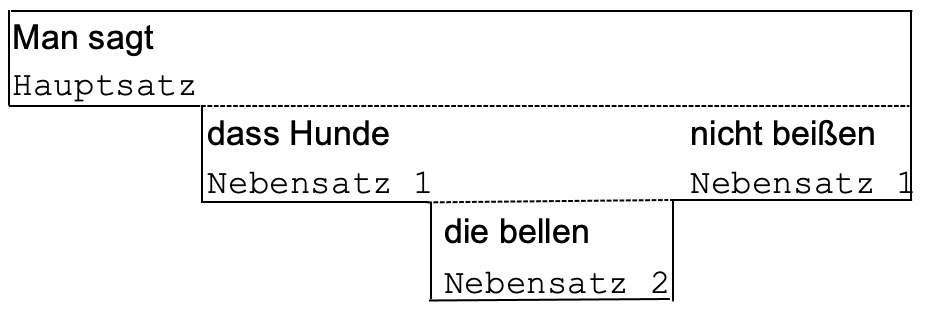
\includegraphics[width=8cm]{figures/Satzbild_Hunde.jpeg}
    %% Abbildung 

	
	\noindent\resizebox{\textwidth}{!}{
	
		\begin{tabular}{  p{3.5cm} p{3.5cm} p{3.5cm} p{3.5cm} }
			
			\hline
			\multicolumn{1}{ | l }{\makecell[l]{Man sagt \\ \small{\textcolor{gray}{Hauptsatz}}}} &&& \multicolumn{1}{ l | }{} \\   \cline{1-1} \sbdashline{2-4}
			
			& \multicolumn{1}{ | l}{\makecell[l]{dass Hunde \\ \small{\textcolor{gray}{Nebensatz 1}}}} & & 
			\multicolumn{1}{ l | }{\makecell[l]{nicht beißen \\ \small{\textcolor{gray}{}}}} \\ \cline{2-2} \sbdashline{3-4} \cline{4-4}
			
			& & \multicolumn{1}{ | l | }{\makecell[l]{die bellen \\ \small{\textcolor{gray}{ Nebensatz 2}}}} & \\ \cline{3-3} 
			
		\end{tabular}
	}
	

	



    \caption{Satzbild zu (\ref{ex:HS_NeSa_NeSa})}
    \label{Abb:Satzbild_Hunde}
\end{figure}

Die jeweilige Ebene wird auch als \textit{Grad} der Einbettung bezeichnet. Daher könnte der Nebensatz der ersten Ebene auch \textit{ersten Grades} genannt werden und der Nebensatz der zweiten Ebene entsprechend \textit{zweiten Grades}.

Nun zurück zu den Satzgliedfunktionen: Der komplexe Nebensatz \textit{dass Hunde, die bellen, nicht beißen} ist das Satzobjekt von \textit{sagt}. Es besteht die wichtigen Satzgliedtests (vgl. Kapitel \ref{chap:Konstituenz}). Der komplexe Nebensatz ist voranstellbar (\ref{ea:dassNeSaTop}), pronominalisierbar (\ref{ex:dassNeSaPrn}), auch durch ein Fragepronomen und somit auch erfragbar (\ref{ex:dassNeSaFrage}).

\ea \label{ea:NeSaSGTests}
\ea \label{ea:dassNeSaTop} [Dass Hunde, die bellen, nicht beißen,] sagt man.
\ex \label{ex:dassNeSaPrn} Man sagt [das].
\ex \label{ex:dassNeSaFrage} [Was] sagt man?
\z 
\z 

Intern besteht das Satzobjekt wieder aus Satzgliedern. Denn es enthält ein Prädikat, nämlich \textit{beißen}. Das Verb ist zweiwertig und verlangt nach einer Ergänzung im Nominativ, dem Subjekt und einer Ergänzung im Akkusativ, dem Objekt. Ein Objekt gibt es nicht. Das Verb wird einwertig gebraucht (vgl. Abschnitt~\ref{subsubsection:TestNOT}). Das Subjekt ist \textit{Hunde, die bellen}. Der Nebensatz ist Teil des Subjektes. Zum Nachweis bilden wir aus dem Nebensatz \textit{dass Hunde, die bellen, nicht beißen} einen Hauptsatz (\ref{ea:HSUmformung}). Der Nebensatz \textit{die bellen} kann nicht alleine im Vorfeld stehen (\ref{ex:RelNeSaTop}), ist nicht durch eine Pro-Form ersetzbar (\ref{ex:RelNeSaPrn}) und nicht alleine erfragbar (\ref{ex:RelNeSaFrage}). 

\ea \label{ea:NeSaAttrTests}
\ea [] {Hunde, die bellen, beißen nicht.}\label{ea:HSUmformung} 
\ex [*] {Die bellen beißen Hunde nicht.}\label{ex:RelNeSaTop}
\ex [*] {Hunde ?? beißen nicht.}\label{ex:RelNeSaPrn}
\ex [*] {Welche beißen Hunde nicht?}\label{ex:RelNeSaFrage}
\z 
\z 

Der Nebensatz \textit{die bellen} ist kein Satzglied, weil er sich auf kein Prädikat bezieht und damit von keinem Prädikat abhängt. Er bezieht sich auf \textit{Hunde}, den Kopf der Subjekt-NP und ist somit Teil des Subjekts \textit{Hunde, die bellen} und damit Attribut. Deshalb ist nur die gemeinsame Voranstellung wie in (\ref{ea:HSUmformung}) möglich.

Attribute werden in der Satzgliedanalyse nicht sichtbar, weil sie keine Satzglieder, sondern Satzgliedteile sind. Aber wenn sie über ein Prädikat wie \textit{bellen} verfügen, bestehen sie intern wieder aus Satzgliedern. Diese werden auf einer tieferen Ebene (in einer weiteren Tabellenspalte) bestimmt. Das Prädikat \textit{bellen} ist einwertig und verlangt nach einer Ergänzung im Nominativ, nach einem Subjekt. Das Subjekt ist das den Relativsatz einleitende Demonstrativpronomen \textit{die}.

Die schrittweise Analyse ausgehend vom Hauptprädikat stellen wir in der Tabelle~\ref{tab:Satzgefüge1} dar. Die im Satzbild (Abbildung~\ref{Abb:Satzbild_Hunde}) dargestellten Ebenen entsprechen bei einer Drehung um 90 Grad nach links den Spalten.

\begin{table}
  \centering
  \begin{tabular}{l|l|l|l}
    %\lsptoprule
     & Hauptsatz & 1. Nebensatzebene & 2. Nebensatzebene \\
    \hline
    \textit{Man} & Subjekt &  & \\
    \cline{2-2} 
    \textit{sagt,} & Prädikat & & \\
    \cline{2-3}
    \textit{dass} & \multirow{6}{*}{Satzobjekt} & -- & \\ \cline{3-3}
    \textit{Hunde,} &  & \multirow{3}{*}{Subjekt} & \\ \cline{4-4}
    \textit{die} & & & Subjekt \\ \cline{4-4}
    \textit{bellen,} & & & Prädikat  \\ \cline{3-4}
    \textit{nicht} & & -- & \\ \cline{3-3}
    \textit{beißen.} & & Prädikat & \\ 
    \hline 
   % \lspbottomrule
  \end{tabular}
  \caption{Satzgefüge mit zwei Einbettungsebenen}
  \label{tab:Satzgefüge1}
\end{table}

Die Nebensatzebenen müssen nicht der Reihenfolge ihres Auftretens entsprechen. Wie in (\ref{ea:HS_mehrereNeSa}) kann ein Hauptsatz auch zwei (und mehr) Nebensätze direkt in sich, also eine Ebene tiefer einbetten. 

\ea \label{ea:HS_mehrereNeSa} Jugendliche, die ihren Freunden eine Nachricht in Facebook schreiben, werden in der Regel nicht lange nachdenken, ob diese oder jene Schreibweise richtig ist.\footnote{Christa Dürscheid (2011): \textit{Zweifeln als Chance? Zweifeln als Problem? Sprachliche Zweifelsfälle im Deutschunterricht.} In: Köpcke, K.-M. \& A. Ziegler (Hrsg.): \textit{Grammatik – Lehren, Lernen, Verstehen. Zugänge zur Grammatik des Gegenwartsdeutschen.} Berlin, Boston: de Gruyter, S. 161.}
\z 

Die Einbettungsebenen stellen wir in der Abbildung~\ref{Abb:Satzbild_Jugendliche} im Satzbild\is{Satzbild} dar.

\begin{figure}
    \centering
   % 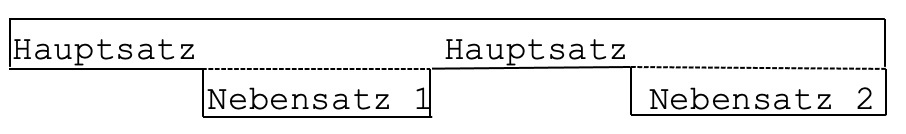
\includegraphics[width=9cm]{figures/Satzbild_Jugendliche.jpeg}
   %% Abbildung 

		\noindent\resizebox{\textwidth}{!}{
		
		\begin{tabular}{p{3cm} p{3cm} p{3cm} p{3cm} | }
			
			\hline
			\multicolumn{1}{ | l }{\makecell[l]{\small{\textcolor{gray}{Hauptsatz}}}} & & 
			\multicolumn{1}{ l }{\makecell[l]{\small{\textcolor{gray}{}}}} &  \\ 
			\cline{1-1} \sbdashline{2-2}  \cline{3-3} \sbdashline{4-4}
			
			
			&  \multicolumn{1}{ | l | }{\makecell[l]{\small{\textcolor{gray}{Nebensatz 1}}}}  & & 
		     	 \multicolumn{1}{ | l | }{\makecell[l]{\small{\textcolor{gray}{Nebensatz 2}}}}   		\\ 
		     	 \cline{2-2}  \cline{4-4}
			
		\end{tabular}
	}
	


	

	



    \caption{Satzbild zu (\ref{ea:HS_mehrereNeSa})}
    \label{Abb:Satzbild_Jugendliche}
\end{figure}

Das Prädikat des Hauptsatzes ist \textit{werden nachdenken}. Es ist zweiwertig und verlangt nach jemandem, der nachdenkt als Subjekt und nach etwas, worüber nachgedacht wird, als Präpositionalobjekt. An dessen Stelle steht der zweite Nebensatz \textit{ob diese oder jene Schreibweise richtig ist} und fungiert damit als Satzobjekt. Das Subjekt ist die komplexe NP im Vorfeld \textit{Jugendliche} zusammen mit dem ersten Nebensatz \textit{die ihren Freunden eine Nachricht in Facebook schreiben}. Beide Nebensätze sind direkt in den Hauptsatz eingebettet. Hierfür steht die gestrichelte Linie auf der Hauptsatzebene. Der erste Nebensatz ist als Attribut Bestandteil des Subjektes. Der zweite Nebensatz ist ein Satzglied, da er als Objekt direkt vom Hauptprädikat abhängt. Die interne Struktur beider Nebensätze wird in einer Spalte, direkt nach der Hauptsatzebene, analysiert, was wir in der Tabelle~\ref{tab:Satzgefüge2} zeigen. 


\begin{table}
  \centering
  \begin{tabular}{l|l|l}
    %\lsptoprule
      &  Hauptsatz & 1. Nebensatzebene \\
    \hline
    \textit{Jugendliche,} & \multirow{9}{*}{Subjekt} &  \\
    \cline{3-3} 
    \textit{die} & & Subjekt \\
    \cline{3-3}
    \textit{ihren} & & \multirow{2}{*}{Dativobjekt} \\ 
    \textit{Freunden} &  & \\ \cline{3-3}
    \textit{eine} & &  \multirow{2}{*}{Akkusativobjekt} \\ 
    \textit{Nachricht} & & \\ \cline{3-3}
    \textit{in} & & \multirow{2}{*}{Adverbial} \\ 
    \textit{Facebook} & & \\ \cline{3-3}
    \textit{schreiben,} & & Prädikat \\ \cline{2-3}
    \textit{werden} & Prädikat &  \\ \cline{2-2}
    \textit{in} & \multirow{3}{*}{Adverbial} & \\ 
    \textit{der} & & \\ 
    \textit{Regel} & & \\ \cline{2-2} 
    \textit{nicht} & \multirow{2}{*}{Adverbial} & \\ 
    \textit{lange} & & \\ \cline{2-2}
    \textit{nachdenken,} & Prädikat & \\ \cline{2-3}
    \textit{ob} & \multirow{7}{*}{Satzobjekt} & -- \\ \cline{3-3}
    \textit{diese} & & \multirow{4}{*}{Subjekt} \\
    \textit{oder} & & \\
    \textit{jene} & & \\ 
    \textit{Schreibweise} & & \\ \cline{3-3}
    \textit{richtig} & & Subjektsprädikativ \\ \cline{3-3}
    \textit{ist.} & & Prädikat \\ 
    \hline 
   %\lspbottomrule
  \end{tabular}
  \caption{Satzgefüge mit einer Einbettungsebene}
  \label{tab:Satzgefüge2}
\end{table}

\vspace{.2cm}

Bevor wir uns mit der Form und Funktion von Nebensätzen in Satzgefügen beschäftigen, fassen wir das Wichtigste zusammen. Wir haben zwischen Satzreihen und Satzgefügen unterschieden. Bei Satzreihen handelt es sich um gleichrangig miteinander verbundene Teilsätze. Im Gegensatz dazu enthält ein Satzgefüge einen nicht-gleichrangig eingebetteten Teilsatz. 


\subsection{Form und Funktion von Nebensätzen}\label{subsection:FormFktNeSa}

Nebensätze\is{Nebensatz!Funktionen} drücken wie Hauptsätze Szenarien aus. Aber sie behaupten diese nicht explizit wie letztere (vgl. Abschnitt~\ref{section:Grundlagen}). In Abschnitt~\ref{section:Satzglieder} haben wir gezeigt, dass Nebensätze die Funktion der wichtigsten Satzglieder sowie die eines Attributs übernehmen können. Sie können in einem Satz als Subjekt (\ref{ea:NeSaSG_Subjekt}), Akkusativobjekt (\ref{ex:NeSaSG_A_Objekt}), Dativobjekt (\ref{ex:NeSaSG_D_Objekt}), Direktivum (\ref{ex:NeSaSG_Dir}), Präpositionalobjekt (\ref{ex:NeSaSG_P_obj}), Prädikativ (\ref{ex:NeSaSG_Prädikativ}) und Adverbial (\ref{ex:NeSaSG_Adv}) fungieren bzw. an dessen Stelle stehen. Innerhalb eines Satzglieds können sie die Rolle des Attributs (\ref{ex:NeSaSG_Attribut}) haben.

\ea \label{ea:NeSaSGFunktion}
\ea \label{ea:NeSaSG_Subjekt} \textit{Dass eine Beteiligung an einem Einsatz im Nahen Osten in Deutschland kontrovers diskutiert wird}, hat niemanden überrascht.\footnote{Nordkurier, 27.09.2006.}
\ex \label{ex:NeSaSG_A_Objekt} Eine Kundin möchte wissen, \textit{ob dieser Pullover beim Waschen einläuft}.\footnote{Rhein-Zeitung, 24.12.2005.}
\ex \label{ex:NeSaSG_D_Objekt} Ich sah zu, \textit{wie das geschmolzene Blei aus dem Teelöffel ins kalte Wasser zischelt} [\ldots{}]\footnote{Herta Müller: \textit{Der König verneigt sich und tötet}. München: Hanser, 2003, S. 58.}
\ex \label{ex:NeSaSG_Dir} Geh, \textit{wohin dein Herz dich trägt}.\footnote{Buchtitel von Susanna Tamaro. Zürich: Diogenes, 1997.}
\ex \label{ex:NeSaSG_P_obj} Ein Passant beschwert sich, \textit{dass er keinen Platz bekommen hat}.\footnote{Mannheimer Morgen, 05.03.2002.}
\ex \label{ex:NeSaSG_Prädikativ} Die Situation ist und bleibt, \textit{wie sie ist}, man verbrennt nur seine Kraft vergeblich.\footnote{Luxemburger Tageblatt, 03.05.2018.}
\ex \label{ex:NeSaSG_Adv} \textit{Wenn es einen Anlass zum Scherzen gibt}, schmunzle ich gern einmal.\footnote{Zitat aus Loriots Film \textit{Papa ante portas}.}
\ex \label{ex:NeSaSG_Attribut} Selbst der Mann, \textit{der niemals lächelte}, hat auf seine diskrete Art Ecken und Kanten [\ldots{}]\footnote{Süddeutsche Zeitung, 25.02.2016.}
\z 
\z 

\textit{Subjunktionalsätze} werden\is{Nebensatz!Subjunktionalsatz}, wie der Name schon sagt, durch eine Subjunktion (vgl. Abschnitt~\ref{subsubsection:Subjunktion}) eingeleitet. \textit{Sub}junktionen verbinden auch Sätze, aber der Satz, den sie einleiten, ist einem anderen Satz oder einem Wort \textit{unter}geordnet. Subjunktionale Nebensätze lassen sich bezüglich ihrer syntaktischen Funktion in zwei große Gruppen einteilen: in solche mit den relativ bedeutungsleeren Subjunktionen \textit{dass} und \textit{ob} und in solche mit den bedeutungsreicheren temporalen, kausalen usw. Subjunktionen wie \textit{nachdem}, \textit{wenn}, usw. 

Die relativ\is{Nebensatz!Subjekt-/Objektfunktion} bedeutungsarmen Subjunktionen \textit{dass} und \textit{ob} leiten Nebensätze ein, die typischerweise als Subjekt- oder Objektsatz verbale Ergänzungen sind. Durch \textit{dass} wird der ausgedrückte Sachverhalt als wahr vorausgesetzt. Durch \textit{ob} bleibt das offen. Beide Subjunktionen sind in dem Nebensatz, den sie einleiten, weder Satzglied noch Attribut. Deshalb setzen wir in der Tabelle einen Strich. Die Analyse stellen wir exemplarisch für (\ref{ex:NeSaSG_A_Objekt}) in Tabelle~\ref{tab:Satzgefüge_mit_ob_Objektsatz} dar.

\begin{table}
  \centering
  \begin{tabular}{l|l|l}
    %\lsptoprule
      & Hauptsatz & 1. Nebensatzebene \\
    \hline
    \textit{Eine} & \multirow{2}{*}{Subjekt} &  \\
    \textit{Kundin} & & \\ \cline{2-2}
    \textit{möchte} & \multirow{2}{*}{Prädikat} & \\ 
    \textit{wissen,} &  & \\ \cline{2-3}
    \textit{ob} & \multirow{6}{*}{Satzobjekt} & -- \\ \cline{3-3} 
    \textit{dieser} &  & \multirow{2}{*}{Subjekt} \\ 
    \textit{Pullover} & & \\ \cline{3-3} 
    \textit{beim} &  & \multirow{2}{*}{Adverbial} \\
    \textit{Waschen} & & \\ \cline{3-3}
    \textit{einläuft.} & & Prädikat  \\ 
    \hline 
   %\lspbottomrule
  \end{tabular}
  \caption{Subjunktionaler Objekt-Nebensatz mit \textit{ob}}
  \label{tab:Satzgefüge_mit_ob_Objektsatz}
\end{table}

In den\is{Nebensatz!Attributfunktion} Abschnitten zum Bau von NPs (vgl. Abschnitt~\ref{section:NP}) und zum Bau von VPs (vgl. Abschnitt~\ref{section:VP}) sowie insbesondere zur Unterscheidung und Überführung zwischen Satzgliedern und Attributen (vgl. Abschnitt~\ref{section:SatzgliederundAttribute}) haben wir auf Nominalisierungen von Verben hingewiesen. Durch diese können auch die Subjunktionen \textit{dass} und \textit{ob} aus dem Verbal- und damit Satzgliedbereich (\ref{ex:NeSaSG_A_Objekt}) in den nominalen Bereich der Attribute vererbt werden (\ref{ea:ob_Attr}).

\ea \label{ea:ob_Attr} Ihr Wissen, \textit{ob dieser Pullover beim Waschen einläuft}, hilft ihr.
\z 

An der internen Struktur des Nebensatzes ändert das nichts, was wir in Tabelle~\ref{tab:Satzgefüge_mit_ob_Attributsatz} darstellen.

\begin{table}
  \centering
  \begin{tabular}{l|l|l}
  %  \lsptoprule
     &  Hauptsatz & 1. Nebensatzebene \\
    \hline
    \textit{Ihr} & \multirow{8}{*}{Subjekt} &  \\
    \textit{Wissen,} & & \\ \cline{3-3}
    \textit{ob} & &  -- \\ \cline{3-3} 
    \textit{dieser} &  & \multirow{2}{*}{Subjekt} \\ 
    \textit{Pullover} & & \\ \cline{3-3} 
    \textit{beim} & & \multirow{2}{*}{Adverbial} \\
    \textit{Waschen} & & \\ \cline{3-3}
    \textit{einläuft,} & & Prädikat  \\ \cline{2-3} 
    \textit{hilft} & Prädikat \\ \cline{2-2}
    \textit{ihr.} & Dativobjekt & \\
    \hline
   %\lspbottomrule
  \end{tabular}
  \caption{Subjunktionaler Attribut-Nebensatz mit \textit{ob}}
  \label{tab:Satzgefüge_mit_ob_Attributsatz}
\end{table}


Subjunktionale Nebensätze\is{Nebensatz!Adverbialfunktion} mit bedeutungsreicheren Subjunktionen wie \textit{als}, \textit{bevor}, \textit{nachdem} \textit{weil}, \textit{obwohl}, \textit{wenn}, \textit{damit}, \textit{indem} usw. leiten typischerweise Adverbialsätze ein. Sie sättigen keine Valenzstellen des Prädikats, sondern spezifizieren das ausgedrückte Szenario (vgl. Abschnitt~\ref{subsection:Adverbial}). Formal besonders sind zweiteilige Subjunktionen wie \textit{als ob}, \textit{anstatt dass}, \textit{ohne dass} oder \textit{so dass}. Bei letzterer wird heute vom Duden die Zusammenschreibung als \textit{sodass} empfohlen.

Unabhängig vom Bedeutungsumfang und von Ein- oder Zweiteiligkeit gibt es zwei wesentliche Gemeinsamkeiten: Subjunktionalsätze sind typischerweise Satzglieder eines übergeordneten Prädikats. Die Subjunktionen selber sind innerhalb des Nebensatzes, den sie einleiten, weder Satzglied noch Attribut. Deshalb setzen wir in der Tabelle auf der entsprechenden Ebene einen Strich. Das haben wir in den Tabellen~\ref{tab:Satzgefüge1}, \ref{tab:Satzgefüge2} und \ref{tab:Satzgefüge3} gesehen.

Eine formale\is{Nebensatz!verkappter} Besonderheit stellen \textit{uneingeleitete Nebensätze} (\ref{ea:verkappteNeSa}) dar. Diese bilden wir ohne Subjunktion. Folglich steht auch der finite Prädikatsteil nicht in der rechten, sondern in der linken Satzklammer. 

\ea \label{ea:verkappteNeSa}
\ea \label{ea:verkappterObjektsatz} Paul sagt, \textit{er komme später}.
\ex \label{ex:verkappterKondNeSa} \textit{Regnet es stark}, bleiben wir zu Hause.
\ex \label{ex:verkappterMODalsNeSa} Er tut so, \textit{als sehe er mich nicht}.
\z 
\z 

In (\ref{ea:verkappterObjektsatz}) könnte es heißen \textit{dass er später komme}, in (\ref{ex:verkappterKondNeSa}) \textit{wenn es stark regnet} und in (\ref{ex:verkappterMODalsNeSa}) \textit{als ob er mich nicht sehe}.    

Obwohl das finite Verb in den kursiv gesetzten Teilsätzen in (\ref{ea:verkappteNeSa}) nicht am Ende steht, handelt es sich um Nebensätze. Denn sie hängen vom Bezugsprädikat bzw. von dem anderen Teilsatz ab. Mit \citet[70]{Welke2007} nehmen wir für solche Nebensätze mit Verbzweit- und Verberststellung die Bezeichnung \textit{verkappter Nebensatz} wieder auf. 

In (\ref{ea:verkappterObjektsatz}) handelt es sich um das Objekt zu \textit{sagt}. Nach \citet[119]{Bausewein1990} stellt diese Realisierungsform die häufigere Variante dar.\footnote{Im Gegensatz zu \citet[119]{Bausewein1990} bezeichnen \citet[167]{OehlSeiler2013} solche uneingeleiteten Nebensätze als \gqq{Ausnahme}. Nach verneinten Verben des Sagens und Denkens sind solche uneingeleiteten Nebensätze weniger gebräuchlich: \textit{Er behauptete nicht,} ?\textit{er sei unschuldig}. Bei Interesse empfehlen wir auch \citet[121]{Reis1997}, die von \gqq{syntaktisch relativ unintegrierten Nebensätze[n]} schreibt.} In (\ref{ex:verkappterKondNeSa}) drückt der verkappte Nebensatz mit Verberststellung ein bedingendes Szenario aus und fungiert als konditionales Adverbial. In (\ref{ex:verkappterMODalsNeSa}) geht es um die Beschreibung der Art und Weise (\textit{als sehe er mich nicht}). Es handelt sich um ein modales Adverbial. Auf das \textit{so} gehen wir in Abschnitt~\ref{subsection:Korrelat} unter dem Stichwort \textit{Korrelat} ein.  

Nicht-subjunktionale Nebensatzeinleiter haben innerhalb des Nebensatzes, den sie einleiten, eine Satzgliedfunktion. Das ist\is{indirekter Fragesatz} der Fall bei sogenannten \textit{indirekten Frage-Nebensätzen} mit Fragewörtern wie \textit{wer}, \textit{welcher}, \textit{wo}, \textit{warum} oder durch \textit{w}-Pro-Präpositionsgruppen (vgl. Abschnitt~\ref{section:Pronominalisierung}) wie \textit{worauf}, \textit{womit}, \textit{wofür}, usw. aus. 

\ea \label{ea:Frage-NeSa}
\ea \label{ea:wissen_warum} Ich weiß doch, \textit{warum du uns das erzählst}. \footnote{Sven Regener: \textit{Herr Lehmann}. Frankfurt am Main: Eichborn, 2001, S. 137.}
\ex \label{ex:fragen_woran} Ich frage ihn, \textit{woran er leidet}.\footnote{Die Zeit, 16.03.2000}
\z 
\z 

Als Ganzes fungieren auch indirekte Frage-Nebensätze als Satzobjekt bei Verben des Fragens, (Nicht)-Wissens und Wahrnehmens. Aber innerhalb des Nebensatzes sind die Fragewörter Satzglieder. In (\ref{ea:wissen_warum}) ist \textit{warum} ein Kausaladverbial, da es für die Angabe eines Grundes für den Sachverhalt \textit{du erzählst uns das} steht. Die Pro-Form \textit{woran} steht in (\ref{ex:fragen_woran}) für das Präpositionalobjekt von \textit{leidet}. Die Analyse von (\ref{ex:fragen_woran}) stellen wir in der Tabelle~\ref{tab:FrageNeSa} dar.

\begin{table}
  \centering
  \begin{tabular}{l|l|l}
    %\lsptoprule
      & Hauptsatz & 1. Nebensatzebene \\
    \hline
    \textit{Ich} & Subjekt &  \\ \cline{2-2}
    \textit{frage} & Prädikat & \\ \cline{2-2}
    \textit{ihn,} & Akkusativobjekt & \\ \cline{2-3}
    \textit{woran} & \multirow{3}{*}{Satzobjekt} & Präpositionalobjekt \\ \cline{3-3}  
    \textit{er} & & Subjekt  \\ \cline{3-3} 
    \textit{leidet.} & & Prädikat \\ 
    \hline 
  % \lspbottomrule
  \end{tabular}
  \caption{Nebensatzeinleitende Pronomen mit Satzgliedwert}
  \label{tab:FrageNeSa}
\end{table}

Typische Attribut-Nebensätze\is{Relativsatz} sind\is{Nebensatz!Attributfunktion} \textit{Relativsätze}. Sie werden durch Pronomen wie \textit{der}, \textit{den}, \textit{dem} oder \textit{welcher}, \textit{welchem}, usw. eingeleitet (\ref{ea:DP_Rel}). 

\ea \label{ea:DP_Rel} Das ist der Mann, \textit{den}/\textit{welchen} Anna gestern getroffen hat.
\z 

Die im Relativsatz gebrauchten Pronomen kongruieren im Genus und Numerus mit dem Bezugswort. Der Kasus richtet sich nach ihrer syntaktischen Funktion im Relativsatz. Um die Formen der Pronomen geht es im Abschnitt~\ref{subsection:Pronomen_Flexion}.

Ebenso können Relativsätze durch Adverbien wie \textit{wo}, \textit{wohin} und \textit{woher} eingeleitet werden (\ref{ea:Adv_Rel}). Ihre Form ist unveränderlich.  

\ea \label{ea:Adv_Rel} Paul wohnt, \textit{wo} Fuchs und Hase sich gute Nacht sagen.
\z 

Mit Relativsätzen\is{Relativsatz!restriktiv} werden Merkmale des von einer NP Bezeichneten ausbuchstabiert. Die Merkmalsübertragung geschieht auf zwei grundlegende Arten. Durch \textit{restriktive} Relativsätze wird die Menge des potenziell Bezeichneten eingeschränkt (restringiert). So geht es in (\ref{ea:restriktivREL}) nicht um alle möglichen Menschen, sondern nur um die Untermenge der über 65-Jährigen. 

\ea \label{ea:restriktiv_appositiv}
\ea \label{ea:restriktivREL}  Der Trend betrifft jedoch hauptsächlich Menschen, \textit{die das 65. Lebensjahr überschritten haben}.\footnote{Süddeutsche Zeitung, 25.08.2015.}
\ex \label{ex:appositivREL} Die Figuren aus dem beliebten Kinderbuch, \textit{das jetzt verfilmt wurde}, gibt es beim Kaufhof.\footnote{Mannheimer Morgen, 03.12.2004.}
\z 
\z 

In (\ref{ex:appositivREL}) schränkt der\is{Relativsatz!appositiv} Relativsatz nicht die Referenz der NP ein. Er gibt eine zusätzliche Information über das von der NP Bezeichnete, weshalb man von \textit{appositiv}en Relativsätzen spricht. Diese Lesart kann durch das Hinzufügen von \textit{übrigens} getestet oder ausgelöst werden. 


In der Satzgliedanalyse wird dieser Unterschied nicht erfasst. Exemplarisch analysieren wir den Satz (\ref{ex:appositivREL}) in der Tabelle~\ref{tab:Relativsatz}.

\begin{table}
  \centering
  \begin{tabular}{l|l|l}
   % \lsptoprule
        & Hauptsatz & 1. Nebensatzebene \\
    \hline
    \textit{Die} & \multirow{9}{*}{Akkusativobjekt} &  \\ 
    \textit{Figuren} & & \\
    \textit{aus} & & \\
    \textit{dem} & & \\ 
    \textit{beliebten} & & \\ 
    \textit{Kinderbuch,} & & \\ \cline{3-3}
    \textit{das} & & Subjekt \\ \cline{3-3}
    \textit{jetzt} & & Adverbial \\ \cline{3-3}
    \textit{verfilmt} & & \multirow{2}{*}{Prädikat} \\
    \textit{wurde,} & & \\ \cline{2-3} 
    \textit{gibt} & Prädikat & \\ \cline{2-2}
    \textit{es} & Subjekt & \\ \cline{2-2}
    \textit{im} & \multirow{2}{*}{Adverbial} &  \\   
    \textit{Kaufhof.} & & \\  
    \hline 
  % \lspbottomrule
  \end{tabular}
  \caption{Relativsatz}
  \label{tab:Relativsatz}
\end{table}

Von den beschriebenen typischen Zusammenhängen zwischen Form und syntaktischer Funktion gibt es Übergänge. Diese stellen wir in dem folgenden Exkurs~\ref{Exkurs: Übergänge Nebensatzfunktionen} dar. Zuvor fassen wir das Wichtigste zusammen. 

\vspace{.2cm}

Wir haben subjunktionale von uneingeleiteten (verkappten) Nebensätzen unterschieden. 

\begin{itemize}
    \item Subjunktionale Nebensätze mit den bedeutungsarmen Subjunktionen \textit{dass} und \textit{ob} fungieren typischerweise als Subjekte oder Objekte.

    \item Subjunktionale Nebensätze mit den bedeutungsreicheren Subjunktionen wie \textit{bevor}, \textit{indem} oder \textit{weil} fungieren typischerweise als Adverbiale.

    \item Uneingeleitete Nebensätze fungieren typischerweise als Objekte zu Prädikaten des Sagens und Denkens.

\end{itemize}

Subjunktionen kommt innerhalb des Nebensatzes, den sie einleiten, kein Satzgliedstatus zu. Bei Nebensätzen, die durch Demonstrativpronomen wie \textit{der}, \textit{die}, \textit{das}, durch w-Pronomen wie \textit{wer} und \textit{was} sowie durch Frageadverbien wie \textit{wo} und \textit{wohin} eingeleitet sind, ist das nicht der Fall. Diesen Nebensatzeinleitern kommt innerhalb des Nebensatzes eine Satzgliedfunktion zu.

\begin{itemize}
    \item Indirekte Frage-Nebensätze mit \textit{wer}, \textit{was}, \textit{wo} usw. fungieren typischerweise als Objekte zu Prädikaten des Fragens, des (Nicht-)Wissens und des Wahrnehmens. Innerhalb des Nebensatzes fungiert der \textit{w}-Ausdruck als Satzglied.

    \item Relativsätze sind typischerweise Attribute zu einem Substantiv. Die Relativsatzeinleiter fungieren innerhalb des Relativsatzes als Satzglieder.
    
\end{itemize}


\begin{Exkurs}{Funktionsübergänge bei Nebensätzen}\label{Exkurs: Übergänge Nebensatzfunktionen}
    
Innerhalb bestimmter Kontexte können bestehende Nebensatzformen neue Funktionen übernehmen. Bei Nebensätzen mit \textit{dass} und \textit{ob} haben wir auf solche Funktionsübergänge schon hingewiesen. Wenn wir statt der verbalen Prädikate \textit{wissen} oder \textit{fragen} die Substantive (\textit{das}) \textit{Wissen} und (\textit{die}) \textit{Frage} gebrauchen, so werden die ursprünglichen Objektsätze zu Attributsätzen: \textit{das Wissen, dass sich die Erde erwärmt} und \textit{die Frage, ob wir das gestoppt bekommen}. 

Auch auf der Ebene der subjunktionalen Adverbialsätze kann es zu folgenden Funktionsübergängen kommen. Wir können als Adverbial angelegte konditionale \textit{wenn}-Nebensätze (\ref{ea:wenn_Adv}) dann als Satzobjekte verstehen, wenn das übergeordnete Prädikat eine entsprechende Leerstelle hat, die nicht anderweitig besetzt ist (\ref{ex:wenn_Obj}).

\ea \label{ea:wenn_Adv_Obj}
\ea [] {Anna mag Paul (dann) nicht, \textit{wenn er betrunken ist}.}\label{ea:wenn_Adv}
\ex [] {Anna mag (es) nicht, \textit{wenn Paul betrunken ist}.}\label{ex:wenn_Obj}
\ex [\#] {Anna mag es dann nicht, \textit{wenn Paul betrunken ist}.}\label{ex:wenn_Obj_*dann} 
\z 
\z 

Die originäre Funktion des Nebensatzes ist die des Adverbials (\ref{ea:wenn_Adv}). Es drückt eine Bedingung für das Paul-Nicht-Mögen-Szenario aus. Die adverbiale Funktion des Nebensatzes kann im Hauptsatz durch \textit{dann} angezeigt werden. Da \textit{mögen} zweiwertig ist, verstehen wir in (\ref{ex:wenn_Obj}) den Nebensatz als das, was nicht gemocht wird und somit als Objekt. Ohne \textit{es} (vgl. Abschnitt~\ref{subsection:Korrelat}) muss der \textit{wenn}-Satz als Objekt verstanden werden. Das Adverbial \gq{rutscht} in die vom Prädikat angelegte Objektfunktion. \citet[447]{Pittner2013} bezeichnet diese \textit{wenn}-Sätze als \gqq{Zwittererscheinung}. \citet[358]{Eisenberg2020_Satz} bezeichnet diesen \textit{wenn}-Gebrauch als den \gqq{einzige[n] Ausreißer} aus der Adverbialfunktion. Soll die Objektlesart beibehalten werden, so darf das adverbiale \textit{dann} nicht im Hauptsatz stehen (\ref{ex:wenn_Obj_*dann}). Oder aber wir verstehen \textit{es} als Pronomen, das \zB auf das Abendessen verweist. Dann verstehen wir den Nebensatz wieder als das, was er eigentlich ist, nämlich als Adverbial. Die Objektlesart in (\ref{ex:wenn_Obj}) wird durch die offene Valenzstelle des Verbs über die Adverbialfunktion gelegt. Dies führt insbesondere bei Verben \textit{sich freuen} oder \textit{sich ärgern} zu Doppeldeutigkeiten. Denn diese Verben können sowohl ein- als auch zweiwertig gebraucht werden. Nur bei zweiwertiger Lesart (\textit{sich über etw. ärgern}/\textit{freuen}) wird die adverbiale von der Objektfunktion überblendet (\ref{ea:sich_freuen_wenn}).

\ea \label{ea:sich_freuen_wenn} Anna freut sich, \textit{wenn Paul sie besucht}.
\z 

Die primäre adverbiale Lesart ist die, dass Pauls Besuch die Bedingung für Annas Freude ist. Aber durch die mögliche Zweiwertigkeit von \textit{sich} (\textit{über etw.}) \textit{freuen} kann der Nebensatz als das verstanden werden, \textit{worüber} sich Anna freut.

Auch bei Relativsätzen, die typischerweise Attribute sind, gibt es Umstrukturierungen. Manche Relativsätze bezeichnet man als \textit{freie Relativsätze}\is{Relativsatz!freier}. Von \textit{frei} wird gesprochen, weil sie kein Bezugswort im übergeordneten Satz, von dem sie abhängen, haben. Sie werden wie in (\ref{ea:uneingeleiteterREL}) durch \textit{w}-Pronomen und Adverbien eingeleitet.

\ea \label{ea:uneingeleiteterREL}
\ea \label{ea:uneingeleiteterRELwas} Früher musste man essen, \textit{was auf den Tisch kam}.
\ex \label{ex:uneingeleiteterRELwer} Er grüßt, \textit{wen er kennt}.
\ex \label{ex:uneingeleiteterRELwonach} Sie fand, \textit{wonach sie suchte}.
\ex \label{ex:uneingeleiteterRELwo} Er lebt, \textit{wo Fuchs und Hase sich gute Nacht sagen}.
\ex \label{ex:uneingeleiteterRELwohin} Er geht, \textit{wohin auch sie geht}.
\z 
\z 

Diese Relativsätze\is{Satzglied!versus Attribut} verweisen wie NPs mit einem eingebetteten attributiven Relativsatz auf Dinge, Personen oder Orte. \citet[2270--2271]{ZifHoffStr1997} bezeichnen sie deshalb als \gqq{gegenstandsfundiert}. Als Nebensätze sind sie das nicht \gq{per se}, da Sätze per Definition durch ein Prädikat und von ihm abhängige Satzglieder Szenarien ausdrücken. Sie \gq{rutschen} in eine Funktion gegenüber dem übergeordneten Prädikat. In (\ref{ea:uneingeleiteterRELwas}) geht es um Speisen, die gegessen werden, also um Objektfunktion, weshalb es sich um ein Satzobjekt handelt. Auch der Relativsatz in (\ref{ex:uneingeleiteterRELwer}) sättigt die Objektstelle von \textit{grüßt}. Das Gleiche ist in (\ref{ex:uneingeleiteterRELwonach}) der Fall. Der Relativsatz sättigt die Objektstelle von \textit{fand}. In (\ref{ex:uneingeleiteterRELwo}) wird der Relativsatz als Ort des Lebens, also in adverbialer Funktion verstanden. Der Nebensatz in (\ref{ex:uneingeleiteterRELwohin}) übernimmt die Richtungsergänzung des übergeordneten Prädikats \textit{geht} und fungiert damit als Direktivum. Die Analyse wird exemplarisch anhand von (\ref{ex:uneingeleiteterRELwonach}) in Tabelle~\ref{tab:freierRelativsatz} gezeigt.

\begin{table}
  \centering
  \begin{tabular}{l|l|l}
    %\lsptoprule
     &  Hauptsatz  & 1. Nebensatzebene \\
    \hline
    \textit{Sie} & Subjekt &  \\ \cline{2-2}
    \textit{fand,} & Prädikat & \\ \cline{2-3}
    \textit{wonach} & \multirow{3}{*}{Satzobjekt} & Präpositionalobjekt \\ \cline{3-3}
    \textit{sie} &  & Subjekt  \\ \cline{3-3}   
    \textit{suchte.} & & Prädikat \\ 
    \hline 
  % \lspbottomrule
  \end{tabular}
  \caption{Freier Relativsatz}
  \label{tab:freierRelativsatz}
\end{table}

Dass diese Relativsätze \gq{eigentlich} Attribute auf nominaler und nicht Satzglieder auf verbaler Ebene sind, zeigt die mögliche Umformung. Durch ein Pronomen im Hauptsatz werden sie wieder bei gleicher Bedeutung zu Attributen (\ref{ea:uneingeleiteterRELKOR}).

\ea \label{ea:uneingeleiteterRELKOR}
\ea \label{ea:uneingeleiteterRELwasKOR} Früher musste man \textit{das} essen, \textit{was auf den Tisch kam}.
\ex \label{ex:uneingeleiteterRELwerKOR} Er grüßt \textit{den}, \textit{den er kennt}.
\ex \label{ex:uneingeleiteterRELwonachKOR} Sie fand \textit{das}, \textit{wonach sie suchte}.
\ex \label{ex:uneingeleiteterRELwoKOR} Er lebt \textit{dort}, \textit{wo Fuchs und Hase sich gute Nacht sagen}.
\ex \label{ex:uneingeleiteterRELwohinKOR} Er geht \textit{dorthin}, \textit{wohin auch sie geht}.
\z 
\z 

Die Analyse zeigen wir exemplarisch anhand von (\ref{ex:uneingeleiteterRELwonachKOR}) in Tabelle~\ref{tab:Relativsatz_mit_pronominalem_Bezugswort}. Der Relativsatz erfüllt jetzt seine eigentliche Funktion als Attribut innerhalb des Akkusativobjekts \textit{das, wonach sie suchte}. Seine interne Struktur bleibt wie in \ref{tab:freierRelativsatz} unverändert.

\begin{table}
  \centering
  \begin{tabular}{l|l|l}
    %\lsptoprule
     & Hauptsatz &  1. Nebensatzebene \\
    \hline
    \textit{Sie} & Subjekt &  \\ \cline{2-2}
    \textit{fand} & Prädikat & \\ \cline{2-2}
    \textit{das,} & \multirow{4}{*}{Akkusativobjekt} & \\ \cline{3-3}
    \textit{wonach} & & Präpositionalobjekt \\ \cline{3-3}
    \textit{sie} &  & Subjekt  \\ \cline{3-3}   
    \textit{suchte.} & & Prädikat \\  
    \hline
 %  \lspbottomrule
  \end{tabular}
  \caption{Relativsatz mit pronominalem Bezugswort}
  \label{tab:Relativsatz_mit_pronominalem_Bezugswort}
\end{table}

Der \gq{Ausflug} freier Relativsätze in die Domäne der Satzglieder wird formal nur beim Vergleich von (\ref{ex:uneingeleiteterRELwer}) \textit{grüßt, wen er kennt} mit (\ref{ex:uneingeleiteterRELwerKOR}) \textit{grüßt den, den er kennt} ersichtlich. 

Andere Indizien dafür, dass es sich bei Satzgliedern in Form von Relativsätzen um eine grammatische Nische handelt, bietet der Vergleich von valenziell angelegten indirekten Frage-Nebensätzen mit freien Relativsätzen. \citet[346]{Eisenberg2020_Satz} und \citet[446--446]{Pittner2013} weisen auf eine Doppeldeutigkeit hin, die durch Prädikate wie \textit{verrät} in (\ref{ea:verratenFragesatz_frRel}) möglich ist. Wir können \textit{verraten} als ein Mitteilungsverb verstehen, mit dem zu verratenden Ereignis als Objektsatz (\textit{verraten}, \textit{dass}) oder im Sinne von \gq{denunzieren} (\textit{jemanden verraten)}, das nach einem Akkusativobjekt verlangt.

\ea \label{ea:verratenFragesatz_frRel} Sie verrät nicht, \textit{wen sie liebt}.\footnote{Das Beispiel stammt aus \citet[447]{Pittner2013}.}
\z 

Entweder geht es um einen indirekten Frage-Nebensatz. Dann bezieht sich das Szenario \textit{wen sie liebt} als Satzobjekt auf das Prädikat \textit{verrät}. Eine Paraphrase wäre: \gq{sie sagt nicht, wen sie liebt}. In diesem Fall kann kein Pronomen als Bezugswort hinzugefügt werden, weil es kein freier Relativsatz ist (\ref{ea:Frage_ohne_Bezug}). Oder aber wir interpretieren den Nebensatz als freien Relativsatz, also wie eine Entität. Die Paraphrase wäre: \gq{Sie verrät nicht die geliebte Person}. In diesem Fall kann ein Pronomen als Bezugswort eingefügt werden und aus dem freien Relativsatz wird wieder ein Attributsatz wie in (\ref{ex:frRel_mit_Bezug}). 

\ea \label{ea:TestFrage_Relativ}
\ea [*] {Sie verrät (\gq{sagt}) nicht den, den sie liebt.}\label{ea:Frage_ohne_Bezug} 
\ex [] {Sie verrät nicht den, den sie liebt.}\label{ex:frRel_mit_Bezug}
\z 
\z 

Dass Relativsätze\is{Nebensatz!weiterführender} in anderer als der Attributfunktion Nischen sind, zeigt sich auch an sogenannten \textit{weiterführenden Nebensätzen}. Diese sehen aus wie freie Relativsätze mit \textit{w}-Wörtern. Aber sie können nicht wie eine NP als Satzglied auf das übergeordnete Prädikat bezogen werden, weil dieses wie \textit{schneien} in (\ref{ea:regnen_worüber}) gar nicht über eine entsprechende Leerstelle verfügt.

\ea \label{ea:regnen_worüber} Es schneite endlich, worüber sich die Kinder freuten.
\z 

In diesem Fall ist der Relativsatz funktional nicht in den übergeordneten Satz eingebettet. Er bezieht sich auf das gesamte Schneien-Szenario, in dem er keinen Satzgliedwert hat. Die Analyse zeigen wir in Tabelle~\ref{tab:weiterführenderNeSa}.

\begin{table}
  \centering
  \begin{tabular}{l|l|l}
    %\lsptoprule
     &  Hauptsatz  &  1. Nebensatzebene \\
    \hline
    \textit{Es} & Subjekt &  \\ \cline{2-2}
    \textit{schneite} & Prädikat & \\ \cline{2-2}
    \textit{endlich,} & Kommentaradverbial \\ \cline{2-3}
    \textit{worüber} & & Präpositionalobjekt \\ \cline{3-3}
    \textit{sich} &  & Prädikat  \\ \cline{3-3}   
    \textit{die} & & \multirow{2}{*}{Subjekt} \\ 
    \textit{Kinder} & & \\ \cline{3-3} 
    \textit{freuten.} & & Prädikat \\
  % \lspbottomrule
  \hline 
  \end{tabular}
  \caption{Weiterführender Nebensatz}
  \label{tab:weiterführenderNeSa}
\end{table}

Wirklich \textit{frei} sind Relativsätze, wie andere Nebensätze, nie. Denn sie sind strukturell als Attribute eines Bezugsworts angelegt. Gibt es dieses Bezugswort nicht, bleiben zwei Möglichkeiten. Entweder passt der Relativsatz wie eine NP, deren Teil er gewöhnlich ist, in die Leerstelle eines Prädikats als Satzglied (sogenannter \textit{freier Relativsatz}). Dann ist er nicht frei, sondern in Satzgliedfunktion gebunden. Oder er fungiert als sogenannter \textit{weiterführender} Nebensatz zu dem vom übergeordneten Prädikat und dessen Satzgliedern ausgedrückten Szenario. In diesem Fall bezieht er sich analog zum Nomen auf ein ganzes Szenario, als wäre es ein Gegenstand. Dafür spricht die Doppeldeutigkeit in (\ref{ea:lesen_was}). 

\ea \label{ea:lesen_was} Er liest, \textit{was ihn interessiert}.
\z 

Entweder wird \textit{was ihn interessiert} gegenstandsfundiert als Objekt des zweiwertigen Prädikats \textit{liest} verstanden im Sinne von \gq{er liest das, was ihn interessiert}. Oder der Nebensatz bezieht sich auf das einwertige Lesen-Szenario im Sinne von: \gq{Er liest. Das interessiert ihn}. In diesem Fall hat der Nebensatz im übergeordneten Satz keine Funktion.

Beide Lesarten stellen wir nur bezüglich des Satzganzen in Tabelle~\ref{tab:weiterführenderNeSa_frRel} dar. Die interne Struktur des Nebensatzes bleibt unverändert: \textit{was} ist Subjekt, \textit{ihn} Akkusativobjekt und \textit{interessiert} Prädikat.

\begin{table}
  \centering
  \begin{tabular}{l|l|l}
   % \lsptoprule
      & Prädikatsbezug  & Satzbezug\\
    \hline
    \textit{Er} & \multicolumn{2}{c}{Subjekt}\\ \cline{2-3}
    \textit{liest,} & \multicolumn{2}{c}{Prädikat} \\ \cline{2-3}
    \textit{was} & \multirow{3}{*}{Satzobjekt} & \\ 
    \textit{ihn} & & \\ 
    \textit{interessiert.} &  & \\ 
    \hline 
  % \lspbottomrule
  \end{tabular}
  \caption{Freier Relativsatz oder weiterführender Nebensatz}
  \label{tab:weiterführenderNeSa_frRel}
\end{table}

\end{Exkurs}



\subsection{Korrelat oder Kern-Attribut-Beziehung}\label{subsection:Korrelat}

Als \textit{Korrelate} bezeichnet\is{Korrelat} man Wörter in einem übergeordneten Satz, die sich auf einen abhängigen Nebensatz beziehen. Sie korrelieren mit diesem. Der Prototyp ist\is{es@\textit{es}!Korrelat} \textit{es} im Mittelfeld des übergeordneten Satzes. Dieses \textit{es} verweist auf einen im Nachfeld stehenden Nebensatz in Objekt- (\ref{ea:es_Objekt}) oder Subjektfunktion (\ref{ex:es_Subjekt}). In beiden Sätzen könnte \textit{es} auch weggelassen werden, was durch Klammern dargestellt wird. Bei wenigen Verben ist es obligatorisch.\footnote{\citet[99]{HelbigBuscha} geben eine Übersicht über Verben mit obligatorischem, fakultativem und unmöglichem Korrelat.}

\ea \label{ea:es_Korrelat}
\ea \label{ea:es_Objekt} Sie bedauert (\textit{es}), \textit{dass die Nachtzüge verschwinden}.\footnote{Süddeutsche Zeitung, 10.12.2016.}
\ex \label{ex:es_Subjekt} Wen interessiert (\textit{es}), \textit{dass immer mehr Menschen an den Folgen von Industrie- und Verkehrsverschmutzungen sterben}?\footnote{Rhein-Zeitung, 22.03.2018.} 
\z 
\z 


\begin{Definition}{Korrelat}

\noindent 
Korrelate verweisen innerhalb eines Satzes aus einem übergeordneten Teilsatz auf einen vorangehenden oder folgenden untergeordneten Teilsatz. 
\end{Definition}



Anstelle der Satzgefüge mit oder ohne Korrelat in (\ref{ea:es_Korrelat}) sind auch zwei Hauptsätze denkbar (\ref{ea:HS_HS_es_Prn}). Das Pronomen \textit{es} sättigt dann im jeweils zweiten Satz die vom Verb geforderte Objekt- (\ref{ea:es_Objekt_Prn}) bzw. die Subjektstelle (\ref{ex:es_Subjekt_Prn}) und verweist auf die im jeweils ersten Hauptsatz ausgedrückte Situation.

\ea \label{ea:HS_HS_es_Prn}
\ea \label{ea:es_Objekt_Prn} Die Nachtzüge verschwinden. Sie bedauert es.
\ex \label{ex:es_Subjekt_Prn} Immer mehr Menschen sterben an den Folgen von Industrie- und Verkehrsverschmutzungen. Wen interessiert es? 
\z 
\z 

Möglich wäre es auch, den jeweils ersten Hauptsatz als Nebensatz direkt, das heißt ohne Korrelat, in den zweiten Hauptsatz zu integrieren. In diesem Fall handelt es sich um ein Satzobjekt bzw. ein Subjekt. Die Nebensätze sind dann voranstellbar (\ref{ea:es_Korrelat_NeSa_Top}).

\ea \label{ea:es_Korrelat_NeSa_Top}
\ea \label{ea:es_Objekt_NeSa_Top} \textit{Dass die Nachtzüge verschwinden}, bedauert sie. 
\ex \label{ex:es_Subjekt_NeSa_Top} \textit{Dass immer mehr Menschen an den Folgen von Industrie- und Verkehrsverschmutzungen sterben}, interessiert wen? 
\z 
\z 

Bei dem Ausdrucksmuster mit Korrelat und Nebensatz (\ref{ea:es_Korrelat}) stellt sich die Frage nach ihrem jeweiligen syntaktischen Status. Denn eine Objekt- oder Subjektstelle kann nur einmal besetzt werden (vgl. Abschnitt~\ref{subsubsection:TestINSP}). 

Im Rahmen der Satzgliedtheorie bietet sich primär die folgende Analyse an: Das Pronomen \textit{es} ist in (\ref{ea:es_Objekt}) der Kern des Akkusativobjekts und in (\ref{ex:es_Subjekt}) der Kern des Subjekts. Die Nebensätze sind dann Attribute innerhalb des Akkusativobjekts bzw. innerhalb des Subjekts. Strukturen dieser Art haben wir bereits bei den sogenannten freien Relativsätzen kennengelernt, wenn sie an ein Pronomen im übergeordneten Satz gebunden werden (\textit{das finden, wonach gesucht wird}).


Attributsätze können eigentlich nur zusammen mit ihrem pronominalen Bezugswort vorangestellt werden (\ref{ea:Prn_Attr_Top}). Aber \textit{es} kann gerade das nicht (\ref{ex:*es_Attr_Top}).

\ea \label{ea:NeSa_Kor_Top}
\ea [] {\textit{Ihn, der alles verloren hat,} bedauert sie.}\label{ea:Prn_Attr_Top}
\ex [*] {\textit{Es, dass die Nachtzüge verschwinden,} bedauert sie.}\label{ex:*es_Attr_Top}
\z 
\z 


Die Stellungseigenschaften und die Tatsache, dass gerade der Nebensatz die inhaltliche Füllung des Satzglieds gewährleistet, sprechen gegen die Bestimmung von \textit{es} als Kern des Subjekts oder Objekts mit integriertem Attributsatz. Das Korrelat\is{es@\textit{es}!Korrelat} \textit{es} zeigt nicht auf eine Entität oder auf ein Geschehen, welche durch den Nebensatz eingegrenzt oder näher bestimmt würde. \textit{Es} ist nicht betonbar und nicht fokussierbar (*\textit{ihn interessiert nur es, dass}). 

Das Korrelat \textit{es} kündigt im Mittelfeld an, dass später noch ein Objekt oder Subjekt in Form eines Nebensatzes folgt.\footnote{\citet[907]{Oppenrieder2006} schreibt valenzgebundenen satzförmigen Ausdrücken eine \gqq{potentielle Ankündbarkeit} durch ein Korrelat zu. In diesem Sinne bezeichnet \citet[589]{Agel2017} die Funktion von \textit{es} als \gqq{kategoriale Anzeige}.} Dabei leistet das Pronomen, was der Nebensatz nicht kann. Es erfüllt als Nominativ- oder Akkusativpronomen die formale Valenzforderung des Verbs, welche inhaltlich später durch den Nebensatz gefüllt wird. In diesem Sinne beschreibt \citet[167]{Breindl1989} die Funktion als \gqq{vorausweisende Dekodierungshilfe}.\footnote{Für weitere textuelle Faktoren verweisen wir auf \citet[453--454]{Pittner2013}.} 

\citet[353]{Eisenberg2020_Satz} bestimmt das Korrelat als formalen, da kasustragenden Kopf und den Nebensatz als semantischen Kern derjenigen Konstituente, die als Objekt oder Subjekt fungiert.\footnote{Letztlich geht es um eine analoge Analyse zum Artikel als grammatischem und dem Nomen als semantischem Zentrum einer NP. Eine knappe Übersicht und Kritik bietet \citet[451]{Pittner2013}.} Wir stellen die Analyse in der Tabelle~\ref{tab:ObjKorr_NeSaObj} anhand von (\ref{ea:es_Objekt}) dar. 

\begin{table}
  \centering
  \begin{tabular}{l|l|l}
    %\lsptoprule
      &  Hauptsatz   &  1. Nebensatzebene \\
    \hline
    \textit{Sie} & Subjekt  & \\ \cline{2-2}
    \textit{bedauert} & Prädikat  & \\ \cline{2-2} 
    \textit{es,} & Akk-Obj-Korrelat & \\ \cline{2-3} 
    \textit{dass} & \multirow{4}{*}{Satzobjekt} & -- \\ \cline{3-3}
    \textit{die} & & \multirow{2}{*}{Subjekt} \\ 
    \textit{Nachtzüge} & & \\ \cline{3-3}
    \textit{verschwinden.} & & Prädikat \\
    \hline 
  % \lspbottomrule
  \end{tabular}
  \caption{Objekt-Korrelat und Satzobjekt}
  \label{tab:ObjKorr_NeSaObj}
\end{table}

Analog werden mit \citet[157--158]{Breindl1989} nicht betonte korrelierende Formen wie \textit{drauf} in (\ref{ea:drauf_warten_dass}) als\is{Korrelat} Präpositionalobjekt-Korrelat analysiert.

\ea \label{ea:drauf_warten_dass} Ich habe lange \textit{drauf} gewartet, \textit{dass das endlich jemand ausspricht}.\footnote{profil, 13.03.2000.}
\z 

Die Nicht-Betonung wird besonders dann ersichtlich, wenn der zeigende pronominale Teil um den Vokal \textit{a} reduziert ist wie \textit{drauf} statt \textit{darauf} in (\ref{ea:drauf_warten_dass}). Bleibt der Vokal, so liegt die Betonung auf der Präposition, nicht auf dem verweisenden Teil, also \textit{darAUF}. Auch hier handelt es sich um ein Korrelat und nicht um das Bezugswort eines Attributsatzes. Beide zusammen können nicht vorangestellt werden (\ref{ea:*drauf_Top}).

\ea \label{ea:*drauf_Top} *\textit{Drauf, dass das endlich jemand ausspricht,} habe ich lange gewartet.
\z 

Das\is{Korrelat} Korrelat \textit{drauf} erfüllt rein formal die vom Verb geforderte Präposition, was der Nebensatz nicht kann. Wenn ein Verb verschiedene Grundvalenzen hat wie \textit{gegen etw. kämpfen} im Gegensatz zu \textit{für etw. kämpfen}, dann schafft erst das Korrelat klare Verhältnisse: \textit{daFÜR kämpfen, dass} vs. \textit{daGEGen kämpfen, dass}.\footnote{Cf. \citet[186--187]{Bausewein1990}.}    

Anders sieht\is{Nebensatz!Attributfunktion} es aus, wenn der zeigende Teil \textit{da-} betont wird. Heißt es \textit{DArauf}, dann lässt sich die Gesamtstruktur am besten mit einem Bezugswort und einem attributiven Nebensatz vergleichen. Dafür, dass beide zusammen ein Satzglied sind, spricht, dass sie zusammen vorangestellt werden können wie in (\ref{ea:DArauf_dass_Satzobjekt}).

\ea \label{ea:DArauf_dass_Satzobjekt} \textit{Darauf, dass er diesen Moment einfangen konnte}, hatte Paul Nicklen wochenlang gewartet.\footnote{Süddeutsche Zeitung, 19.10.2012.}
\z 

Der Nebensatz kann hier als Attribut und damit Teil der Pro-Form \textit{darauf} analysiert werden. Folglich gibt es auch keinen Objektsatz, sondern ein Präpositionalobjekt, zu dem ein Nebensatzattribut gehört. Die Analyse wird in der Tabelle~\ref{tab:ProPräp_NeSa_Atrribut} gezeigt. 

\begin{table}
  \centering
  \begin{tabular}{l|l|l}
    %\lsptoprule
      &  Hauptsatz   &  1. Nebensatzebene \\
    \hline
    \textit{Darauf,} & \multirow{7}{*}{Präpositionalobjekt} & \\ \cline{3-3}
    \textit{dass} &  & -- \\ \cline{3-3}
    \textit{er} & & Subjekt  \\ \cline{3-3} 
    \textit{diesen} & & \multirow{2}{*}{Akkusativobjekt} \\  
    \textit{Moment} & & \\ \cline{3-3}
    \textit{einfangen} & & \multirow{2}{*}{Prädikat} \\ 
    \textit{konnte,} & & \\ \cline{2-3}
    \textit{hatte} & Prädikat & \\ \cline{2-2}
    \textit{Paul} & \multirow{2}{*}{Subjekt} \\ 
    \textit{Nicklen} & & \\ \cline{2-2}
    \textit{wochenlang} & Adverbial & \\ \cline{2-2}
    \textit{gewartet.} & Prädikat & \\ 
    \hline 
  % \lspbottomrule
  \end{tabular}
  \caption{Kern und Nebensatzattribut als Präpositionalobjekt}
  \label{tab:ProPräp_NeSa_Atrribut}
\end{table}

Auch in diesen Konstruktionen zeigt das pronominale Element genauso wie das Korrelat kategorial an, dass es sich um ein Präpositionalobjekt handelt. Aber es fokussiert via Betonung zusätzlich den Nebensatz und macht ihn somit gegenüber dem kategorialen Korrelat in der Informationsstruktur prominenter. \citet[592]{Agel2017} bezeichnet die betonten Formen daher auch als \gqq{Fokuskorrelat} und die unbetonten kategorialen Korrelate als \gqq{Hintergrundkorrelat}. Damit geht einher, dass die Fokussierung des Nebensatzes durch Voranstellung nur mit den betonten Pronomen, aber niemals mit den unbetonten möglich ist. 

Die\is{es@\textit{es}!Korrelat} Verbindung zwischen dem Korrelat \textit{es} im Mittelfeld und dem im Nachfeld folgenden Nebensatz lässt sich mit keiner der bekannten Strukturen befriedigend beschreiben. Diesem Sonderstatus entspricht die Bezeichnung als Objekt- oder Subjekt-Korrelat zu einem Satzobjekt oder Subjekt. Bei betonten Pro-Formen und folgendem Nebensatz lässt sich immer noch ein Bezug zu der bekannten Beziehung zwischen Bezugswort und Attribut als ein Satzglied herstellen. 

Analog\is{Korrelat} analysieren wir andere Fälle mit betonbaren Bezugswörtern. Dies gilt, wie \citet[437]{Wegener2013} zeigt, meistens bei dem Dativpronomen \textit{dem} wie in (\ref{ea:DATdem,dass}) sowie bei dem zu \textit{es} betonbaren Pendant \textit{das} wie in (\ref{ex:AKKdas,dass}).

\ea \label{ea:anderePRN_NeSa}
\ea \label{ea:DATdem,dass} Das ist verfassungswidrig und widerspricht \textit{dem}, \textit{dass alle gleich sein sollen}.\footnote{Nordkurier, 20.05.2009.}
\ex \label{ex:AKKdas,dass} Ich denke, die Fans haben \textit{das} gesehen, \textit{dass sie auf mich zählen können}.\footnote{Hannoversche Allgemeine, 18.05.2017.}
\z 
\z 

Auch hier sind Bezugswort und Nebensatz zusammen voranstellbar (\ref{ea:anderePRN_NeSaTOP}), was dafür spricht, sie als \textit{ein} Satzglied zu analysieren.

\ea \label{ea:anderePRN_NeSaTOP}
\ea \label{ea:DATdem,dassTOP} \textit{Dem, dass alle gleich sein sollen,} widerspricht das und ist verfassungswidrig. 
\ex \label{ex:AKKdas,dassTOP} \textit{Das, dass sie auf mich zählen können}, haben die Fans gesehen, denke ich. 
\z 
\z 

Exemplarisch zeigen wir die Analyse für (\ref{ex:AKKdas,dass}) in der Tabelle~\ref{tab:ProDAS_NeSa_Atrribut}. Hierzu sei an den Begriff \textit{verkappter Nebensatz} erinnert. Trotz Verbzweitstellung hängt der Satz \textit{die Fans haben das gesehen} vom übergeordneten Prädikat \textit{denke} ab. Somit handelt es sich um ein als verkappter Nebensatz ausgedrücktes Satzobjekt. Das Akkusativobjekt \textit{das, dass die Fans auf mich zählen können} ist diskontinuierlich. Denn \textit{das} steht im Mittelfeld, \textit{gesehen} bildet die rechte Satzklammer und der Attributsatz \textit{dass die Fans auf mich zählen können} steht im Nachfeld. 

\begin{table}
  \centering
  \begin{tabular}{l|l|l|l}
   % \lsptoprule
      & Hauptsatz  & 1. Nebensatzebene &  2. Nebensatzebene \\
    \hline
    \textit{Ich} & Subjekt & & \\ \cline{2-2}
    \textit{denke,} & Prädikat  & & \\ \cline{2-3}
    \textit{die} & \multirow{12}{*}{Satzobjekt} & \multirow{2}{*}{Subjekt} &  \\  
    \textit{Fans} & & & \\ \cline{3-3}  
    \textit{haben} & & Prädikat & \\ \cline{3-3}
    \textit{das} & & Akkusativobjekt & \\ \cline{3-3} 
    \textit{gesehen,} & & Prädikat \\ \cline{3-4}
    \textit{dass} & & \multirow{6}{*}{Akkusativobjekt} & -- \\ \cline{4-4}
    \textit{sie} & & & Subjekt \\ \cline{4-4} 
    \textit{auf} & & & \multirow{2}{*}{Präpositionalobjekt} \\ 
    \textit{mich} &  & & \\ \cline{4-4}
    \textit{zählen} & & & \multirow{2}{*}{Prädikat} \\
    \textit{können.} & & & \\
    \hline 
  % \lspbottomrule
  \end{tabular}
  \caption{Kern und Nebensatzattribut als Akkusativobjekt}
  \label{tab:ProDAS_NeSa_Atrribut}
\end{table}

Die Kern-Attribut-Analyse übernehmen wir auch für adverbiale Nebensätze mit \textit{weil} und \textit{wenn}, die ein fakultatives (da valenzunabhängiges) betonbares Bezugswort, nämlich \textit{deshalb} und \textit{dann}, im übergeordneten Satz haben (\ref{ea:Bezugswort_AdvNeSa}).

\ea \label{ea:Bezugswort_AdvNeSa}
\ea \label{ea:deshalb_weil} Wir haben diesen Schritt \textit{deshalb} gemacht, \textit{weil es ein massiver Wunsch junger Eltern war}.\footnote{Niederösterreichische Nachrichten, 22.12.2010.}
\ex \label{ex:dann_wenn} Ein Versteck ist nur \textit{dann} gut, \textit{wenn es niemand kennt}.\footnote{Rhein-Zeitung, 12.09.2015.}
\z 
\z 

Auch hier gilt, dass das Bezugswort und der Nebensatz gemeinsam voranstellbar sind (\ref{ea:Bezugswort_AdvNeSaTOP}), was für ihren Status als \textit{ein} Satzglied (Kern und Attribut) spricht.

\ea \label{ea:Bezugswort_AdvNeSaTOP}
\ea \label{ea:deshalb_weilTop} \textit{Deshalb, weil es ein massiver Wunsch junger Eltern war,} haben wir diesen Schritt gemacht. 
\ex \label{ex:dann_wennTOP} \textit{Dann, wenn es niemand kennt}, ist ein Versteck gut.  
\z 
\z 

Exemplarisch zeigen wir in der Tabelle~\ref{tab:deshalb_weil} die Analyse für (\ref{ea:deshalb_weil}).

\begin{table}
  \centering
  \begin{tabular}{l|l|l}
   % \lsptoprule
      &  Hauptsatz   &  1. Nebensatzebene \\
    \hline
    \textit{Wir} & Subjekt & \\ \cline{2-2}
    \textit{haben} & Prädikat  & \\ \cline{2-2}
    \textit{diesen} & \multirow{2}{*}{Akkusativobjekt} & \\  
    \textit{Schritt} & &  \\ \cline{2-2}  
    \textit{deshalb} & Adverbial & \\ \cline{2-2}
    \textit{gemacht,} & Prädikat & \\ \cline{2-3} 
    \textit{weil} & \multirow{8}{*}{Adverbial} & -- \\ \cline{3-3}
    \textit{es} & & Subjekt  \\ \cline{3-3}
    \textit{ein} & & \multirow{5}{*}{Subjektsprädikativ} \\ 
    \textit{massiver} & & \\ 
    \textit{Wunsch} &  & \\ 
    \textit{junger} & & \\
    \textit{Eltern} & & \\ \cline{3-3}
    \textit{war.} & & Prädikat\\ 
    \hline 
 %  \lspbottomrule
  \end{tabular}
  \caption{Kern und Nebensatzattribut als Adverbial}
  \label{tab:deshalb_weil}
\end{table}

Ist das Bezugswort betont, so kommt noch eine weitere Möglichkeit der Fokussierung durch sogenannte Linksversetzung des Nebensatzes ins Vorvorfeld (vgl. Abschnitt~\ref{subsection:Vorfeld}) hinzu. Das betonte Pronomen greift den Nebensatz direkt wieder auf und integriert ihn syntaktisch. Dies wird in (\ref{ea:LinksheraussetzungNeSa_Korr}) gezeigt.

\ea \label{ea:LinksheraussetzungNeSa_Korr}
\ea \label{ea:dass_darauf_VF} \textit{Dass er diesen Moment einfangen konnte}, \textit{darauf} hatte Paul Nicklen wochenlang gewartet.
\ex \label{ex:dass_das_VF} \textit{Dass sie auf mich zählen können}, \textit{das} haben die Fans gesehen, denke ich.
\ex \label{ex:weil_deshalb_VF} \textit{Weil es ein massiver Wunsch junger Eltern war}, \textit{deshalb} haben wir das gemacht.
\ex \label{ex:wenn_dann_VF} \textit{Wenn es niemand kennt}, \textit{dann} ist ein Versteck gut.
\z
\z 

Bei dieser Stellung wird das enge attributive Verhältnis aufgelöst. Den Nebensatz analysieren wir als \gqq{lose, assoziierte Beigabe mit freiem Satzgliedstatus}, wie wir eingangs \citet[1488]{ZifHoffStr1997} zitiert haben. Die Satzgliedfunktion Präpositionalobjekt übernimmt jetzt in (\ref{ea:dass_darauf_VF}) einzig die Pro-Form \textit{darauf} mit betontem \textit{da}. 


\subsection{Infinitiv- und Partizipial-Konstruktionen}\label{subsection:NebensatzähnlicheK}

Manche Infinitiv- und Partizipial-Konstruktionen werden wie Nebensätze gebraucht. Wie diese können sie gegenüber einem übergeordneten Prädikat Satzgliedfunktionen übernehmen. Anders als diese verfügen sie jedoch nur über ein infinites Prädikat (vgl. Abschnitt~\ref{section:VP}), weshalb man auch von nebensatzähnlichen Konstruktionen spricht. Das Prädikat wird durch einen Infinitiv wie in (\ref{ea:NeSa_Inf}) oder durch ein Partizip wie in (\ref{ex:NeSa_Part}) gebildet. Daraus folgt, dass sie syntaktisch keine Leerstelle eröffnen, die durch ein Subjekt gefüllt werden kann. Auf dieses muss durch den Kontext geschlossen werden (vgl. Abschnitt~\ref{section:VP} unter dem Stichwort \textit{infinite Verbalphrase}). Deshalb spricht man auch von \textit{satzwertigen Konstruktionen}. 

\ea \label{ea:nebensatzähnlich}
\ea \label{ea:NeSa_Inf} Die Eisenbahner haben gestern versucht, die Reifen sämtlicher Busse \textit{zu zerschießen}.\footnote{Jenny Erpenbeck: \textit{Wörterbuch}. Frankfurt am Main: Eichborn, 2004, S. 55.}
\ex \label{ex:NeSa_Part} Gerade im Dorf \textit{angekommen}, wohnen sie dem Begräbnis ihres Großvaters bei.\footnote{Süddeutsche Zeitung, 07.01.2004.}
\z 
\z 

Infinitivformen wie \textit{zu zerschießen} in (\ref{ea:NeSa_Inf}) können\is{Infinitivkonstruktion}   \textit{Infinitivkonstruktionen} bilden. Von dem infiniten Prädikat können bis auf das Subjekt andere Satzglieder wie \textit{die Reifen sämtlicher Busse} als Akkusativobjekt abhängen. Als ganze Konstruktion steht \textit{die Reifen sämtlicher Busse zu zerschießen} in Objektfunktion zum übergeordneten Prädikat \textit{versucht}. Es kann somit auch als Satzobjekt bezeichnet werden. Die Infinitiv-Konstruktion verhält sich wie andere Satzglieder. Sie ist voranstellbar (\ref{ea:Inf_Top}) und pronominalisierbar (\ref{ex:Inf_Prn}), also auch durch ein Fragepronomen erfragbar (\ref{ex:Inf_Frage}). Bestandteil des infiniten Prädikats ist \textit{zu}. 

\ea \label{ea:Inf_SG_Tests}
\ea \label{ea:Inf_Top} [Die Reifen sämtlicher Busse zu zerschießen], haben die Eisenbahner gestern versucht. 
\ex \label{ex:Inf_Prn} Die Eisenbahner haben [das] gestern versucht.
\ex \label{ex:Inf_Frage} [Was] haben die Eisenbahner gestern versucht?
\z 
\z 

Infinitiv-Konstruktionen können die gleichen\is{Infinitivkonstruktion!mit Satzgliedfunktion}  Satzgliedfunktionen wie andere Nebensätze (mit und ohne Korrelat) erfüllen. Das hängt vom übergeordneten Prädikat ab. Die Erweiterung des infiniten Prädikats ist abhängig von dessen Valenz. So kann auch ein \textit{zu}-Infinitiv alleine wie \textit{einzuschlafen} in (\ref{ea:unerweiterterInf}) als Satzglied, hier als Subjekt fungieren.\footnote{Wenn der \textit{zu}-Infinitiv nicht erweitert ist, kann auf die eingebettete Analyse als Prädikat verzichtet werden. Denn dann wird von diesem Prädikat ausgehend gerade keine Satzgliedstruktur aufgebaut.} 

\ea \label{ea:unerweiterterInf} Einzuschlafen fällt mir ohnehin nicht leicht, im Flieger ist es besonders schwer.\footnote{Die Zeit online, 01.11.2014.} 
\z 

In adverbialer Funktion werden \textit{zu}-Infinitiv-Konstruktionen mit den Subjunktionen \textit{um} (\ref{ea:um_zu1}), \textit{ohne} (\ref{ex:ohne_zu}) oder \textit{anstatt} (\ref{ex:anstatt_zu}) gebraucht. 

\ea \label{ea:Adv_Inf_zu}
\ea \label{ea:um_zu1} Er gibt die Professur auf, um Chefredakteur einer Zeitschrift zu werden.\footnote{Victor Klemperer: \textit{So sitze ich denn zwischen allen Stühlen}. Berlin: Aufbau Verlag, 1999 [1952], S. 274.} 
\ex \label{ex:ohne_zu} Wie kann er reiten, ohne die rechten Reithosen zu besitzen?\footnote{Erwin Strittmatter: \textit{Pony Pedro}. Berlin: Kinderbuchverlag, 1959, S. 133.} 
\ex \label{ex:anstatt_zu} Wir trauen ihnen etwas zu, anstatt ihnen zu misstrauen.\footnote{Protokoll der Sitzung des Parlaments Deutscher Bundestag am 04.12.2008.} 
\z 
\z 

Die Analyse von Infinitiv-Konstruktionen mit Satzgliedfunktion wird exemplarisch für (\ref{ex:ohne_zu}) in der Tabelle~\ref{tab:zu_Inf_Adverbial} gezeigt.

\begin{table}
  \centering
  \begin{tabular}{l|l|l}
   % \lsptoprule
      & Hauptsatz  &  1. Nebensatzebene\\
    \hline
    \textit{Wie} & Adverbial & \\ \cline{2-2}
    \textit{kann} & Prädikat  & \\ \cline{2-2}
    \textit{er} & Subjekt & \\ \cline{2-2}  
    \textit{reiten,} & Prädikat & \\ \cline{2-3} 
    \textit{ohne} & \multirow{6}{*}{Adverbial} & -- \\ \cline{3-3}
    \textit{die} & & \multirow{3}{*}{Akkusativobjekt}  \\ 
    \textit{richtigen} & & \\ 
    \textit{Reithosen} & & \\ \cline{3-3} 
    \textit{zu} &  & \multirow{2}{*}{Prädikat} \\ 
    \textit{besitzen.} & & \\
    \hline 
  % \lspbottomrule
  \end{tabular}
  \caption{\textit{zu}-Infinitiv-Konstruktion als Adverbial}
  \label{tab:zu_Inf_Adverbial}
\end{table}

In zwei Fällen fungieren Infinitiv-Konstruktionen nicht\is{Infinitivkonstruktion!mit Attributfunktion} als Satzglied. Der erste Fall betrifft die Umstrukturierung einer Prädikat-Objekt-Beziehung in eine Nomen-Attribut-Beziehung. Wenn das prädikatsbildende Verb \textit{versuchen} in (\ref{ea:versuchte_V_zu}) in ein Nomen umgewandelt wird, kann das Satzobjekt ohne formale Veränderung in einen Attributsatz überführt werden (\ref{ex:Versuch_N_zu}).

\newpage
\ea \label{ea:versuchen_V_N_zu}
\ea \label{ea:versuchte_V_zu} Der Falschfahrer versucht, zu Fuß zu fliehen.\footnote{Rhein-Zeitung, 22.10.2012.}
\ex \label{ex:Versuch_N_zu} Sein Versuch, zu Fuß zu flüchten, scheiterte.\footnote{Berliner Morgenpost, 04.09.2013.} 
\z 
\z 
 
Die Analyse wird für (\ref{ex:Versuch_N_zu}) in Tabelle~\ref{tab:zu_Inf_Attribut} dargestellt.

\begin{table}[t]
  \centering
  \begin{tabular}{l|l|l}
    %\lsptoprule
       &  Hauptsatz   &  1. Nebensatzebene \\
    \hline
    \textit{Sein} & \multirow{6}{*}{Subjekt}  & \\ 
    \textit{Versuch,} &  & \\ \cline{3-3} 
    \textit{zu} & & \multirow{2}{*}{Adverbial} \\   
    \textit{Fuß} & & \\ \cline{3-3} \cline{3-3}
    \textit{zu} &  & \multirow{2}{*}{Prädikat} \\ 
    \textit{flüchten,} & & \\ \cline{2-3} 
    \textit{scheiterte.} & Prädikat & \\ 
    \hline 
  % \lspbottomrule
  \end{tabular}
  \caption{\textit{zu}-Infinitiv-Konstruktion als Attribut}
  \label{tab:zu_Inf_Attribut}
\end{table}

Die zweite\is{Infinitivkonstruktion!als Prädikatsteil} Abgrenzung\is{Prädikat!mehrteilig} zielt auf \textit{zu}-Infinitive ab, die Teile komplexer Prädikate (geworden) sind (vgl. Abschnitt~\ref{section:RegierteVerben}). Das betrifft die sogenannten Modalitätsverben wie \textit{scheinen} (\ref{ea:Modal_scheinen_zu}), \textit{drohen} (\ref{ex:Modal_drohen_zu}) und \textit{versprechen} (\ref{ex:Modal_versprechen_zu}). Zusammen mit einem \textit{zu}-Infinitiv geben sie Auskunft über das Sprecherwissen bezüglich des dargestellten Szenarios.\footnote{Wir verweisen auf Abschnitt~\ref{section:RegierteVerben} und \citet[236]{Diewald2004}.} 

\newpage
\ea \label{ea:Modalität_zu_Inf}
\ea \label{ea:Modal_scheinen_zu} Die Sache schien ihr zu gefallen.\footnote{Sven Regener: \textit{Herr Lehmann}. Frankfurt am Main, Eichborn, 2001, S. 63.} 
\ex \label{ex:Modal_drohen_zu} Eine milliardenhohe Wirtschaftshilfe drohte verloren zu gehen.\footnote{Die Zeit, 06.04.2000.} 
\ex \label{ex:Modal_versprechen_zu} Der Tag verspricht schön zu werden.\footnote{NZZ am Sonntag, 03.03.2013.}
\z 
\z 

Die Modalitätsverben regieren den \textit{zu}-Infinitiv. Aber sie verfügen nicht über Valenz. Diese bringt erst das Vollverb ins komplexe Prädikat ein. Die Analyse wird exemplarisch für (\ref{ea:Modal_scheinen_zu}) in der Tabelle~\ref{tab:zu_Inf_komplPräd} gezeigt.

\begin{table}
  \centering
  \begin{tabular}{l|l}
    %\lsptoprule
      &  Hauptsatz  \\
    \hline
    \textit{Die} & \multirow{2}{*}{Subjekt} \\ 
    \textit{Sache}  & \\ \cline{2-2} 
    \textit{schien} & Prädikat \\ \cline{2-2}   
    \textit{ihr} & Dativobjekt \\ \cline{2-2}
    \textit{zu} & \multirow{2}{*}{Prädikat} \\ 
    \textit{gelingen.} & \\ 
    \hline 
    %\lspbottomrule
  \end{tabular}
  \caption{\textit{zu}-Infinitiv als Teil komplexer Prädikate}
  \label{tab:zu_Inf_komplPräd}
\end{table}

Im Abschnitt~\ref{section:SatzgliederundAttribute} wurde der attributive Gebrauch von Partizipien dargestellt. Daneben gibt es aber auch einen\is{Partizipialkonstruktion!mit Satzgliedfunktion} satzwertigen Gebrauch von \textit{Partizipial-Konstruktionen}. Genauso wie bei Infinitiv-Konstruktionen können die verbalen Ergänzungen und Angaben bis auf das mitzudenkende Subjekt als Satzglieder realisiert werden.

Das Partizip I wird genutzt, um ein Nebenszenario auszudrücken, das parallel zum Szenario des Hauptsatzes abläuft (\ref{ea:PartPräs_Konstruktion}). 

\ea \label{ea:PartPräs_Konstruktion}
\ea \label{ea:PPräsens_Konstruktion_1} Kurz danach sei ihm dieser Mann \textit{fröhlich ein Lied pfeifend} entgegengekommen.\footnote{Nordkurier, 31.05.2008.}
\ex \label{ex:PPräsens_Konstruktion_2} \textit{Die gefalteten Hände im Nacken haltend} und \textit{die Augen zusammenkneifend}, spähte er unverwandt nach dem fernen Aul hinüber.\footnote{Leo Tolstoi: \textit{Die Kosaken. Eine Erzählung aus dem Kaukasus}. Berlin: Hoffenberg, 2016, S. 27.}  
\z 
\z 

\largerpage[-1]
In (\ref{ea:PPräsens_Konstruktion_1}) bildet das Partizip \textit{pfeifend} mit seinem Akkusativobjekt \textit{ein Lied} und mit seinem Adverbial \textit{fröhlich} eine Partizipial-Konstruktion. Diese ist ein Satzglied des übergeordneten Satzes. Es könnte auch heißen \textit{Fröhlich ein Lied pfeifend sei ihm dieser Mann kurz danach entgegengekommen}. Diese Funktion haben wir als freies Prädikativ (vgl. Abschnitt~\ref{subsection:freiePräd}) bestimmt. Primär bezieht sich \textit{fröhlich ein Lied pfeifend} als Eigenschaft auf \textit{dieser Mann}. Diese Eigenschaft gilt jedoch nur zu der Zeit des vom Hauptprädikat ausgedrückten Entgegenkommen-Szenarios. In dieser Funktion ist die Umformung in einen Hauptsatz (\ref{ea:frPrädPart_HS}) oder in einen weiterführenden Nebensatz (\ref{ex:frPrädPart_NeSa}) möglich.

\ea \label{ea:frPrädPart_HS_NeSa}
\ea \label{ea:frPrädPart_HS} Kurz danach sei ihm dieser Mann entgegengekommen. Er pfiff dabei fröhlich ein Lied.
\ex \label{ex:frPrädPart_NeSa} Kurz danach sei ihm dieser Mann entgegengekommen, wobei er fröhlich ein Lied pfiff.
\z 
\z 

In (\ref{ex:PPräsens_Konstruktion_2}) gibt es zwei Partizipial-Konstruktionen. Die zweite \textit{die Augen zusammenkneifend} könnte adverbial in Bezug zum übergeordneten Prädikat \textit{spähte} interpretiert werden. Dem entspricht die Umformulierung in einen adverbialen Nebensatz (\ref{ea:AdvPart_adv_NeSa}).

\ea \label{ea:AdvPart_adv_NeSa} Er spähte unverwandt nach dem fernen Aul hinüber, \textit{indem er die Augen zusammenkniff}.
\z 

Bei der Möglichkeit, die Partizipial-Konstruktion in einen adverbialen Nebensatz umzuformen, schlagen \ua \citet[585]{HelbigBuscha} die Analyse als Adverbial vor. 

Dagegen spricht allerdings, dass die Partizipial-Konstruktion in (\ref{ex:PPräsens_Konstruktion_2}) \textit{die gefalteten Hände im Nacken haltend} sich nicht als Adverbial, sondern nur als freies Prädikativ verstehen lässt. Diese Funktionsbestimmung schlagen wir in beiden Fällen vor. Die Möglichkeit des adverbialen Verständnisses sehen wir als eine nachträgliche Interpretation des freien Prädikativs. Auch bei \textit{die Augen zusammenkneifend spähte er} verstehen wir die Partizipial-Konstruktion primär als eine temporäre Zuweisung der Eigenschaft, die Augen zusammenzukneifen, an die vom Subjekt \textit{er} bezeichnete Person. Sekundär können wir darin eine Art und Weise des Spähens verstehen. Für diese Interpretation spricht auch die Koordination beider Partizipial-Konstruktionen. Die Analyse wird für (\ref{ex:PPräsens_Konstruktion_2}) in der Tabelle~\ref{tab:Part_Konstr_fr_Präd} gezeigt. Die beiden freien Prädikative bilden durch die Konjunktion \textit{und} ein Satzglied.


\begin{table}
  \centering
  \begin{tabular}{l|l|l}
   % \lsptoprule
      &  Hauptsatz   &  1. Nebensatzebene \\
    \hline
    \textit{Die} & \multirow{10}{*}{freies Prädikativ}  & \multirow{3}{*}{Akkusativobjekt}\\ 
    \textit{gefalteten} &  & \\ 
    \textit{Hände} & & \\ \cline{3-3}
    \textit{im} & &  \multirow{2}{*}{Adverbial} \\
    \textit{Nacken} & & \\ \cline{3-3}
    \textit{haltend} & & Prädikat \\ \cline{3-3}
    \textit{und} &  & -- \\ \cline{3-3}
    \textit{die} & & \multirow{2}{*}{Akkusativobjekt} \\
    \textit{Augen} & & \\ \cline{3-3}
    \textit{zusammenkneifend,} & & Prädikat \\ \cline{2-3}
    \textit{spähte} & Prädikat & \\ \cline{2-2}
    \textit{er} & Subjekt & \\ \cline{2-2}
    \textit{unverwandt} & Adverbial & \\ \cline{2-2}
    \textit{nach} & \multirow{4}{*}{Präpositionalobjekt} & \\
    \textit{dem} & & \\
    \textit{fernen} & & \\ 
    \textit{Aul} & & \\ \cline{2-2}
    \textit{hinüber.} & Prädikat\\
    \hline 
  % \lspbottomrule
  \end{tabular}
  \caption{Partizipial-Konstruktion als freies Prädikativ}
  \label{tab:Part_Konstr_fr_Präd}
\end{table}

Analog kann das Partizip II transitiver Verben (oft mit passivischer Lesart) (\ref{ea:PPerfekt_KonstruktionPerfTr}) sowie telischer (vgl. Abschnitt~\ref{subsection:Verbklassen}) intransitiver Verben (\ref{ex:PPerfekt_KonstruktionPerfIntr}) eine satzwertige Konstruktion bilden. Der Grund hierfür wurde im Abschnitt~\ref{section:SatzgliederundAttribute} aus der Nachzustandsbedeutung abgeleitet.

\ea \label{ea:PartPerf_Konstruktion}
\ea \label{ea:PPerfekt_KonstruktionPerfTr} \textit{Erst kürzlich von den World Travel Awards zur weltbesten Insel gekürt}, kann sich Madeira über eine weitere Auszeichnung freuen.\footnote{Frankfurt live, 05.02.2019.}
\ex \label{ex:PPerfekt_KonstruktionPerfIntr} \textit{Wieder im Dorf angekommen}, besuchten die Frauen noch ein kleines Weinbau-Museum.\footnote{St. Galler Tagblatt, 29.08.2000.} 
\z 
\z 

In (\ref{ea:PPerfekt_KonstruktionPerfTr}) geht die Bildung der satzwertigen Konstruktion von \textit{gekürt} als Prädikat aus. Als dessen (temporales) Adverbial fungiert \textit{erst kürzlich}, \textit{von den World Travel Awards} ist ein dynamisches Präpositionalobjekt (vgl. Abschnitt~\ref{subsection:Passiv}) und \textit{zur weltbesten Insel} ist ein Objektsprädikativ (vgl. Abschnitt~\ref{subsection:SP und OP}). Die Funktion der gesamten Konstruktion bestimmten wir wieder primär als freies Prädikativ. Sekundär interpretieren wir sie adverbial im Sinne von \gq{weil Madeira erst kürzlich von den World Travel Awards zur besten Insel gekürt wurde, kann sie sich über eine weitere Auszeichnung freuen.} 

Die\is{Partizipialkonstruktion!mit Satzgliedfunktion} Partizipial-Konstruktion in (\ref{ex:PPerfekt_KonstruktionPerfIntr}) besteht aus \textit{angekommen} als Prädikat, \textit{wieder} als (temporales) Adverbial sowie \textit{im Dorf} als (lokales) Adverbial. Als Ganzes fungiert sie als freies Prädikativ mit sekundärer adverbialer Interpretation als \gq{nachdem sie wieder im Dorf angekommen waren, besuchten die Frauen noch ein kleines Weinbau-Museum}. 

Besonders zu erwähnen sind, wie \citet[588]{HelbigBuscha} schreiben, \gqq{nahezu zum Stereotyp geworden[e]} Partizipial-Konstruktionen wie \textit{streng genommen}, \textit{richtig verstanden}, \textit{so betrachtet} sowie \textit{anders}/\textit{kurz}/\textit{genau}(\textit{er}) \textit{gesagt} oder \textit{ausgedrückt}. Aufgrund ihres stereotypischen Gebrauchs mit konditionaler Bedeutung (\gq{wenn man es streng nimmt/wenn man es anders sagt}) sollten diese als konditionale Adverbiale analysiert werden. 

Stereotypische Verwendungen können im Extremfall zu kategorialem Wechsel führen. So sind die ursprünglichen Partizipien \textit{betreffend} oder \textit{entsprechend} heute als Präpositionen anzusehen. Die schwankende Rektion ist ein Reflex dieses Wandels. So regiert die Präposition \textit{entsprechend} den ursprünglich vom Verb regierten Dativ (\textit{entsprechend dem Bedarf}), aber besonders in der offiziellen geschriebenen Sprache auch den Genitiv (\textit{entsprechend des Bedarfs}) .\footnote{Cf. \citet[818]{Duden2022}.} Beide Positionen können, wie für \textit{Prä}positionen typisch, vor der regierten NP stehen, aber auch, wie für Partizipien typisch, als \textit{Post}positionen danach (\textit{dem Bedarf entsprechend}). Für die Satzgliedanalyse bedeutet der Wandel, dass die Phrasen nicht mehr satzwertig sind und folglich keine Satzglieder enthalten. Die Funktion dieser PPs ist adverbial.

Aus Sicht\is{Partizipialkonstruktion!mit Attributfunktion} der Satzgliedanalyse ist die Abgrenzung der bisher besprochenen satzwertigen Partizipial-Konstruktionen von der lockeren attributiven Verwendung wie in (\ref{ea:Part_Konstr_Attr}) wichtig.  

\ea \label{ea:Part_Konstr_Attr}
\ea \label{ea:PartPerf_Konstr_Attr} Auch Peter Spuhler, \textit{letztes Jahr von der Atag Ernst \& Young zum Unternehmer des Jahres gekürt}, lobte die mutige und freche Lösung der beiden Unternehmerinnen.\footnote{St. Galler Tagblatt, 05.01.2000.} 
\ex \label{ex:ea:PartPerf_Konstr_Attr} Der junge Mann, \textit{nichts Böses ahnend}, war erfreut, mit ihr den Tempel aufsuchen zu dürfen.\footnote{Albert Ehrenstein: \textit{Werke}. Bd. 3/II. \textit{Chinesische Dichtungen}. Tegernsee: Boer Verlag, 1995, S. 283.}
\z
\z 

Bei den Partizipial-Konstruktionen in (\ref{ea:Part_Konstr_Attr}) handelt es sich um syntaktisch relativ unintegrierte Attribute innerhalb der vorhergehenden NPs. Dies wird in (\ref{ea:Part_Konstr_Attr}) an der gemeinsamen Stellung im Vorfeld deutlich. Die Analyse stellen wir exemplarisch für (\ref{ex:ea:PartPerf_Konstr_Attr}) in der Tabelle~\ref{tab:Part_Konstr_Attr} dar.


\begin{table}
  \centering
  \begin{tabular}{l|l|l}
   % \lsptoprule
      & Hauptsatz  &  1. Nebensatzebene \\
    \hline
    \textit{Der} & \multirow{6}{*}{Subjekt} & \\ 
    \textit{junge} &  & \\ 
    \textit{Mann,} & & \\ \cline{3-3} 
    \textit{nichts} & &  \multirow{2}{*}{Akkusativobjekt} \\
    \textit{Böses} & & \\ \cline{3-3}
    \textit{ahnend,} & & Prädikat \\ \cline{2-3}
    \textit{war} & Prädikat & \\ \cline{2-2}
    \textit{erfreut,} & Subjektsprädikativ & \\ \cline{2-3}
    \textit{mit} & \multirow{7}{*}{Satzobjekt} & \multirow{2}{*}{Adverbial}\\ 
    \textit{ihr} &  &  \\ \cline{3-3}
    \textit{den} & & \multirow{2}{*}{Akkusativobjekt}  \\
    \textit{Tempel} & & \\ \cline{3-3} 
    \textit{aufsuchen} & & \multirow{3}{*}{Prädikat} \\
    \textit{zu} & &\\
    \textit{dürfen.} & & \\
    \hline 
  % \lspbottomrule
  \end{tabular}
  \caption{Partizipial-Konstruktion als Attribut}
  \label{tab:Part_Konstr_Attr}
\end{table}

Die Struktur ähnelt der im Exkurs~\ref{subsection:Apposition} vorgestellten \textit{Apposition} als besonderer Form der Attribution. \citet[2217]{ZifHoffStr1997} bezeichnen sie als \gqq{gegenstandsbezogene Zusätze}. Die Partizipialgruppe \textit{nichts Böses ahnend} beschreibt die Person näher, die durch \textit{der junge Mann} bezeichnet wird. 


\section{Zusammenfassung Satzgliedanalyse}\label{section:Zfsg_Satzgliedanalyse}

Bevor wir uns im folgenden Kapitel~\ref{chapter:Wort} mit der untersten syntaktischen Ebene, mit Wörtern, Wortformen und Wortarten beschäftigen, fassen wir das Wichtigste zum Thema Satzgliedanalyse in Stichpunkten zusammen. 

\begin{itemize}

\item Satz: Im Rahmen der Satzgliedanalyse haben wir den Satzbegriff an das Vorhandensein eines Verbs als Prädikat gebunden. Nach den Kriterien der Selbständigkeit und der Einbettung unterscheidet man zwischen Haupt- und Nebensätzen. 

\item Prädikat: An der hierarchischen Spitze des Satzes steht das Prädikat. Das Prädikat ist kein Satzglied unter anderen. Prädikate werden mindestens durch ein Verb, häufig durch einen Verbkomplex, zu dem auch nicht verbale Bestandteile gehören können, gebildet. Besondere Bestandteile komplexer Prädikate sind Subjekts- und Objektsprädikative. 
  
\item Satzglieder vs. Attribute: Wörter und Wortgruppen, die direkt vom Prädikat abhängen, nennt man Satzglieder. Sie werden durch die Konstituententests (Ersetzbarkeit, insbesondere durch Pro-Formen, Verschiebbarkeit, insbesondere Voranstellbarkeit) ermittelt. Satzglieder haben gegenüber dem Prädikat oder Satz ganz bestimmte Satzgliedfunktionen. Alle nicht direkt vom Prädikat abhängigen Wörter und Wortgruppen sind in der Regel Attribute.

\item Satzgliedfunktionen: Wörter und Wortgruppen, die direkt vom Prädikat abhängen, sind Satzglieder. Diese lassen sich grob in zwei Kategorien einteilen:

\begin{itemize}  
\item Valenziell verankert sind die primären Satzglieder: Subjekt, Objekt (Akkusativ"~, Dativ"~, Präpositional"~ und marginal Genitivobjekt) und Direktivum. Ihre Form und Funktion ist typischerweise durch das Prädikat bestimmt. Dynamische Objekte und Direktiva basieren auf Valenzerhöhungen.

\item Nicht-valenziell verankert sind die sekundären Satzglieder: Adverbial, Kommentaradverbial und freies Prädikativ. Ihre Form und Funktion ist nicht durch das Prädikat bestimmt.

\end{itemize}

\item Attribute: Unterhalb der direkten Beziehung von Wörtern und Wortgruppen zum Prädikat, gibt es Attributbeziehungen. Wörter und Wortgruppen, die von einem nicht-verbalen Bezugswort, prototypisch von einem Substantiv abhängen, sind (bis auf Artikel) Attribute. Diese werden ihrer Form nach unterschieden. Insbesondere bei der Substantivierung von Verben werden Satzglieder zu Attributen umfunktioniert und teilweise umgeformt.

\item Übergänge zwischen Attribut, Satzglied und Prädikat: Zwischen den drei hierarchischen Ebenen kann es zu Übergängen kommen. Wenn ursprüngliche Satzglieder zu Prädikatsteilen werden, können Attribute innerhalb dieser ursprünglichen Satzglieder zu Satzgliedern werden.

\item Umstrukturierung der Satzglieder: Durch passivierte Prädikate kommt es durch Valenzreduktion zu einer formalen und semantischen Umstrukturierung der Satzglieder. 

\item Komplexe Sätze entstehen durch gleichrangige Verbindungen von Sätzen (Satzreihe) und unterordnende Verbindungen von Sätzen (Satzgefüge). 

\item Nebensätze können je nach Einbettungsebene Satzglied- oder Attributfunktion haben. Das gilt auch für Infinitiv- und Partizipial-Konstruktionen.    

\end{itemize}

Der folgende letzte Abschnitt dieses Kapitels bietet Ihnen die Gelegenheit, durch Übungen zu lernen.

\section{Beispielanalysen}\label{section:Beispielanalysen}

Im Folgenden analysieren wir vier komplexe Sätze im Tabellenformat. Wir kommentieren unser Vorgehen und weisen auf Fehlerquellen hin. Gegebenenfalls zeigen wir Alternativen und ihre Konsequenzen auf. Wir raten Ihnen, die Sätze zuerst allein zu analysieren und Ihr Ergebnis dann mit den Beispielanalysen zu vergleichen.  

\subsection{Beispiel 1}\label{subsection:Bsp1}

Wir beginnen mit einem Satz von Max Frisch (\ref{ea:FrischSatz_2}).

\ea \label{ea:FrischSatz_2} Ein ehrlicher Mensch ist einer, der etwas verlegen wird, wenn man ihm sagt, er sei ein ehrlicher Mensch.\footnote{Max Frisch: \textit{Montauk}. In: \textit{Erzählende Prosa 1939–79}. Berlin: Volk und Welt, 1986, S. 483.}
\z 

Erstellen Sie zuerst das Satzbild. Führen Sie danach die Satzgliedanalyse im Tabellenformat durch. Bestimmen Sie im Anschluss daran die Attributrelationen (Attributtyp und Bezugswort).


Kommen wir nun zu den Lösungen: Was die Einbettung der Nebensätze betrifft, sieht die Struktur hier wie eine Treppe aus. Die Nebensätze sind der Reihenfolge nach jeweils eine Ebene tiefer eingebettet, da sie von dem jeweils vorangehenden Wort oder Teilsatz abhängen. Dies stellen wir in der Abbildung~\ref{Abb:Satzbild_Frisch} im Satzbild\is{Satzbild} dar.

\begin{figure}
    \centering
    %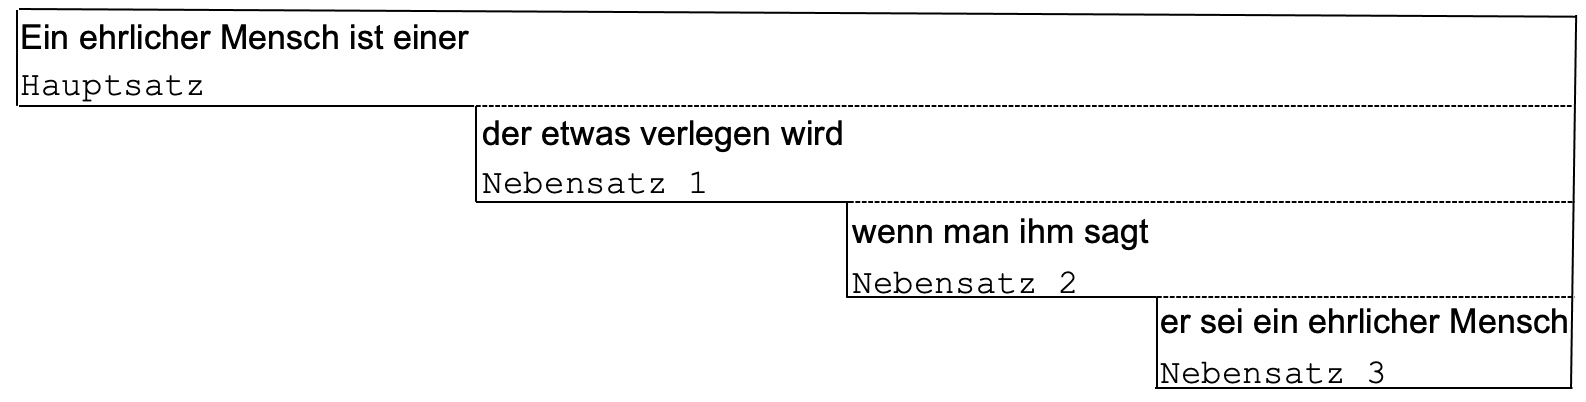
\includegraphics[width=12cm]{figures/Satzbild_Frisch.jpeg}
    %% Abbildung 


\noindent\resizebox{\textwidth}{!}{
	
	\begin{tabular}{  llll |}
		
		\hline
		\multicolumn{1}{ | l }{\makecell[l]{Ein ehrlicher Mensch ist einer \\ \small{\textcolor{gray}{Hauptsatz}}}}  &&& \\ \cline{1-1} \sbdashline{2-4}
		
		& \multicolumn{1}{ | l }{\makecell[l]{der etwas verlegen wird \\ \small{\textcolor{gray}{Nebensatz 1}}}}  && \\ \cline{2-2} \sbdashline{3-4}
		
		&& \multicolumn{1}{ | l }{\makecell[l]{wenn man ihm sagt \\ \small{\textcolor{gray}{Nebensatz 2}}}} & \\ \cline{3-3} \sbdashline{4-4}
		
		&&& \multicolumn{1}{ | l | }{\makecell[l]{er sei ein ehrlicher Mensch \\ \small{\textcolor{gray}{Nebensatz 3}}}} \\ \cline{4-4}
		
	\end{tabular}
}

	

	



    \caption{Satzbild zu (\ref{ea:FrischSatz_2})}
    \label{Abb:Satzbild_Frisch}
\end{figure}

Der Satz beginnt mit dem Hauptsatzgerüst als Teilsatz \textit{ein ehrlicher Mensch ist einer}. In diesen ist der erste komplexe Nebensatz \textit{der etwas verlegen wird, wenn man ihm sagt, er sei ein ehrlicher Mensch} als Attribut zu \textit{einer} integriert. Vom ersten Nebensatz hängt der zweite Nebensatz \textit{wenn man ihm sagt} ab. Dieser sättigt keine Valenzstelle des übergeordneten Prädikats \textit{etwas verlegen wird} (im Sinne von \gq{peinlich berührt werden}), sondern drückt als konditionales Satzadverbial die Bedingung für das Verlegen-Werden-Szenario aus. Der dritte Nebensatz \textit{er sei ein ehrlicher Mensch} sieht zwar durch Verbzweitstellung wie ein Hauptsatz aus. Aber er ist dem zweiten Nebensatz untergeordnet (verkappter Nebensatz). Denn er füllt als Satzobjekt die zweite Valenzstelle des übergeordneten Prädikats \textit{sagt}. 

Zu beachten ist, dass die jeweils tiefer eingebetteten Nebensätze auf höherer Ebene strukturell noch nicht sichtbar sind. Dies zeigt der Voranstellungstest. Der erste Nebensatz ist mit allen tiefer eingebetteten Nebensätzen zusammen mit dem Bezugswort \textit{einer} ein Satzglied im Hauptsatz (\ref{ea:NeSa123_Top}).

\ea \label{ea:NeSa123_Top} \textit{Einer, der etwas verlegen wird, wenn man ihm sagt, er sei ein ehrlicher Mensch}, ist ein ehrlicher Mensch.
\z 


Die Einbettungsebenen werden schrittweise pro Tabellenspalte erfasst. Die Struktur des Hauptsatzes wird ausgehend vom Hauptprädikat in der ersten Spalte analysiert. Das Hauptprädikat wird von der Kopula \textit{ist} in der linken Satzklammer gebildet. Kopulaverben sind zweiwertig und verlangen nach einem Subjekt und einem Subjektsprädikativ als semantisches Zentrum des Prädikats. Da es sich bei \textit{ein ehrlicher Mensch} und \textit{einer, der etwas verlegen wird, wenn man ihm sagt, er sein ein ehrlicher Mensch} um zwei NPs im Nominativ handelt, ist rein formal nicht klar, welche NP das Subjekt und welche das Subjektsprädikativ ist. Im Abschnitt~\ref{subsection:SP und OP} wurde die Funktion der Kopula als Behauptung einer Eigenschafts- oder Klassenzugehörigkeit beschrieben. In dem Satz (\ref{ea:FrischSatz_2}) wird behauptet, dass \textit{einer, der etwas verlegen wird, wenn man ihm sagt, er sei ein ehrlicher Mensch} in die Klasse \textit{ein ehrlicher Mensch} gehört. Folglich bestimmen wir \textit{ein ehrlicher Mensch} als Subjektsprädikativ und \textit{einer, der etwas verlegen wird, wenn man ihm sagt, er sein ehrlicher Mensch} als Subjekt. Diese Analyse wird durch die Umformung mit \textit{gelten als} in (\ref{ea:gelten_als_SP_statt_sein}) bestätigt. Denn mit \textit{gelten} wird das Subjektsprädikativ formal durch \textit{als} gekennzeichnet.

\ea \label{ea:gelten_als_SP_statt_sein} Als ein ehrlicher Mensch gilt einer, der etwas verlegen wird, wenn man ihm sagt, er sei ein ehrlicher Mensch.
\z 

Auch auf der ersten Nebensatz-Ebene bildet ein Kopulaverb, hier \textit{wird}, das Prädikat. Dieses verlangt nach einem Subjekt und einem Subjektsprädikativ. Das Relativpronomen \textit{der} fungiert als Subjekt und \textit{etwas verlegen} als Subjektsprädikativ. Denn es wird behauptet, dass die Eigenschaft \textit{etwas verlegen} auf \textit{der} zutrifft. Der Nebensatz \textit{wenn man ihm sagt, er sei ein ehrlicher Mensch} bildet auf der ersten Nebensatz-Ebene ein Satzglied. Für den Voranstellungstest formen wir den übergeordneten Nebensatz in einen Verbzweitsatz um (\ref{ea:NeSa23_Top}).

\ea \label{ea:NeSa23_Top} \textit{Wenn man ihm sagt, er sein ein ehrlicher Mensch}, wird er etwas verlegen.
\z 

Dieser Nebensatz sättigt keine Valenzstelle, sondern fungiert als konditionales Adverbial.

Der zweite Nebensatz wird mit der Subjunktion \textit{wenn} eingeleitet. Da Subjunktionen weder Satzglied noch Attribut sind, wird in der Tabelle ein Strich gemacht. Die Verbform \textit{sagt} bildet das Prädikat. Ausgehend von seiner Valenz bestimmen wir \textit{man} als dessen Subjekt, \textit{ihm} als Dativobjekt und den verkappten Nebensatz als Satzobjekt. Denn dieser sättigt die Valenzstelle für das, was gesagt wird. Da es sich um ein Satzglied handelt, ist der verkappte Nebensatz bei Umformung des übergeordneten Neben- in einen Hauptsatz voranstellbar (\ref{ea:NeSa3_Top}).

\ea \label{ea:NeSa3_Top} \textit{Er sei ein ehrlicher Mensch}, sagt man ihm.
\z 

Auf der dritten Nebensatz-Ebene wird die interne Struktur des letzten Nebensatzes analysiert. Die Konjunktivform \textit{sei} bildet als Kopula das Prädikat. Das Pronomen \textit{er} fungiert als Subjekt und \textit{ein ehrlicher Mensch} als Subjektsprädikativ.  

Die Analyse wird in der Tabelle~\ref{tab:Frisch_Satz} gezeigt.


\begin{table}
  \centering
  \resizebox{\textwidth}{!}{
  \begin{tabular}{l|l|l|l|l}
   % \lsptoprule
     & Hauptsatz &  1. NeSa-Ebene & 2. NeSa-Ebene  & 3. NeSa-Ebene \\
    \hline
    \textit{Ein} & \multirow{2}{*}{Subjekts-} &  & & \\
    \textit{ehrlicher} & \multirow{2}{*}{prädikativ} & & & \\
    \textit{Mensch} & & & \\ \cline{2-2}
    \textit{ist} & Prädikat  & & & \\ \cline{2-2}
    \textit{einer,} & \multirow{14}{*}{Subjekt} & & \\ \cline{3-3}
    \textit{der} & & Subjekt & &  \\ \cline{3-3}
    \textit{etwas} & & \multirow{1}{*}{Subjekts-} & &\\ 
    \textit{verlegen} & & \multirow{1}{*}{prädikativ} & & \\ \cline{3-3}
    \textit{wird,} & & Prädikat & & \\ \cline{3-4}
    \textit{wenn} & & \multirow{9}{*}{Adverbial} & -- & \\ \cline{4-4}
    \textit{man} & & & Subjekt & \\ \cline{4-4}
    \textit{ihm} & & & Dativobjekt & \\ \cline{4-4}
    \textit{sagt,} & & & Prädikat & \\ \cline{4-5}
    \textit{er} & & & \multirow{5}{*}{Satzobjekt} & Subjekt \\ \cline{5-5}
    \textit{sei} & & & & Prädikat \\ \cline{5-5}
    \textit{ein} & & & & \multirow{2}{*}{Subjekts-} \\ 
    \textit{ehrlicher} & & & & \multirow{2}{*}{prädikativ} \\ 
    \textit{Mensch.} & & & & \\
    \hline 
  %  \lspbottomrule
  \end{tabular}
  }
  \caption{Frisch-Satz}
  \label{tab:Frisch_Satz}
\end{table}


Nun zur Attribut-Ebene: Auf der obersten Ebene ist \textit{ehrlich} ein Adjektivattribut zu \textit{Mensch} und der Nebensatz \textit{der etwas verlegen wird, wenn man ihm sagt, er sei ein ehrlicher Mensch} ist ein Relativsatzattribut zu dem Indefinitpronomen \textit{einer}. 

Auf der ersten Nebensatz-Ebene kann \textit{etwas} im Sinne von \textit{ein bisschen} als Attribut zu dem Adjektiv \textit{verlegen} bestimmt werden. In Analogie zu dem Adverb \textit{sehr} kann es als von der Satzgliedebene abgeleitetes Adverbattribut bezeichnet werden.\footnote{Alternativ kann \textit{etwas} im Sinne von \textit{ein bisschen} als NP analysiert werden. Dann wäre aus dem adverbialen Akkusativ (\textit{etwas}/\textit{den ganzen Tag schlafen}) ein nominales Akkusativattribut geworden.} 

Auf der dritten Nebensatz-Ebene ist wieder \textit{ehrlich} ein Adjektivattribut zu \textit{Mensch}.


\subsection{Beispiel 2}\label{subsection:Bsp2}

Der nächste Satz stammt von Hans Mayer. Auch hier gibt es drei Nebensatz-Ebenen. Das Hauptsatzgerüst und der zweite Nebensatz sind jedoch durch andere Nebensätze \gq{unterbrochen}. Sie sind diskontinuierlich.

\ea \label{ea:Mayer_Satz} Dass sich diese junge Bundesrepublik, aus Rücksichten immer auf Wählerstimmen, nicht dazu entschließen konnte, die verjagten Emigranten, soweit sie noch lebten, zur Rückkehr aufzufordern, gehört, wie ich heute deutlicher spüre als noch vor Jahren, zu den Erbsünden dieses deutschen Teilstaates.\footnote{Hans Mayer: \textit{Wendezeiten}. Frankfurt am Main: Suhrkamp, 1993, S. 50.}
\z 

Erstellen Sie zuerst das Satzbild. Führen Sie danach die Satzgliedanalyse im Tabellenformat durch. Bestimmen Sie im Anschluss daran die Attributrelationen (Attributtyp und Bezugswort).


Kommen wir nun zu den Lösungen: Das Hauptprädikat \textit{gehört} erkennen wir an der Zweitstellung. Das Hauptsatzgerüst lautet \textit{gehört zu den Erbsünden dieses deutschen Teilstaates}. Der erste Nebensatz \textit{dass sich diese junge Bundesrepublik, aus Rücksichten immer auf Wählerstimmen, nicht dazu entschließen konnte} ist direkt dem Hauptsatzprädikat \textit{gehört} untergeordnet, da es der Kern seines Subjekts ist. Der zweite Nebensatz \textit{die verjagten Emigranten zur Rückkehr aufzufordern} hängt vom ersten ab. Denn er drückt das Objekt von \textit{auffordern} aus. Der zweite Nebensatz wird vom dritten Nebensatz \textit{soweit sie noch lebten} unterbrochen. Er hängt vom zweiten Nebensatz ab, denn er drückt die Bedingung dafür aus, unter der die Aufforderung gilt. Der vierte Nebensatz \textit{wie ich heute deutlicher spüre als noch vor Jahren} hängt direkt vom Hauptsatz ab und unterbricht diesen. Er drückt einen Kommentar des Sprechers zur Aussage des Hauptsatzes aus. Die Einbettungsebenen stellen wir in der Abbildung~\ref{Abb:Satzbild_Mayer} im Satzbild\is{Satzbild} dar. 

\begin{figure}
    \centering
    %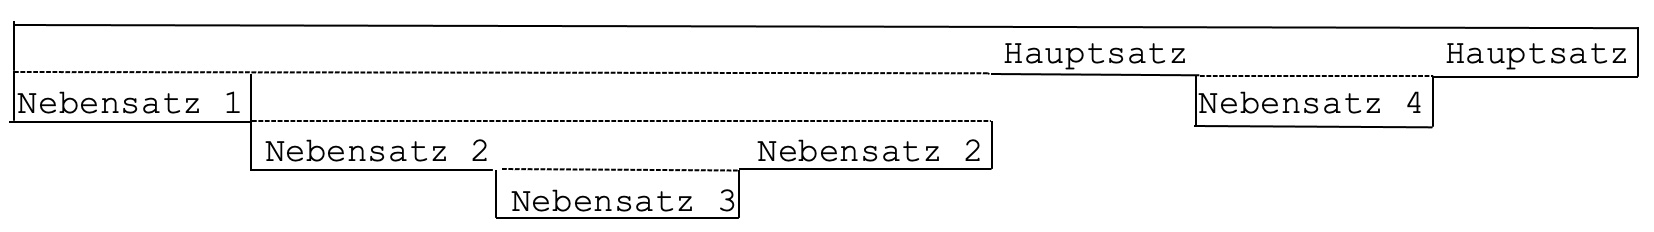
\includegraphics[width=12.5cm]{figures/Satzbild_Mayer.jpg}
    %% Abbildung 


\noindent\resizebox{\textwidth}{!}{
	
	\begin{tabular}{ p{2cm} p{2cm} p{2cm} p{2cm} p{2cm} p{2cm} p{2cm} }
		
		\hline
		
		\multicolumn{1}{ | l}{} & & & & \multicolumn{1}{ l}{\makecell{\small\textcolor{gray}{Hauptsatz}}} & & \multicolumn{1}{ l | }{\makecell{\small\textcolor{gray}{}}} \\ \sbdashline{1-4} \cline{5-5} \sbdashline{6-6} \cline{7-7}
		
		\multicolumn{1}{ | l  }{\makecell{\small\textcolor{gray}{Nebensatz 1}}} & & & \multicolumn{1}{ l | }{} & &
		\multicolumn{1}{ | l | }{\makecell{\small\textcolor{gray}{Nebensatz 4}}} & \\ \cline{1-1} \sbdashline{2-4} \cline{6-6}
		
		& \multicolumn{1}{ | l }{\makecell{\small\textcolor{gray}{Nebensatz 2}}} & &  \multicolumn{1}{ l | }{\makecell{\small\textcolor{gray}{}}} & & & \\ \cline{2-2} \sbdashline{3-3} \cline{4-4}

		& & \multicolumn{1}{ | l | }{\makecell{\small\textcolor{gray}{Nebensatz 3}}} & & & & \\ \cline{3-3} 
			
	\end{tabular}
}

	

    \caption{Satzbild zu (\ref{ea:Mayer_Satz})}
    \label{Abb:Satzbild_Mayer}
\end{figure}

Der Nebensatz im Vorfeld ist zusammen mit den in ihn eingebetteten Nebensätzen \textit{dass sich diese junge Bundesrepublik, aus Rücksichten immer auf Wählerstimmen, nicht dazu entschließen konnte, die verjagten Emigranten, soweit sie noch lebten, zur Rückkehr aufzufordern} das Subjekt des Hauptprädikats \textit{gehört}. Denn er sättigt die erste vom Verb geforderte Ergänzung. Wird sie durch eine NP ausgedrückt, muss sie im Nominativ stehen. Das zeigt die Pronominalisierung des Subjekts durch \textit{das} (\ref{ea:Mayer_Satz_SubjPrn}).

\ea \label{ea:Mayer_Satz_SubjPrn} \textit{Das} gehört, wie ich heute deutlicher spüre als noch vor Jahren, zu den Erbsünden dieses deutschen Teilstaates.
\z 

Ebenfalls als Satzglied innerhalb des Satzganzen fungiert der Nebensatz \textit{wie ich heute deutlicher spüre als noch vor Jahren}. Deshalb kann er, anders als weiterführende Nebensätze, vorangestellt werden (\ref{ea:Mayer_Satz_KAdv_Top}).

\ea \label{ea:Mayer_Satz_KAdv_Top} \textit{Wie ich heute deutlicher spüre als noch vor Jahren}, gehört zu den Erbsünden dieses deutschen Teilstaates, dass sich diese junge Bundesrepublik, aus Rücksichten immer auf Wählerstimmen, nicht dazu entschließen konnte, die verjagten Emigranten, soweit sie noch lebten, zur Rückkehr aufzufordern.
\z 

Dieser Nebensatz sättigt keine Valenzstelle. Durch ihn kommentiert der Schreiber das vom Hauptprädikat ausgedrückte Gehören-Szenario in seinem Geltungsbereich. Es geht um eine so gespürte Tatsache. Wir bestimmen den Nebensatz als Kommentaradverbial (vgl. Abschnitt~\ref{subsection:Adverbial}). Er kann so umgeformt werden, dass er als Hauptsatz den ursprünglichen Haupt- jetzt als Nebensatz einbettet (\ref{ea:Mayer_Satz_KGlied_HS}). Er ist alleine antwortfähig (\ref{ex:Mayer_Satz_KGlied_antwort}) und nicht vom Hauptsatz aus erfragbar (\ref{ex:Mayer_Satz_KGlied_Frage}).

\ea \label{ea:Mayer_Satz_KAdv_Tests}
\ea \label{ea:Mayer_Satz_KGlied_HS} \textit{Ich spüre heute deutlicher als noch vor Jahren}, dass es zu den Erbsünden dieses deutschen Teilstaates gehört, dass sich diese junge Bundesrepublik, aus Rücksichten immer auf Wählerstimmen, nicht dazu entschließen konnte, die verjagten Emigranten, soweit sie noch lebten, zur Rückkehr aufzufordern.
\ex \label{ex:Mayer_Satz_KGlied_antwort} Gehört es zu den Erbsünden dieses deutschen Teilstaates, dass sich diese junge Bundesrepublik, aus Rücksichten immer auf Wählerstimmen, nicht dazu entschließen konnte, die verjagten Emigranten, soweit sie noch lebten, zur Rückkehr aufzufordern? – \textit{Ich spüre das heute deutlicher als vor Jahren} (\textit{so}).
\ex \label{ex:Mayer_Satz_KGlied_Frage} *Wie gehört es zu den Erbsünden dieses deutschen Teilstaates, dass sich diese junge Bunderepublik, aus Rücksichten immer auf Wählerstimmen, nicht dazu entschließen konnte, die verjagten Emigranten, soweit sie noch lebten, zur Rückkehr aufzufordern? – \textit{Ich spüre das heute deutlicher als vor Jahren} (\textit{so}). 
\z 
\z 

Das Prädikat dieses Nebensatzes bildet die Verbform \textit{spüre}. Das Pronomen \textit{ich} fungiert als dessen Subjekt. Ausgehend von der zweiwertigen Valenz ist ein Akkusativobjekt erwartbar. Sprachlich wird dieses aber nicht ausgedrückt. Denn \textit{wie} kodiert normalerweise eine modale Adverbialfunktion. Es gibt zwei Möglichkeiten der Analyse. Entweder verstehen wir das als Adverbial angelegte Satzglied \textit{wie} im Sinne von \gq{was ich heute deutlicher spüre}.\footnote{Dieses Verständnis kann auch bei entsprechendem \textit{wie}-Nebensatz gelten: \textit{Ich spüre, dass/wie es regnet.}} Es gerät in den Sog der offenen Valenzstelle und sättigt diese, als wäre es ein Akkusativobjekt. Oder wir verstehen \textit{spüren} hier absolut als eine Tätigkeit, nicht als Handlung, also einwertig. Dann fungiert \textit{wie}, wie angelegt, als modales Adverbial im Sinne von \gq{auf eine unbestimmte Art spüren}. Wir entscheiden uns für diese Bestimmung, da sie keine Umfunktionierung nötig macht. Das Satzglied \textit{deutlicher als noch vor zehn Jahren} fungiert als modales Adverbial und \textit{heute} als temporales Adverbial. 

Kommen wir nun zu den anderen Nebensätzen. Der Nebensatzkomplex im Vorfeld besteht aus drei Nebensätzen. Der erste Nebensatz lautet \textit{dass sich diese junge Bundesrepublik, aus Rücksichten immer auf Wählerstimmen, nicht dazu entschließen konnte}. Ausgehend von der Valenz von \textit{sich entschließen konnte} bestimmen wir die NP im Nominativ \textit{diese junge Bundesrepublik} als Subjekt und \textit{dazu} als Präpositionalobjekt, worauf weiter unten noch einmal eingegangen wird. Bei \textit{nicht} handelt es sich weder um ein Satzglied noch um den attributiven Teil eines Satzglieds. Dies wird in der Analyse durch einen Strich gekennzeichnet. 

Bei \textit{aus Rücksichten immer auf Wählerstimmen} handelt es sich um ein eingeschobenes kausales Adverbial, das den Grund dafür angibt, warum sich diese Bundesrepublik nicht zu etwas entschließen konnte. Es bezieht sich direkt auf das Prädikat \textit{sich entschließen konnte}. Dies bestätigt der Voranstellungstest in (\ref{ex:Mayer_Satz_aus_Rücksichten_Top}), wenn der einbettende Nebensatz in einen Hauptsatz umformuliert wird (\ref{ea:Mayer_Satz_aus_Rücksichten_HS}). 

\ea \label{ea:Mayer_Satz_aus_Rücksichten_Top_HS} 
\ea \label{ea:Mayer_Satz_aus_Rücksichten_HS} Diese junge Bundesrepublik konnte sich, aus Rücksichten immer auf Wählerstimmen, nicht dazu entschließen.
\ex \label{ex:Mayer_Satz_aus_Rücksichten_Top} \textit{Aus Rücksichten immer auf Wählerstimmen} konnte sich diese junge Bundesrepublik nicht dazu entschließen.
\z 
\z 

Das kausale Adverbial \textit{aus Rücksichten immer auf Wählerstimmen} ist komplex, kann aber nicht im Rahmen der Satzgliedanalyse \gq{aufgedröselt} werden. Es besteht nämlich intern nicht aus Satzgliedern, da es kein Prädikat gibt.

Die Proform \textit{dazu} im ersten Nebensatz zeigt wie ein Korrelat (vgl. Abschnitt~\ref{subsection:Korrelat}) die Sättigung der zweiten Valenzstelle des Prädikats an. Das Prädikat \textit{sich entschließen konnte} fordert eine zweite Ergänzung in Form einer PP mit \textit{zu}. Darüber hinaus kann \textit{dazu} mit Betonung auf \textit{da} auf den als Attribut fungierenden Nebensatzkomplex \textit{die verjagten Emigranten, soweit sie noch lebten, zur Rückkehr aufzufordern} zeigen. Als Test gilt wieder die gemeinsame Voranstellbarkeit (\ref{ea:ea:Mayer_Satz_dazu_zuINF_Top}) bei Umformung in einen Hauptsatz.

\ea \label{ea:ea:Mayer_Satz_dazu_zuINF_Top} \textit{Dazu, die Emigranten, soweit sie noch lebten, zur Rückkehr aufzufordern}, konnte sich diese junge Bundesrepublik nicht entschließen.
\z 

In diesem Fall ist \textit{dazu} der Kern des Präpositionalobjekts, zu dem der Nebensatz als Attribut gehört. Wird hingegen \textit{dazu} mit Betonung auf \textit{zu} gelesen, dann müsste es als Korrelat zum Satzobjekt \textit{die Emigranten, soweit sie noch lebten, zur Rückkehr aufzufordern} analysiert werden. Beide Analysen wären korrekt.  

Die zweite nebensatzähnliche Struktur \textit{die Emigranten zur Rückkehr aufzufordern} wird durch die Infinitiv-Konstruktion (vgl. \ref{subsection:NebensatzähnlicheK}) mit \textit{aufzufordern} als Prädikat gebildet. Da Infinitive die erste verbale Ergänzung im Nominativ nicht ausdrücken können, gibt es kein Subjekt. Der Infinitiv \textit{aufzufordern} verlangt jedoch nach einer Ergänzung im Akkusativ und nach einer Ergänzung mit der Präposition \textit{zu}. Folglich fungieren \textit{die Emigranten} als Akkusativobjekt und \textit{zur Rückkehr} als Präpositionalobjekt.

Die Infinitiv-Konstruktion ist durch den Nebensatz \textit{soweit sie noch lebten} unterbrochen. Der Begriff \textit{Einbettung} wird hier plastisch. Der dritte Nebensatz \textit{soweit sie noch lebten} liegt innerhalb der zweiten nebensatzähnlichen Konstruktion. Er sättigt keine Valenzstelle des einbettenden Prädikats \textit{aufzufordern}, sondern drückt als konditionales Adverbial die Bedingung für jene Aufforderung aus. Dass es sich um ein Adverbial und damit um ein Satzglied handelt, wird durch den Voranstellungstest in (\ref{ex:Mayer_Satz_soweit_Top}) bei Umformulierung in einen Hauptsatz (\ref{ea:ea:Mayer_Satz_soweit_in_HS}) untermauert.

\ea \label{ea:ea:Mayer_Satz_soweit_Top_HS} 
\ea \label{ea:ea:Mayer_Satz_soweit_in_HS} Diese junge Bundesrepublik forderte die Emigranten, soweit sie noch lebten, nicht zur Rückkehr auf.
\ex \label{ex:Mayer_Satz_soweit_Top} \textit{Soweit sie noch lebten}, forderte diese junge Bundesrepublik die Emigranten nicht zur Rückkehr auf.\footnote{Allerdings bekommt dieses Satzgefüge eine weitere Lesart, nämlich dass die Emigranten nicht zur Rückkehr aufgefordert wurden, weil sie noch lebten. Unser Weltwissen arbeitet bei der sinnvollen Interpretation mit. Im Präteritum \textit{soweit sie noch lebten} ergibt sich Plausibilität der konditionalen Kodierung durch kausale Interpretation.}
\z 
\z 

Das Zentrum des eingebetteten Nebensatzes bildet die Verbform \textit{lebten} als Prädikat. Es verlangt nach einer Ergänzung im Nominativ. Das Pronomen \textit{sie} sättigt diese Valenzstelle und fungiert als Subjekt. Durch \textit{noch} wird keine Valenzstelle gesättigt. Es drückt zeitliche Aspekte des Leben-Szenarios aus und ist somit ein temporales Adverbial. Die Subjunktion \textit{soweit} ist weder Satzglied noch Teil eines Satzglieds und wird daher nicht bestimmt. 

Die Satzgliedanalyse wird in der Tabelle~\ref{tab:Mayer_Satz} dargestellt. Die Spalten entsprechen wieder den Ebenen des Satzbildes, wenn dieses um 90 Grad nach links gedreht würde.

\begin{table}
%\scriptsize  
  \centering
  \resizebox{\textwidth}{!}{
  \begin{tabular}{l|l|l|l|l}
   % \lsptoprule
     &  Hauptsatz  &  1. NeSa-Ebene &  2. NeSa-Ebene &  3. NeSa-Ebene \\
    \hline
    \textit{Dass} & \multirow{29}{*}{Subjekt} & -- & & \\ \cline{3-3}
    \textit{sich} & & Prädikat & & \\ \cline{3-3}
    \textit{diese} & & \multirow{3}{*}{Subjekt} & & \\  
    \textit{junge} &  & & & \\ 
    \textit{Bundesrepublik,} & & & & \\ \cline{3-3}
    \textit{aus} & & \multirow{5}{*}{Adverbial} \\
    \textit{Rücksichten} & & & & \\
    \textit{immer} & & & & \\ 
    \textit{auf} & & & & \\ 
    \textit{Wählerstimmen,} & & & & \\ \cline{3-3}
    \textit{nicht} & & -- & & \\ \cline{3-3}
    \textit{dazu} & & Präpositionalobjekt & & \\ \cline{3-3}
    \textit{entschließen} & & \multirow{2}{*}{Prädikat} & & \\ 
    \textit{konnte,} & & & & \\ \cline{3-4}
    \textit{die} & & \multirow{10}{*}{Präpositionalobjekt} & \multirow{3}{*}{Akkusativobjekt} & \\
    \textit{verjagten} & &  &  & \\
    \textit{Emigranten,} & & & & \\ \cline{4-5}
    \textit{soweit} & & & \multirow{4}{*}{Adverbial} & -- \\ \cline{5-5}
    \textit{sie} & & & & Subjekt \\ \cline{5-5}
    \textit{noch} & & & & Adverbial \\ \cline{5-5}
    \textit{lebten,} & & & & Prädikat \\ \cline{4-5}
    \textit{zur} & & & \multirow{2}{*}{Präpositionalobjekt} & \\
    \textit{Rückkehr} & & & & \\ \cline{4-4}
    \textit{aufzufordern,} & & & Prädikat & \\ \cline{2-4} 
    \textit{gehört,} & Prädikat & -- & & \\ \cline{2-3}
    \textit{wie} & \multirow{10}{*}{Kommentaradverbial} & Adverbial & & \\ \cline{3-3}
    \textit{ich} & & Subjekt & & \\ \cline{3-3}
    \textit{heute} & & Adverbial 1 & & \\ \cline{3-3}
    \textit{deutlicher} & & Adverbial 2 & & \\ \cline{3-3}
    \textit{spüre} & & Prädikat & & \\ \cline{3-3}
    \textit{als} & & \multirow{5}{*}{Adverbial 2} & & \\ 
    \textit{noch} & & & & \\
    \textit{vor} & & & & \\ 
    \textit{zehn} & & & & \\ 
    \textit{Jahren,} & & & & \\ \cline{2-3}
    \textit{zu} & \multirow{6}{*}{Präpositionalobjekt} & & & \\ 
    \textit{den} & & & & \\
    \textit{Erbsünden} & & & & \\ 
    \textit{dieses} & & & & \\ 
    \textit{deutschen} & & & & \\ 
    \textit{Teilstaates.} & & & & \\
    \hline 
   % \lspbottomrule
  \end{tabular}
  }
  \caption{Diskontinuierliche Sätze durch Einbettung}
  \label{tab:Mayer_Satz}
\end{table}

Kommen wir nun zu den Attributen: Auf der ersten Ebene ist innerhalb des Präpositionalobjektes die NP \textit{dieses deutschen Teilstaates} ein Genitivattribut zu \textit{Erbsünde}. Innerhalb des Attributs \textit{dieses deutschen Teilstaates} ist \textit{deutschen} ein Adjektivattribut zu \textit{Teilstaates}.

Auf der ersten Nebensatz-Ebene ist die PP \textit{auf Wählerstimmen} ein Präpositionalattribut zu \textit{Rücksichten}. Das Adverb \textit{immer} fungiert als Adverbphrase (vgl. Abschnitt~\ref{section:Adverbphrase}) typischerweise als Adverbial. Da es hier kein Prädikat gibt, ist diese Funktion ausgeschlossen. Analog zu Fokuspartikeln wie \textit{besonders} in \textit{besonders auf Wählerstimmen} analysieren wir \textit{immer} als Adverbattribut zu der PP \textit{auf Wählerstimmen}.\footnote{Die syntaktische Attributbeziehung innerhalb von \textit{immer auf Wählerstimmen} ist analog zur Modifikation lokaler PPs wie \textit{direkt vor der Kreuzung} zu verstehen.}

Da wir \textit{dazu} als Kern des Präpositionalobjekts (und nicht, was auch möglich wäre, als Korrelat zum Satzobjekt) analysiert haben, fungiert die Infinitivkonstruktion \textit{die verjagten Emigranten, soweit sie noch lebten, zur Rückkehr aufzufordern} als Attribut zu \textit{dazu}. Auch hier handelt es sich um eine Umfunktionierung von der Satzgliedebene auf die Ebene der Wortgruppe.

Die Vergleichsphrase \textit{als noch vor zehn Jahren} ist ein Attribut der Komparativform \textit{deutlicher} und damit Teil des Adverbials. 

Auf der zweiten Nebensatz-Ebene ist \textit{verjagten} ein Adjektivattribut zu \textit{Emigranten}. Auf der dritten Nebensatz-Ebene gibt es keine Attribute.


\subsection{Beispiel 3}\label{subsection:Bsp3}

Nun analysieren wir den folgenden Satz aus \textit{Max und Moritz} von Wilhelm Busch.

\ea \label{ea:Busch_Satz} Als die gute Witwe Bolte sich von ihrem Schmerz erholte, dachte sie so hin und her, dass es wohl das beste wär, die Verstorbenen, die hienieden schon so frühe abgeschieden, ganz im Stillen und in Ehren gut gebraten zu verzehren.\footnote{Wilhelm Busch: \textit{Max und Moritz. Eine Bubengeschichte in sieben Streichen}. [1865]. Göttingen: Literatur- und Wissenschaftsverlag, 2019, S. 7.}
\z 

Erstellen Sie zuerst das Satzbild. Führen Sie danach die Satzgliedanalyse im Tabellenformat durch. Bestimmen Sie im Anschluss daran die Attributrelationen (Attributtyp und Bezugswort).


Kommen wir nun zu den Lösungen: Das Hauptprädikat \textit{dachte} erkennen wir an der Zweitstellung. Das Hauptsatzgerüst lautet \textit{dachte sie so hin und her}. Der erste Nebensatz \textit{als die gute Witwe Bolte sich von ihrem Schmerz erholte} ist direkt dem Hauptsatz untergeordnet, da er die Zeit des \textit{Denkens} ausdrückt. Den Inhalt des \textit{Denkens} drückt der zweite Nebensatz \textit{dass es wohl das beste wär} aus und ist somit direkt dem Hauptsatzprädikat untergeordnet. Der dritte Nebensatz \textit{die Verstorbenen ganz im Stillen und in Ehren gut gebraten zu verzehren} ist direkt dem zweiten Nebensatz untergeordnet. Denn er drückt das aus, was das \textit{beste wär}. Der vierte Nebensatz \textit{die hienieden schon so frühe abgeschieden} unterbricht den dritten Nebensatz, in den er eingebettet ist. Denn er hängt direkt von \textit{die Verstorbenen} ab.

Die Einbettungsebenen der Nebensätze stellen wir in der Abbildung~\ref{Abb:Satzbild_Max_Moritz} im Satzbild\is{Satzbild} dar.

\begin{figure}
    \centering
    %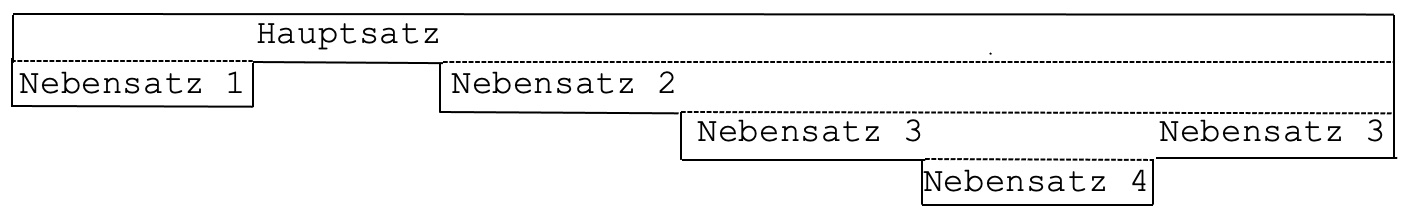
\includegraphics[width=12.5cm]{figures/Satzbild_Max_Moritz.jpeg}
    %% Abbildung 


\noindent\resizebox{\textwidth}{!}{
	
	\begin{tabular}{ p{2cm} p{2cm} p{2cm} p{2cm} p{2cm} p{2cm} }
		
		\hline
		
		\multicolumn{1}{ | l}{} &
		\multicolumn{1}{ l }{\makecell[l]{\small\textcolor{gray}{Hauptsatz}}} & & & &
		\multicolumn{1}{ l | }{} \\ 
		\sbdashline{1-1} \cline{2-2} \sbdashline{3-6} 
		
		\multicolumn{1}{ | l | }{\makecell[l]{\small\textcolor{gray}{Nebensatz 1}}} & &  
		\multicolumn{1}{ | l  }{\makecell[l]{\small\textcolor{gray}{Nebensatz 2}}} & & & 
		\multicolumn{1}{ l | }{} \\
		 \cline{1-1} \cline{3-3} \sbdashline{4-6} 
		 
		& & &  \multicolumn{1}{ | l }{\makecell[l]{\small\textcolor{gray}{Nebensatz 3}}} & &  
		\multicolumn{1}{ l | }{\makecell[l]{\small\textcolor{gray}{}}} \\
		 \cline{4-4} \sbdashline{5-5}  \cline{6-6}
		 
		 & & & & \multicolumn{1}{ | l | }{\makecell[l]{\small\textcolor{gray}{Nebensatz 4}}} & \\
		 \cline{5-5} 
			
	\end{tabular}
}


    \caption{Satzbild zu (\ref{ea:Busch_Satz})}
    \label{Abb:Satzbild_Max_Moritz}
\end{figure}

Das Prädikat des Hauptsatzes ist \textit{dachte}. Das Pronomen \textit{sie} sättigt als NP im Nominativ die erste Valenzstelle von \textit{dachte} und fungiert als Subjekt. Die koordinierte Adverbphrase \textit{so hin und her} sättigt keine Valenzstelle, sondern drückt im weiteren Sinne eine Art und Weise des Denkens aus.\footnote{Es handelt sich um eine bildliche Übertragung von Bewegungssituationen wie \textit{hin und her laufen}. Die ursprüngliche Bedeutung \gq{ständig die Richtung wechselnd} wird metaphorisch als \gq{gründlich, alles erwägend} verstanden}. Es handelt sich um ein modales Adverbial. Die Erststellfähigkeit (\ref{ea:Busch_Satz_hinher_Top}) spricht für den Satzgliedstatus.

\ea \label{ea:Busch_Satz_hinher_Top} \textit{So hin und her} dachte sie, dass\ldots{} 
\z 

Denkbar wäre jedoch auch, \textit{hin} und \textit{her} als Teile des Prädikats zu bestimmen. Auch diese können vorangestellt werden. Dagegen spricht, dass es für sich genommen weder ein *\textit{Hindenken} noch ein *\textit{Herdenken} gibt. \textit{Hin und her} bildet eine im Satz bewegliche Phrase, die über Bewegungsverben hinaus metaphorisch gebraucht werden kann. Vor allem spricht gegen die Bestimmung als Prädikatsteil, dass \textit{hin und her} auch mit Verben, die bereits eine Partikel oder ein Präfix enthalten, gebraucht werden kann wie in \textit{etwas hin und her abwägen} oder \textit{etwas hin und her überlegen}.    
 
Das Hauptprädikat \textit{dachte} verlangt nach einer zweiten Ergänzung, die den Inhalt des Denkens typischerweise durch einen Nebensatz ausdrückt. Der Nebensatzkomplex \textit{dass es wohl das beste wär, die Verstorbenen, die hienieden schon so frühe abgeschieden, ganz im Stillen und in Ehren gut gebraten zu verzehren} sättigt diese Valenzstelle und ist damit ein Satzobjekt. Hierfür sprechen die gemeinsame Voranstellbarkeit (\ref{ea:Busch_Satz_Satzobj_Top}), die Pronominalisierbarkeit (\ref{ex:Busch_Satz_Satzobj_Pronomen}) und Erfragbarkeit durch ein Fragepronomen (\ref{ex:Busch_Satz_Satzobj_Frage}).

\ea \label{ea:Busch_Satz_Satzobj}
\ea \label{ea:Busch_Satz_Satzobj_Top} \textit{Dass es wohl das beste wär, die Verstorbenen, die hienieden schon so frühe abgeschieden, ganz im Stillen und in Ehren gut gebraten zu verzehren}, dachte die gute Witwe Bolte so hin und her, als sie sich von ihrem Schmerz erholte.\footnote{Innerhalb des Hauptsatzes muss jetzt das Subjekt \textit{sie} durch \textit{die gute Witwe Bolte} ersetzt werden. Denn das Pronomen \textit{sie} soll auf die referierende (in die Welt zeigende) NP \textit{die gute Witwe Bolte} verweisen. Dieses Verweisen vom Pronomen auf eine NP (Phorik) funktioniert nur, wenn das Pronomen und die NP nicht auf gleicher und wenn das Pronomen nicht auf einer höheren Strukturposition als die NP steht. Eine höhere Strukturposition bedeutet hier: Das Pronomen kann nicht aus dem Hauptsatz auf eine NP im folgenden Nebensatz verweisen: *\textit{sie dachte das so hin und her, als die gute Witwe Bolte sich von ihrem Schmerz erholte}. Wenn das Pronomen im Nebensatz und somit strukturtiefer steht, dann kann es auch bei Voranstellung (Thema-Stellung) auf die NP im Hauptsatz verweisen: \textit{als sie sich vom Schmerz erholte, dachte die gute Witwe Bolte das so hin und her}. Dieses Phänomen wird in der Linguistik unter dem Stichwort \textit{Koreferenz} diskutiert. Cf. \citet[93--104]{FanselowFelix1993} und \citet[109--115]{Welke1993}.} 
\ex \label{ex:Busch_Satz_Satzobj_Pronomen} Als die gute Witwe Bolte sich von ihrem Schmerz erholte, dachte sie \textit{das} so hin und her.
\ex \label{ex:Busch_Satz_Satzobj_Frage} \textit{Was} dachte die gute Witwe Bolte so hin und her,  als sie sich von ihrem Schmerz erholte?
\z 
\z 

Vor dem Hauptprädikat \textit{dachte} erwarten wir ein Satzglied. Der Nebensatz \textit{als die gute Witwe Bolte sich von ihrem Schmerz erholte} sättigt keine Valenzstelle von \textit{dachte}. Er drückt ein Szenario aus, das zeitgleich zum Szenario des Hauptsatzes stattfindet. Es handelt sich um ein temporales Adverbial. Das Reflexivpronomen ist Teil des Prädikats \textit{sich erholte}, denn es sättigt keine Valenzstelle (vgl. Abschnitt~\ref{subsection:Reflexiva}). Es ist zweiwertig. Die NP im Nominativ \textit{die gute Witwe Bolte} fungiert als Subjekt und die PP \textit{von ihrem Schmerz} als Präpositionalobjekt (vgl. Abschnitt~\ref{subsection:Pobj}).

Jetzt beschäftigen wir uns mit dem als Satzobjekt fungierenden Nebensatzkomplex: \textit{dass es wohl das beste wär, die Verstorbenen, die hienieden schon so frühe abgeschieden, ganz im Stillen und in Ehren gut gebraten zu verzehren}. Der erste Nebensatz \textit{dass es wohl das beste wär} enthält ein Korrelat. \textit{Es} zeigt an, dass ein Nebensatz in Objekt- oder Subjektfunktion folgt. Bei \textit{wär} handelt es sich um eine Konjunktivform (II) der Kopula \textit{sein}. Ihre Ergänzung ist das Subjektsprädikativ \textit{das beste}. Das Korrelat \textit{es} steht also im Nominativ und zeigt auf die folgende Infinitivkonstruktion in Subjektfunktion. Diese Funktion übernimmt der ganze folgende Komplex \textit{die Verstorbenen, die hienieden schon so frühe abgeschieden, ganz im Stillen und in Ehren gut gebraten zu verzehren}. Dass es sich in Bezug auf \textit{das beste sein} um \textit{ein} Satzglied handelt, zeigt bei Umformung in einen Hauptsatz (\ref{ea:Busch_Satz_beste_wär_Inf_HS}) die Voranstellung (\ref{ex:Busch_Satz_beste_wär_Inf_Top}).

\ea \label{ea:Busch_Satz_beste_wär_Inf}
\ea \label{ea:Busch_Satz_beste_wär_Inf_HS} Wohl wäre es das beste, die Verstorbenen, die hienieden schon so frühe abgeschieden, ganz im Stillen und in Ehren gut gebraten zu verzehren.
\ex \label{ex:Busch_Satz_beste_wär_Inf_Top} \textit{Die Verstorbenen, die hienieden schon so frühe abgeschieden, ganz im Stillen und in Ehren gut gebraten zu verzehren}, wäre wohl das beste.
\z 
\z 

Dass es sich bei \textit{es} tatsächlich um ein Subjekt-Korrelat und nicht um das Subjekt handelt, wird in (\ref{ex:Busch_Satz_beste_wär_Inf_Top}) deutlich. Bei Voranstellung des Subjektsatzes entfällt \textit{es}. 

Bei der Umformung in einen Hauptsatz (\ref{ea:Busch_Satz_beste_wär_Inf_HS}) haben wir \textit{wohl} ins Vorfeld gestellt. So sehen wir erstens, dass \textit{es} kein reiner Vorfeld-Platzhalter (vgl. Abschnitt~\ref{subsection:Vorfeld}) ist und dass dieses \textit{wohl} ein Satzglied ist. Wir bestimmen \textit{wohl} als Kommentaradverbial (vgl. Abschnitt~\ref{subsection:Adverbial}). Denn es räumt wie \textit{wahrscheinlich} oder \textit{bestimmt} Zweifel bezüglich der Geltung des gesamten Szenarios aus. Es kann in einen Hauptsatz umgeformt werden, der den ursprünglich einbettenden Satz zum Nebensatz macht (\ref{ea:Busch_Satz_beste_wär_wohl_HS}) und es ist nicht wie andere Adverbiale erfragbar (\ref{ex:Busch_Satz_beste_wär_wohl_*Frage}).


\ea \label{ea:Busch_Satz_beste_wär_wohl}
\ea [] {Es ist wohl so, dass es das beste wär, die Verstorbenen, die hienieden schon so frühe abgeschieden, ganz im Stillen und in Ehren gut gebraten zu verzehren.}\label{ea:Busch_Satz_beste_wär_wohl_HS}
\ex [*] {\textit{Wie} wäre es das beste, die Verstorbenen, die hienieden schon so frühe abgeschieden, ganz im Stillen und in Ehren gut gebraten zu verzehren?  -- Wohl.}\label{ex:Busch_Satz_beste_wär_wohl_*Frage}
\z 
\z 

Bei dem Subjekt \textit{die Verstorbenen, die hienieden schon so frühe abgeschieden, ganz im Stillen und in Ehren gut gebraten zu verzehren} handelt es sich um eine satzwertige \textit{zu}-Infinitiv-Konstruktion (vgl. Abschnitt~\ref{subsection:NebensatzähnlicheK}). Deren Prädikat bildet \textit{zu verzehren}. Da es sich um einen Infinitiv handelt, kann das mitzudenkende Subjekt formal nicht ausgedrückt werden. Die zweite, obligatorisch zu besetzende Valenzstelle von \textit{verzehren} wird durch \textit{die Verstorbenen, die hienieden schon so frühe abgeschieden} als Akkusativobjekt gesättigt. Dass es sich auf dieser Ebene um \textit{ein} Satzglied handelt, wird bei Umformung in einen Hauptsatz (\ref{ea:Busch_Satz_zu_verzehren_HS}) durch Voranstellung (\ref{ex:Busch_Satz_zu_verzehren_Top}) deutlich.

\ea \label{ea:Busch_Satz_zu_verzehren_HS_TOP}
\ea \label{ea:Busch_Satz_zu_verzehren_HS} Sie will die Verstorbenen, die hienieden schon so frühe abgeschieden, ganz im Stillen und in Ehren gut gebraten verzehren.
\ex \label{ex:Busch_Satz_zu_verzehren_Top} {Die Verstorbenen, die hienieden schon so frühe abgeschieden}, will sie ganz im Stillen und in Ehren gut gebraten verzehren.
\z 
\z 

Die koordinierten PPs \textit{ganz im Stillen und in Ehren} bilden ebenfalls ein Satzglied. Der Komplex ist voranstellbar (\ref{ea:Busch_Satz_zu_verzehren_im_Stillen_Top}) und erfragbar (\ref{ex:Busch_Satz_zu_verzehren_im_Stillen_Frage}).

\ea \label{ea:Busch_Satz_zu_verzehren_im_Stillen}
\ea \label{ea:Busch_Satz_zu_verzehren_im_Stillen_Top} \textit{Ganz im Stillen und in Ehren} will sie die Verstorbenen, die hienieden schon so frühe abgeschieden, gut gebraten verzehren.
\ex \label{ex:Busch_Satz_zu_verzehren_im_Stillen_Frage} \textit{Wie} will sie die Verstorbenen, die hienieden schon so frühe abgeschieden,  gut gebraten verzehren? -- Ganz im Stillen und in Ehren.
\z 
\z 

Der Komplex sättigt keine Valenzstelle von \textit{zu verzehren}. Er drückt die Art und Weise des Verzehren-Szenarios aus. Es handelt sich um ein modales Adverbial.

Bei \textit{gut gebraten} handelt es sich um eine satzwertige Partizipial-Konstruktion (vgl. Abschnitt~\ref{subsection:NebensatzähnlicheK}). Wir bestimmen sie als Satzglied. Dafür spricht ihre Voranstellbarkeit (\ref{ea:Busch_Satz_gut_gebraten_TOP}).

\ea \label{ea:Busch_Satz_gut_gebraten_TOP} \textit{Gut gebraten} will sie die Verstorbenen, die hienieden schon so frühe abgeschieden, verzehren.
\z 

Um welche Satzgliedfunktion handelt es sich? Die Partizipial-Konstruktion sättigt weder eine Valenzstelle des Prädikats \textit{zu verzehren} noch spezifiziert sie wie Adverbiale das Verzehren-Szenario. Sie weist dem Akkusativobjekt \textit{die Verstorbenen, die hienieden schon so frühe abgeschieden} die Eigenschaft \textit{gut gebraten} für die Zeit des Verzehrens zu. Diese Funktion kommt freien Prädikativen (vgl. Abschnitt~\ref{subsection:freiePräd}) zu. Hier handelt es sich um ein freies Objekstprädikativ. Der besondere Bezug zum Objekt zeigt sich in Stellungseigenschaften. Das freie Prädikativ folgt bei Nebensatzstellung typischerweise seinem Bezugswort. In (\ref{ea:Busch_Satz_gut_gebraten_Obj_Adjazenz}) folgt \textit{gut gebraten} dem Objekt. In (\ref{ex:Busch_Satz_gut_gebraten_Subj_Adjazenz}) müssten wir die Partizipial-Konstruktion als freies Subjektsprädikativ verstehen, also dass Witwe Bolte zum Zeitpunkt des Verzehrens gut gebraten ist.

\ea \label{ea:Busch_Satz_gut_gebraten_FP}
\ea \label{ea:Busch_Satz_gut_gebraten_Obj_Adjazenz} weil die gute Witwe Bolte die Verstorbenen \textit{gut gebraten} verzehren will.
\ex \label{ex:Busch_Satz_gut_gebraten_Subj_Adjazenz} weil die gute Witwe Bolte \textit{gut gebraten} die Verstorbenen verzehren will
\z 
\z 

Intern besteht das freie Prädikativ aus dem Prädikat \textit{gebraten} und dem nicht-valenzsättigenden Adverbial \textit{gut}.

Nun muss noch die Funktion des eingebetteten Nebensatzes \textit{die hienieden schon so frühe abgeschieden} bestimmt werden. Es handelt sich formal um einen elliptischen Relativsatz. Elliptisch ist er, weil das finite Hilfsverb \textit{sind} zum Perfektausdruck \textit{abgeschieden sind} in der Bedeutung von \textit{gestorben/verschieden sind} ausgelassen wurde. Seine Funktion ist die nähere Bestimmung von \textit{die Verstorbenen}. Er ist kein Satzglied, sondern als Attribut Teil des Akkusativobjekts, wofür auch die gemeinsame Voranstellung in (\ref{ex:Busch_Satz_zu_verzehren_Top}) spricht. Intern besteht er aus \textit{die} in Subjektfunktion, \textit{hienieden} als lokales Adverbial und \textit{schon so frühe} als temporales Adverbial zum Prädikat \textit{abgeschieden} (\textit{sind}). 

Die Satzgliedanalyse wird in der Tabelle~\ref{tab:Busch_Satz} dargestellt.

\begin{table}
%\scriptsize  
  \centering
  \resizebox{\textwidth}{!}{
  \begin{tabular}{l|l|l|l|l}
   % \lsptoprule
      &  Haupsatz  &  1. NeSa-Ebene  &  2. NeSa-Ebene  &  3. NeSa-Ebene  \\
    \hline
    \textit{Als} & \multirow{10}{*}{Adverbial} & -- & & \\ \cline{3-3}
    \textit{die} & & \multirow{3}{*}{Subjekt} & & \\ 
    \textit{gute} & & & & \\ 
    \textit{Witwe} & & & & \\
    \textit{Bolte} & & & & \\ \cline{3-3}
    \textit{sich} & & Prädikat & & \\ \cline{3-3}
    \textit{von} & & \multirow{3}{*}{Präpositionalobjekt} & & \\
    \textit{ihrem} & & & & \\ 
    \textit{Schmerz} & & & & \\ \cline{3-3}
    \textit{erholte,} & & Prädikat & & \\ \cline{2-3}
    \textit{dachte} & Prädikat & & & \\ \cline{2-2}
    \textit{sie} & Subjekt & & & \\ \cline{2-2}
    \textit{so} & \multirow{4}{*}{Adverbial} & & & \\ 
    \textit{hin} & & & & \\ 
    \textit{und} & & & & \\ 
    \textit{her,} & & & & \\ \cline{2-3}
    \textit{dass} & \multirow{23}{*}{Satzobjekt} & -- & & \\ \cline{3-3}
    \textit{es} & & Subjekt-Korrelat & & \\ \cline{3-3}
    \textit{wohl} & & Kommentaradverbial & & \\ \cline{3-3}
    \textit{das} & & \multirow{2}{*}{Subjektsprädikativ} & & \\ 
    \textit{beste} & & & & \\ \cline{3-3}
    \textit{wär,} & & Prädikat & & \\ \cline{3-4}
    \textit{die} & & \multirow{18}{*}{Subjekt} & \multirow{8}{*}{Akkusativobjekt} & \\ 
    \textit{Verstorbenen,} & & & & \\ \cline{5-5}
    \textit{die} & & & & Subjekt \\ \cline{5-5}
    \textit{hienieden} & & & & Adverbial \\ \cline{5-5}
    \textit{schon} & & & & \multirow{3}{*}{Adverbial} \\ 
    \textit{so} & & & & \\ 
    \textit{frühe} & & & & \\ \cline{5-5}
    \textit{abgeschieden,} & & & & Prädikat \\ \cline{4-5}
    \textit{ganz} & & & \multirow{6}{*}{Adverbial} & \\ 
    \textit{im} & & & & \\ 
    \textit{Stillen} & & & & \\ 
    \textit{und} & & & & \\ 
    \textit{in} & & & & \\ 
    \textit{Ehren} & & & & \\ \cline{4-5}
    \textit{gut} & & & \multirow{2}{*}{freies Prädikativ} & Adverbial \\ \cline{5-5}
    \textit{gebraten} & & & & Prädikat \\ \cline{4-5}
    \textit{zu} & & & \multirow{2}{*}{Prädikat} & \\ 
    \textit{verzehren.} & & & & \\
    \hline 
  %  \lspbottomrule
  \end{tabular}
  }
  \caption{Max-und-Moritz-Satz}
  \label{tab:Busch_Satz}
\end{table}

Abschließend bestimmen wir die Attribute und ihre Bezugswörter. Auf der Ebene des Satzganzen könnte das komplexe Adverbial \textit{so hin und her} in \textit{hin und her} als koordiniertes Bezugsadverb und \textit{so} als Adverbattribut bestimmt werden. Dafür spricht die Weglassbarkeit von \textit{so}. Allerdings bestimmt dieses \textit{so} die Bedeutung von \textit{hin und her} nicht näher. Dieses \textit{so} ist eher eine Abtönungspartikel (vgl. Abschnitt~\ref{subsubsection:Abtönung}). Sie verleiht der gesamten Aussage \textit{hin und her denken} etwas Vages wie in \textit{Ich ging im Walde/So für mich hin}.\footnote{Die Zeilen stammen aus dem Gedicht \textit{Gefunden} von Goethe. Diese abtönende Funktion ist zu unterscheiden von dem betonbaren Adverb \textit{so}, das auf eine vorher erwähnte Art und Weise wie in \textit{so mache ich das auch} verweist. Ebenfalls muss die Abtönungspartikel von dem modifizierenden \textit{so} im Sinne von \textit{ungefähr} wie in \textit{wir treffen uns so um 17 Uhr} unterschieden werden.} Deshalb bestimmen wir es nicht attributiv.


Auf der ersten Nebensatz-Ebene ist das Subjekt \textit{die gute Witwe Bolte} eine komplexe NP. Ihr Kopf ist \textit{Witwe}. Das Adjektiv \textit{gute} fungiert als Adjektivattribut zu \textit{Witwe}. Der Eigenname \textit{Bolte} ist als enge Apposition ein Substantivattribut zu \textit{Witwe} (vgl. Exkurs \ref{subsection:Apposition}).

Auf der ersten Nebensatz-Ebene gibt es keine Attribute. Da wir \textit{es} als Korrelat bestimmt haben, liegt keine attributive Beziehung zu dem Nebensatz vor. Eine gemeinsame Voranstellung ist nicht möglich.

Auf der zweiten Nebensatz-Ebene beinhaltet das Akkusativobjekt den Nebensatz \textit{die hienieden schon so frühe abgeschieden} als appositives Relativsatzattribut zu \textit{die Verstorbenen}.\footnote{Es handelt sich nicht um einen restriktiven, sondern um einen appositiven Relativsatz (vgl. Abschnitt~\ref{subsection:FormFktNeSa}). Auch ohne ihn wüssten wir, worauf sich die NP \textit{die Verstorbenen} bezieht. Als Test wurde die Hinzufügbarkeit von \textit{übrigens} vorgeschlagen: \textit{die Verstorbenen, die übrigens hienieden schon so frühe abgeschieden}.}  Das Adverbial \textit{ganz im Stillen und in Ehren} kann in die koordinierte PP \textit{im Stillen und in Ehren} als Bezugsgröße für \textit{ganz} als Adverbattribut zerlegt werden. Die Beziehung zwischen \textit{gut} und \textit{gebraten} innerhalb des freien Prädikativs ist nicht attributiv, da es sich um eine Satzglied-Beziehung handelt, die auf der nächsten Ebene analysiert wird.

Auf der dritten Nebensatz-Ebene besteht das Adverbial \textit{schon so frühe} aus dem Adverb \textit{frühe},\footnote{Ursprünglich ist \textit{früh} ein Adjektiv. Durch die heute veraltete Markierung mit -\textit{e} ist es zu einem Adverb abgeleitet.} auf welches sich \textit{so} als intensivierendes Adverbattribut bezieht. Der Komplex \textit{so frühe} wird wiederum durch das Adverbattribut \textit{schon} modifiziert.


\subsection{Beispiel 4}\label{subsection:Bsp4}

Der nächste zu analysierende Satz (\ref{ea:Seghers_Satz}) stammt von Anna Seghers.

\ea \label{ea:Seghers_Satz} Ich hatte sogar, als ich krank und besinnungslos lag, manchmal auf jenen alten, frühen Namen gehofft, doch der Name blieb verloren, von dem ich in Selbsttäuschung glaubte, er könnte mich wieder gesund machen, jung, lustig, bereit zu dem alten Leben mit den alten Gefährten, das unwiederbringlich verloren war.\footnote{Anna Seghers: \textit{Der Ausflug der toten Mädchen}. In: \textit{Erzählungen 1926--1944}. [1944]. Berlin: Aufbau, 1981, S. 334.} 
\z 

Erstellen Sie zuerst das Satzbild. Führen Sie danach die Satzgliedanalyse im Tabellenformat durch. Bestimmen Sie im Anschluss daran die Attributrelationen (Attributtyp und Bezugswort).


Kommen wir nun zu den Lösungen: Hier handelt es sich um Reihung zweier Teilsätze, die für sich genommen selbstständig gebraucht werden könnten und damit hauptsatzfähig sind. Die beiden Hauptsatzgerüste lauten \textit{ich hatte sogar manchmal auf jenen alten, frühen Namen gehofft} und \textit{der Name blieb verloren}. Sie sind nicht ineinander eingebettet, sondern durch die Konjunktion \textit{doch} koordiniert.   

In den ersten Teilsatz ist der Nebensatz \textit{als ich krank und besinnungslos lag} eingebettet. Er unterbricht ihn. Der zweite Nebensatz \textit{von dem ich in Selbsttäuschung glaubte} ist in den zweiten Teilsatz eingebettet, da er von \textit{der Name} abhängt. Der dritte (verkappte) Nebensatz \textit{er könnte mich wieder gesund machen, jung, lustig, bereit zu dem alten Leben mit den alten Gefährten} hängt direkt vom Prädikat des zweiten Nebensatzes \textit{dachte} ab, da er dessen Objekt ist. Der vierte Nebensatz \textit{das unwiederbringlich verloren war} ist in den dritten Nebensatz eingebettet, da er direkt von \textit{dem alten Leben mit den alten Gefährten} abhängt.

Die Einbettungsebenen der Nebensätze stellen wir in der Abbildung~\ref{Abb:Satzbild_Seghrs} im Satzbild\is{Satzbild} dar.

\begin{figure}
    \centering
    %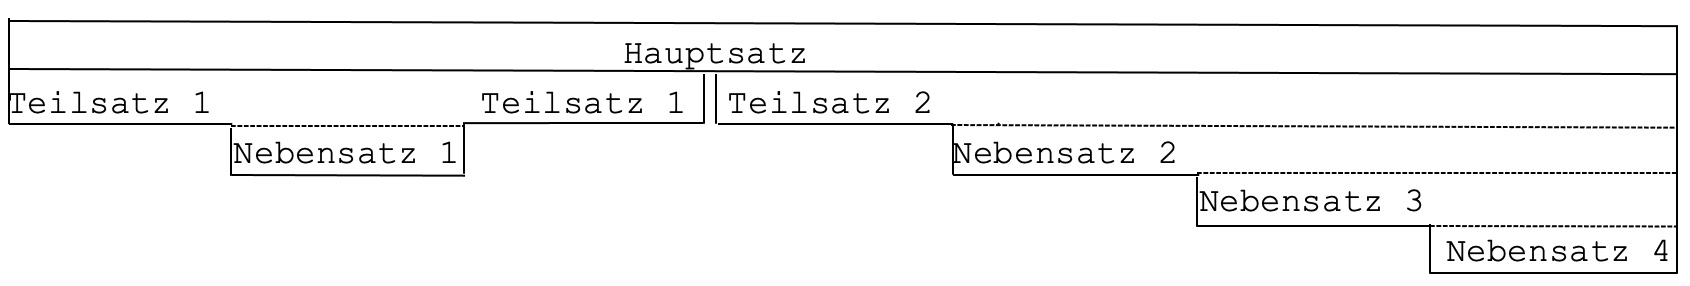
\includegraphics[width=12.5cm]{figures/Satzbild_Seghers}
    %% Abbildung 


\noindent\resizebox{\textwidth}{!}{
	
\begin{tabular}{ p{1.5cm} p{1.5cm} p{1.5cm} p{1.5cm} p{1.5cm} p{1.5cm} p{1.5cm} }
	
	\hline
	
	\multicolumn{7}{ | c | }{\hspace{2.5cm}\makecell[l]{\small\textcolor{gray}{Hauptsatz}}}  \\ \sbdashline{1-7} 
	
	\multicolumn{1}{ | l }{\makecell[l]{\small\textcolor{gray}{Teilsatz 1}}} &  
	\multicolumn{1}{l}{} & 	
	\multicolumn{1}{ l }{\makecell[l]{\small\textcolor{gray}{}}} &
	\multicolumn{4}{|| l | }{\makecell[l]{\small\textcolor{gray}{Teilsatz 2}}} \\ 
	\cline{1-1} \sbdashline{2-2} \cline{3-3}  \cline{4-4} \sbdashline{5-7}
	
	& \multicolumn{1}{ | l | }{\makecell[l]{\small\textcolor{gray}{Nebensatz 1}}} & & & 
	\multicolumn{3}{ | l | }{\makecell[l]{\small\textcolor{gray}{Nebensatz 2}}} \\ \cline{2-2} \cline{5-5} \sbdashline{6-7}
	
	& & & & & 
	\multicolumn{2}{ | l | }{\makecell[l]{\small\textcolor{gray}{Nebensatz 3}}} \\  \cline{6-6} \sbdashline{7-7}
	
	& & & & & &
	\multicolumn{1}{ | l | }{\makecell[l]{\small\textcolor{gray}{Nebensatz 4}}} \\  \cline{7-7}
	
	
\end{tabular}

}


	

    \caption{Satzbild zu (\ref{ea:Seghers_Satz})}
    \label{Abb:Satzbild_Seghrs}
\end{figure}


Der erste Nebensatz \textit{als ich krank und besinnungslos lag} ist ein Satzglied des ersten Teilsatzes. Es sättigt keine Valenzstelle des Hauptprädikats \textit{hatte gehofft}, sondern bestimmt den Zeitaspekt des Hauptsatzgeschehens und ist somit ein temporales Adverbial. Wir können den Nebensatz voranstellen (\ref{ea:Seghers_Satz_1_Nebensatz_Top}) und durch \textit{wann} ersetzen (\ref{ex:Seghers_Satz_1_Nebensatz_Frage}).

\ea \label{ea:Seghers_Satz_1_Nebensatz}
\ea \label{ea:Seghers_Satz_1_Nebensatz_Top} \textit{Als ich krank und besinnungslos lag}, hatte ich sogar manchmal auf jenen alten, frühen Namen gehofft.
\ex \label{ex:Seghers_Satz_1_Nebensatz_Frage} \textit{Wann} hatte ich sogar manchmal auf jenen alten, frühen Namen gehofft?
\z 
\z 

Die beiden Valenzstellen von \textit{hatte gehofft} werden durch \textit{ich} als Subjekt und \textit{auf jenen alten, frühen Namen} als Präpositionalobjekt gesättigt. Auch \textit{manchmal} ist ein Satzglied. Es drückt als temporales Adverbial aus, wie oft das Geschehen stattfand. 

Die Bestimmung von \textit{sogar} ist etwas komplizierter. Es drückt Erstaunen über etwas aus, hebt etwas als unerwartet hervor. Typischerweise fokussiert es als Attribut eine NP (\textit{sogar ich}/\textit{ich sogar}) oder eine PP (\textit{sogar auf jenen alten, frühen Namen}). Der Bezug wird durch die Stellung und die Betonung der fokussierten Größe deutlich. In dem Satz (\ref{ea:Seghers_Satz}) spricht die Stellung von \textit{sogar} jedoch für einen direkten Bezug auf das Hoffen-Szenario im Sinne von (\ref{ea:Seghers_Satz_sogar}).

\ea \label{ea:Seghers_Satz_sogar} Es war sogar so, dass ich manchmal, als ich krank und besinnungslos lag, auf jenen alten, frühen Namen hoffte.
\z 

Wir bestimmen \textit{sogar} als Kommentaradverbial (vgl. Abschnitt~\ref{subsection:Adverbial}). Die Schreiberin bewertet mit ihm das Hoffen-Szenario als etwas Erstaunliches, Besonderes. Für diese Bestimmung spricht die, wenn auch sehr markierte, alleinige Voranstellbarkeit von \textit{sogar} (\ref{ea:Seghers_Satz_sogar_Top}). 

\ea \label{ea:Seghers_Satz_sogar_Top} Sogar hoffte ich manchmal, als ich krank und besinnungslos lag, auf jenen alten, frühen Namen.
\z 

Hält man diese Stellung für unakzeptabel, dann wäre \textit{sogar} als Fokuspartikel ohne Satzgliedstatus zu bestimmen.

Innerhalb des Temporaladverbials \textit{als ich krank und besinnungslos lag} bildet \textit{lag} das Prädikat. Typischerweise verlangen sogenannte Positionsverben aufgrund ihrer Bedeutung nach einer Ergänzung in Form einer Lokalrelation wie \textit{im Bett liegen}. Analog kann jene Valenzstelle modal wie eben \textit{krank liegen} gesättigt werden. Bei anderen Verben würde es sich um ein Modaladverbial handeln. Da es sich hier um eine valenzielle Sättigung handelt, bestimmen wir \textit{krank und besinnungslos} als Modalergänzung.\footnote{Im Abschnitt~\ref{subsection:Adverbial} wurde jener zusätzliche Satzgliedtyp durch unseren valenziellen Ansatz begründet.}

Der nächste Teilsatz \textit{doch der Name blieb verloren} wird durch die Konjunktion \textit{doch} eingeleitet. Da sie weder Satzglied noch Attribut ist, wird sie in der Satzgliedanalyse nicht bestimmt. Das Prädikat \textit{blieb} verlangt als Kopulaverb nach einem Subjekt und nach einem Subjektsprädikativ (vgl. Abschnitt~\ref{subsection:SP und OP}). Diese Satzgliedfunktion übernimmt \textit{verloren}. Das Subjekt ist komplex, da die NP \textit{der Name} den appositiven Relativsatz mit weiteren eingebetteten Nebensätzen \textit{von dem ich in Selbsttäuschung glaubte, er könnte mich wieder gesund machen, jung, lustig, bereit zu dem alten Leben mit den alten Gefährten, das unwiederbringlich verloren war} als Attribut einbettet. Dass es sich bei dem ins Nachfeld ausgelagerten Komplex um einen Teil des Subjekts handelt, wird deutlich, wenn wir ihn zusammen mit seiner Bezugs-NP ins Vorfeld stellen (\ref{ea:Seghers_Satz_von_dem_Top}).

\ea \label{ea:Seghers_Satz_von_dem_Top} \textit{Doch der Name, von dem ich in Selbsttäuschung glaubte, er könnte mich wieder gesund machen, jung, lustig, bereit zu dem alten Leben mit den alten Gefährten, das unwiederbringlich verloren war,} blieb verloren.
\z 

Das Prädikat des Relativsatzes ist \textit{glaubte}. In der Bedeutung \gq{jemand meint in Bezug auf jemanden/etwas etwas} verlangt es nach drei Ergänzungen. Die erste Ergänzung \textit{ich} fungiert als Subjekt. Die PP \textit{von dem} ist Präpositionalobjekt. Der Inhalt des Glaubens wird durch den verkappten Nebensatz \textit{er könnte mich wieder gesund machen, jung, lustig, bereit zu dem alten Leben, mit den alten Gefährten, das unwiederbringlich verloren war} als Satzobjekt gesättigt. Dass dieser Komplex zusammen \textit{ein} Satzglied zum Prädikat \textit{glaubte} bildet, zeigt sich bei Pronominalisierung (\ref{ea:Seghers_Satz_glaubte_das}) sowie bei Voranstellung im umformulierten Hauptsatz (\ref{ex:Seghers_Satz_das_glaubte_HS}).

\ea \label{ea:Seghers_Satz_glaubte}
\ea \label{ea:Seghers_Satz_glaubte_das} Doch der Name, von dem ich \textit{das} in Selbsttäuschung glaubte, blieb verloren.
\ex \label{ex:Seghers_Satz_das_glaubte_HS} \textit{Er könnte mich wieder gesund machen, jung, lustig, bereit zu dem alten Leben, mit den alten Gefährten, das unwiederbringlich verloren war}, glaubte ich in Selbsttäuschung von dem Namen.
\z 
\z 

Die PP \textit{in Selbsttäuschung} ist ein Satzglied, das keine Valenzstelle sättigt. Es drückt eine Art und Weise des Glauben-Szenarios aus und ist somit ein modales Adverbial. Sinnvoll interpretieren wir es eher kausal als \gq{durch Selbsttäuschung}.

Das Satzobjekt zu \textit{glaubte} besteht intern wieder aus Satzgliedern. Sein Prädikat ist komplex und besteht aus dem Prädikat \textit{könnte machen} und den Objektsprädikativen \textit{wieder gesund}, \textit{jung}, \textit{lustig} und \textit{bereit}.\footnote{Auf \textit{wieder} gehen wir bei der Attributanalyse genauer ein.} Durch Koordination wird \textit{machen} als identischer Bestandteil jeweils ausgelassen. Da wir im Abschnitt~\ref{subsection:SP und OP} Objektsprädikative mikrovalenziell als Prädikatsteile bestimmt haben, stehen die Objektsprädikative \textit{jung}, \textit{lustig} und \textit{bereit} elliptisch für \textit{jung machen}, \textit{lustig machen} und \textit{bereit machen}. Wir analysieren sie daher getrennt als vier Objektsprädikative stellvertretend für koordinierte Prädikate. Als Subjekt fungiert \textit{er} und als Akkusativobjekt \textit{mich}. Durch das vierte Objektsprädikativ \textit{bereit} kommt es zu einer Valenzerhöhung. Die neue Valenzstelle wird durch die PP \textit{zu dem alten Leben mit den alten Gefährten, das unwiederbringlich verloren war} als Präpositionalobjekt gesättigt.   

Der appositive Relativsatz \textit{das unwiederbringlich verloren war} gehört zu \textit{dem alten Leben mit den alten Gefährten} und ist deshalb Teil des Präpositionalobjekts \textit{zu dem alten Leben mit den alten Gefährten, das unwiederbringlich verloren war}. Wird das Präpositionalobjekt wie in (\ref{ea:Seghers_Satz_dazu_bereit}) durch \textit{dazu} pronominalisiert, verschwindet auch der Relativsatz. Bei Voranstellung des Präpositionalobjekts im umformulierten Hauptsatz steht auch der Relativsatz als Satzgliedteil im Vorfeld (\ref{ex:Seghers_Satz_zu_dem_alten_Leben_HS}).

\ea \label{ea:Seghers_Satz_bereit_zu}
\ea \label{ea:Seghers_Satz_dazu_bereit} Doch der Name blieb verloren, von dem ich in Selbsttäuschung glaubte, er könnte mich wieder gesund machen, jung, lustig, \textit{dazu} bereit.
\ex \label{ex:Seghers_Satz_zu_dem_alten_Leben_HS} \textit{Zu dem alten Leben mit den alten Gefährten, das unwiederbringlich verloren war,} könnte er mich bereit machen.
\z 
\z 

Das Zentrum des Relativsatzes bildet die Kopulaform \textit{war} als Prädikat. Das den Relativsatz einleitende Demonstrativpronomen \textit{das} fungiert als Subjekt. Da es sich um ein Kopulaverb handelt, verlangt es nach einem Subjektsprädikativ. Diese Funktion erfüllt \textit{unwiederbringlich verloren}. Bei der Attributanalyse kommen wir auf die Beziehung zwischen \textit{unwiederbringlich} und \textit{verloren} zurück.   

Die Analyse wird in der Tabelle~\ref{tab:Seghers_Satz} gezeigt.

\begin{table}
%\tiny   
  \centering
  \resizebox{\textwidth}{!}{
  \begin{tabular}{l|l|l|l|l}
   % \lsptoprule
       &  Hauptsatz  &  1. NeSa-Ebene  & 2. NeSa-Ebene & 3. NeSa-Ebene \\
    \hline
    \textit{Ich} & Subjekt 1 & & & \\ \cline{2-2}
    \textit{hatte} & Prädikat 1 & & & \\ \cline{2-2} 
    \textit{sogar,} & Kommentaradverbial 1 & & & \\ \cline{2-2}
    \textit{als} & \multirow{6}{*}{Adverbial 1} & -- & & \\ \cline{3-3}
    \textit{ich} & & Subjekt & & \\ \cline{3-3}
    \textit{krank} & & \multirow{3}{*}{Modalergänzung} & & \\
    \textit{und} & & & & \\
    \textit{besinnungslos} & & & & \\ \cline{3-3}
    \textit{lag,} & & Prädikat & & \\ \cline{2-3}
    \textit{manchmal} & Adverbial 1 & & & \\ \cline{2-2}
    \textit{auf} & \multirow{5}{*}{Präpositionalobjekt 1} & & & \\ 
    \textit{jenen} & & & & \\ 
    \textit{alten} & & & & \\ 
    \textit{frühen} & & & & \\ 
    \textit{Namen} & & & & \\ \cline{2-2}
    \textit{gehofft,} & Prädikat 1 & & & \\ \cline{2-2}
    \textit{doch} & -- & & & \\ \cline{2-2}
    \textit{der} & \multirow{2}{*}{Subjekt 2} & & & \\ 
    \textit{Name} & & & & \\ \cline{2-2}
    \textit{blieb} & Prädikat 2 & & & \\ \cline{2-2} 
    \textit{verloren,} & Subjektsprädikativ 2 & & & \\ \cline{2-3}
    \textit{von} & \multirow{27}{*}{Subjekt 2} & \multirow{2}{*}{Präpositionalobjekt} & & \\ 
    \textit{dem} & & & & \\ \cline{3-3}
    \textit{ich} & & Subjekt & & \\ \cline{3-3}
    \textit{in} & & \multirow{2}{*}{Adverbial} & & \\ 
    \textit{Selbsttäuschung} & & & & \\ \cline{3-3}
    \textit{glaubte,} & & Prädikat & & \\ \cline{3-4}
    \textit{er} & & \multirow{21}{*}{Satzobjekt} & Subjekt & \\ \cline{4-4}
    \textit{könnte} & & & Prädikat & \\ \cline{4-4}
    \textit{mich} & & & Akkusativobjekt & \\ \cline{4-4}
    \textit{wieder} & & & \multirow{2}{*}{Objektsprädikativ 1} & \\ 
    \textit{gesund} & & & & \\ \cline{4-4}
    \textit{machen,} & & & Prädikat 1--4 \\ \cline{4-4}
    \textit{jung,} & & & Objektsprädikativ 2 & \\ \cline{4-4}
    \textit{lustig,} & & & Objektsprädikativ 3\\ \cline{4-4}
    \textit{bereit} & & & Objektsprädikativ 4 \\ \cline{4-4}
    \textit{zu} & & & \multirow{12}{*}{Präpositionalobjekt zu 4} & \\
    \textit{dem} & & & & \\
    \textit{alten} & & & & \\ 
    \textit{Leben} & & & & \\ 
    \textit{mit} & & & & \\ 
    \textit{den} & & & & \\
    \textit{alten} & & & & \\
    \textit{Gefährten,} & & & & \\ \cline{5-5}
    \textit{das} & & & & Subjekt \\ \cline{5-5}
    \textit{unwiederbringlich} & & & & \multirow{2}{*}{Subjektsprädikativ} \\
    \textit{verloren} & & & & \\ \cline{5-5}
    \textit{war.} & & & & Prädikat \\ 
    \hline 
   % \lspbottomrule
  \end{tabular}
  }
  \caption{Seghers-Satz}
  \label{tab:Seghers_Satz}
\end{table}

Kommen wir nun zu den Attributen innerhalb der ermittelten Satzglieder. Innerhalb des Präpositionalobjekts \textit{auf jenen alten, frühen Namen} beziehen sich \textit{alten} und \textit{frühen} als Adjektivattribute gleichrangig auf das Nomen \textit{Namen} als Bezugswort. Orthografisch wird die Gleichrangigkeit durch das Komma gekennzeichnet. 

Innerhalb der komplexen Subjekt-NP \textit{der Name, von dem ich in Selbsttäuschung glaubte, er könnte mich wieder gesund machen, jung, lustig, bereit zu dem alten Leben mit den alten Gefährten, das unwiederbringlich verloren war} bezieht sich der Relativsatz, zusammen mit den in ihn eingebetteten Nebensätzen, als Attribut appositiv auf \textit{der Name}. Allerdings folgt dieses komplexe Attribut nicht direkt seinem Bezugsausdruck, sondern steht, ausgeklammert, im Nachfeld.

Innerhalb des komplexen Objektsprädikativs \textit{wieder gesund} bezieht sich das Adverb \textit{wieder} attributiv auf sein Bezugsadjektiv \textit{gesund}. Diese Bestimmung ist durch die Lesart von \textit{wieder} motiviert. Hier geht es nicht um die Wiederholung des Geschehens \textit{gesund machen} im Sinne von \gq{noch einmal gesund machen}, sondern um die Wiederherstellung des Zustands \textit{gesund}.

Das Präpositionalobjekt \textit{zu dem alten Leben mit den alten Gefährten, das unwiederbringlich verloren war} ist durch verschiedene Attributbeziehungen komplex. Das Adjektiv \textit{alten} bezieht sich attributiv auf das Substantiv \textit{Leben} als Bezugswort. Die PP \textit{mit den alten Gefährten} bezieht sich ebenfalls als Attribut auf \textit{Leben}. Formal lässt sich keine Hierarchie zwischen den beiden Attributen ausmachen, also ob \textit{alten} Attribut zu \textit{Leben mit den alten Gefährten} ist oder ob \textit{mit den alten Gefährten} Attribut zu \textit{alten Leben} ist. Semantisch können wir die Eigenschaft \gq{alt} auf \textit{Leben mit den alten Gefährten} beziehen. Wir können aber auch \textit{mit den alten Gefährten} als eine Art näherer Bestimmung des \gq{alten Lebens} verstehen.

Innerhalb der attributiven PP \textit{mit den alten Gefährten} fungiert das Adjektiv \textit{alten} als Attribut zu \textit{Gefährten}. 

Der Relativsatz \textit{das unwiederbringlich verloren war} bezieht sich attributiv auf \textit{das alte Leben mit den alten Gefährten}. Hierfür spricht der appositive Charakter des Relativsatzes. Denn er dient nicht dazu, den Referenzbereich von \textit{Leben} einzugrenzen, sondern ist eine zusätzliche Information zu \textit{dem alten Leben mit den alten Gefährten}. Hierfür spricht die Möglichkeit, \textit{übrigens} einzufügen: \textit{das alte Leben mit den alten Gefährten, das übrigens unwiederbringlich verloren war}. 

Innerhalb des Subjektsprädikativs \textit{unwiederbringlich verloren}, bezieht sich das Adjektiv \textit{unwiederbringlich} attributiv auf \textit{verloren}. 
